\documentclass[german,version-2020-11]{uzl-thesis}

% % % % % % % %
% Packages
% % % % % % % %

%?
\usepackage{tabularx}
\usepackage{longtable}
\usepackage{parskip}
\setlength{\parindent}{0pt}
\setlength{\mathindent}{0pt}
%/?

\usepackage{pgfplots}

\usepackage{multirow}
\usepackage{fancyvrb}
\usepackage{tikz,lipsum,lmodern}
\usepackage[most]{tcolorbox}
\usepackage{float}
\usepackage[german]{struktex}

%\usepackage{arydshln}

\pgfplotsset{compat=1.18}

% % % % % % % %
% Environments
% % % % % % % %

\newenvironment{customIndentRight}{

\setlength{\leftskip}{1.5cm}
\setlength{\rightskip}{1.5cm}}{

\setlength{\leftskip}{0cm}
\setlength{\rightskip}{0cm}}

\newenvironment{customIndentRight2}{

\setlength{\leftskip}{1.0cm}
\setlength{\rightskip}{1.0cm}}{

\setlength{\leftskip}{0cm}
\setlength{\rightskip}{0cm}}

% % % % % % % %
% Commands
% % % % % % % %

\newcommand{\newpara}[1]{
\vspace{0.7em}{\bfseries #1}
}

\newcommand{\heightNS}{8}

\newcommand{\struktogrammA}[3]{
\begin{centernss}
\small
\begin{struktogramm}(170,#1)[#2]
#3
\end{struktogramm}
\end{centernss}
}

\newcommand{\struktogrammAO}[2]{
\begin{centernss}
\small
\begin{struktogramm}(170,#1)
#2
\end{struktogramm}
\end{centernss}
}

\newcommand{\struktkommentar}[1]{
\begin{customIndentRight2}
\small
#1
\end{customIndentRight2}
%\begin{centernss}
%\small
%#1
%\end{centernss}
}

\newcommand{\abstandLinksDataInt}{
16pt
}

\newcommand{\umsteigerTabelleInnenWeite}{
.57\textwidth
}

\newcommand{\umsteigerTabelleCodeBreak}{
\\[-2pt]
}
\newcommand{\umsteigerTabelleCodeBreakEnd}{
\\[-10pt]
}
\newcommand{\umsteigerTabelleSonstiges}[1]{
\begin{minipage}[t]{\umsteigerTabelleInnenWeite}%\vspace{-7pt}
\begin{itemize}[leftmargin=*] #1 \end{itemize}
\end{minipage}
}

\begin{comment}
\newcommand{\umsteigerTabelleAnmerkung}[1]{
\multicolumn{3}{ |l| }{\emph{Anmerkung:}
\begin{minipage}[t]{.75\textwidth}
#1 %\vspace{3pt}
\end{minipage}
} \\
}
\end{comment}

\newcommand{\umsteigerTabelleZeile}[3]{
#1 & #2 & #3 \\
\hline
}

\newcommand{\umsteigerTabelleKopf}{
\textbf{Version} & \multicolumn{2}{ c| }{\textbf{Abweichungen zwischen den Versionen}} \\
}

\newcommand{\umsteigerTabelleZeileU}[2]{
#1 & URL & \texttt{#2}  \\ \cline{2-3}
}

\newcommand{\umsteigerTabelleZeileUCU}[4]{
\multirow{2}{*}{#1} & URL & \texttt{#2}  \\ \cline{2-3}
& Kodes & \begin{minipage}[t]{\umsteigerTabelleInnenWeite} \texttt{#3} \end{minipage} \\ \cline{2-3}
& Umsteiger & \begin{minipage}[t]{\umsteigerTabelleInnenWeite} \texttt{#4} \end{minipage} \\ \cline{2-3}
}

\newcommand{\umsteigerTabelleZeileUU}[3]{
\multirow{2}{*}{#1} & URL & \texttt{#2}  \\ \cline{2-3}
& Umsteiger & \begin{minipage}[t]{\umsteigerTabelleInnenWeite} \texttt{#3} \end{minipage} \\ \cline{2-3}
}

\newcommand{\umsteigerTabelleZeileUCUS}[5]{
\multirow{2}{*}{#1} & URL & \texttt{#2}  \\ \cline{2-3}
& Kodes & \begin{minipage}[t]{\umsteigerTabelleInnenWeite} \texttt{#3} \end{minipage} \\ \cline{2-3}
& Umsteiger & \begin{minipage}[t]{\umsteigerTabelleInnenWeite} \texttt{#4} \end{minipage} \\ \cline{2-3}
& Sonstiges & \umsteigerTabelleSonstiges{#5}  \\ \cline{2-3}
}

\newcommand{\umsteigerTabelleZeileUS}[3]{
\multirow{2}{*}{#1} & URL & \texttt{#2}  \\ \cline{2-3}
& Sonstiges & \umsteigerTabelleSonstiges{#3}  \\ \cline{2-3}
}

\newcommand{\umsteigerTabelleZeileUV}[3]{
\multirow{2}{*}{#1} & URL & \texttt{#2}  \\ \cline{2-3}
& Verzeichnis & \texttt{#3}  \\ \cline{2-3}
}

\newcommand{\umsteigerTabelleZeileLetzte}[3]{
\multirow{2}{*}{#1} & Kodes & \begin{minipage}[t]{\umsteigerTabelleInnenWeite} \texttt{#2} \end{minipage} \\ \cline{2-3}
& Sonstiges & \umsteigerTabelleSonstiges{#3}  \\ \cline{2-3}
}

\newcommand{\jsonBox}[2]{
\begin{tcolorbox}[center,width=#1\textwidth,
    colback=white,colframe=black,boxrule=.5pt]
\texttt{#2}
\end{tcolorbox}
}

\newcommand{\codeBox}[2]{
\begin{tcolorbox}[center,width=#1\textwidth,
    colback=white,colframe=black,boxrule=.5pt]
\texttt{#2}
\end{tcolorbox}
}

\newcommand{\codeBoxL}[1]{
\begin{tcolorbox}[width=.34\textwidth,
    colback=white,colframe=black,boxrule=.5pt]
\texttt{#1}
\end{tcolorbox}
\vspace{-4pt}
}

\newcommand{\codeBoxLD}[2]{
\begin{tcolorbox}[width=.34\textwidth,
    colback=white,colframe=black,boxrule=.5pt]
\texttt{#1}
\tcblower
\texttt{#2}
\end{tcolorbox}
\vspace{-4pt}
}

\newcommand{\codeBoxDouble}[3]{
\begin{tcolorbox}[center,width=#1\textwidth,
    colback=white,colframe=black,boxrule=.5pt]
\texttt{#2}
\tcblower
\texttt{#3}
\end{tcolorbox}
}



%%%
%
% Main setup:
%
%%%
%
% You must use the \UzLThesisSetup command to specify numerous things
% about your thesis. This includes the entries on the title page, the 
% abstracts, and the bibliography style. You do so by specifying
% so-called "values" for so-called "keys". For instance, 
% for the key "Autor" you must provide your name as the value. You do
% so by writing 'Autor = {Max Mustermann}', that is, the value is put
% into curly braces. You can use the \UzLThesisSetup command
% repeatedly and the order in which you provide the keys is not
% important. 
%
% Everything shown on the title page must be in German -- even
% if the thesis is written in English! Just insert German text for
% German keys and English text for English keys (like 'Abstract' needs
% English text, while 'Zusammenfassung' needs German text).

\UzLThesisSetup{
  Logo-Dateiname        = {uzl-thesis-logo-itcs.pdf},
  Verfasst              = {am}{Institut für Medizinische Informatik},
  Titel auf Deutsch     = {Abbilden und Nutzen von Versionsübergreifenden Medizinischen Klassifikationen mittels FHIR ConceptMaps},
  Titel auf Englisch    = {Visualization and Mapping of Medical Classifications across Multiple Versions with FHIR ConceptMaps},
  Autor                 = {Simon Müller},
  Betreuer              = {Prof. Dr. Josef Ingenerf},
  Mit Unterstützung von = {Tessa Ohlsen, M. Sc.},
  Masterarbeit,
  Studiengang           = {Medizinische Informatik},
  Datum                 = {1. November 2024},
  %
  % The English abstract. You must always provide abstracts in German
  % and in English. 
  %
  Abstract              = {
  },
  Zusammenfassung       = {
  },
  Alphabetische Bibliographie,
}

\UzLStyle{pagella basic design}

\addbibresource{../draft/intro.bib}
\addbibresource{../draft/data1.bib}
\addbibresource{../draft/data2.bib}
\addbibresource{../draft/tech.bib}
\addbibresource{../draft/fin.bib}

\begin{document}

%\input{thesis_sub.tex}

\chapter{Einleitung} \begin{comment}
\bibitem{medinf-init}
Medizininformatik-Initiative \newline
\url{https://www.medizininformatik-initiative.de/de/start}
% Der Druck andererseits ist groß, mit vorhandenen Versorgungsdaten (insb. in der Medizininformatik-Initiative (LINK), in der auch wir aktiv sind) für die Forschung zu arbeiten.

\bibitem{fdpg}
Deutsches Forschungsdatenportal für Gesundheit \newline
\url{https://forschen-fuer-gesundheit.de}
% Hierzu gibt es eine Forschungsdaten für Gesundheits-Plattform (LINK), wo im großen Stil Daten aus sogenannten Datenintegrationszentren (DIZ) aus etwa 30 Universitätskliniken in Deutschland föderiert abgefragt werden. 
\end{comment}

Das Bundesinstitut für Arzneimittel und Medizinprodukte, kurz: BfArM, veröffentlicht jedes Jahr aktualisierte Versionen medizinischer Klassifikationen, wie zum Beispiel der Kodiersysteme ICD-10-GM und OPS. Diese Änderungen in den Kodes erschweren die versionsübergreifende Analyse klinischer Daten, wie sie beispielsweise vom Deutsches Forschungsdatenportal für Gesundheit \cite{medinf-init} zur Verfügung gestellt werden. Ein technischer Ansatz dieses Code-Mapping-Problem zu lösen wäre die Verwendung von \emph{ConceptMaps} aus dem FIHR Standards für den Austausch elektronischer Gesundheitsdaten.

\section{Grundbegriffe}
\subsection{Klassifikationen ICD-10-GM und OPS}

Diese Arbeit bezieht sich auf die Systematischen Verzeichnisse von ICD-10-GM und OPS, das heißt der nach dem Kode strukturierten Veröffentlichungen dieser Kodiersysteme. 

\newpara{ICD-10-GM}

Zitiert aus \cite[Seite 97]{gaus2005dokumentation}:

\quoteBox{
Die International Statistical Classification of Diseases (ICD) geht auf das Jahr 1855 zurück
[...] und wird heute von der World Health Organisation (WHO) betreut. Die
10. Revision trat am 01.01.1993 in Kraft unter der Bezeichnung [...] ICD-10. Die deutschen
Ausgaben werden vom Deutschen Institut für Medizinische Dokumentation und Information (DIMDI)
als dem WHO Kooperationszentrum erarbeitet. Die am 01.01.2005 in Kraft
getretene Ausgabe heißt [...] ICD-10-GM 2005, wobei GM für German Modification steht.
}

Seit Mai 2020 ist das DIMDI in das BfArM eingegliedert. \cite{bfarmdimdi}

\newpage

Wiederum \cite[Seite 98ff]{gaus2005dokumentation}:

\quoteBox{
Die ICD-10-GM 2005 ist ein Ordnungssystem für \emph{Krankheiten (Diagnosen)}, das nach dem
\emph{Ordnungsprinzip Klassifikation} aufgebaut ist und insgesamt ca. 64 000 Klassen hat. Die
\emph{Notation} ist vier- oder fünfstellig. Sie besteht aus einem Buchstaben, einer zweistelligen
Zahl, einem Punkt (dient nur der Strukturierung, liefert keine Information und wird deshalb
bei der Stellenzahl nicht mitgezählt) und dann noch eine (vierstellige Notation) oder zwei
(fünfstellige Notation) einstellige Zahlen. [...] \\

Die ICD-10-GM 2005 ist hierarchisch geordnet. Bei der Notation bezeichnen die 3 Stellen
vor dem Punkt ein hierarchisches Niveau, das Raum für 2 500 gleichgeordnete Klassen bietet
und nur durch Überschriften weiter gegliedert ist. Die Stellen nach dem Punkt geben weitere
Niveaus an, d.h. die vierstellige Notation beschreibt 2, die fünfstellige Notation 3 hierarchische Niveaus. [...] \\

Ein allgemeines Problem der systematischen Anordnung von Diagnosen ist, ob eine Diagnose unter dem Ort ihrer Manifestation oder unter dem ihr zugrunde liegenden Krankheitsprozess eingeordnet werden soll. \emph{Beispiel:} Soll die Lungenentzündung unter der Lokalisation
Lunge oder unter dem Krankheitsprozess Entzündung eingeordnet werden? Werden alle
Krankheiten eines bestimmten Organs nebeneinander gestellt, so folgt die Systematik dem
topologisch-organspezifischen Aspekt (\emph{Topologie} = Lehre von der Lage und Anordnung der
Dinge im Raum). In einer Systematik können jedoch auch alle Krankheiten mit dem gleichen
Krankheitsprozess, z.B. alle Entzündungen, alle Autoimmunkrankheiten oder alle bösartigen
Neubildungen, nebeneinander gestellt werden. Diese Einteilung nennt man ätiologisch,
pathologisch oder nosologisch (\emph{Ätiologie} = die Krankheit auslösende Ursache, \emph{Pathologie
und Nosologie} = Lehre von den Krankheiten). Dieses Problem ist mit dem Ordnungsprinzip
Klassifikation nicht lösbar. Die [ICD-10-GM] benutzt im Wesentlichen den ätiologischen Aspekt.
}

Definition des Begriffs Klassifikation aus \cite[Seite 86f]{gaus2005dokumentation}:

\quoteBox{Von allen Ordnungsprinzipien ist die Klassifikation das einfachste. Es beruht auf dem
Grundsatz: "`Jedes Ding (jeder Sachverhalt) an seinen Platz"'. Das zu dokumentierende Sachgebiet wird in einzelne \emph{getrennte Sachverhalte} eingeteilt, die man als \emph{Klassen} bezeichnet. [...]
Die Klassen sind \emph{disjunkt}, d.h. sie schließen sich gegenseitig aus und überlappen sich nicht. Jede Klasse wird
durch einen Deskriptor repräsentiert. Die Klassen einer Klassifikation sind gleichzeitig
\emph{Äquivalenzklassen} von Begriffen. Im strengen Fall ist die Zuordnung einer Dokumentationseinheit zu einer Klasse eindeutig, d.h. eine Dokumentationseinheit wird genau einer
Klasse zugeteilt. Eine Klassifikation ist einfach und praktisch. Sie ist sozusagen das \emph{"`natürliche Ordnungsprinzip"'}. [...] \\

Ein \emph{Klassifikationssystem} -- ein Ordnungssystem, das nach dem Ordnungsprinzip Klassifikation aufgebaut ist -- muss vollständig sein. Vollständig sein bedeutet, dass die Klassen alle
Sachverhalte des dokumentarisch zu bearbeitenden Sachgebiets umfassen. [...] Durch Schaffung einer Klasse \emph{"`sonstiges"'} oder besser
durch die Schaffung mehrerer Klassen mit dem Zusatz „sonstiges“ wird
die geforderte Vollständigkeit des Klassifikationssystems [...]
formal erreicht. [...] Um auf die einzelnen Klassen bequem und sicher zugreifen zu können, werden sie \emph{hierarchisch} oder anderweitig \emph{systematisch} angeordnet.

%Um auf die einzelnen Klassen bequem und sicher zugreifen zu können, werden sie hierarchisch oder anderweitig systematisch angeordnet. [...]%Eine hierarchische oder anderweitig systematische Anordnung trägt, wie in den beiden folgenden Themen ausführlich behandelt wird, erheblich zur terminologischen Kontrolle bei. In der Klassifikation verbindet sich also das einfachste Ordnungsprinzip und die einfachste Form der terminologischen Kontrolle. Deshalb sind Klassifikationen weit verbreitet.
}

\newpage

Vom BfArM werden Notation und Begriff bezeichnet als Kode und Titel.

\newpara{OPS}

Ebenfalls zitiert aus \cite[Seite 101ff]{gaus2005dokumentation}:

\quoteBox{
In der Medizin werden nicht nur Krankheiten, sondern auch ärztliche Tätigkeiten dokumentarisch erfasst und – ebenso wie die Diagnosen für die Abrechnung und für wissenschaftliche
Zwecke verwendet. Die von der WHO erstmals 1978 herausgegebene International Classification of Procedures in Medicine (ICPM) wurde (ebenso wie die ICD-10) vom DIMDI ins
Deutsche übertragen und an deutsche Verhältnisse angepasst. Die am 01.01.2005 in Kraft
getretene Ausgabe heißt "`Operationen- und Prozedurenschlüssel -- Internationale Klassifikation der Prozeduren in der Medizin (OPS 2005)"'. Der OPS 2005 ist – wie die Bezeichnung \emph{"`Schlüssel"'} ausdrückt – eine Klassifikation mit numerischer Notation. Allerdings haben in einigen Bereichen die 10 gleichgeordneten Klassen nicht ausgereicht, deshalb treten
an der 5. und 6. Stelle der Notation gelegentlich Buchstaben auf. Von den insgesamt
14 000 Klassen betreffen etwa 70\% Operationen, ca. 15\% nichtoperative therapeutische
Maßnahmen, 8\% diagnostische Maßnahmen, 4\% bildgebende Diagnostik und 2\% ergänzende Maßnahmen. \\

Die \emph{Notation} des OPS 2005 ist vier- bis sechsstellig. Die erste Stelle enthält eine 1, 3, 5, 8
oder 9 und bezeichnet einen der eben genannten Bereiche (z.B. 1 = diagnostische Maßnahmen). Es folgt ein Bindestrich und eine dreistellige Zahl. Je nach Detaillierungsgrad ist damit
die Notation beendet oder es folgen noch ein Punkt und weitere 1 bis 2 Stellen. [...] In der fünften und sechsten Stelle der Notation (d.h. nach dem Punkt) können Ziffern durch
die Buchstaben x oder y ersetzt werden, es bedeutet x = sonstige und y = nicht näher bezeichnet.
}

\subsection{FHIR ConceptMap}

FHIR steht für "`Fast Healthcare Interoperability Resources"'. 

\newpara{HL7 FHIR}

Zitiert aus \cite[Seite 309]{fhir-heckmann}: 

\quoteBox{
"`Health Level 7"' wurde 1987 gegründet, um Standards für klinische Informationssysteme
zu erarbeiten. [...] % Der Name der Organisation nimmt Bezug auf die siebte Schicht (Application Layer) des ISO/OSI-Modells, und bringt damit zum Ausdruck, dass hier die Festlegung von anwendungsbezogenen Inhalten und Prozessen im Vordergrund steht, nicht die Spezifikation von z. B. Ubertragungsprotokollen (HLT International, 2021).
HL7 ist vom nationalen amerikanischen Normeninstitut (ANSI) seit 1994 akkreditiert.
HL7-verbundene Organisationen existieren inzwischen in über 40 Ländern. Die erste
nationale Partnergesellschaft wurde 1993 in Deutschland gegründet. Die Aufgabe dieser
sogenannten "`Affiliates"' ist es, die Verbreitung und Implementierung der internationalen
HL7-Standards in dem jeweiligen Land zu fördern und gegebenenfalls erforderliche Anpassungen und Erweiterungen für deren Nutzung zu entwickeln. FHIR ist die dritte Generation von Interoperabilitätsstandards aus der Feder von HL7. \\

Die Entwicklung begann im Jahre 2011 als Reaktion auf die Forderungen aus der Industrie nach einer standardisierten Lösung für die Entwicklung webbasierter Applikationen für das Gesundheitswesen. %Der erste Entwurf der FHIR-Spezifikation stammt aus der Feder von Grahame Grieve (AUS), Ewout Kramer (NL) und Lloyd McKenzie (CAD). Erste stabile Versionen von FHIR wurden 2014 und 2015 mit dem Zusatz ,,DSTU* (Draft Standard for Trial Use) publiziert und bereits von der Industrie zur Implementierung genutzt. Insbesondere die Version DSTU 2 wurde in den USA schnell aufgegriffen, obgleich der «»DSTU*-Zusatz. den nicht-normativen Status dieser Publikationen hervorhebt. 2017 wurde die dritte Version unter der Bezeichnung ,STU3" publiziert.
[...] Die vierte, 2018 veröffentlichte Version "`R4"' enthält erstmals normative Inhalte. % Die Entwicklung des Standards ist damit jedoch noch nicht abgeschlossen. Mit Hilfe eines ausgekliigelten Reifegradmodelles wird der Entwicklungsstand einzelner Teile der Spezifikation regelmiibig bewertet. Normativen Status erhiilt ein Artefakt dann, wenn es geméi8 der Abstimmungsregein bei HL7 ballotiert, umfassend getestet und von mindestens fiinf unabhiingigen Hersteller in mehr als einem Land unter produktiven Bedingungen implementiert wurde. Damit wird sicher- gestellt, dass nichts normativ (und damit als weitgehend unvertinderlich) deklariert wird, was nicht ausfiihrlich auf seine Nutzbarkeit unter Echtbedingungen hin getestet wurde.
}

\newpage

Ebenfalls aus \cite[Seite 310]{fhir-heckmann}:

\quoteBox{
Im Gegensatz zu älteren HL7-Standards [...] bedient sich FHIR erstmals moderner webbasierter Technologien, die auch jenseits des Gesundheitswesens weit verbreitet und bei Entwicklern bekannt und beliebt sind. FHIR legt den Fokus auf die query-getriebene Art der
Kommunikation, die dazu dient, Anwendungen und Anwendern die benötigten Daten zum
benötigten Zeitpunkt in adäquatem Umfang und Format zur Verfügung zu stellen. Dazu
bedient sich FHIR dem Representational State Transfer (kurz: "`REST"'), einem Paradigma,
das die Struktur und das Verhalten des Word Wide Webs abstrahiert und basierend auf denselben Technologien und Grundlagen eine einheitliche Form der Kommunikation von verteilten Systemen und Webservices definiert. Die auszutauschenden Datenobjekte werden
als "`Ressourcen"' bezeichnet, auf denen jeweils sogenannte "`CRUD"'-Interaktionen (create, read, update, delete) über die HTTP-Methoden GET, PUT, POST und DELETE ausgeführt werden können.
%FHIR definiert auf dieser Grundlage etwa 150 verschiedene, im Gesundheitswesen reevante, Objekttypen (im REST-Kontext als ,.Ressourcentypen" bezeichnet) und deren Bezichungen untereinander (im REST-Kontext als ,.Links* bezeichnet) (Tab. 1),
%‘Zur Serialisierung der Ressourcen fir die Speicherung und Ubertragung erlaubt FHIR sowohl das JSON- als auch das XML-Format. Server-Applikationen sind angehalten,
}

Die Autorin hebt außerdem folgende Eigenschaften hervor:

\begin{itemize}
\item "`FHIR als Baukasten"': Standards und Leitfäden in FHIR sind selbst Ressourcen. Sie können erweitert und für verschiedene Zwecke eingesetzt werden. 
\item "`FHIR als Community-Standard"': Die FHIR-Spezifikation ist frei verfügbar und wird von einer Community entwickelt, statt von einem geschlossenen Gremium. 
\end{itemize}

Die am meisten verbreitetsten Implementationen von FHIR sind die als freie Software lizenzierte API-Server \emph{HAPI}, sowie der proprietäre Terminologie-Server \emph{Ontoserver}, welcher unter anderem im australischen Gesundheitssystem eingesetzt wird. Für mehr dazu siehe \cite{braunstein2022health}. 

\begin{comment}
«HL7\textsuperscript{\textregistered} FHIR\textsuperscript{\textregistered} (im Folgenden "`FHIR"' genannt) ist der modernste Interoperabilitäts-Stan-\newline dard aus der Produktfamilie von Health Level 7 International (kurz: "`HL7"'), einer internationalen Standardisierungsorganisation für das Gesundheitswesen, die in der Vergangenheit schon viele erfolgreiche und weit verbreitet genutzte Standards, wie zum Beispiel HL7 Version 2 oder HL7 CDA (Clinical Document Architecture) hervorgebracht hat. [...] HL7 wurde 1987 gegründet, um Standards für klinische Informationssysteme zu erarbeiten. [...] FHIR ist die dritte Generation von Interoperabilitätsstandards aus der Feder von HL7. Die Entwicklung begann im Jahre 2011 als Reaktion auf die Forderungen aus der Industrie nach einer standardisierten Lösung für die Entwicklung webbasierter Applikationen für das Gesundheitswesen.» \cite{fhir-heckmann}

"`Health Level 7 wurde 1987 gegründet, um Standards für klinische Informationssysteme zu erarbeiten. [...] FHIR ist die dritte Generation von Interoperabilitätsstandards aus der Feder von HLR7. Die Entwicklung begann im Jahre 2011 als Reaktion auf die Forderungen aus der Industrie nach einer standardistieren Lösung für die Entwicklung webbasierter Applikationen für das Gesundheitswesen."' \cite[Seite 309]{fhir-heckmann}



\begin{comment}
2 Einfiihrung in HL7* FHIR®

«Health Level 7* wurde 1987 gegriindet, um Standards fir klinische Informationssysteme
zu erarbeiten, Der Name der Organisation nimmt Bezug auf die siebte Schicht (Applica-
tion Layer) des ISO/OSI-Modells, und bringt damit zum Ausdruck, dass hier die Fest-
legung von anwendungsbezogenen Inhalten und Prozessen im Vordergrund steht, nicht die
Spezifikation von z. B. Ubertragungsprotokollen (HLT International, 2021).

HL7 ist vom nationalen amerikanischen Normeninstitut (ANSI) seit 1994 akkreditiert.
HLT verbundene, Organisationen, existieren inzwischen in tiber 40 Laindern. Die erste
nationale Partnergesellschaft wurde 1993 in Deutschland gegriindet. Die Aufgabe dieser
sogenannten ,,Affiliates* ist es, die Verbreitung und Implementierung der internationalen
HL7-Standards in dem jeweiligen Land zu férdern und gegebenenfalls erforderliche An-
passungen und Erweiterungen fiir deren Nutzung zu entwickeln, FHIR ist die dritte Gene-
ration von Interoperabilititsstandards aus der Feder von HLT.

Die Entwicklung began im Jahre 2011 als Reaktion auf die Forderungen aus der Indus-
trie nach einer isierten Losung fiir die Entwi ikationen fiir
das Gesundheitswesen. Der erste Entwurf der FHIR-Spezifikation stammt aus der Feder
von Grahame Grieve (AUS), Ewout Kramer (NL) und Lloyd McKenzie (CAD). Erste sta-
bile Versionen von FHIR wurden 2014 und 2015 mit dem Zusatz ,,DSTU* (Draft Standard
for Trial Use) publiziert und bereits von der Industrie zur Implementierung genutzt. Ins-
besondere die Version DSTU 2 wurde in den USA schnell aufgegriffen, obgleich der
«»DSTU*-Zusatz. den nicht-normativen Status dieser Publikationen hervorhebt. 2017 wurde
die dritte Version unter der Bezeichnung ,STU3" publiziert. Die vierte, 2018 veréffent-
lichte Version ,,R4* enthiilt erstmals normative Inhalte, Die Entwicklung des Standards ist
damit jedoch noch nicht abgeschlossen. Mit Hilfe eines ausgekliigelten Reifegradmodelles
wird der Entwicklungsstand einzelner Teile der Spezifikation regelmiibig bewertet. Norma-
tiven Status erhiilt ein Artefakt dann, wenn es geméi8 der Abstimmungsregein bei HL7
ballotiert, umfassend getestet und von mindestens fiinf unabhiingigen Hersteller in mehr
als einem Land unter produktiven Bedingungen implementiert wurde. Damit wird sicher-
gestellt, dass nichts normativ (und damit als weitgehend unvertinderlich) deklariert wird,
was nicht ausfiihrlich auf seine Nutzbarkeit unter Echtbedingungen hin getestet wurde.

 

 

 

2.1 FHIR als webbasierter Standard

> — Eine webbasierte Anwendung (kurz: Web App") funktioniert nach dem Client-
Server-Modell. Im Gegensatz zu klassischen Desktopanwendungen werden Web
Apps meist nicht lokal installiert, sondern tiber einen Browser ausgefiihrt und sind
damit unabhiingig vom Betriebssystem (Thin Client). Die Datenverarbeitung fin-







310 . Heckmann

 

~ abgeschen von Datenvalidierungen zur Uberpriifung von Benutzereingaben ~
vorzugsweise auf einem entfernten Webserver statt. Die Kommunikation zwischen
Client und Server erfolgt tiber das HTTP-Protokoll

Im Gegensatz zu ilteren HL7-Standards wie HL7 Version 2, einem ereignis-orientierten,
nachrichtenbasierten Austauschformat, oder HL7 Version 3, einer abstrakten, modell-
orientierten Spezifikation, bedient sich FHIR erstmals moderner webbasierter Techno-
logien, die auch jenseits des Gesundheitswesens weit verbreitet und bei Entwicklern be-
kannt und beliebt sind, FHIR legt den Fokus auf die query-getriebene Art der
Kommunikation, die dazu dient, Anwendungen und Anwendern die bendtigten Daten zum
bendtigten Zeitpunkt in adiquatem Umfang und Format zur Verfigung zu stellen, Daz
bedient sich FHIR dem Representational State Transfer (kurz: ,REST“), einem Paradigma,
das die Struktur und das Verhalten des Word Wide Webs abstrahiert und basierend auf den-
selben Technologien und Grundlagen eine einheitliche Form der Kommunikation von ver-
teilten Systemen und Webservices definiert. Die auszutauschenden Datenobjekte werden
als ,Ressourcen bezeichnet, auf denen jeweils sogenannte CRUD“Interaktionen
(create, read, update, delete) iiber die HTTP-Methoden GET, PUT, POST und DELETE
ausgefithrt werden kénnen

FHIR definiert auf dieser Grundlage etwa 150 verschiedene, im Gesundheitswesen re-
evante, Objekttypen (im REST-Kontext als ,.Ressourcentypen" bezeichnet) und deren Be-
zichungen untereinander (im REST-Kontext als ,.Links* bezeichnet) (Tab. 1),

‘Zur Serialisierung der Ressourcen fir die Speicherung und Ubertragung erlaubt FHIR
sowohl das JSON- als auch das XML-Format. Server-Applikationen sind angehalten,

 

 

   

 

 

Tab. 1 Beispicle fiir in FHIR definierte Ressourcentypen Quelle: HL7 International: FHIR Spezi-
fikation Version 4.0.1.: Ressourcentypen. http:/hI7.org/fhir/resourcelist. html
‘Name des

 

 

 

 

Bereich
Patient ‘Name, Geburisdatum, Adresse, Gesel ‘Administration
Encounter Datum und Dauer des Aufenthaltes, aang it ‘Administration
(stationiir/ambulant), verantwortliche Organisation, Ort
(Station, Zimmer, Bettplatz)
Condition Diagnose-Code (z. B. ICD-10), Diagnosedatum, Klinik

  

Schweregrad, Klinischer Status (gesichert/Verdacht)

Observation Durchgefihrte Messung (zB. Klinisehe Chemie, Fieber, Diagnostik
Puls, Blutdruck), Messergebnis, verwendetes Geri,
Zeitpunkt der Messung, Normbereich

 

Chargtiem erbrache Leising, Unfan, ZipunkVZsivaum, Anahi, | Abrechoung
s, Zu-/Abschkig
‘AuditEvent zion = Duco, ‘Art und Umfang des Zugriffes, | Sicherheit

 

ire-Komponenten bzw. Benutzer
ResearchSubject Nevtnupfong ces die,
Zaire ee etinchos,zugewicocerStudicaaen, ets

Einwilligungen

    

Forschung


\end{comment}

\newpara{REST}
\label{rest-paradigm}

Representational State Transfer ist --wie oben erwähnt-- ein Paradigma für die Softwarearchitektur von verteilten System, welches erstmals in \cite{rest-fielding} dargelegt wurde. Es besteht aus sechs Einschränkungen: 

\begin{enumerate}
\item Kommunikation per Client-Server-Modell
\item Zustandslosigkeit: Jede Nachricht zwischen Client und Server muss alle Informationen enthalten, die zum Verständnis der Nachricht benötigt werden. 
\item Erhöhung der Effizient durch Einsatz von Caching
\item Einheitliche Schnittstellen: 
\begin{enumerate}
\item Jede Ressource wird durch eine URL identifiziert
\item Ressourcen werden verändert durch Repräsentationen, zum Beispiel strukturierte Dateiformate
\item Die Inhalte der Nachrichten sind selbstbeschreibend
\item Informationen werden vom Anwendungsserver dynamisch bereitgestellt über Hypermedien wie HTTP
\end{enumerate}
\item Mehrschichtigkeit: Komplexität wird hinter den offenen Endpunkten verborgen 
\item "`Code on Demand"': Es soll die Möglichkeit für Clients bestehen, neue Medientypen verstehen zu lernen
\end{enumerate}

\newpara{ConceptMap}
\label{conceptmap-structure}

Die ConceptMap ist eine FHIR Ressource, die zum Mapping zwischen Kodiersystemen vorgesehen ist. Die Definition ist frei verfügbar, zum Beispiel für FHIR Release 4: \cite[FHIR R4]{conceptmap-r4}.

Die Komponenten, die für ein Mapping zwischen Versionen der ICD-10-GM und des OPS mindestens benötigt werden, sind folgende:

\begin{comment}
\begin{customIndentRight2}
%\renewcommand{\arraystretch}{1.2}
\setlength{\tabcolsep}{12pt}
\begin{tabular}{ccccc}
%\multicolumn{4}{c}{Bestandteil} \\
%\hline
ConceptMap & & & & \\
\drawHookArrow & url & & & \\
\drawHookArrow & id & & & \\
\drawHookArrow & group & & & \\
               & \drawHookArrow & source & & \\
               & \drawHookArrow & target & & \\
               & \drawHookArrow & element & & \\
               &                & \drawHookArrow & code & \\
               &                & \drawHookArrow & target & \\
               &                &                & \drawHookArrow & code \\
               &                &                & \drawHookArrow & equivalence \\
%               & \drawHookArrow & unmapped & & \\
%               &                & \drawHookArrow & mode & \\
\end{tabular}
\end{customIndentRight2}
\end{comment}

\begin{figure}[H]
\centering
%\renewcommand{\arraystretch}{1.2}
\normalsize
\setlength{\tabcolsep}{12pt}
\begin{tabular}{ccccc}
%\multicolumn{4}{c}{Bestandteil} \\
%\hline
ConceptMap & & & & \\
\drawHookArrow & url & & & \\
\drawHookArrow & id & & & \\
\drawHookArrow & group & & & \\
               & \drawHookArrow & source & & \\
               & \drawHookArrow & target & & \\
               & \drawHookArrow & element & & \\
               &                & \drawHookArrow & code & \\
               &                & \drawHookArrow & target & \\
               &                &                & \drawHookArrow & code \\
               &                &                & \drawHookArrow & equivalence \\
%               & \drawHookArrow & unmapped & & \\
%               &                & \drawHookArrow & mode & \\
\end{tabular}
\caption{Hierarchischer Aufbau der FHIR Ressource "`ConceptMap"'.}
\end{figure} 

\begin{itemize}
%\item ConceptMap: A statement of relationships from one set of concepts to one or more other concepts - either concepts in code systems, or data element/data element concepts, or classes in class models. \newline A map from one set of concepts to one or more other concepts
\item \emph{url}: Eine absolute URI (Uniform Resource Identifier), welche einmal pro ConceptMap enthalten ist und diese global eindeutig identifiziert. Idealerweise handelt es sich um eine existierende URL. Laut Spezifikation ist die Angabe eigentlich optional, aber sie wird von HAPI vorausgesetzt. %An absolute URI that is used to identify this concept map when it is referenced in a specification, model, design or an instance; also called its canonical identifier. This SHOULD be globally unique and SHOULD be a literal address at which at which an authoritative instance of this concept map is (or will be) published. This URL can be the target of a canonical reference. It SHALL remain the same when the concept map is stored on different servers. \newline Canonical identifier for this concept map, represented as a URI (globally unique) \newline § wird von HAPI benötigt
\item \emph{id}: Die logische ID der Ressource; das heißt sie ist innerhalb eines Servers eindeutig. Sie kann nicht verändert werden und ist wie die URL pro ConceptMap einmalig eingetragen, sowie optional. Aber es ist natürlich sinnvoll die ID dafür zu verwenden, Zweck und Umfang der ConceptMap zu kennzeichnen. % The logical id of the resource, as used in the URL for the resource. Once assigned, this value never changes. \newline Logical id of this artifact § kann nicht verändert werden
\item \emph{group}: Eine Gruppe an Mappings, die alle das selbe Start- und Zielsystem haben. Eine ConceptMap kann mehrere Gruppen enthalten. %A group of mappings that all have the same source and target system. \newline Same source and target systems
\item \emph{source}: Eine absolute URI, die das Start- beziehungsweise Ursprungssystem der Konzepte für das Mapping identifiziert. Sie kann einmal pro \emph{group} angegeben werden. Bei einer in sich geschlossenen ConceptMap, das heißt ohne Referenz auf eine FHIR "`Code System"' Ressource, kann dieser Eintrag auch frei gewählt sein. %An absolute URI that identifies the source system where the concepts to be mapped are defined. \newline 	Source system where concepts to be mapped are defined
\item \emph{target}: Wie \emph{source} nur für das Zielsystem. %An absolute URI that identifies the target system that the concepts will be mapped to. \newline Target system that the concepts are to be mapped to
\item \emph{element}: Mappings für ein einzelnes Konzept der Ursprungsversion auf ein oder mehrere Konzepte der Zielversion. Pro \emph{group} sind mehrere \emph{element}-Einträge möglich. %Mappings for an individual concept in the source to one or more concepts in the target. \newline Mappings for a concept from the source set
\item \emph{code}: Ein Eintrag pro \emph{element}, der dieses identifiziert. %Identity (code or path) or the element/item being mapped. \newline Identifies element being mapped
\item \emph{target}: Konzept(e) der Zielversion, für das Mapping von \emph{element}. %A concept from the target value set that this concept maps to.\newline Concept in target system for element
\item \emph{code}: Kode, der das Zielkonzept identifiziert. %Identity (code or path) or the element/item that the map refers to.\newline Code that identifies the target element
\item \emph{equivalence}: Die Relation zwischen Konzepten der Ursprungs- und Zielversion. In FHIR R5 heißt diese Komponente \emph{relationship}. %The equivalence between the source and target concepts (counting for the dependencies and products). The equivalence is read from target to source (e.g. the target is 'wider' than the source). \newline § Auflisten, alle Versionen
%\item \emph{unmapped}: What to do when there is no mapping for the source concept. "Unmapped" does not include codes that are unmatched, and the unmapped element is ignored in a code is specified to have equivalence = unmatched. \newline What to do when there is no mapping for the source concept \newline § provided
\end{itemize}

Wie die Relationen angegeben werden, unterscheidet sich zwischen FHIR Release 4 und 5 \cite{conceptmap-r5}. Release 6 wird hierbei unverändert zu R5 bleiben. Für die Überleitungen zwischen den Versionen der ICD-10-GM und des OPS gibt es vier Fälle: 

\begin{enumerate}
\item Es gibt keine Veränderung. R4 und R5: \emph{equivalent}.
\item Der Kode wurde verändert. R4: \emph{relatedto}. R5: \emph{related-to}.
\item Die Überleitung erfolgt auf mehrere mögliche Kodes. R4: \emph{wider}. \newline R5: \emph{source-is-narrower-than-target}.
\item Der Kode wurde entfernt. R4: \emph{unmatched}. \newline In R5 ist kein \emph{target}-Eintrag mehr notwendig, sondern es wird stattdessen auf der gleichen Ebene wie der \emph{code} eine Komponente \emph{noMap} mit Wert \emph{true} eingetragen. 
\end{enumerate}

Zusätzlich gibt es noch die Komponente \emph{unmapped} pro \emph{group}. Hier kann angegeben werden, wie Konzepte behandelt werden sollen, die zwar in dem unter \emph{source} referenzierten Kodiersystem enthalten sind, für die es allerdings keinen Eintrag im Mapping als \emph{element$\rightarrow$code} gibt. Da bei den Überleitungen zwischen den Versionen der ICD-10-GM und des OPS meistens die große Mehrheit der Kodes unverändert bleibt, wäre es also sinnvoll, um die Größe der ConceptMap gering zu halten, alle Kodes mit \emph{equivalent}-Relation gar nicht einzutragen und stattdessen den \emph{unmapped}-Modus "`provided"' zu verwenden, der diese Kodes einfach wie angegeben als "`Ziel"' des Mappings zurückgibt, was ebenfalls der Äquivalenz entspricht. Leider wird aber \emph{unmapped} in der aktuellen HAPI-Version nicht unterstützt und von Ontoserver nur im beschränkten Maße: \cite{fhir-unmapped}.

\section{Verwandte Arbeiten}

Mappingqualität

Medicats (ICD-10-GM Versionen)

Beispiele für FHIR-Mappings

UMLS

Oncology -> SNOMED CT

SNOMED als Interlingua



% ??? https://medinform.jmir.org/2019/4/e14325
% Vor Medicats?


% !!! https://link.springer.com/article/10.1186/1472-6947-7-9


\begin{comment}
\subsection{Normen für Mappings}

Health Informatics, Terminology resource map quality measures (MapQual) \cite{ISO21564}

%Terminoloy vs Classification (terminology easier to re-use; but class. map to current version)

Health informatics -- Principles of mapping between terminological resources \cite{ISO12300}

\bibitem{WHO-FIC-Class}
``WHO-FIC Classifications and Terminology Mapping -- Principles and Best Practice'' \newline
\url{https://cdn.who.int/media/docs/default-source/classification/who-fic-network/whofic_terminology_mapping_guide.pdf?sfvrsn=2cae387c_7&download=true}

^ Qualität
\end{comment}


\subsection{Medicats}

Medical Classification and Terminology Systems in a Secondary Use Context: Challenges and Perils \cite{hund}

Medicats \cite{medicats}

\subsection{ConceptMap für UMLS}

Building Interoperable FHIR-based Vocabulary Mapping Services:
A Case Study of OHDSI Vocabularies and Mappings

using multiple groups \cite{saripalle2019representing}

instead? -- An Interoperable UMLS Terminology Service Using FHIR 

\begin{comment}

--------------

UMLS

\bibitem{UMLS FHIR}
``An Interoperable UMLS Terminology Service Using FHIR'' \newline
\url{https://www.mdpi.com/1999-5903/12/11/199}
% (Vorgehensweise im Kontext UMLS: das hatten wir ja in der Master-Vorlesung)

\bibitem{UMLS FHIR 2}
``Representing UMLS knowledge using FHIR Terminological Resources'' \newline
\url{https://ieeexplore.ieee.org/abstract/document/8983305}
% (wie vorher zu UMLS; siehe auch Anhang)

--------------


\bibitem{MENDS-on-FHIR}
``MENDS-on-FHIR: Leveraging the OMOP common data model and FHIR standards for national chronic disease surveillance'' \newline
\url{https://www.medrxiv.org/content/10.1101/2023.08.09.23293900v2}
% (wie vorher zum Kontext OHDSI; siehe auch Anhang)


\end{comment}

\subsection{Interlingua SNOMED CT}

SNOMED \cite{icd10-to-snomed}

Probleme: 

- Uneindeutig, med. Fachpersonal benötigt

- Deutsche Version SNOMED CT

- OPS

- Wenn Mapping von ICD-10-GM auf SNOMED CT existiert, kann versionsübergreifendens Mapping für ICD-10-GM immer noch hilfreich sein. 



%\begin{centernss}
{
\renewcommand{\arraystretch}{1.2}
%\setlength{\tabcolsep}{12pt}
\begin{tabular}{ll}
%\uzlemph{Kode} & \uzlemph{Titel} \\
Kode & Titel \\
\hline
203533003 & Peroneal spastic flat foot \\
90374001 & Acquired spastic flat foot \\
53226007 & Talipes planus \\
44480001 & Acquired flexible flat foot \\
203531001 & Hypermobile flat foot \\
203534009 & Acquired pes planus \\
203532008 & Rigid flat foot \\
\end{tabular}
}
%\end{centernss}

\begin{comment}
M21.4
Flat foot [pes planus] (acquired)

Jaro-Winkler: Acquired pes planus 
Smith Waterman Gotoh: Talipes planus
\end{comment}







%\subsection{SNOMED}


\begin{comment}

\bibitem{ICD-O SNOMED}
``Mapping of ICD-O Tuples to OncoTree Codes Using SNOMED CT Post-Coordination'' \newline
\url{https://pubmed.ncbi.nlm.nih.gov/35612082/}
% (eigene Vorgehensweise im Kontext „ICD-O vs. SNOMED CT vs OncoTree“: realisiert u.a. über ConceptMaps)

^ Ohlsen/Ingenerf






\bibitem{SNOMED Browser}
SNOMED CT Browser \newline
\url{https://browser.ihtsdotools.org/}
% Extraktion aller SNOMED CT-Konzepte (mit der Expression Contraint Lanugage (ECL)), die auf den gleichen ICD-10 – Code gemappt werden,
% z.B. mit der Anfrage: ^ [referencedComponentId, mapTarget] 447562003 |ICD-10 complex map refset| {{M mapGroup=#1, mapTarget="J45.9"}}
% => diese kann man interaktiv eingeben unter https://browser.ihtsdotools.org/ (oben rechts)

^ Mapping ICD-10 -> SNOMED CT


\bibitem{I-MAGIC}
``I-MAGIC: SNOMED CT to ICD-10-CM Map'' \newline
\url{https://www.nlm.nih.gov/research/umls/mapping_projects/snomedct_to_icd10cm.html}
% (I-MAGIC-Tool für ein differenziertes Mapping von Problems/SNOMED CT nach ICD-10)

^ Mapping SNOMED CT -> ICD-10




\bibitem{ICD-10 to SNOMED CT}
``Evaluation of an Automated Mapping from ICD-10 to SNOMED CT'' \newline
\url{https://american-cse.org/csci2022-ieee/pdfs/CSCI2022-2lPzsUSRQukMlxf8K2x89I/202800b612/202800b612.pdf}
% ODER: Man mappt die Klassen (unterhalb der Klassenebene) auf präzisere SNOMED CT-Codes (das sind mehrere, d.h. welchen nimmt man?) und garantiert so jahres- bzw. versionsübergreifende Auswertungen?

^ Problem beim automatisierten Mapping



\bibitem{SNOMED-FHIR}
``SNOMED CT -- FHIR ConceptMap Translate'' \newline
\url{https://github.com/IHTSDO/snowstorm/blob/master/docs/fhir-resources/concept-map.md}
% (SNOMED CT verwendet natürlich selber ConceptMaps)
=> IHTSDO / Snowstorm

??????????????? 






\bibitem{OHDSI FHIR}
``Building Interoperable FHIR-Based Vocabulary Mapping Services: A Case Study of OHDSI Vocabularies and Mappings'' \newline
\url{https://ebooks.iospress.nl/doi/10.3233/978-1-61499-830-3-1327}
% (Vorgehensweise im Kontext OHDSI, einem langjährigen Real-World-Evidence-Projekt, wo heterogene Daten auf ein Standard-Datenmodell (OMOP) inkl. Standard-Terminologie (Athena-Tool) gemappt wird.) 

=> Referenz

\bibitem{OHDSI Athena}
OHDSI Athena \newline
\url{https://cdn.who.int/media/docs/default-source/classification/who-fic-network/whofic_terminology_mapping_guide.pdf?sfvrsn=2cae387c_7&download=true}
% Ein ganz anderer Ansatz wäre, die Klassifikations-Codes auf Terminologie-Codes (insb. SNOMED CT) zu mappen, um nochmal ganz anders vorzugehen. Ein ähnliches Vorgehen gibt es im OHDSI-Projekt, wo ein interessantes Terminologie-Tool „Athena“ (LINK) verwendet wird.







% Das Problem mit den obigen Beispielen (die technisch durchaus die FHIR ConceptMap-Ressource benutzen) ist, dass es um Mappings zwischen Codes von verschiedenen CodeSystemen geht, insb. unter Beteiligung von SNOMED CT. Es gibt wenig Publikationen und Informationen zum Mapping zwischen Versionen von Klassifikationen, d.h. von ICD-10-GM-2024 ó ICD-10-GM-2023 ó ICD-10-GM-2022 ó usw. (und das Ganze auch für OPS und ATC).

\end{comment}


%%%%%%%%%%%%%%%%%%%%%%%%%%%%%%%%%%%%%%%%%%%%%%%%%%%%%%%%%%%%%


\begin{comment}
\begingroup
\renewcommand{\section}[2]{}
\begin{thebibliography}{99}

-------------

+-----+
| IGN |
+-----+

\bibitem{ICD-10-GM}
ICD-10-GM Kodiersystem \newline
\url{https://www.bfarm.de/DE/Kodiersysteme/Klassifikationen/ICD/ICD-10-GM/_node.html}

\bibitem{CrowdHEALTH}
``Interoperability Techniques in CrowdHEALTH project: The Terminology Service'' \newline
\url{https://www.ncbi.nlm.nih.gov/pmc/articles/PMC7085336/}
% (eine weitere Anwendung)

\bibitem{i2b2}
``i2b2 implemented over SMART-on-FHIR'' \newline
\url{https://www.ncbi.nlm.nih.gov/pmc/articles/PMC5961782/}
% (eine weitere Anwendung)

+----+
| NO |
+----+

\bibitem{8-Steps}
``8 Steps to Success in ICD-10-CM/PCS Mapping: Best Practices to Establish Precise Mapping Between Old and New ICD Code Sets'' \newline
\url{https://library.ahima.org/doc?oid=106975} \newline
\url{https://pubmed.ncbi.nlm.nih.gov/22741510/}

\bibitem{ICD-8-9-10}
``Mapping three versions of the international classification of diseases to categories of chronic conditions '' \newline
\url{https://pubmed.ncbi.nlm.nih.gov/34007901/}

\bibitem{fhir-concept}
FHIR ConceptMap2 \newline
\url{https://hl7.org/fhir/conceptmap.html}

\bibitem{fhir-mule}
Mulesoft FHIR R4 ConceptMap Library \newline
\url{https://anypoint.mulesoft.com/exchange/org.mule.examples/fhir-r4-conceptmap-library/}

\bibitem{fhir-term}
FHIR Terminology Module \newline
\url{https://build.fhir.org/terminology-module.html}
%https://www.youtube.com/watch?v=Hd8A_gBnpzk

\bibitem{MAGPIE}
``MAGPIE: Map Assisted Generation of Procedure and Intervention Encoding'' \newline
\url{https://magpie.nlm.nih.gov/demo}
% (MAGPIE-Tool für ein Mapping von Prozeduren zum amerikanischen ICD-9-CM bzw. ICD-10-PCS)

\end{thebibliography}
\endgroup
\end{comment}




\begin{comment}

\section{Grundlagen}

Zitiert

\begin{centernss}
\setlength{\fboxsep}{.03\linewidth}\color{black!20}\fbox{
\normalcolor\begin{minipage}[t]{.8\linewidth}
\end{minipage}

}
\normalcolor
\end{centernss}

7.2
Grundsätzliches zum Ordnungsprinzip Klassifikation
Von allen Ordnungsprinzipien ist die Klassifikation das einfachste. Es beruht auf dem
Grundsatz: „Jedes Ding (jeder Sachverhalt) an seinen Platz“. Das zu dokumentierende Sach-
gebiet wird in einzelne getrennte Sachverhalte eingeteilt, die man als Klassen bezeichnet.
Bildlich gesprochen werden also die einzelnen Sachverhalte eines Sachgebiets in die Fächer
oder Schubladen eines Schrankes eingeordnet. Die einzelnen Fächer oder Klassen sind dis-
junkt, d.h. sie schließen sich gegenseitig aus und überlappen sich nicht. Jede Klasse wird
durch einen Deskriptor repräsentiert. Die Klassen einer Klassifikation sind gleichzeitig
Äquivalenzklassen von Begriffen. Im strengen Fall ist die Zuordnung einer Dokumentati-
onseinheit zu einer Klasse eindeutig, d.h. eine Dokumentationseinheit wird genau einer
Klasse zugeteilt. Eine Klassifikation ist einfach und praktisch. Sie ist sozusagen das „natür-
liche Ordnungsprinzip“.
Beispiele für Klassifikationen sind:
xMutters Wäscheschrank,
xdie meisten Magazinordnungen und Ersatzteillager (falls sie nicht als reine Lager nach
Signatur, Ersatzteilnummer oder dergleichen geordnet sind),
xdas Aufstellungsprinzip in einer Freihandbibliothek.Ordnungsprinzip Klassifikation

Aufteilung des Sachgebiets

Ein Klassifikationssystem -- ein Ordnungssystem, das nach dem Ordnungsprinzip Klassifi-
kation aufgebaut ist -- muss vollständig sein. Vollständig sein bedeutet, dass die Klassen alle
Sachverhalte des dokumentarisch zu bearbeitenden Sachgebiets umfassen. Ein Klassifika-
tionssystem kann auch mit einem Mosaik verglichen werden. Dabei entsprechen die Klassen
den Mosaiksteinchen, das komplette Ordnungssystem dem vollständigen Mosaikbild und das
Ordnungsprinzip Klassifikation der Kunsttechnik des Mosaiks. Wichtig ist, dass in dem Mo-
saikbild keine Steinchen fehlen bzw. dass alle Sachverhalte im Ordnungssystem vorhanden
sind und es keine Dokumentationseinheiten und keine Suchfragen gibt, die nicht in die Klas-
sifikation eingeordnet werden können. Durch Schaffung einer Klasse „sonstiges“ oder besser
durch die Schaffung mehrerer Klassen mit dem Zusatz „sonstiges“ (z.B. sonstige Knochen-
erkrankungen, sonstige Blutkrankheiten, sonstige Krankheiten des Verdauungstraktes) wird
die geforderte Vollständigkeit des Klassifikationssystems sozusagen durch ein Hintertürchen
formal erreicht. Andererseits gehört es zum Prinzip der Mosaiktechnik, dass an jeder Stelle
des Mosaiks nur ein Steinchen sein kann, d.h. dass die Klassen disjunkt sind.
Die Klassen einer Klassifikation können unterschiedlich große Sachverhalte abdecken. Im
Zentrum der bearbeiteten Thematik sind die Klassen meist sehr speziell und eng, am Rande
der bearbeiteten Thematik dagegen allgemein und weit. Auch in dieser Hinsicht passt der
Vergleich mit einem Mosaik: An wichtigen Stellen will der Künstler detailliert darstellen
und verwendet kleine Steinchen, an anderen Stellen mit größeren Steinen nur grob
skizzieren.
\end{minipage}
}
\normalcolor
\end{centernss}

\begin{customIndentRight}
Von allen Ordnungsprinzipien ist die Klassifikation das einfachste. Es beruht auf dem
Grundsatz: „Jedes Ding (jeder Sachverhalt) an seinen Platz“. Das zu dokumentierende Sach-
gebiet wird in einzelne getrennte Sachverhalte eingeteilt, die man als Klassen bezeichnet.
Bildlich gesprochen werden also die einzelnen Sachverhalte eines Sachgebiets in die Fächer
oder Schubladen eines Schrankes eingeordnet. Die einzelnen Fächer oder Klassen sind dis-
junkt, d.h. sie schließen sich gegenseitig aus und überlappen sich nicht. Jede Klasse wird
durch einen Deskriptor repräsentiert. Die Klassen einer Klassifikation sind gleichzeitig
Äquivalenzklassen von Begriffen. Im strengen Fall ist die Zuordnung einer Dokumentati-
onseinheit zu einer Klasse eindeutig, d.h. eine Dokumentationseinheit wird genau einer
Klasse zugeteilt. Eine Klassifikation ist einfach und praktisch. Sie ist sozusagen das „natür-
liche Ordnungsprinzip“.
\end{customIndentRight}
\end{comment}

%---------------------------------------------------------------------------------------------------

\begin{comment}
\section{Quali}

WHO-FIC Classifications and Terminology Mapping

Principles

\begin{enumerate}
\item Establish use case(s) before developing the map
\item Clearly define the purpose, scope, and directionality of the map.
\item Maps should be unidirectional and single purposed. Separate maps should be
maintained for bidirectional maps (to support both a forward and a backward
map table). Such unidirectional maps can be handy to support data continuity for
epidemiological and longitudinal studies. Maps should not be reversed.
\item Develop clear and transparent documentation that is freely available to all and
describes the purpose, scope, limitations, and methodology of the map.
\item Ideally, the producers of both terminologies in any map participate in the
mapping effort to ensure that the result accurately reflects their terminologies'
meaning and usage. At a minimum, both terminology producers should define
the primary purpose and parameters of the mapping task, review and verify the
map, develop the plan for testing and validation, and devise a cost-effective
strategy for building, maintaining, and enhancing the map over time.
\item Map developers should agree on team members' competencies, knowledge, and
skills at the project's onset. Ideally, users of the map also participate in its design
and testing to ensure that it fits its intended purpose.
\item Quality Assurance (QA) and Usage Validation: QA and usage validation is
ensuring the reproducibility, traceability, usability and comparability of the maps.
Establish the QA and usage validation protocols at the beginning of the project
and apply them throughout the mapping process. Factors that may be involved
in quality assurance include quality-assurance rules, testing (test protocols, pilot
testing), and quality metrics (such as computational metrics or precisely defined
cardinality, equivalence, and conditionality). Usage validation of maps is an
independent process involving users of the maps (not developer of the maps) in
order to determine whether the maps are fit for purpose (e.g. do the end users
reach to the correct code in the target terminology when using manual and
automated maps etc.). Usage validation is essential to ensure the integrity of the
information from source data to the final coding. Key principles for usage
validation of maps include:
\begin{enumerate}
\item use of the ground truth of the original source data1 (e.g. diagnosis as
written in the medical record) as the reference point;
\item compare the original source data with the end results of the following two
processes
\newline i. Coding of original source data with a source terminology – map
code(s) of source terminology to code(s) of target terminology
\newline ii. Coding of original source data with target terminology
\item statistically significant sample size that is representative of the target
terminology and its prototypical use case settings.
\item Usage validation of automated maps should always include human (i.e.
manual) validation
\end{enumerate}
Clear documentation of the QA process and validation procedures is essential
in this step in the mapping process.
If conducting a pilot test is feasible, it will improve the QA/validation process.
Mapping is an iterative process that will improve overtime as it is used in real
settings.

\item Dissemination: Upon publication and release, include information about release
mechanisms, release cycle, versioning, source/target information, licence
agreement requirements, and a feedback mechanism for users. Dissemination of
maps should also include documentation, as stated above, describing the
purpose, scope, limitations, and methodology used to create the maps.
\item Maintenance: establish an ongoing maintenance mechanism, release cycle, types
and drivers of changes, and versioning of maps. The maintenance phase should
include an outline of the overall lifecycle plan for the map, open transparent
resolution mechanism for mapping problems, continuous improvement process,
and decision process around when an update is required. Whenever maps are
updated, the cycle of QA and validation must be repeated.
\item When conducting mapping manually, it is recommended to provide map
specialists with the necessary tools and documentation to drive consistency when
building the map. These include such items as the tooling environment (workflow
details and resources related to both source and target schemes); source and
target browsers, if available; technical specifications (use case, scope, definitions);
editorial mapping principles or rules to ensure consistency of the maps,
particularly where human judgement is required; and implementation guidance.
Additionally, it is best practice to provide an environment that supports dual
independent authoring of maps as this is thought to reduce bias between human
map specialists. Developing a consensus management process to aid in resolving
discrepancies and complex issues is also beneficial.
\item In computational mapping, it is advisable to include resources to ensure
consistency when building a map using a computational approach, including a
description of the tooling environment, when human intervention would occur,
documentation (e.g. the rules used in computerized algorithms), and
implementation guidance. It is also advisable to always compute the accuracy
and error rate of the maps. It is also essential to manually verify and validate the
computer-generated mapping lists. Such manual checking is necessary for the
quality assurance process, as maps generated automatically will almost always
contain errors. Such manually verified maps can also help train the machine-
learning model when maps for different sections of terminologies are being
generated sequentially.
\item Cardinality is a metric in mapping that must be clearly defined regarding what is
being linked between source and target and how the cardinalities are counted.
For example, SNOMED CT codes for functional impairments are semantically
different from ICF codes. A 1:1 map between the two does not mean semantic
equivalence. In terms of counting, what SNOMED International considers to be a
1:1 map includes what others may consider being a 1:many map.
\item Level of equivalence, such as broader, narrower, or overlap, should be specified.
\item Maps must be machine-readable to optimize their utility.
\item ICD-11: When creating maps using ICD-11 and other WHO systems, mapping
into the Foundation Component comes first, then maps to MMS could created
through linearization aggregation
\end{enumerate}

ISO/TR 12300

Prinzipien:

\begin{enumerate}
\item Each map should have a (preferably single) declared purpose
\item Scenarios are developed and articulated to define the requirements for the map table
\item The map table should be in a machine processable format
\item Identify each version of each terminological resource as a version of the Map Table
\item Members of the project team should have knowledge of both of the terminological
resource and experience in their practical application
\item Establish the extent to which the conventions and rules of each terminological resource
will be followed
\item Custodians of terminological resources should be involved in mapping projects
\item The automated and manual methods applied should be transparent and documented
\item Every map should describe the direction of the map
\item Cardinality of each individual map should be clearly specified
\item Any loss or gain of meaning should be made explicit and risk assessed \newline
All maps should demonstrate the degree of equivalence
\item All mapping projects should make explicit the guidelines and heuristics applied in
developing and interpreting the maps when implemented
\item Documentation supporting the map should describe the map data structures, distribution
format and licensing arrangements
\item Every mapping project should have a quality assurance plan which includes testing and
validation
\item Every mapping project should have a consensus management process
\item Maps should be maintained and routinely updated during their lifespan
\item Every map should have a maintenance and evaluation plan, which includes the
mechanisms for version control
\item Maps should have continuing improvement processes
\item Every map should have supporting documentation to assist implementation and use
\item Map development and maintenance is best managed through a team
\end{enumerate}

ISO 21564

Determinants of map quality

\begin{enumerate}
\item Common categorical structure (ja)
\item Shared semantic domain (ja)
\item Language and Translation (keine Übersetzung)
\item Equivalence Identification / Publication (ja)
\item Equivalence Assessment (abweichungen zw. source und target)
\item Map Set Outliers
\item Clear documentation of the purpose of the map
\item Currency of the map (zeitliche Nähe)
\item Business Arrangements
\item Methodology Documentation
\item Percentage of map validated
\item Method of validation
\item Decision making (klare Prozesse)
\item Tools used to develop or maintain the map (ja)
\item Workforce
\item Governance (Entscheidungen)
\item Map Maintenance
\end{enumerate}
\end{comment}

\subsection{Qualitätsstandards für Mappings}
\label{quali-map}

Es folgt eine Zusammenfassung verschiedener Grundprinzipien und Maßstäbe für das Erstellen von Mappings im Gesundheitswesen. In eckigen Klammern sind die Listennummern in den jeweiligen Quellen referenziert:

\textbf{\emph{A}} "`Classifications and Terminology Mapping -- Principles and Best Practice"', World Health Organization, \emph{Arbeitsgruppe:} Family of International Classifications. \cite{WHO-FIC}

\textbf{\emph{B}} "`Principles of Mapping between Terminological Systems"', International Organization for Standardization, \emph{Komitee:} Health Informatics. \cite{ISO12300}

\textbf{\emph{C}} "`Terminology Resource Map Quality Measures"', International Organization for Standardization, \emph{Komitee:} Health Informatics. \cite{ISO21564} \\

\begin{enumerate}
\item Einsatzszenarien müssen vor Entwicklung des Mappings etabliert sein. Zweck, Umfang und die Richtung müssen klar definiert sein. Mappings sollten jeweils eine Richtung und einen Zweck haben. \emph{[A1, A2, A3, B1, B2, B9]}
\item Die Urheber des Kodiersystem sollten in der Erstellung und Validierung des Mappings beteiligt sein. Mit dem Kodiersystemen verbundenen Konventionen und Richtlinien sollten eingehalten werden. \emph{[A5, B6, B7]}
\item Das Team sollte nach den vorhandenen Kompetenzen strukturiert sein. Es ist förderlich, wenn ein Interesse externer Organisationen besteht. \emph{[A6, B5, B20, C9, C15]}
\item Dokumentationen über Zweck, Umfang, Einschränkungen und Implementierung des Mappings müssen erstellt werden. Bei automatisierten, beziehungsweise maschinell erstellten Mappings müssen Informationen über die verwendeten Technologien und Algorithmen bereitgestellt werden. Es ist wichtig die Ergebnisse manuell zu überprüfen. \emph{[A4, A11, B8, B12, B19, C7, C10, C14]}
\item Qualitätssicherung und Validierung sind essentiell; Testprotokollen müssen existieren und zukünftige Anwender des Mappings sollten involviert sein. \emph{[A7, B4, B14, B15, C11, C12]}
\item Die Veröffentlichung des Mappings muss Informationen über Versionen, Update-Zyklen und Lizenzen enthalten. Ein Wartungsprozess muss definiert sein. Die Weiterentwicklung sollte durch Feedback von Anwendern gewährleistet sein und über einen Konsensbildung erfolgen. Mappings sollten möglichst aktuell sein. \emph{[A8, A9, B13, B16, B17, B18, C8, C13, C16, C17]}
\item Kardinalität, Relationen, sowie Ursprung und Ziel des Mappings müssen klar definiert sein. \emph{[A12, A13, B10, B11, C4, C5, C6]}
\item Mappings sollten maschinenlesbar sein. \emph{[A14, B3]}
\end{enumerate}

Für diese Arbeit nicht relevant sind Punkte zu manuell erstellten Mappings \emph{[A10]}, spezifischen Kodiersystemen \emph{[A15]}, Eigenschaften von Ursprung- und Zielsystem, falls diese abweichen \emph{[C1, C2]}, Übersetzung natürlicher Sprachen \emph{[C3]}. 

\section{Aufbau \& Beiträge dieser Arbeit}

abc


\chapter{BfArM-Daten} Dieses Kapitel behandelt die elektronische Verarbeitung der BfArM-Daten. % unabhängig von einer konkreten technischen Implementierung. 

\section{Kode- und Umsteiger-Dateien}

Das BfArM stellt für jede neue ICD-10-GM und OPS Version Dateien für die Überleitung auf die Vorgänger-Version zum Download zur Verfügung, gebündelt jeweils in einer Zip-Datei: \cite[Downloads]{bfarmdl}.

Es handelt sich hierbei um CSV-formatierte Text-Dateien. %CSV steht für "`Comma-Separated Values"' und ist ein sehr einfaches Format,
"`Comma-Separated Values"' ist ein sehr einfaches Format,
um Daten zu strukturieren. Es wird ein Satzzeichen verwendet, um den restlichen Text in Spalten zu trennen -- laut dem Namen normalerweise ein Komma, aber für die BfArM-Dateien wurde Strichpunkt als Trennzeichen gewählt, wahrscheinlich weil die Klassentitel auch Kommata enthalten können. Weitere Informationen zum CSV Datei-Format finden sich in \cite[Seite 131f]{bonnefoy2024definitive}. 

Vom BfArM werden Kodes als Schlüsselnummern bezeichnet, wenn diese eindeutig sind und einzelne Überleitungen zwischen Kodes werden Umsteiger genannt.

\subsection{Kodes / Schlüsselnummern}

Hier beispielhaft die ersten sieben Zeilen der Kode-Datei aus der ICD-10-GM 2024:

\codeBox{.81}{UNDEF;Undefined\newline
A00;Cholera\newline
A00.0;Cholera durch Vibrio cholerae O:1, Biovar cholerae\newline
A00.1;Cholera durch Vibrio cholerae O:1, Biovar eltor\newline
A00.9;Cholera, nicht näher bezeichnet\newline
A01;Typhus abdominalis und Paratyphus\newline
A01.0;Typhus abdominalis
}

\newpage

Anmerkungen: 

\begin{itemize}
\item Ein Strichpunkt = zwei Spalten
\begin{enumerate}
\item Kode
\item Klassentitel
\end{enumerate}
\item Für OPS ist das Format der Kode-Datei identisch.
\item Mit Ausnahme des UNDEF-Eintrags in der ersten Zeile ist die Datei alphabetisch nach dem Kode sortiert. UNDEF ist kein ICD-10-GM- oder OPS-Kode, sondern wird für Umsteiger verwendet, um entfernte beziehungsweise neu hinzugefügte Kodes zu kennzeichnen.
\item Die Datei enthält nicht-endständige Kodes -- im Beispiel oben A00 und A01. Ein Kode ist endständig, wenn er keine Subkategorie hat, siehe \cite[Kategorie und Kode in der ICD-10-GM]{bfarmicdkk}.
\end{itemize}

\subsection{Umsteiger / Überleitungen}

Im Gegensatz zu den Kodes haben die Umsteiger für ICD-10-GM und OPS unterschiedliche Formate. Hier also zuerst zwei Ausschnitte aus der Umsteiger-Datei für die ICD-10-GM 2017 Überleitung auf Version 2016:

\codeBoxDouble{.27}{A00.0;A00.0;A;A\newline
A00.1;A00.1;A;A\newline
A00.9;A00.9;A;A\newline
A01.0;A01.0;A;A\newline
A01.1;A01.1;A;A}
{U06.0;UNDEF;A;\newline
UNDEF;Z99.0;;\newline
Z99.0;Z99.0;A;
}

Anmerkungen: 
\begin{itemize}
\item Drei Strichpunkte = vier Spalten
\begin{enumerate}
\item Alter Kode (2016)
\item Neuer Kode (2017)
\item Wenn A: automatisch überleitbar von 2016 auf 2017, sonst kein Zeichen
\item Wenn A: automatisch überleitbar von 2017 auf 2016, sonst kein Zeichen
\end{enumerate}
\item Der obere Abschnitt umfasst die fünf ersten Zeilen der Umsteiger-Datei. 
\item Der untere Abschnitt enthält beispielhaft zwei Umsteiger mit UNDEF. UNDEF als neuer Kode heißt der alte Kode wurde entfernt. UNDEF als alter Kode heißt der neue Kode wurde hinzugefügt. In diesem Beispiel wurde Z99.0 umbenannt. 
\item Die Datei ist alphabetisch nach dem alten Kode sortiert und falls dieser bei mehreren Einträgen identisch ist, anschließend nach dem neuen Kode.
\item Es sind nur endständige Kodes enthalten. 
\end{itemize}

Dazu im Vergleich ein einzelner Umsteiger aus dem OPS 2024, Überleitung auf Version 2023:

\codeBox{.3}{1-100;N;1-100;N;A;A}

Die zusätzlichen Spalten jeweils nach den Kodes speziell für den OPS sagen aus, ob Zusatzkennzeichen notwendig sind, siehe dazu auch: \cite[Kategorie und Kode im OPS]{bfarmopskk}.

\subsection{"`DRY"'-Prinzip}

"`Don't Repeat Yourself"' ist eines der Kardinalprinzipien in der Software-Entwicklung. Obwohl der Grundsatz, Wiederholungen zu vermeiden, wahrscheinlich schon in der Programmierung angewandt wird seit es diesen Beruf gibt, wurde "`DRY"' erstmals 1999 ausformuliert von \cite[Seite 79ff]{thomas2019pragmatic}. In der zwanzigjährigen Jubiläumsausgabe verdeutlichen die Autoren, dass es ihnen hierbei nicht nur um das Schreiben von Programmcode geht, sondern vielmehr um die Intention hinter einem Prozess. Das heißt eine Änderung der Funktionalität in einer Software-Lösung sollte möglichst \emph{nicht} mehrere Änderungen an mehreren Stellen nach sich ziehen. 

Bei der Integration der BfArM-Daten kann das "`DRY"'-Prinzip auf zwei Arten angewandt werden.

\begin{enumerate}
\item Bezogen auf Kodiersysteme: Alle Funktionen sollten unabhängig davon anwendbar sein, ob es sich um ICD-10-GM- oder OPS-Daten handelt. Auch die Aufnahme eines zusätzlichen Systems, beispielsweise ATC, sollte möglichst nur Anpassungen erfordern, die durch Abweichungen in der Integration der Daten dieses Systems notwendig sind. 
\item Bezogen auf Versionen: Unabhängig von der Version sollte der Prozess der Datenintegration gleich ablaufen und das gleiche Ergebnis liefern, bezogen auf die Datenstruktur. Jede Abweichung zwischen Versionen sollte nur eine möglichst einfach zu implementierende Modifikation des Gesamtprozesses darstellen. Konkret heißt das beim Hinzufügen einer neuen Version, dass an nur einer Stelle die Abweichungen von der Standardversion angegeben werden sollten und der Datenintegrationsprozess danach einmal angestoßen wird. Idealerweise ändert sich bei einer neuen Version nur die Versionsnummer und die Download-URL. 
\end{enumerate}

\subsection{Standardverfahren und Abweichungen}
\label{struktdateiversionen}

Im diesem Abschnitt werden alle Abweichungen der ICD-10-GM- und OPS-Versionen von der als Standard gewählten Version 2024 in Tabellen aufgeführt. Konkret gemeint sind damit: Version, Download-URL, Pfad der Kode- und Umsteiger-Dateien, Sonstiges. Diese Informationen können dem Datenintegrationsprozess in einem strukturierten Dateiformat zur Verfügung gestellt werden, siehe Abschnitt \ref{datei-strukt}.

\newpara{Liste aller Versionen}

Im Anhang \ref{abweichungen-versionen} befinden sich Tabellen, die alle Abweichungen zwischen den Versionen für ICD-10-GM und OPS bezogen auf 2024 enthalten.

\newpara{Datei-Adressen und -Pfade}

Die Download-URL der Zip-Dateien setzt sich wie folgt zusammen:

\begingroup
\renewcommand{\arraystretch}{1.0}
\begin{tabular}{p{4cm}l}
\multicolumn{2}{l}{\texttt{https://multimedia.gsb.bund.de/BfArM/downloads/klassifikationen/} \ldots} \\
\& für ICD-10-GM: & \texttt{icd-10/ \ldots} \\
\& für OPS: & \texttt{ops/ \ldots} \\
\multicolumn{2}{l}{\& einen pro Version unterschiedlichen Teil, siehe URL-Eintrag in den Tabellen.} \\
\multicolumn{2}{l}{Die URL dient damit als "`Single Source of Truth"' \cite[Seite 257]{bonnefoy2024definitive}.} \\
\end{tabular}
\endgroup \\

Die Kode- und Umsteiger-Dateien sind in einem Verzeichnis enthalten:

\begingroup
\renewcommand{\arraystretch}{1.0}
\begin{tabular}{l}
\texttt{Klassifikationsdateien} \\
Wenn die Tabellen einen Verzeichnis-Eintrag enthalten, wird dieser vorangestellt. \\
Zum Beispiel für ICD-10-GM Version 2021: \\
\texttt{icd10gm2021syst-ueberl-20201111/Klassifikationsdateien} \\
\end{tabular}
\endgroup \\

Der Pfad der Kode-Datei lautet:

\begingroup
\renewcommand{\arraystretch}{1.0}
\begin{tabular}{p{4cm}l}
Verzeichnis & \ldots \\
\& für ICD-10-GM: & \texttt{icd10gm} \ldots \\
\& für OPS: & \texttt{ops} \ldots \\
\& die Version & \ldots\\
\& \texttt{syst.txt} \\
\multicolumn{2}{l}{Also zum Beispiel: \texttt{Klassifikationsdateien/icd10gm2024syst.txt}} \\
\multicolumn{2}{l}{Wenn die Tabellen einen Kodes-Eintrag enthalten, wird dieser stattdessen verwendet.} \\
\end{tabular}
\endgroup \\

Die Umsteiger-Datei funktioniert ähnlich, nur dass der Dateiname normalerweise so ist:

\begingroup
\renewcommand{\arraystretch}{1.0}
\begin{tabular}{p{4cm}l}
für ICD-10-GM: & \texttt{icd10gm} \ldots\\
für OPS: & \texttt{ops} \ldots\\
\& Version & \ldots\\
\& \texttt{syst\_umsteiger\_} & \ldots\\
\& Vorgänger-Version & \ldots\\
\& \texttt{\_} & \ldots\\
\& Version & \ldots\\
\& \texttt{.txt} & Zum Beispiel: \texttt{ops2024syst\_umsteiger\_2023\_2024.txt}\\
\end{tabular}
\endgroup \\

\newpage

\newpara{Sonstige Abweichungen}
\label{abweichungen}

\begin{itemize}
\item Vorab-Version\newline Diese Version hat noch keine Seite für die Kode-Suche, siehe Abschnitt \ref{externe-kode-links}.
\item Zip-Unterdatei\newline Die Zip-Datei der 2022 Versionen enthielt weitere Zip-Dateien. Vorher wurden alle Dateien zu einer Versionen nach Verwendungszweck nur in Unterverzeichnisse gegliedert, weswegen die gebündelte Zip-Datei insgesamt relativ groß wurde. Ab 2023 werden die Zip-Unterdateien separat zum Download angeboten.
\item ISO-8859-1\newline Vor 2009 waren Dateien in ISO-8859-1 kodiert, auch Latin-1 genannt, statt UTF-8. Mehr dazu auf der nächsten Seite.
\item Punkt-Strich-Notation, Kreuz-Stern-System \newline Die Kodes der frühesten ICD-10-GM Versionen hatten Sonderzeichen gemäß \cite[Kategorie und Kode in der ICD-10-GM]{bfarmicdkk}.
\item 6-Spalten-Umsteiger \newline Umsteiger älterer ICD-10-GM Versionen enthielten Informationen zur Mehrfachkodierung. 
\item Nicht endständige Umsteiger\newline Im Gegensatz zu allen anderen Überleitungen sind die Umsteiger-Einträge für die ICD-10-GM 2.0 auf 1.3. auch für nicht-endständige Kodes enthalten. 
\item None statt UNDEF\newline Von OPS 2009 bis 2004 wurde statt UNDEF der Bezeichner "`None"' verwendet. 
\item KOMBI-Kode\newline OPS Versionen 2.1 und 2.0 enthalten in der Kodes-Datei einen zusätzlichen Eintrag: KOMBI, "`Kombinationsschlüsselnummer erforderlich"'. 
\item 6-Spalten-Umsteiger (altes Format), 5-Spalten-Umsteiger, 4-Spalten-Umsteiger\newline Die Umsteiger der OPS-Versionen von 2009 bis 2005 waren anders formatiert, weil 2005 die Informationen bezüglich Zusatzkennzeichen hinzukamen und bis 2009 die Spalten unterschiedlich angeordnet waren als in allen neueren OPS Versionen. 
\item 6-Spalten-Umsteiger (ursprüngliches Format)\newline Die Umsteiger für den OPS 2.1 enthielen zusätzliche Spalten wegen Mehrfachverschlüsselung wie die älteren ICD-10-GM Versionen. 
\item 3-Spalten-Umsteiger\newline OPS 2.0 zeigte mit nur einer Spalte an, ob automatische Überleitungen möglich sind. 
\item Keine Überleitung\newline Aus der ältesten Version, die Überleitungen enthält, wird zusätzlich die Kodes-Datei für die Vorgänger-Versionen verarbeitet.
\end{itemize}

\section{Datenintegrationsprozess}

Wie erwähnt durchlaufen alle Daten unabhängig von Version und Kodiersystem den gleichen Integrationsprozess. Dieser orientiert sich an dem klassischen "`Extract-Transform-Load"' Modell, siehe \cite[Seite 247ff]{bonnefoy2024definitive}.

\begin{enumerate}
\item \emph{Extract:} Die Daten werden in einem bestimmten Format aus einem Quell-System extrahiert. 
\item \emph{Transform:} In einem oder mehreren Prozessen werden die Daten in ein standardisiertes Format transformiert, was zum Beispiel Bereinigung, Validierung und Imputation (Generieren fehlender Daten) beinhalten kann.
\item \emph{Insert:} Die Daten werden in ein Ziel-System integriert, um dort von weiteren Applikationen verwendet zu werden. 
\end{enumerate}

%\vspace{10pt}

\begin{figure}[H]
    \centering
    \setlength{\fboxsep}{.02\linewidth}\color{black!20}\fbox{
    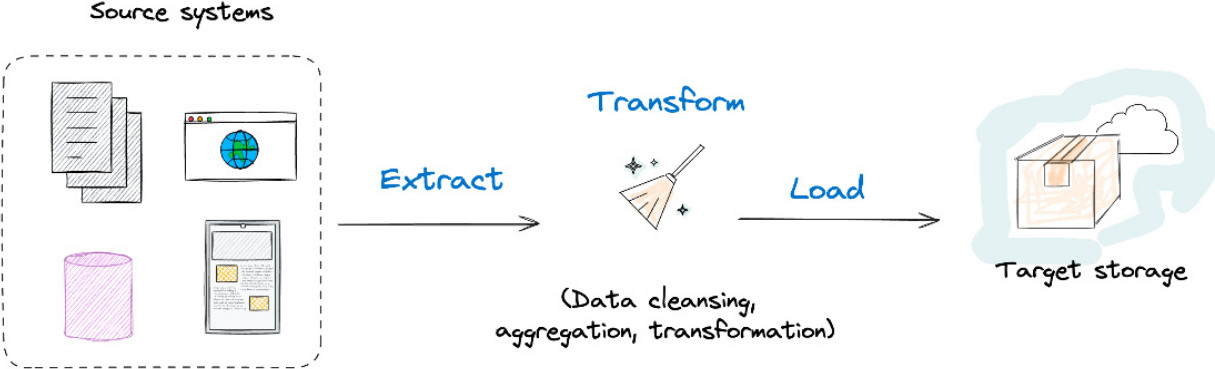
\includegraphics[width=.96\linewidth]{../img/etl.jpg}}
    \vspace{-10pt}
    \normalcolor\caption{ETL-Modell nach \cite[Seite 63]{bonnefoy2024definitive}}
\end{figure}

Für die BfArM-Daten sieht der Integrationsprozess konkret so aus:

\begin{enumerate}
\item \emph{Download:} Die Zip-Dateien werden heruntergeladen. Alternativ kann geprüft werden, ob die Dateien schon lokal vorhanden sind mit einem bestimmten Pfad, der sich nach Kodiersystem und Versionsnummer immer gleich zusammensetzt, zum Beispiel: (Projektverzeichnis)\texttt{/files/icd10gm2024.zip}. Die Download-Funktion sollte die Zip-Dateien ebenfalls unter diesem Pfad abspeichern, falls so gewünscht.
\item \emph{Unzip:} Die Kodes- und Umsteiger-Dateien werden aus der Zip-Datei extrahiert. Normalerweise muss dafür nicht das ganze Archiv in temporäre Dateien entpackt werden -- außer eventuell bei den Versionen 2022, weil das Extrahieren verschachtelter Zip-Dateien eher eine Nischenanwendung ist und nicht unbedingt standardmäßig von Programmiersprachen oder Bibliotheken unterstützt wird. 
\item \emph{Convert Encoding:} Die in ISO-8859-1 kodierten Kodes-Dateien müssen in UTF-8 umgewandelt werden. In \cite{charencoding} werden die beiden Zeichenkodierungen genauer erklärt, aber für die BfArM-Daten ist eigentlich nur relevant, dass Umlaute mit unterschiedlichen Werten kodiert sind. Also würde das Einlesen eines in ISO-8859-1 kodierten Umlauts als UTF-8 ein anderes Zeichen als Resultat ergeben. Die Umsteiger-Dateien sind davon nicht betroffen, weil in diesen keine Umlaute enthalten sind. 
\item \emph{Parse CSV:} Ein Parser wandelt eine Datei in eine Datenstruktur um; für CSV sollte jede Programmiersprache so eine Funktion standardmäßig zur Verfügung stellen. Für die BfArM-Dateien ist das Ergebnis ein zweidimensionales Array mit zwei Spalten für die Kodes, beziehungsweise drei bis sechs Spalten für die Umsteiger je nach Kodiersystem und Version. 
\item \emph{Process Data:} Aufgrund der oben erwähnten Abweichungen ist die Vorverarbeitung der Daten der komplexeste Schritt und wird im nächsten Abschnitt genauer erklärt. Außerdem müssen nicht alle Daten gespeichert werden. Vor allem in Bezug auf die Zip-Dateien ergibt das eine Reduktion der Datenmenge um etwa einen Faktor von zehn. 
\item \emph{Insert:} Die bearbeiteten Daten werden für die Verwendung durch Applikationen gespeichert. Zum Beispiel für eine relationale Datenbank werden pro Dateityp, Kodiersystem und Version eine Tabelle angelegt und die Daten in diese geschrieben. Konkret für SQL müssen außerdem die Hochkommata in den Codes-Dateien beachtet werden. 
\end{enumerate}

\begin{figure}[H]
    \centering\large
    \resizebox{.9\textwidth}{!}{% Graphic for TeX using PGF
% Title: /home/simon/jacuke_ma/tex/dia/data-integration.dia
% Creator: Dia v0.97+git
% CreationDate: Wed Sep 11 07:50:56 2024
% For: simon
% \usepackage{tikz}
% The following commands are not supported in PSTricks at present
% We define them conditionally, so when they are implemented,
% this pgf file will use them.
\ifx\du\undefined
  \newlength{\du}
\fi
\setlength{\du}{15\unitlength}
\begin{tikzpicture}[even odd rule]
\pgftransformxscale{1.000000}
\pgftransformyscale{-1.000000}
\definecolor{dialinecolor}{rgb}{0.000000, 0.000000, 0.000000}
\pgfsetstrokecolor{dialinecolor}
\pgfsetstrokeopacity{1.000000}
\definecolor{diafillcolor}{rgb}{1.000000, 1.000000, 1.000000}
\pgfsetfillcolor{diafillcolor}
\pgfsetfillopacity{1.000000}
\pgfsetlinewidth{0.100000\du}
\pgfsetdash{}{0pt}
\pgfsetmiterjoin
\pgfsetbuttcap
{\pgfsetcornersarced{\pgfpoint{0.000000\du}{0.000000\du}}\definecolor{diafillcolor}{rgb}{1.000000, 1.000000, 1.000000}
\pgfsetfillcolor{diafillcolor}
\pgfsetfillopacity{0.396078}
\fill (19.000000\du,-6.000000\du)--(19.000000\du,22.000000\du)--(52.000000\du,22.000000\du)--(52.000000\du,-6.000000\du)--cycle;
}{\pgfsetcornersarced{\pgfpoint{0.000000\du}{0.000000\du}}\definecolor{dialinecolor}{rgb}{1.000000, 1.000000, 1.000000}
\pgfsetstrokecolor{dialinecolor}
\pgfsetstrokeopacity{1.000000}
\draw (19.000000\du,-6.000000\du)--(19.000000\du,22.000000\du)--(52.000000\du,22.000000\du)--(52.000000\du,-6.000000\du)--cycle;
}\pgfsetlinewidth{0.100000\du}
\pgfsetdash{}{0pt}
\pgfsetbuttcap
\pgfsetmiterjoin
\pgfsetlinewidth{0.001000\du}
\pgfsetbuttcap
\pgfsetmiterjoin
\pgfsetdash{}{0pt}
\definecolor{diafillcolor}{rgb}{0.717647, 0.717647, 0.615686}
\pgfsetfillcolor{diafillcolor}
\pgfsetfillopacity{1.000000}
\pgfpathmoveto{\pgfpoint{21.000000\du}{-3.393141\du}}
\pgfpathlineto{\pgfpoint{21.000000\du}{4.150583\du}}
\pgfpathlineto{\pgfpoint{25.458746\du}{4.150583\du}}
\pgfpathlineto{\pgfpoint{25.458746\du}{-3.393141\du}}
\pgfpathlineto{\pgfpoint{21.000000\du}{-3.393141\du}}
\pgfpathclose
\pgfusepath{fill}
\pgfsetbuttcap
\pgfsetmiterjoin
\pgfsetdash{}{0pt}
\definecolor{dialinecolor}{rgb}{0.286275, 0.286275, 0.211765}
\pgfsetstrokecolor{dialinecolor}
\pgfsetstrokeopacity{1.000000}
\pgfpathmoveto{\pgfpoint{21.000000\du}{-3.393141\du}}
\pgfpathlineto{\pgfpoint{21.000000\du}{4.150583\du}}
\pgfpathlineto{\pgfpoint{25.458746\du}{4.150583\du}}
\pgfpathlineto{\pgfpoint{25.458746\du}{-3.393141\du}}
\pgfpathlineto{\pgfpoint{21.000000\du}{-3.393141\du}}
\pgfusepath{stroke}
\pgfsetbuttcap
\pgfsetmiterjoin
\pgfsetdash{}{0pt}
\definecolor{diafillcolor}{rgb}{0.788235, 0.788235, 0.713726}
\pgfsetfillcolor{diafillcolor}
\pgfsetfillopacity{1.000000}
\pgfpathmoveto{\pgfpoint{21.000000\du}{-3.393141\du}}
\pgfpathlineto{\pgfpoint{21.604191\du}{-4.000000\du}}
\pgfpathlineto{\pgfpoint{26.061604\du}{-4.000000\du}}
\pgfpathlineto{\pgfpoint{25.458746\du}{-3.393141\du}}
\pgfpathlineto{\pgfpoint{21.000000\du}{-3.393141\du}}
\pgfpathclose
\pgfusepath{fill}
\pgfsetbuttcap
\pgfsetmiterjoin
\pgfsetdash{}{0pt}
\definecolor{dialinecolor}{rgb}{0.286275, 0.286275, 0.211765}
\pgfsetstrokecolor{dialinecolor}
\pgfsetstrokeopacity{1.000000}
\pgfpathmoveto{\pgfpoint{21.000000\du}{-3.393141\du}}
\pgfpathlineto{\pgfpoint{21.604191\du}{-4.000000\du}}
\pgfpathlineto{\pgfpoint{26.032261\du}{-4.000000\du}}
\pgfusepath{stroke}
\pgfsetbuttcap
\pgfsetmiterjoin
\pgfsetdash{}{0pt}
\definecolor{dialinecolor}{rgb}{0.286275, 0.286275, 0.211765}
\pgfsetstrokecolor{dialinecolor}
\pgfsetstrokeopacity{1.000000}
\pgfpathmoveto{\pgfpoint{26.032261\du}{-3.969324\du}}
\pgfpathlineto{\pgfpoint{25.458746\du}{-3.393141\du}}
\pgfpathlineto{\pgfpoint{21.000000\du}{-3.393141\du}}
\pgfusepath{stroke}
\pgfsetbuttcap
\pgfsetmiterjoin
\pgfsetdash{}{0pt}
\definecolor{diafillcolor}{rgb}{0.788235, 0.788235, 0.713726}
\pgfsetfillcolor{diafillcolor}
\pgfsetfillopacity{1.000000}
\pgfpathmoveto{\pgfpoint{21.274754\du}{-2.954335\du}}
\pgfpathlineto{\pgfpoint{23.311399\du}{-2.954335\du}}
\pgfpathlineto{\pgfpoint{23.311399\du}{-1.964688\du}}
\pgfpathlineto{\pgfpoint{21.274754\du}{-1.964688\du}}
\pgfpathlineto{\pgfpoint{21.274754\du}{-2.954335\du}}
\pgfpathclose
\pgfusepath{fill}
\pgfsetbuttcap
\pgfsetmiterjoin
\pgfsetdash{}{0pt}
\definecolor{dialinecolor}{rgb}{0.384314, 0.384314, 0.282353}
\pgfsetstrokecolor{dialinecolor}
\pgfsetstrokeopacity{1.000000}
\pgfpathmoveto{\pgfpoint{21.274754\du}{-2.954335\du}}
\pgfpathlineto{\pgfpoint{23.310065\du}{-2.954335\du}}
\pgfpathlineto{\pgfpoint{23.310065\du}{-1.966022\du}}
\pgfpathlineto{\pgfpoint{21.274754\du}{-1.966022\du}}
\pgfpathlineto{\pgfpoint{21.274754\du}{-2.954335\du}}
\pgfusepath{stroke}
\pgfsetlinewidth{0.030000\du}
\pgfsetbuttcap
\pgfsetmiterjoin
\pgfsetdash{}{0pt}
\definecolor{dialinecolor}{rgb}{0.925490, 0.925490, 0.905882}
\pgfsetstrokecolor{dialinecolor}
\pgfsetstrokeopacity{1.000000}
\pgfpathmoveto{\pgfpoint{21.549507\du}{-2.458178\du}}
\pgfpathlineto{\pgfpoint{22.977960\du}{-2.458178\du}}
\pgfusepath{stroke}
\pgfsetlinewidth{0.001000\du}
\pgfsetbuttcap
\pgfsetmiterjoin
\pgfsetdash{}{0pt}
\definecolor{diafillcolor}{rgb}{0.478431, 0.478431, 0.352941}
\pgfsetfillcolor{diafillcolor}
\pgfsetfillopacity{1.000000}
\pgfpathmoveto{\pgfpoint{25.458746\du}{4.150583\du}}
\pgfpathlineto{\pgfpoint{26.061604\du}{3.542390\du}}
\pgfpathlineto{\pgfpoint{26.061604\du}{-4.000000\du}}
\pgfpathlineto{\pgfpoint{25.458746\du}{-3.393141\du}}
\pgfpathlineto{\pgfpoint{25.458746\du}{4.150583\du}}
\pgfpathclose
\pgfusepath{fill}
\pgfsetbuttcap
\pgfsetmiterjoin
\pgfsetdash{}{0pt}
\definecolor{dialinecolor}{rgb}{0.286275, 0.286275, 0.211765}
\pgfsetstrokecolor{dialinecolor}
\pgfsetstrokeopacity{1.000000}
\pgfpathmoveto{\pgfpoint{25.458746\du}{4.150583\du}}
\pgfpathlineto{\pgfpoint{26.032261\du}{3.573067\du}}
\pgfusepath{stroke}
\pgfsetbuttcap
\pgfsetmiterjoin
\pgfsetdash{}{0pt}
\definecolor{dialinecolor}{rgb}{0.286275, 0.286275, 0.211765}
\pgfsetstrokecolor{dialinecolor}
\pgfsetstrokeopacity{1.000000}
\pgfpathmoveto{\pgfpoint{26.032261\du}{-3.969324\du}}
\pgfpathlineto{\pgfpoint{25.458746\du}{-3.393141\du}}
\pgfpathlineto{\pgfpoint{25.458746\du}{4.150583\du}}
\pgfusepath{stroke}
\pgfsetlinewidth{0.030000\du}
\pgfsetbuttcap
\pgfsetmiterjoin
\pgfsetdash{}{0pt}
\definecolor{dialinecolor}{rgb}{0.925490, 0.925490, 0.905882}
\pgfsetstrokecolor{dialinecolor}
\pgfsetstrokeopacity{1.000000}
\pgfpathmoveto{\pgfpoint{21.056018\du}{3.653092\du}}
\pgfpathlineto{\pgfpoint{25.457413\du}{3.653092\du}}
\pgfusepath{stroke}
\pgfsetbuttcap
\pgfsetmiterjoin
\pgfsetdash{}{0pt}
\definecolor{dialinecolor}{rgb}{0.000000, 0.000000, 0.000000}
\pgfsetstrokecolor{dialinecolor}
\pgfsetstrokeopacity{1.000000}
\pgfpathmoveto{\pgfpoint{21.056018\du}{-0.365515\du}}
\pgfpathlineto{\pgfpoint{25.457413\du}{-0.365515\du}}
\pgfusepath{stroke}
\pgfsetbuttcap
\pgfsetmiterjoin
\pgfsetdash{}{0pt}
\definecolor{dialinecolor}{rgb}{0.286275, 0.286275, 0.211765}
\pgfsetstrokecolor{dialinecolor}
\pgfsetstrokeopacity{1.000000}
\pgfpathmoveto{\pgfpoint{21.000000\du}{3.598408\du}}
\pgfpathlineto{\pgfpoint{25.453411\du}{3.598408\du}}
\pgfusepath{stroke}
\pgfsetbuttcap
\pgfsetmiterjoin
\pgfsetdash{}{0pt}
\definecolor{dialinecolor}{rgb}{0.000000, 0.000000, 0.000000}
\pgfsetstrokecolor{dialinecolor}
\pgfsetstrokeopacity{1.000000}
\pgfpathmoveto{\pgfpoint{21.000000\du}{-0.421533\du}}
\pgfpathlineto{\pgfpoint{25.453411\du}{-0.421533\du}}
\pgfusepath{stroke}
\pgfsetlinewidth{0.001000\du}
\pgfsetbuttcap
\pgfsetmiterjoin
\pgfsetdash{}{0pt}
\definecolor{dialinecolor}{rgb}{0.925490, 0.925490, 0.905882}
\pgfsetstrokecolor{dialinecolor}
\pgfsetstrokeopacity{1.000000}
\pgfpathmoveto{\pgfpoint{21.274754\du}{-2.018039\du}}
\pgfpathlineto{\pgfpoint{21.274754\du}{-2.954335\du}}
\pgfpathlineto{\pgfpoint{23.255381\du}{-2.954335\du}}
\pgfusepath{stroke}
\pgfsetlinewidth{0.100000\du}
\pgfsetdash{}{0pt}
\pgfsetbuttcap
\pgfsetmiterjoin
\pgfsetlinewidth{0.001000\du}
\pgfsetbuttcap
\pgfsetmiterjoin
\pgfsetdash{}{0pt}
\definecolor{diafillcolor}{rgb}{0.647059, 0.647059, 0.521569}
\pgfsetfillcolor{diafillcolor}
\pgfsetfillopacity{1.000000}
\pgfpathmoveto{\pgfpoint{51.124567\du}{17.183102\du}}
\pgfpathlineto{\pgfpoint{51.119703\du}{17.120845\du}}
\pgfpathlineto{\pgfpoint{51.106085\du}{17.059561\du}}
\pgfpathlineto{\pgfpoint{51.082738\du}{16.998276\du}}
\pgfpathlineto{\pgfpoint{51.050637\du}{16.937964\du}}
\pgfpathlineto{\pgfpoint{51.010753\du}{16.877653\du}}
\pgfpathlineto{\pgfpoint{50.961142\du}{16.818314\du}}
\pgfpathlineto{\pgfpoint{50.902776\du}{16.759947\du}}
\pgfpathlineto{\pgfpoint{50.835655\du}{16.702554\du}}
\pgfpathlineto{\pgfpoint{50.759778\du}{16.646133\du}}
\pgfpathlineto{\pgfpoint{50.676120\du}{16.592631\du}}
\pgfpathlineto{\pgfpoint{50.584680\du}{16.539129\du}}
\pgfpathlineto{\pgfpoint{50.486430\du}{16.486599\du}}
\pgfpathlineto{\pgfpoint{50.378453\du}{16.436988\du}}
\pgfpathlineto{\pgfpoint{50.264639\du}{16.389322\du}}
\pgfpathlineto{\pgfpoint{50.144015\du}{16.343602\du}}
\pgfpathlineto{\pgfpoint{50.015609\du}{16.299827\du}}
\pgfpathlineto{\pgfpoint{49.882340\du}{16.258971\du}}
\pgfpathlineto{\pgfpoint{49.742261\du}{16.220060\du}}
\pgfpathlineto{\pgfpoint{49.597318\du}{16.184068\du}}
\pgfpathlineto{\pgfpoint{49.445566\du}{16.150021\du}}
\pgfpathlineto{\pgfpoint{49.290896\du}{16.117919\du}}
\pgfpathlineto{\pgfpoint{49.130389\du}{16.089709\du}}
\pgfpathlineto{\pgfpoint{48.965991\du}{16.062471\du}}
\pgfpathlineto{\pgfpoint{48.799647\du}{16.040098\du}}
\pgfpathlineto{\pgfpoint{48.628439\du}{16.020642\du}}
\pgfpathlineto{\pgfpoint{48.454314\du}{16.004105\du}}
\pgfpathlineto{\pgfpoint{48.279215\du}{15.989514\du}}
\pgfpathlineto{\pgfpoint{48.101198\du}{15.979786\du}}
\pgfpathlineto{\pgfpoint{47.922208\du}{15.971031\du}}
\pgfpathlineto{\pgfpoint{47.742246\du}{15.965194\du}}
\pgfpathlineto{\pgfpoint{47.562284\du}{15.965194\du}}
\pgfpathlineto{\pgfpoint{47.562284\du}{15.965194\du}}
\pgfpathlineto{\pgfpoint{47.381348\du}{15.965194\du}}
\pgfpathlineto{\pgfpoint{47.201386\du}{15.971031\du}}
\pgfpathlineto{\pgfpoint{47.022396\du}{15.979786\du}}
\pgfpathlineto{\pgfpoint{46.844379\du}{15.989514\du}}
\pgfpathlineto{\pgfpoint{46.669281\du}{16.004105\du}}
\pgfpathlineto{\pgfpoint{46.495155\du}{16.020642\du}}
\pgfpathlineto{\pgfpoint{46.324920\du}{16.040098\du}}
\pgfpathlineto{\pgfpoint{46.157604\du}{16.062471\du}}
\pgfpathlineto{\pgfpoint{45.993206\du}{16.089709\du}}
\pgfpathlineto{\pgfpoint{45.832699\du}{16.117919\du}}
\pgfpathlineto{\pgfpoint{45.678028\du}{16.150021\du}}
\pgfpathlineto{\pgfpoint{45.527249\du}{16.184068\du}}
\pgfpathlineto{\pgfpoint{45.382306\du}{16.220060\du}}
\pgfpathlineto{\pgfpoint{45.242227\du}{16.258971\du}}
\pgfpathlineto{\pgfpoint{45.107985\du}{16.299827\du}}
\pgfpathlineto{\pgfpoint{44.979579\du}{16.343602\du}}
\pgfpathlineto{\pgfpoint{44.859929\du}{16.389322\du}}
\pgfpathlineto{\pgfpoint{44.745142\du}{16.436988\du}}
\pgfpathlineto{\pgfpoint{44.638137\du}{16.486599\du}}
\pgfpathlineto{\pgfpoint{44.538915\du}{16.539129\du}}
\pgfpathlineto{\pgfpoint{44.447474\du}{16.592631\du}}
\pgfpathlineto{\pgfpoint{44.363816\du}{16.646133\du}}
\pgfpathlineto{\pgfpoint{44.287940\du}{16.702554\du}}
\pgfpathlineto{\pgfpoint{44.220819\du}{16.759947\du}}
\pgfpathlineto{\pgfpoint{44.162453\du}{16.818314\du}}
\pgfpathlineto{\pgfpoint{44.112841\du}{16.877653\du}}
\pgfpathlineto{\pgfpoint{44.072958\du}{16.937964\du}}
\pgfpathlineto{\pgfpoint{44.040856\du}{16.998276\du}}
\pgfpathlineto{\pgfpoint{44.017510\du}{17.059561\du}}
\pgfpathlineto{\pgfpoint{44.004864\du}{17.120845\du}}
\pgfpathlineto{\pgfpoint{44.000000\du}{17.183102\du}}
\pgfpathlineto{\pgfpoint{44.000000\du}{17.183102\du}}
\pgfpathlineto{\pgfpoint{44.004864\du}{17.245360\du}}
\pgfpathlineto{\pgfpoint{44.017510\du}{17.305671\du}}
\pgfpathlineto{\pgfpoint{44.040856\du}{17.367929\du}}
\pgfpathlineto{\pgfpoint{44.072958\du}{17.428240\du}}
\pgfpathlineto{\pgfpoint{44.112841\du}{17.488552\du}}
\pgfpathlineto{\pgfpoint{44.162453\du}{17.547891\du}}
\pgfpathlineto{\pgfpoint{44.220819\du}{17.606257\du}}
\pgfpathlineto{\pgfpoint{44.287940\du}{17.663651\du}}
\pgfpathlineto{\pgfpoint{44.363816\du}{17.719099\du}}
\pgfpathlineto{\pgfpoint{44.447474\du}{17.773574\du}}
\pgfpathlineto{\pgfpoint{44.538915\du}{17.827076\du}}
\pgfpathlineto{\pgfpoint{44.638137\du}{17.879606\du}}
\pgfpathlineto{\pgfpoint{44.745142\du}{17.929217\du}}
\pgfpathlineto{\pgfpoint{44.859929\du}{17.976883\du}}
\pgfpathlineto{\pgfpoint{44.979579\du}{18.022603\du}}
\pgfpathlineto{\pgfpoint{45.107985\du}{18.066378\du}}
\pgfpathlineto{\pgfpoint{45.242227\du}{18.107234\du}}
\pgfpathlineto{\pgfpoint{45.382306\du}{18.146145\du}}
\pgfpathlineto{\pgfpoint{45.527249\du}{18.182137\du}}
\pgfpathlineto{\pgfpoint{45.678028\du}{18.216184\du}}
\pgfpathlineto{\pgfpoint{45.832699\du}{18.248285\du}}
\pgfpathlineto{\pgfpoint{45.993206\du}{18.276496\du}}
\pgfpathlineto{\pgfpoint{46.157604\du}{18.302761\du}}
\pgfpathlineto{\pgfpoint{46.324920\du}{18.326107\du}}
\pgfpathlineto{\pgfpoint{46.495155\du}{18.345562\du}}
\pgfpathlineto{\pgfpoint{46.669281\du}{18.362100\du}}
\pgfpathlineto{\pgfpoint{46.844379\du}{18.375718\du}}
\pgfpathlineto{\pgfpoint{47.022396\du}{18.386419\du}}
\pgfpathlineto{\pgfpoint{47.201386\du}{18.394201\du}}
\pgfpathlineto{\pgfpoint{47.381348\du}{18.400038\du}}
\pgfpathlineto{\pgfpoint{47.562284\du}{18.401010\du}}
\pgfpathlineto{\pgfpoint{47.562284\du}{18.401010\du}}
\pgfpathlineto{\pgfpoint{47.742246\du}{18.400038\du}}
\pgfpathlineto{\pgfpoint{47.922208\du}{18.394201\du}}
\pgfpathlineto{\pgfpoint{48.101198\du}{18.386419\du}}
\pgfpathlineto{\pgfpoint{48.279215\du}{18.375718\du}}
\pgfpathlineto{\pgfpoint{48.454314\du}{18.362100\du}}
\pgfpathlineto{\pgfpoint{48.628439\du}{18.345562\du}}
\pgfpathlineto{\pgfpoint{48.799647\du}{18.326107\du}}
\pgfpathlineto{\pgfpoint{48.965991\du}{18.302761\du}}
\pgfpathlineto{\pgfpoint{49.130389\du}{18.276496\du}}
\pgfpathlineto{\pgfpoint{49.290896\du}{18.248285\du}}
\pgfpathlineto{\pgfpoint{49.445566\du}{18.216184\du}}
\pgfpathlineto{\pgfpoint{49.597318\du}{18.182137\du}}
\pgfpathlineto{\pgfpoint{49.742261\du}{18.146145\du}}
\pgfpathlineto{\pgfpoint{49.882340\du}{18.107234\du}}
\pgfpathlineto{\pgfpoint{50.015609\du}{18.066378\du}}
\pgfpathlineto{\pgfpoint{50.144015\du}{18.022603\du}}
\pgfpathlineto{\pgfpoint{50.264639\du}{17.976883\du}}
\pgfpathlineto{\pgfpoint{50.378453\du}{17.929217\du}}
\pgfpathlineto{\pgfpoint{50.486430\du}{17.879606\du}}
\pgfpathlineto{\pgfpoint{50.584680\du}{17.827076\du}}
\pgfpathlineto{\pgfpoint{50.676120\du}{17.773574\du}}
\pgfpathlineto{\pgfpoint{50.759778\du}{17.719099\du}}
\pgfpathlineto{\pgfpoint{50.835655\du}{17.663651\du}}
\pgfpathlineto{\pgfpoint{50.902776\du}{17.606257\du}}
\pgfpathlineto{\pgfpoint{50.961142\du}{17.547891\du}}
\pgfpathlineto{\pgfpoint{51.010753\du}{17.488552\du}}
\pgfpathlineto{\pgfpoint{51.050637\du}{17.428240\du}}
\pgfpathlineto{\pgfpoint{51.082738\du}{17.367929\du}}
\pgfpathlineto{\pgfpoint{51.106085\du}{17.305671\du}}
\pgfpathlineto{\pgfpoint{51.119703\du}{17.245360\du}}
\pgfpathlineto{\pgfpoint{51.124567\du}{17.183102\du}}
\pgfpathclose
\pgfusepath{fill}
\pgfsetbuttcap
\pgfsetmiterjoin
\pgfsetdash{}{0pt}
\definecolor{dialinecolor}{rgb}{0.286275, 0.286275, 0.211765}
\pgfsetstrokecolor{dialinecolor}
\pgfsetstrokeopacity{1.000000}
\pgfpathmoveto{\pgfpoint{51.082738\du}{17.163647\du}}
\pgfpathlineto{\pgfpoint{51.077874\du}{17.101390\du}}
\pgfpathlineto{\pgfpoint{51.065228\du}{17.042051\du}}
\pgfpathlineto{\pgfpoint{51.042855\du}{16.981739\du}}
\pgfpathlineto{\pgfpoint{51.011726\du}{16.922400\du}}
\pgfpathlineto{\pgfpoint{50.969897\du}{16.862088\du}}
\pgfpathlineto{\pgfpoint{50.919313\du}{16.804695\du}}
\pgfpathlineto{\pgfpoint{50.863865\du}{16.746329\du}}
\pgfpathlineto{\pgfpoint{50.795771\du}{16.691854\du}}
\pgfpathlineto{\pgfpoint{50.720868\du}{16.636406\du}}
\pgfpathlineto{\pgfpoint{50.638182\du}{16.581931\du}}
\pgfpathlineto{\pgfpoint{50.546742\du}{16.530374\du}}
\pgfpathlineto{\pgfpoint{50.448492\du}{16.478817\du}}
\pgfpathlineto{\pgfpoint{50.342460\du}{16.430178\du}}
\pgfpathlineto{\pgfpoint{50.230592\du}{16.381540\du}}
\pgfpathlineto{\pgfpoint{50.108023\du}{16.337765\du}}
\pgfpathlineto{\pgfpoint{49.980590\du}{16.294963\du}}
\pgfpathlineto{\pgfpoint{49.847320\du}{16.254107\du}}
\pgfpathlineto{\pgfpoint{49.709187\du}{16.216169\du}}
\pgfpathlineto{\pgfpoint{49.565217\du}{16.181149\du}}
\pgfpathlineto{\pgfpoint{49.415410\du}{16.147102\du}}
\pgfpathlineto{\pgfpoint{49.259767\du}{16.116947\du}}
\pgfpathlineto{\pgfpoint{49.101206\du}{16.088736\du}}
\pgfpathlineto{\pgfpoint{48.937780\du}{16.062471\du}}
\pgfpathlineto{\pgfpoint{48.772409\du}{16.040098\du}}
\pgfpathlineto{\pgfpoint{48.603147\du}{16.020642\du}}
\pgfpathlineto{\pgfpoint{48.429022\du}{16.005078\du}}
\pgfpathlineto{\pgfpoint{48.254896\du}{15.989514\du}}
\pgfpathlineto{\pgfpoint{48.077852\du}{15.980759\du}}
\pgfpathlineto{\pgfpoint{47.900808\du}{15.972977\du}}
\pgfpathlineto{\pgfpoint{47.719872\du}{15.968113\du}}
\pgfpathlineto{\pgfpoint{47.540883\du}{15.965194\du}}
\pgfpathlineto{\pgfpoint{47.540883\du}{15.965194\du}}
\pgfpathlineto{\pgfpoint{47.361893\du}{15.968113\du}}
\pgfpathlineto{\pgfpoint{47.182903\du}{15.972977\du}}
\pgfpathlineto{\pgfpoint{47.003914\du}{15.980759\du}}
\pgfpathlineto{\pgfpoint{46.828815\du}{15.989514\du}}
\pgfpathlineto{\pgfpoint{46.653716\du}{16.005078\du}}
\pgfpathlineto{\pgfpoint{46.480563\du}{16.020642\du}}
\pgfpathlineto{\pgfpoint{46.310329\du}{16.040098\du}}
\pgfpathlineto{\pgfpoint{46.143985\du}{16.062471\du}}
\pgfpathlineto{\pgfpoint{45.981532\du}{16.088736\du}}
\pgfpathlineto{\pgfpoint{45.822971\du}{16.116947\du}}
\pgfpathlineto{\pgfpoint{45.667328\du}{16.147102\du}}
\pgfpathlineto{\pgfpoint{45.517521\du}{16.181149\du}}
\pgfpathlineto{\pgfpoint{45.374524\du}{16.216169\du}}
\pgfpathlineto{\pgfpoint{45.234445\du}{16.254107\du}}
\pgfpathlineto{\pgfpoint{45.100203\du}{16.294963\du}}
\pgfpathlineto{\pgfpoint{44.973743\du}{16.337765\du}}
\pgfpathlineto{\pgfpoint{44.853119\du}{16.381540\du}}
\pgfpathlineto{\pgfpoint{44.741251\du}{16.430178\du}}
\pgfpathlineto{\pgfpoint{44.634246\du}{16.478817\du}}
\pgfpathlineto{\pgfpoint{44.535023\du}{16.530374\du}}
\pgfpathlineto{\pgfpoint{44.445529\du}{16.581931\du}}
\pgfpathlineto{\pgfpoint{44.362843\du}{16.636406\du}}
\pgfpathlineto{\pgfpoint{44.285994\du}{16.691854\du}}
\pgfpathlineto{\pgfpoint{44.219846\du}{16.746329\du}}
\pgfpathlineto{\pgfpoint{44.162453\du}{16.804695\du}}
\pgfpathlineto{\pgfpoint{44.112841\du}{16.862088\du}}
\pgfpathlineto{\pgfpoint{44.071985\du}{16.922400\du}}
\pgfpathlineto{\pgfpoint{44.039884\du}{16.981739\du}}
\pgfpathlineto{\pgfpoint{44.017510\du}{17.042051\du}}
\pgfpathlineto{\pgfpoint{44.004864\du}{17.101390\du}}
\pgfpathlineto{\pgfpoint{44.000000\du}{17.163647\du}}
\pgfpathlineto{\pgfpoint{44.000000\du}{17.163647\du}}
\pgfpathlineto{\pgfpoint{44.004864\du}{17.223959\du}}
\pgfpathlineto{\pgfpoint{44.017510\du}{17.283298\du}}
\pgfpathlineto{\pgfpoint{44.039884\du}{17.344582\du}}
\pgfpathlineto{\pgfpoint{44.071985\du}{17.403921\du}}
\pgfpathlineto{\pgfpoint{44.112841\du}{17.463260\du}}
\pgfpathlineto{\pgfpoint{44.162453\du}{17.521626\du}}
\pgfpathlineto{\pgfpoint{44.219846\du}{17.579020\du}}
\pgfpathlineto{\pgfpoint{44.285994\du}{17.634468\du}}
\pgfpathlineto{\pgfpoint{44.362843\du}{17.688943\du}}
\pgfpathlineto{\pgfpoint{44.445529\du}{17.744391\du}}
\pgfpathlineto{\pgfpoint{44.535023\du}{17.796920\du}}
\pgfpathlineto{\pgfpoint{44.634246\du}{17.846531\du}}
\pgfpathlineto{\pgfpoint{44.741251\du}{17.896143\du}}
\pgfpathlineto{\pgfpoint{44.853119\du}{17.943808\du}}
\pgfpathlineto{\pgfpoint{44.973743\du}{17.988556\du}}
\pgfpathlineto{\pgfpoint{45.100203\du}{18.031358\du}}
\pgfpathlineto{\pgfpoint{45.234445\du}{18.071241\du}}
\pgfpathlineto{\pgfpoint{45.374524\du}{18.110152\du}}
\pgfpathlineto{\pgfpoint{45.517521\du}{18.145172\du}}
\pgfpathlineto{\pgfpoint{45.667328\du}{18.179219\du}}
\pgfpathlineto{\pgfpoint{45.822971\du}{18.210347\du}}
\pgfpathlineto{\pgfpoint{45.981532\du}{18.237585\du}}
\pgfpathlineto{\pgfpoint{46.143985\du}{18.262877\du}}
\pgfpathlineto{\pgfpoint{46.310329\du}{18.285251\du}}
\pgfpathlineto{\pgfpoint{46.480563\du}{18.304706\du}}
\pgfpathlineto{\pgfpoint{46.653716\du}{18.321243\du}}
\pgfpathlineto{\pgfpoint{46.828815\du}{18.335835\du}}
\pgfpathlineto{\pgfpoint{47.003914\du}{18.345562\du}}
\pgfpathlineto{\pgfpoint{47.182903\du}{18.353345\du}}
\pgfpathlineto{\pgfpoint{47.361893\du}{18.358208\du}}
\pgfpathlineto{\pgfpoint{47.540883\du}{18.360154\du}}
\pgfpathlineto{\pgfpoint{47.540883\du}{18.360154\du}}
\pgfpathlineto{\pgfpoint{47.719872\du}{18.358208\du}}
\pgfpathlineto{\pgfpoint{47.900808\du}{18.353345\du}}
\pgfpathlineto{\pgfpoint{48.077852\du}{18.345562\du}}
\pgfpathlineto{\pgfpoint{48.254896\du}{18.335835\du}}
\pgfpathlineto{\pgfpoint{48.429022\du}{18.321243\du}}
\pgfpathlineto{\pgfpoint{48.603147\du}{18.304706\du}}
\pgfpathlineto{\pgfpoint{48.772409\du}{18.285251\du}}
\pgfpathlineto{\pgfpoint{48.937780\du}{18.262877\du}}
\pgfpathlineto{\pgfpoint{49.101206\du}{18.237585\du}}
\pgfpathlineto{\pgfpoint{49.259767\du}{18.210347\du}}
\pgfpathlineto{\pgfpoint{49.415410\du}{18.179219\du}}
\pgfpathlineto{\pgfpoint{49.565217\du}{18.145172\du}}
\pgfpathlineto{\pgfpoint{49.709187\du}{18.110152\du}}
\pgfpathlineto{\pgfpoint{49.847320\du}{18.071241\du}}
\pgfpathlineto{\pgfpoint{49.980590\du}{18.031358\du}}
\pgfpathlineto{\pgfpoint{50.108023\du}{17.988556\du}}
\pgfpathlineto{\pgfpoint{50.230592\du}{17.943808\du}}
\pgfpathlineto{\pgfpoint{50.342460\du}{17.896143\du}}
\pgfpathlineto{\pgfpoint{50.448492\du}{17.846531\du}}
\pgfpathlineto{\pgfpoint{50.546742\du}{17.796920\du}}
\pgfpathlineto{\pgfpoint{50.638182\du}{17.744391\du}}
\pgfpathlineto{\pgfpoint{50.720868\du}{17.688943\du}}
\pgfpathlineto{\pgfpoint{50.795771\du}{17.634468\du}}
\pgfpathlineto{\pgfpoint{50.863865\du}{17.579020\du}}
\pgfpathlineto{\pgfpoint{50.919313\du}{17.521626\du}}
\pgfpathlineto{\pgfpoint{50.969897\du}{17.463260\du}}
\pgfpathlineto{\pgfpoint{51.011726\du}{17.403921\du}}
\pgfpathlineto{\pgfpoint{51.042855\du}{17.344582\du}}
\pgfpathlineto{\pgfpoint{51.065228\du}{17.283298\du}}
\pgfpathlineto{\pgfpoint{51.077874\du}{17.223959\du}}
\pgfpathlineto{\pgfpoint{51.082738\du}{17.163647\du}}
\pgfusepath{stroke}
\pgfsetbuttcap
\pgfsetmiterjoin
\pgfsetdash{}{0pt}
\definecolor{diafillcolor}{rgb}{0.647059, 0.647059, 0.521569}
\pgfsetfillcolor{diafillcolor}
\pgfsetfillopacity{1.000000}
\pgfpathmoveto{\pgfpoint{44.000000\du}{14.639309\du}}
\pgfpathlineto{\pgfpoint{44.000000\du}{17.204503\du}}
\pgfpathlineto{\pgfpoint{51.082738\du}{17.204503\du}}
\pgfpathlineto{\pgfpoint{51.082738\du}{14.639309\du}}
\pgfpathlineto{\pgfpoint{44.000000\du}{14.639309\du}}
\pgfpathclose
\pgfusepath{fill}
\pgfsetbuttcap
\pgfsetmiterjoin
\pgfsetdash{}{0pt}
\definecolor{diafillcolor}{rgb}{0.788235, 0.788235, 0.713726}
\pgfsetfillcolor{diafillcolor}
\pgfsetfillopacity{1.000000}
\pgfpathmoveto{\pgfpoint{51.124567\du}{14.617908\du}}
\pgfpathlineto{\pgfpoint{51.119703\du}{14.554678\du}}
\pgfpathlineto{\pgfpoint{51.106085\du}{14.493393\du}}
\pgfpathlineto{\pgfpoint{51.082738\du}{14.433082\du}}
\pgfpathlineto{\pgfpoint{51.050637\du}{14.372770\du}}
\pgfpathlineto{\pgfpoint{51.010753\du}{14.311485\du}}
\pgfpathlineto{\pgfpoint{50.961142\du}{14.252146\du}}
\pgfpathlineto{\pgfpoint{50.902776\du}{14.192808\du}}
\pgfpathlineto{\pgfpoint{50.835655\du}{14.137360\du}}
\pgfpathlineto{\pgfpoint{50.759778\du}{14.081912\du}}
\pgfpathlineto{\pgfpoint{50.676120\du}{14.025491\du}}
\pgfpathlineto{\pgfpoint{50.584680\du}{13.973934\du}}
\pgfpathlineto{\pgfpoint{50.486430\du}{13.921405\du}}
\pgfpathlineto{\pgfpoint{50.378453\du}{13.870821\du}}
\pgfpathlineto{\pgfpoint{50.264639\du}{13.824128\du}}
\pgfpathlineto{\pgfpoint{50.144015\du}{13.778408\du}}
\pgfpathlineto{\pgfpoint{50.015609\du}{13.733660\du}}
\pgfpathlineto{\pgfpoint{49.882340\du}{13.692804\du}}
\pgfpathlineto{\pgfpoint{49.742261\du}{13.654866\du}}
\pgfpathlineto{\pgfpoint{49.597318\du}{13.617900\du}}
\pgfpathlineto{\pgfpoint{49.445566\du}{13.583854\du}}
\pgfpathlineto{\pgfpoint{49.290896\du}{13.552725\du}}
\pgfpathlineto{\pgfpoint{49.130389\du}{13.524515\du}}
\pgfpathlineto{\pgfpoint{48.965991\du}{13.498250\du}}
\pgfpathlineto{\pgfpoint{48.799647\du}{13.474903\du}}
\pgfpathlineto{\pgfpoint{48.628439\du}{13.455448\du}}
\pgfpathlineto{\pgfpoint{48.454314\du}{13.438911\du}}
\pgfpathlineto{\pgfpoint{48.279215\du}{13.425292\du}}
\pgfpathlineto{\pgfpoint{48.101198\du}{13.414592\du}}
\pgfpathlineto{\pgfpoint{47.922208\du}{13.405837\du}}
\pgfpathlineto{\pgfpoint{47.742246\du}{13.400973\du}}
\pgfpathlineto{\pgfpoint{47.562284\du}{13.400000\du}}
\pgfpathlineto{\pgfpoint{47.562284\du}{13.400000\du}}
\pgfpathlineto{\pgfpoint{47.381348\du}{13.400973\du}}
\pgfpathlineto{\pgfpoint{47.201386\du}{13.405837\du}}
\pgfpathlineto{\pgfpoint{47.022396\du}{13.414592\du}}
\pgfpathlineto{\pgfpoint{46.844379\du}{13.425292\du}}
\pgfpathlineto{\pgfpoint{46.669281\du}{13.438911\du}}
\pgfpathlineto{\pgfpoint{46.495155\du}{13.455448\du}}
\pgfpathlineto{\pgfpoint{46.324920\du}{13.474903\du}}
\pgfpathlineto{\pgfpoint{46.157604\du}{13.498250\du}}
\pgfpathlineto{\pgfpoint{45.993206\du}{13.524515\du}}
\pgfpathlineto{\pgfpoint{45.832699\du}{13.552725\du}}
\pgfpathlineto{\pgfpoint{45.678028\du}{13.583854\du}}
\pgfpathlineto{\pgfpoint{45.527249\du}{13.617900\du}}
\pgfpathlineto{\pgfpoint{45.382306\du}{13.654866\du}}
\pgfpathlineto{\pgfpoint{45.242227\du}{13.692804\du}}
\pgfpathlineto{\pgfpoint{45.107985\du}{13.733660\du}}
\pgfpathlineto{\pgfpoint{44.979579\du}{13.778408\du}}
\pgfpathlineto{\pgfpoint{44.859929\du}{13.824128\du}}
\pgfpathlineto{\pgfpoint{44.745142\du}{13.870821\du}}
\pgfpathlineto{\pgfpoint{44.638137\du}{13.921405\du}}
\pgfpathlineto{\pgfpoint{44.538915\du}{13.973934\du}}
\pgfpathlineto{\pgfpoint{44.447474\du}{14.025491\du}}
\pgfpathlineto{\pgfpoint{44.363816\du}{14.081912\du}}
\pgfpathlineto{\pgfpoint{44.287940\du}{14.137360\du}}
\pgfpathlineto{\pgfpoint{44.220819\du}{14.192808\du}}
\pgfpathlineto{\pgfpoint{44.162453\du}{14.252146\du}}
\pgfpathlineto{\pgfpoint{44.112841\du}{14.311485\du}}
\pgfpathlineto{\pgfpoint{44.072958\du}{14.372770\du}}
\pgfpathlineto{\pgfpoint{44.040856\du}{14.433082\du}}
\pgfpathlineto{\pgfpoint{44.017510\du}{14.493393\du}}
\pgfpathlineto{\pgfpoint{44.004864\du}{14.554678\du}}
\pgfpathlineto{\pgfpoint{44.000000\du}{14.617908\du}}
\pgfpathlineto{\pgfpoint{44.000000\du}{14.617908\du}}
\pgfpathlineto{\pgfpoint{44.004864\du}{14.679193\du}}
\pgfpathlineto{\pgfpoint{44.017510\du}{14.741450\du}}
\pgfpathlineto{\pgfpoint{44.040856\du}{14.800789\du}}
\pgfpathlineto{\pgfpoint{44.072958\du}{14.863046\du}}
\pgfpathlineto{\pgfpoint{44.112841\du}{14.922385\du}}
\pgfpathlineto{\pgfpoint{44.162453\du}{14.982697\du}}
\pgfpathlineto{\pgfpoint{44.220819\du}{15.041063\du}}
\pgfpathlineto{\pgfpoint{44.287940\du}{15.097484\du}}
\pgfpathlineto{\pgfpoint{44.363816\du}{15.153904\du}}
\pgfpathlineto{\pgfpoint{44.447474\du}{15.208379\du}}
\pgfpathlineto{\pgfpoint{44.538915\du}{15.261882\du}}
\pgfpathlineto{\pgfpoint{44.638137\du}{15.313439\du}}
\pgfpathlineto{\pgfpoint{44.745142\du}{15.363050\du}}
\pgfpathlineto{\pgfpoint{44.859929\du}{15.410716\du}}
\pgfpathlineto{\pgfpoint{44.979579\du}{15.457408\du}}
\pgfpathlineto{\pgfpoint{45.107985\du}{15.500210\du}}
\pgfpathlineto{\pgfpoint{45.242227\du}{15.542039\du}}
\pgfpathlineto{\pgfpoint{45.382306\du}{15.580950\du}}
\pgfpathlineto{\pgfpoint{45.527249\du}{15.616943\du}}
\pgfpathlineto{\pgfpoint{45.678028\du}{15.650990\du}}
\pgfpathlineto{\pgfpoint{45.832699\du}{15.683091\du}}
\pgfpathlineto{\pgfpoint{45.993206\du}{15.710329\du}}
\pgfpathlineto{\pgfpoint{46.157604\du}{15.737566\du}}
\pgfpathlineto{\pgfpoint{46.324920\du}{15.759940\du}}
\pgfpathlineto{\pgfpoint{46.495155\du}{15.779395\du}}
\pgfpathlineto{\pgfpoint{46.669281\du}{15.796905\du}}
\pgfpathlineto{\pgfpoint{46.844379\du}{15.809551\du}}
\pgfpathlineto{\pgfpoint{47.022396\du}{15.821224\du}}
\pgfpathlineto{\pgfpoint{47.201386\du}{15.829007\du}}
\pgfpathlineto{\pgfpoint{47.381348\du}{15.833870\du}}
\pgfpathlineto{\pgfpoint{47.562284\du}{15.835816\du}}
\pgfpathlineto{\pgfpoint{47.562284\du}{15.835816\du}}
\pgfpathlineto{\pgfpoint{47.742246\du}{15.833870\du}}
\pgfpathlineto{\pgfpoint{47.922208\du}{15.829007\du}}
\pgfpathlineto{\pgfpoint{48.101198\du}{15.821224\du}}
\pgfpathlineto{\pgfpoint{48.279215\du}{15.809551\du}}
\pgfpathlineto{\pgfpoint{48.454314\du}{15.796905\du}}
\pgfpathlineto{\pgfpoint{48.628439\du}{15.779395\du}}
\pgfpathlineto{\pgfpoint{48.799647\du}{15.759940\du}}
\pgfpathlineto{\pgfpoint{48.965991\du}{15.737566\du}}
\pgfpathlineto{\pgfpoint{49.130389\du}{15.710329\du}}
\pgfpathlineto{\pgfpoint{49.290896\du}{15.683091\du}}
\pgfpathlineto{\pgfpoint{49.445566\du}{15.650990\du}}
\pgfpathlineto{\pgfpoint{49.597318\du}{15.616943\du}}
\pgfpathlineto{\pgfpoint{49.742261\du}{15.580950\du}}
\pgfpathlineto{\pgfpoint{49.882340\du}{15.542039\du}}
\pgfpathlineto{\pgfpoint{50.015609\du}{15.500210\du}}
\pgfpathlineto{\pgfpoint{50.144015\du}{15.457408\du}}
\pgfpathlineto{\pgfpoint{50.264639\du}{15.410716\du}}
\pgfpathlineto{\pgfpoint{50.378453\du}{15.363050\du}}
\pgfpathlineto{\pgfpoint{50.486430\du}{15.313439\du}}
\pgfpathlineto{\pgfpoint{50.584680\du}{15.261882\du}}
\pgfpathlineto{\pgfpoint{50.676120\du}{15.208379\du}}
\pgfpathlineto{\pgfpoint{50.759778\du}{15.153904\du}}
\pgfpathlineto{\pgfpoint{50.835655\du}{15.097484\du}}
\pgfpathlineto{\pgfpoint{50.902776\du}{15.041063\du}}
\pgfpathlineto{\pgfpoint{50.961142\du}{14.982697\du}}
\pgfpathlineto{\pgfpoint{51.010753\du}{14.922385\du}}
\pgfpathlineto{\pgfpoint{51.050637\du}{14.863046\du}}
\pgfpathlineto{\pgfpoint{51.082738\du}{14.800789\du}}
\pgfpathlineto{\pgfpoint{51.106085\du}{14.741450\du}}
\pgfpathlineto{\pgfpoint{51.119703\du}{14.679193\du}}
\pgfpathlineto{\pgfpoint{51.124567\du}{14.617908\du}}
\pgfpathclose
\pgfusepath{fill}
\pgfsetbuttcap
\pgfsetmiterjoin
\pgfsetdash{}{0pt}
\definecolor{dialinecolor}{rgb}{0.286275, 0.286275, 0.211765}
\pgfsetstrokecolor{dialinecolor}
\pgfsetstrokeopacity{1.000000}
\pgfpathmoveto{\pgfpoint{51.082738\du}{14.598453\du}}
\pgfpathlineto{\pgfpoint{51.077874\du}{14.536195\du}}
\pgfpathlineto{\pgfpoint{51.065228\du}{14.476856\du}}
\pgfpathlineto{\pgfpoint{51.042855\du}{14.417517\du}}
\pgfpathlineto{\pgfpoint{51.011726\du}{14.357206\du}}
\pgfpathlineto{\pgfpoint{50.969897\du}{14.295921\du}}
\pgfpathlineto{\pgfpoint{50.919313\du}{14.238528\du}}
\pgfpathlineto{\pgfpoint{50.863865\du}{14.183080\du}}
\pgfpathlineto{\pgfpoint{50.795771\du}{14.125686\du}}
\pgfpathlineto{\pgfpoint{50.720868\du}{14.071211\du}}
\pgfpathlineto{\pgfpoint{50.638182\du}{14.015763\du}}
\pgfpathlineto{\pgfpoint{50.546742\du}{13.965179\du}}
\pgfpathlineto{\pgfpoint{50.448492\du}{13.913623\du}}
\pgfpathlineto{\pgfpoint{50.342460\du}{13.864011\du}}
\pgfpathlineto{\pgfpoint{50.230592\du}{13.818291\du}}
\pgfpathlineto{\pgfpoint{50.108023\du}{13.772571\du}}
\pgfpathlineto{\pgfpoint{49.980590\du}{13.730742\du}}
\pgfpathlineto{\pgfpoint{49.847320\du}{13.689885\du}}
\pgfpathlineto{\pgfpoint{49.709187\du}{13.650975\du}}
\pgfpathlineto{\pgfpoint{49.565217\du}{13.614982\du}}
\pgfpathlineto{\pgfpoint{49.415410\du}{13.581908\du}}
\pgfpathlineto{\pgfpoint{49.259767\du}{13.551752\du}}
\pgfpathlineto{\pgfpoint{49.101206\du}{13.523542\du}}
\pgfpathlineto{\pgfpoint{48.937780\du}{13.498250\du}}
\pgfpathlineto{\pgfpoint{48.772409\du}{13.474903\du}}
\pgfpathlineto{\pgfpoint{48.603147\du}{13.455448\du}}
\pgfpathlineto{\pgfpoint{48.429022\du}{13.438911\du}}
\pgfpathlineto{\pgfpoint{48.254896\du}{13.425292\du}}
\pgfpathlineto{\pgfpoint{48.077852\du}{13.414592\du}}
\pgfpathlineto{\pgfpoint{48.018513\du}{13.411673\du}}
\pgfpathlineto{\pgfpoint{47.063253\du}{13.411673\du}}
\pgfpathlineto{\pgfpoint{47.003914\du}{13.414592\du}}
\pgfpathlineto{\pgfpoint{46.828815\du}{13.425292\du}}
\pgfpathlineto{\pgfpoint{46.653716\du}{13.438911\du}}
\pgfpathlineto{\pgfpoint{46.480563\du}{13.455448\du}}
\pgfpathlineto{\pgfpoint{46.310329\du}{13.474903\du}}
\pgfpathlineto{\pgfpoint{46.143985\du}{13.498250\du}}
\pgfpathlineto{\pgfpoint{45.981532\du}{13.523542\du}}
\pgfpathlineto{\pgfpoint{45.822971\du}{13.551752\du}}
\pgfpathlineto{\pgfpoint{45.667328\du}{13.581908\du}}
\pgfpathlineto{\pgfpoint{45.517521\du}{13.614982\du}}
\pgfpathlineto{\pgfpoint{45.374524\du}{13.650975\du}}
\pgfpathlineto{\pgfpoint{45.234445\du}{13.689885\du}}
\pgfpathlineto{\pgfpoint{45.100203\du}{13.730742\du}}
\pgfpathlineto{\pgfpoint{44.973743\du}{13.772571\du}}
\pgfpathlineto{\pgfpoint{44.853119\du}{13.818291\du}}
\pgfpathlineto{\pgfpoint{44.741251\du}{13.864011\du}}
\pgfpathlineto{\pgfpoint{44.634246\du}{13.913623\du}}
\pgfpathlineto{\pgfpoint{44.535023\du}{13.965179\du}}
\pgfpathlineto{\pgfpoint{44.445529\du}{14.015763\du}}
\pgfpathlineto{\pgfpoint{44.362843\du}{14.071211\du}}
\pgfpathlineto{\pgfpoint{44.285994\du}{14.125686\du}}
\pgfpathlineto{\pgfpoint{44.219846\du}{14.183080\du}}
\pgfpathlineto{\pgfpoint{44.162453\du}{14.238528\du}}
\pgfpathlineto{\pgfpoint{44.112841\du}{14.295921\du}}
\pgfpathlineto{\pgfpoint{44.071985\du}{14.357206\du}}
\pgfpathlineto{\pgfpoint{44.039884\du}{14.417517\du}}
\pgfpathlineto{\pgfpoint{44.017510\du}{14.476856\du}}
\pgfpathlineto{\pgfpoint{44.004864\du}{14.536195\du}}
\pgfpathlineto{\pgfpoint{44.000000\du}{14.598453\du}}
\pgfpathlineto{\pgfpoint{44.000000\du}{14.598453\du}}
\pgfpathlineto{\pgfpoint{44.004864\du}{14.657792\du}}
\pgfpathlineto{\pgfpoint{44.017510\du}{14.719076\du}}
\pgfpathlineto{\pgfpoint{44.039884\du}{14.779388\du}}
\pgfpathlineto{\pgfpoint{44.071985\du}{14.838727\du}}
\pgfpathlineto{\pgfpoint{44.112841\du}{14.898066\du}}
\pgfpathlineto{\pgfpoint{44.162453\du}{14.956432\du}}
\pgfpathlineto{\pgfpoint{44.219846\du}{15.012853\du}}
\pgfpathlineto{\pgfpoint{44.285994\du}{15.070246\du}}
\pgfpathlineto{\pgfpoint{44.362843\du}{15.124721\du}}
\pgfpathlineto{\pgfpoint{44.445529\du}{15.179196\du}}
\pgfpathlineto{\pgfpoint{44.535023\du}{15.231726\du}}
\pgfpathlineto{\pgfpoint{44.634246\du}{15.281337\du}}
\pgfpathlineto{\pgfpoint{44.741251\du}{15.329976\du}}
\pgfpathlineto{\pgfpoint{44.853119\du}{15.378614\du}}
\pgfpathlineto{\pgfpoint{44.973743\du}{15.423362\du}}
\pgfpathlineto{\pgfpoint{45.100203\du}{15.465191\du}}
\pgfpathlineto{\pgfpoint{45.234445\du}{15.505074\du}}
\pgfpathlineto{\pgfpoint{45.374524\du}{15.543985\du}}
\pgfpathlineto{\pgfpoint{45.517521\du}{15.579005\du}}
\pgfpathlineto{\pgfpoint{45.667328\du}{15.613052\du}}
\pgfpathlineto{\pgfpoint{45.822971\du}{15.645153\du}}
\pgfpathlineto{\pgfpoint{45.981532\du}{15.670445\du}}
\pgfpathlineto{\pgfpoint{46.143985\du}{15.697683\du}}
\pgfpathlineto{\pgfpoint{46.310329\du}{15.719084\du}}
\pgfpathlineto{\pgfpoint{46.480563\du}{15.739512\du}}
\pgfpathlineto{\pgfpoint{46.653716\du}{15.757022\du}}
\pgfpathlineto{\pgfpoint{46.828815\du}{15.770640\du}}
\pgfpathlineto{\pgfpoint{47.003914\du}{15.781341\du}}
\pgfpathlineto{\pgfpoint{47.182903\du}{15.788150\du}}
\pgfpathlineto{\pgfpoint{47.361893\du}{15.792041\du}}
\pgfpathlineto{\pgfpoint{47.540883\du}{15.794960\du}}
\pgfpathlineto{\pgfpoint{47.540883\du}{15.794960\du}}
\pgfpathlineto{\pgfpoint{47.719872\du}{15.792041\du}}
\pgfpathlineto{\pgfpoint{47.900808\du}{15.788150\du}}
\pgfpathlineto{\pgfpoint{48.077852\du}{15.781341\du}}
\pgfpathlineto{\pgfpoint{48.254896\du}{15.770640\du}}
\pgfpathlineto{\pgfpoint{48.429022\du}{15.757022\du}}
\pgfpathlineto{\pgfpoint{48.603147\du}{15.739512\du}}
\pgfpathlineto{\pgfpoint{48.772409\du}{15.719084\du}}
\pgfpathlineto{\pgfpoint{48.937780\du}{15.697683\du}}
\pgfpathlineto{\pgfpoint{49.101206\du}{15.670445\du}}
\pgfpathlineto{\pgfpoint{49.259767\du}{15.645153\du}}
\pgfpathlineto{\pgfpoint{49.415410\du}{15.613052\du}}
\pgfpathlineto{\pgfpoint{49.565217\du}{15.579005\du}}
\pgfpathlineto{\pgfpoint{49.709187\du}{15.543985\du}}
\pgfpathlineto{\pgfpoint{49.847320\du}{15.505074\du}}
\pgfpathlineto{\pgfpoint{49.980590\du}{15.465191\du}}
\pgfpathlineto{\pgfpoint{50.108023\du}{15.423362\du}}
\pgfpathlineto{\pgfpoint{50.230592\du}{15.378614\du}}
\pgfpathlineto{\pgfpoint{50.342460\du}{15.329976\du}}
\pgfpathlineto{\pgfpoint{50.448492\du}{15.281337\du}}
\pgfpathlineto{\pgfpoint{50.546742\du}{15.231726\du}}
\pgfpathlineto{\pgfpoint{50.638182\du}{15.179196\du}}
\pgfpathlineto{\pgfpoint{50.720868\du}{15.124721\du}}
\pgfpathlineto{\pgfpoint{50.795771\du}{15.070246\du}}
\pgfpathlineto{\pgfpoint{50.863865\du}{15.012853\du}}
\pgfpathlineto{\pgfpoint{50.919313\du}{14.956432\du}}
\pgfpathlineto{\pgfpoint{50.969897\du}{14.898066\du}}
\pgfpathlineto{\pgfpoint{51.011726\du}{14.838727\du}}
\pgfpathlineto{\pgfpoint{51.042855\du}{14.779388\du}}
\pgfpathlineto{\pgfpoint{51.065228\du}{14.719076\du}}
\pgfpathlineto{\pgfpoint{51.077874\du}{14.657792\du}}
\pgfpathlineto{\pgfpoint{51.082738\du}{14.598453\du}}
\pgfusepath{stroke}
\pgfsetbuttcap
\pgfsetmiterjoin
\pgfsetdash{}{0pt}
\definecolor{dialinecolor}{rgb}{0.000000, 0.000000, 0.000000}
\pgfsetstrokecolor{dialinecolor}
\pgfsetstrokeopacity{1.000000}
\pgfpathmoveto{\pgfpoint{44.000000\du}{14.598453\du}}
\pgfpathlineto{\pgfpoint{44.000000\du}{17.161701\du}}
\pgfusepath{stroke}
\pgfsetbuttcap
\pgfsetmiterjoin
\pgfsetdash{}{0pt}
\definecolor{dialinecolor}{rgb}{0.000000, 0.000000, 0.000000}
\pgfsetstrokecolor{dialinecolor}
\pgfsetstrokeopacity{1.000000}
\pgfpathmoveto{\pgfpoint{51.082738\du}{14.598453\du}}
\pgfpathlineto{\pgfpoint{51.082738\du}{17.161701\du}}
\pgfusepath{stroke}
\pgfsetlinewidth{0.100000\du}
\pgfsetdash{}{0pt}
\pgfsetmiterjoin
\pgfsetbuttcap
{\pgfsetcornersarced{\pgfpoint{0.000000\du}{0.000000\du}}\definecolor{diafillcolor}{rgb}{1.000000, 1.000000, 1.000000}
\pgfsetfillcolor{diafillcolor}
\pgfsetfillopacity{1.000000}
\fill (31.000000\du,-3.000000\du)--(31.000000\du,-1.000000\du)--(39.000000\du,-1.000000\du)--(39.000000\du,-3.000000\du)--cycle;
}{\pgfsetcornersarced{\pgfpoint{0.000000\du}{0.000000\du}}\definecolor{dialinecolor}{rgb}{0.000000, 0.000000, 0.000000}
\pgfsetstrokecolor{dialinecolor}
\pgfsetstrokeopacity{1.000000}
\draw (31.000000\du,-3.000000\du)--(31.000000\du,-1.000000\du)--(39.000000\du,-1.000000\du)--(39.000000\du,-3.000000\du)--cycle;
}% setfont left to latex
\definecolor{dialinecolor}{rgb}{0.000000, 0.000000, 0.000000}
\pgfsetstrokecolor{dialinecolor}
\pgfsetstrokeopacity{1.000000}
\definecolor{diafillcolor}{rgb}{0.000000, 0.000000, 0.000000}
\pgfsetfillcolor{diafillcolor}
\pgfsetfillopacity{1.000000}
\node[anchor=base,inner sep=0pt, outer sep=0pt,color=dialinecolor] at (35.000000\du,-1.652832\du){Download};
\pgfsetlinewidth{0.100000\du}
\pgfsetdash{}{0pt}
\pgfsetmiterjoin
\pgfsetbuttcap
{\pgfsetcornersarced{\pgfpoint{0.000000\du}{0.000000\du}}\definecolor{diafillcolor}{rgb}{1.000000, 1.000000, 1.000000}
\pgfsetfillcolor{diafillcolor}
\pgfsetfillopacity{1.000000}
\fill (31.000000\du,1.000000\du)--(31.000000\du,3.000000\du)--(39.000000\du,3.000000\du)--(39.000000\du,1.000000\du)--cycle;
}{\pgfsetcornersarced{\pgfpoint{0.000000\du}{0.000000\du}}\definecolor{dialinecolor}{rgb}{0.000000, 0.000000, 0.000000}
\pgfsetstrokecolor{dialinecolor}
\pgfsetstrokeopacity{1.000000}
\draw (31.000000\du,1.000000\du)--(31.000000\du,3.000000\du)--(39.000000\du,3.000000\du)--(39.000000\du,1.000000\du)--cycle;
}% setfont left to latex
\definecolor{dialinecolor}{rgb}{0.000000, 0.000000, 0.000000}
\pgfsetstrokecolor{dialinecolor}
\pgfsetstrokeopacity{1.000000}
\definecolor{diafillcolor}{rgb}{0.000000, 0.000000, 0.000000}
\pgfsetfillcolor{diafillcolor}
\pgfsetfillopacity{1.000000}
\node[anchor=base,inner sep=0pt, outer sep=0pt,color=dialinecolor] at (35.000000\du,2.347168\du){Unzip};
\pgfsetlinewidth{0.100000\du}
\pgfsetdash{}{0pt}
\pgfsetmiterjoin
\pgfsetbuttcap
{\pgfsetcornersarced{\pgfpoint{0.000000\du}{0.000000\du}}\definecolor{diafillcolor}{rgb}{1.000000, 1.000000, 1.000000}
\pgfsetfillcolor{diafillcolor}
\pgfsetfillopacity{1.000000}
\fill (31.000000\du,5.000000\du)--(31.000000\du,7.000000\du)--(39.000000\du,7.000000\du)--(39.000000\du,5.000000\du)--cycle;
}{\pgfsetcornersarced{\pgfpoint{0.000000\du}{0.000000\du}}\definecolor{dialinecolor}{rgb}{0.000000, 0.000000, 0.000000}
\pgfsetstrokecolor{dialinecolor}
\pgfsetstrokeopacity{1.000000}
\draw (31.000000\du,5.000000\du)--(31.000000\du,7.000000\du)--(39.000000\du,7.000000\du)--(39.000000\du,5.000000\du)--cycle;
}% setfont left to latex
\definecolor{dialinecolor}{rgb}{0.000000, 0.000000, 0.000000}
\pgfsetstrokecolor{dialinecolor}
\pgfsetstrokeopacity{1.000000}
\definecolor{diafillcolor}{rgb}{0.000000, 0.000000, 0.000000}
\pgfsetfillcolor{diafillcolor}
\pgfsetfillopacity{1.000000}
\node[anchor=base,inner sep=0pt, outer sep=0pt,color=dialinecolor] at (35.000000\du,6.347168\du){Convert Encoding};
\pgfsetlinewidth{0.100000\du}
\pgfsetdash{}{0pt}
\pgfsetmiterjoin
\pgfsetbuttcap
{\pgfsetcornersarced{\pgfpoint{0.000000\du}{0.000000\du}}\definecolor{diafillcolor}{rgb}{1.000000, 1.000000, 1.000000}
\pgfsetfillcolor{diafillcolor}
\pgfsetfillopacity{1.000000}
\fill (31.000000\du,9.000000\du)--(31.000000\du,11.000000\du)--(39.000000\du,11.000000\du)--(39.000000\du,9.000000\du)--cycle;
}{\pgfsetcornersarced{\pgfpoint{0.000000\du}{0.000000\du}}\definecolor{dialinecolor}{rgb}{0.000000, 0.000000, 0.000000}
\pgfsetstrokecolor{dialinecolor}
\pgfsetstrokeopacity{1.000000}
\draw (31.000000\du,9.000000\du)--(31.000000\du,11.000000\du)--(39.000000\du,11.000000\du)--(39.000000\du,9.000000\du)--cycle;
}\pgfsetlinewidth{0.100000\du}
\pgfsetdash{}{0pt}
\pgfsetmiterjoin
\pgfsetbuttcap
{\pgfsetcornersarced{\pgfpoint{0.000000\du}{0.000000\du}}\definecolor{diafillcolor}{rgb}{1.000000, 1.000000, 1.000000}
\pgfsetfillcolor{diafillcolor}
\pgfsetfillopacity{1.000000}
\fill (31.000000\du,13.000000\du)--(31.000000\du,15.000000\du)--(39.000000\du,15.000000\du)--(39.000000\du,13.000000\du)--cycle;
}{\pgfsetcornersarced{\pgfpoint{0.000000\du}{0.000000\du}}\definecolor{dialinecolor}{rgb}{0.000000, 0.000000, 0.000000}
\pgfsetstrokecolor{dialinecolor}
\pgfsetstrokeopacity{1.000000}
\draw (31.000000\du,13.000000\du)--(31.000000\du,15.000000\du)--(39.000000\du,15.000000\du)--(39.000000\du,13.000000\du)--cycle;
}\pgfsetlinewidth{0.100000\du}
\pgfsetdash{}{0pt}
\pgfsetmiterjoin
\pgfsetbuttcap
{\pgfsetcornersarced{\pgfpoint{0.000000\du}{0.000000\du}}\definecolor{diafillcolor}{rgb}{1.000000, 1.000000, 1.000000}
\pgfsetfillcolor{diafillcolor}
\pgfsetfillopacity{1.000000}
\fill (31.000000\du,17.000000\du)--(31.000000\du,19.000000\du)--(39.000000\du,19.000000\du)--(39.000000\du,17.000000\du)--cycle;
}{\pgfsetcornersarced{\pgfpoint{0.000000\du}{0.000000\du}}\definecolor{dialinecolor}{rgb}{0.000000, 0.000000, 0.000000}
\pgfsetstrokecolor{dialinecolor}
\pgfsetstrokeopacity{1.000000}
\draw (31.000000\du,17.000000\du)--(31.000000\du,19.000000\du)--(39.000000\du,19.000000\du)--(39.000000\du,17.000000\du)--cycle;
}\pgfsetlinewidth{0.100000\du}
\pgfsetdash{}{0pt}
\pgfsetbuttcap
{
\definecolor{diafillcolor}{rgb}{0.000000, 0.000000, 0.000000}
\pgfsetfillcolor{diafillcolor}
\pgfsetfillopacity{1.000000}
% was here!!!
\pgfsetarrowsend{stealth}
\definecolor{dialinecolor}{rgb}{0.000000, 0.000000, 0.000000}
\pgfsetstrokecolor{dialinecolor}
\pgfsetstrokeopacity{1.000000}
\draw (35.000000\du,-1.000000\du)--(35.000000\du,1.000000\du);
}
\pgfsetlinewidth{0.100000\du}
\pgfsetdash{}{0pt}
\pgfsetbuttcap
{
\definecolor{diafillcolor}{rgb}{0.000000, 0.000000, 0.000000}
\pgfsetfillcolor{diafillcolor}
\pgfsetfillopacity{1.000000}
% was here!!!
\pgfsetarrowsend{stealth}
\definecolor{dialinecolor}{rgb}{0.000000, 0.000000, 0.000000}
\pgfsetstrokecolor{dialinecolor}
\pgfsetstrokeopacity{1.000000}
\draw (35.000000\du,3.000000\du)--(35.000000\du,5.000000\du);
}
\pgfsetlinewidth{0.100000\du}
\pgfsetdash{}{0pt}
\pgfsetbuttcap
{
\definecolor{diafillcolor}{rgb}{0.000000, 0.000000, 0.000000}
\pgfsetfillcolor{diafillcolor}
\pgfsetfillopacity{1.000000}
% was here!!!
\pgfsetarrowsend{stealth}
\definecolor{dialinecolor}{rgb}{0.000000, 0.000000, 0.000000}
\pgfsetstrokecolor{dialinecolor}
\pgfsetstrokeopacity{1.000000}
\draw (35.000000\du,7.000000\du)--(35.000000\du,9.000000\du);
}
\pgfsetlinewidth{0.100000\du}
\pgfsetdash{}{0pt}
\pgfsetbuttcap
{
\definecolor{diafillcolor}{rgb}{0.000000, 0.000000, 0.000000}
\pgfsetfillcolor{diafillcolor}
\pgfsetfillopacity{1.000000}
% was here!!!
\pgfsetarrowsend{stealth}
\definecolor{dialinecolor}{rgb}{0.000000, 0.000000, 0.000000}
\pgfsetstrokecolor{dialinecolor}
\pgfsetstrokeopacity{1.000000}
\draw (35.000000\du,11.000000\du)--(35.000000\du,13.000000\du);
}
\pgfsetlinewidth{0.100000\du}
\pgfsetdash{}{0pt}
\pgfsetbuttcap
{
\definecolor{diafillcolor}{rgb}{0.000000, 0.000000, 0.000000}
\pgfsetfillcolor{diafillcolor}
\pgfsetfillopacity{1.000000}
% was here!!!
\pgfsetarrowsend{stealth}
\definecolor{dialinecolor}{rgb}{0.000000, 0.000000, 0.000000}
\pgfsetstrokecolor{dialinecolor}
\pgfsetstrokeopacity{1.000000}
\draw (35.000000\du,15.000000\du)--(35.000000\du,17.000000\du);
}
% setfont left to latex
\definecolor{dialinecolor}{rgb}{0.000000, 0.000000, 0.000000}
\pgfsetstrokecolor{dialinecolor}
\pgfsetstrokeopacity{1.000000}
\definecolor{diafillcolor}{rgb}{0.000000, 0.000000, 0.000000}
\pgfsetfillcolor{diafillcolor}
\pgfsetfillopacity{1.000000}
\node[anchor=base,inner sep=0pt, outer sep=0pt,color=dialinecolor] at (35.000000\du,10.347168\du){Parse CSV};
% setfont left to latex
\definecolor{dialinecolor}{rgb}{0.000000, 0.000000, 0.000000}
\pgfsetstrokecolor{dialinecolor}
\pgfsetstrokeopacity{1.000000}
\definecolor{diafillcolor}{rgb}{0.000000, 0.000000, 0.000000}
\pgfsetfillcolor{diafillcolor}
\pgfsetfillopacity{1.000000}
\node[anchor=base,inner sep=0pt, outer sep=0pt,color=dialinecolor] at (35.000000\du,14.347168\du){Process Data};
% setfont left to latex
\definecolor{dialinecolor}{rgb}{0.000000, 0.000000, 0.000000}
\pgfsetstrokecolor{dialinecolor}
\pgfsetstrokeopacity{1.000000}
\definecolor{diafillcolor}{rgb}{0.000000, 0.000000, 0.000000}
\pgfsetfillcolor{diafillcolor}
\pgfsetfillopacity{1.000000}
\node[anchor=base,inner sep=0pt, outer sep=0pt,color=dialinecolor] at (35.000000\du,18.347168\du){Insert};
\pgfsetlinewidth{0.100000\du}
\pgfsetdash{}{0pt}
\pgfsetmiterjoin
\pgfsetbuttcap
{
\definecolor{diafillcolor}{rgb}{0.000000, 0.000000, 0.000000}
\pgfsetfillcolor{diafillcolor}
\pgfsetfillopacity{1.000000}
% was here!!!
\pgfsetarrowsend{stealth}
{\pgfsetcornersarced{\pgfpoint{0.000000\du}{0.000000\du}}\definecolor{dialinecolor}{rgb}{0.000000, 0.000000, 0.000000}
\pgfsetstrokecolor{dialinecolor}
\pgfsetstrokeopacity{1.000000}
\draw (26.062152\du,0.079693\du)--(28.531076\du,0.079693\du)--(28.531076\du,-2.000000\du)--(31.000000\du,-2.000000\du);
}}
\pgfsetlinewidth{0.100000\du}
\pgfsetdash{}{0pt}
\pgfsetmiterjoin
\pgfsetbuttcap
{
\definecolor{diafillcolor}{rgb}{0.000000, 0.000000, 0.000000}
\pgfsetfillcolor{diafillcolor}
\pgfsetfillopacity{1.000000}
% was here!!!
\pgfsetarrowsend{stealth}
{\pgfsetcornersarced{\pgfpoint{0.000000\du}{0.000000\du}}\definecolor{dialinecolor}{rgb}{0.000000, 0.000000, 0.000000}
\pgfsetstrokecolor{dialinecolor}
\pgfsetstrokeopacity{1.000000}
\draw (39.000000\du,18.000000\du)--(41.500000\du,18.000000\du)--(41.500000\du,15.892237\du)--(44.000000\du,15.892237\du);
}}
% setfont left to latex
\definecolor{dialinecolor}{rgb}{0.000000, 0.000000, 0.000000}
\pgfsetstrokecolor{dialinecolor}
\pgfsetstrokeopacity{1.000000}
\definecolor{diafillcolor}{rgb}{0.000000, 0.000000, 0.000000}
\pgfsetfillcolor{diafillcolor}
\pgfsetfillopacity{1.000000}
\node[anchor=base,inner sep=0pt, outer sep=0pt,color=dialinecolor] at (23.228706\du,5.497605\du){BfArM};
% setfont left to latex
\definecolor{dialinecolor}{rgb}{0.000000, 0.000000, 0.000000}
\pgfsetstrokecolor{dialinecolor}
\pgfsetstrokeopacity{1.000000}
\definecolor{diafillcolor}{rgb}{0.000000, 0.000000, 0.000000}
\pgfsetfillcolor{diafillcolor}
\pgfsetfillopacity{1.000000}
\node[anchor=base,inner sep=0pt, outer sep=0pt,color=dialinecolor] at (23.228706\du,6.661772\du){File-Server};
% setfont left to latex
\definecolor{dialinecolor}{rgb}{0.000000, 0.000000, 0.000000}
\pgfsetstrokecolor{dialinecolor}
\pgfsetstrokeopacity{1.000000}
\definecolor{diafillcolor}{rgb}{0.000000, 0.000000, 0.000000}
\pgfsetfillcolor{diafillcolor}
\pgfsetfillopacity{1.000000}
\node[anchor=base,inner sep=0pt, outer sep=0pt,color=dialinecolor] at (47.562284\du,19.748032\du){Application Data};
% setfont left to latex
\definecolor{dialinecolor}{rgb}{0.000000, 0.000000, 0.000000}
\pgfsetstrokecolor{dialinecolor}
\pgfsetstrokeopacity{1.000000}
\definecolor{diafillcolor}{rgb}{0.000000, 0.000000, 0.000000}
\pgfsetfillcolor{diafillcolor}
\pgfsetfillopacity{1.000000}
\node[anchor=base,inner sep=0pt, outer sep=0pt,color=dialinecolor] at (47.562284\du,20.912199\du){(Database)};
\end{tikzpicture}
}
    \normalsize\caption{BfArM-Datenintegrationsprozess}
\end{figure}

\section{Datenvorverarbeitung}

"`Data Preprocessing"' ist ein wichtiger Schritt in Feldern der Informatik wie \emph{Machine Learning} und \emph{Big Data}. In \cite{garcia2016big} werden mehrere Methoden vorgestellt, wovon folgende in der Verarbeitung der BfArM-Daten zur Verwendung kommen:

\begin{enumerate}
\item \emph{Data Cleaning:} Daten werden bereinigt, was sowohl das Korrigieren einzelner Werte, als auch das Entfernen überflüssiger Datensätze beinhaltet. Letzteres wird \emph{Instance Reduction} genannt. 
\item \emph{Data Normalization:} Umwandlung der Datensätze auf ein bestimmtes Format. 
\item \emph{Data Integration:} Ein Datensatz wird durch zusätzliche Informationen bereichert, beziehungsweise mehrere Informationen werden zu einem Datensatz kombiniert. 
\item \emph{Missing values imputation:} Falls Informationen fehlen, müssen die betroffenen Datensätze mit einer bestimmten Logik behandelt werden oder alternativ können Daten durch eine Zufallsfunktion simuliert werden. 
\end{enumerate}

\begin{figure}[H]
    \centering
    \setlength{\fboxsep}{.03\linewidth}\color{black!20}\fbox{
    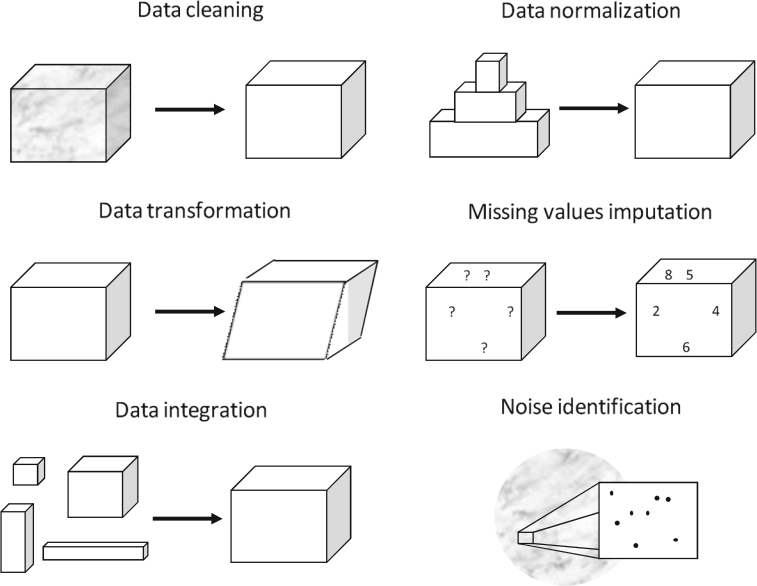
\includegraphics[width=.81\linewidth]{../img/data_preproc.png}}
    \normalcolor\caption{"`Preprocessing Tasks"' aus \cite[Seite 4]{garcia2016big}}
\end{figure}

Die folgenden Unterabschnitte erklären die Vorverarbeitungsschritte für die BfArM-Daten und beziehen sich damit auf die in \ref{abweichungen} genannten Abweichungen. Die Schritte erfolgen in der gelisteten Reihenfolge. Obwohl die Daten nach dem CSV-Parsing schon in einer von der Programmiersprache abhängigen Struktur vorliegen, wird zur Erklärung trotzdem noch die Datei-Struktur verwendet.

\subsection{Datennormalisierung}

\newpara{6-Spalten-Umsteiger}

Sowohl die ICD-10-GM Versionen 2004 und 2.0, als auch die OPS Version 2.1 beinhalteten Umsteiger in folgendem Format:

\codeBoxLD{A00.0;A00.0;A;A;0;UNDEF}{1-202;1-202;A;A;;}

Um diese an das ICD-10-GM Format von 2024 anzupassen, werden die letzten beiden Spalten entfernt. 

\newpara{OPS Umsteiger}

Für OPS Versionen ab 2010 sehen die Umsteiger-Einträge so aus:

\codeBoxL{1-100;N;1-100;N;A;A}

Durch Entfernung der zweiten und vierten Spalte stimmen diese mit den ICD-10-GM Umsteiger Format von 2024 überein. 

\newpara{OPS 6-Spalten-Umsteiger, altes Format}

Die OPS Versionen 2009 bis 2006 hatten ebenfalls sechs Spalten für die Umsteiger, aber in einer anderen Reihenfolge:

\codeBoxL{1-100;1-100;N;N;A;A}

Hier müssen also die dritte und vierte Spalte entfernt werden. 

\newpara{OPS 5-Spalten-Umsteiger}

Die Umsteiger von OPS Version 2005 waren in einem ganz eigenen Format geschrieben:

\codeBoxL{5-062.0;5-062.0;N;A;A\newline
5-062.1;5-062.1;N;A;A\newline
5-062.2;5-062.8;J;E;E\newline
5-062.3;5-062.8;J;B;B}

Hier wird dritte Spalte entfernt und außerdem werden die Sonderformen für automatische Überleitbarkeit von %\texttt{B} und \texttt{E} nach \texttt{A} umbenannt.
$B$ und $E$ nach $A$ umbenannt.  

\newpage

\subsection{Imputation}

Für Umsteiger der OPS Version 2.0 gibt es nur drei Spalten: 

\codeBoxLD{1-208.0;A;1-209.0}{1-208.x;;1-209.4}

Die zweite Spalte zeigt allein die Überleitbarkeit an. Für die Angleichung an das ICD-10-GM Format von 2024 wird also die zweite Spalte entfernt und gedoppelt angehängt. Aus den beiden Beispielzeilen wird damit:

\codeBoxLD{1-208.0;1-209.0;A;A}{1-208.x;1-209.4;;}

\subsection{Datenbereinigung}

\newpara{KOMBI-Kode} Aus OPS Versionen 2.1 und 2.0 wird die erste Zeile der Kode-Datei entfernt, welche den KOMBI-Eintrag enthält. 

\newpara{None statt UNDEF} Für OPS Versionen 2009 bis 2004 wird der Kode-Wert \texttt{None} durch \texttt{UNDEF} ersetzt, sowohl in den Kodes-, als auch in den Umsteiger-Dateien. 

\newpara{Kreuz-Stern-System} Für die ICD-10-GM Versionen 2.0 und 1.3 werden die Zeichen \texttt{+}, \texttt{*} und \texttt{!} aus den Kode-Werten entfernt -- sowohl in der Kodes-, als auch der Umsteiger-Datei.

\newpara{Punkt-Strich-Notation} Für die ICD-10-GM Versionen 2004, 2.0 und 1.3 wird zuerst die Zeichenfolge \texttt{.-} aus den Kode-Werten in beiden Dateitypen entfernt. Danach wird nochmals \texttt{-} entfernt. Die Reihenfolge ist wichtig, weil in Version 2004 zum Beispiel Kodes \texttt{A00.-} und \texttt{G82.1-} vorkommen. 

\subsection{Instanzreduktion}
 
\newpara{Umsteiger}

Für viele Versionen sind über 90\% der Umsteiger-Einträge beidseitig automatische Überleitungen in den gleichen Kode. Diese müssen also gar nicht in eine Applikation aufgenommen werden, unter der Annahme, dass nicht vorhandene Umsteiger damit automatischen Überleitungen entsprechen. Dadurch können alle Umsteiger ausgeschlossen werden, bei denen der neue Kode gleich dem alten Kode ist und die automatische Überleitbarkeit in beide Richtungen gegeben ist. 

\newpage

\newpara{Nicht-endständige Umsteiger}

Die Überleitung von ICD-10-GM Version 2.0 auf 1.3 ist der einzige Fall, in dem die Umsteiger-Datei nicht-endständige Kodes enthält. Durch das Entfernen der Sonderzeichen von Punkt-Strich-Notation und Kreuz-Stern-System gibt es außerdem doppelte Einträge in der ersten Spalte, also bei den Kodes, die sich auf die Vorgänger-Version beziehen.

Folgende Funktion\footnote{Der Pseudocode ist beschrieben in Struktogrammen nach \cite{nassishneid}. Die später vorkommenden Algorithmen zur Umsteiger-Suche enthalten viele Variablenzuweisungen, die abhängig von der Suchrichtung sind und deren parallele Darstellung in Nassi-Shneidermann-Diagrammen übersichtlicher ist. Sie werden also im Sinne der Einheitlichkeit ebenfalls für den Algorithmus in diesem Kapitel verwendet.}
entfernt die überflüssigen Einträge.

Angenommen die Kodes befinden sich in einem Array mit Index von 0 bis (n-1), zum Beispiel für die ersten sechs Zeilen der Umsteiger-Datei aus ICD-10-GM, Überleitung 2.0 nach 1.3: 

\begingroup
\renewcommand{\arraystretch}{1.2}
\setlength{\tabcolsep}{12pt}
\begin{tabular}{cll}
Index & old (Alter Kode) & new (Neuer Kode) \\
\hline
0 & \texttt{A00} & \texttt{A00.0}  \\
1 & \texttt{A00} & \texttt{A00.1} \\
2 & \texttt{A00} & \texttt{A00.9} \\
3 & \texttt{A00.0} & \texttt{A00.0} \\
4 & \texttt{A00.1} & \texttt{A00.1} \\
5 & \texttt{A00.9} & \texttt{A00.9} \\
\end{tabular}
\endgroup

\newpara{removeNonTerminal}

Funktionsparameter:

\begin{itemize}
\item \texttt{\$data} \newline Umsteiger-Einträge
\end{itemize}

Lokale Variablen:

\begin{itemize}
\item \texttt{\$index}
  \newline Der Umsteiger-Eintrag, der aktuell verarbeitet wird.
  \newline Die Funktion läuft vom letztem Eintrag zum ersten.
\item \texttt{\$current}
  \newline Der alte Kode des aktuellen Umsteiger-Eintrags.
  \newline Hierbei bedeutet \$data[ \$index ][ 'old' ] Zugriff auf Zeile mit Index = Wert von \$index und Spalte 'Alter Kode'. Zum Beispiel: data[ 4 ][ 'old' ] = \texttt{A00.1}.
\item \texttt{\$prev}
  \newline Der alte Kode des zuletzt verarbeiteten Umsteiger-Eintrags.
  \newline Die Variable wird auf \$current gesetzt, wenn der Eintrag \emph{nicht} entfernt wird.
\end{itemize}

\newpage

\begin{centernss}
\small
\begin{struktogramm}(120,84)
    \assign[\heightNS]{\$index = count(\$data) - 1}
    \assign[\heightNS]{\$current = \$data[ \$index ][ 'old' ]}
    \while[\heightNS]{WHILE \$index > 0}
    \assign[\heightNS]{\$prev = \$data[ \$index-1 ][ 'old' ]}
    \ifthenelse[24]{2}{2}{IF \$current contains \$prev AND length(\$current) > length(\$prev)}{Y}{N}
        \assign[\heightNS]{remove(\$data[ \$index-1 ])}
    \change
        \assign[\heightNS]{\$current = \$prev}
    \ifend
    \assign[\heightNS]{\$index = \$index - 1}
    \whileend
    \assign[\heightNS]{reindex(\$data)}
\end{struktogramm}
\end{centernss}

\struktkommentar{
 Die IF-Bedingung bezieht sich auf String-basierte Operationen; also contains: "`enthält"' als Sub-String und length: Anzahl der Zeichen im String. \texttt{remove} entfernt eine ganze Zeile, beziehungsweise einen ganzen Umsteiger-Eintrag. 
}

\begin{comment}
\begin{itemize}
\item Die IF-Bedingung bezieht sich auf String-basierte Operationen; also contains: "`enthält"' als Sub-String und length: Anzahl der Zeichen im String.
\item remove: Entfernt eine ganze Zeile. 
\end{itemize}
\end{comment}

Beispiel-Array nach Durchlaufen des Algorithmus:

\begingroup
\renewcommand{\arraystretch}{1.2}
\setlength{\tabcolsep}{12pt}
\begin{tabular}{cll}
Index & old (Alter Kode) & new (Neuer Kode) \\
\hline
0 & \texttt{A00.0} & \texttt{A00.0} \\
1 & \texttt{A00.1} & \texttt{A00.1} \\
2 & \texttt{A00.9} & \texttt{A00.9} \\
\end{tabular}
\endgroup

\newpara{Nicht-endständige Kodes}

Für die meisten Anwendungen sind eigentlich nur die endständigen Kodes relevant. Statt diese bei jeder Operation herauszufiltern, können beim einmaligen Einlesen der Daten auch einfach die nicht-endständigen Kodes ausgeschlossen werden. Zu diesem Zweck kann der oben erklärte Algorithmus ebenfalls eingesetzt werden. 

\subsection{Integration zusätzlicher Informationen}

Das nächst Kapitel erklärt, wie ermittelt wird, ob es zu einem Kode einer bestimmten Version Umsteiger in einer älteren oder neueren Version gibt. Um diese zusätzliche Information speichern zu können, werden die Kodes um eine Spalte erweitert.


\chapter{Umsteiger-Suche} Dieses Kapitel behandelt die versionsübergreifende Suche nach Umsteigern.
%Es geht also zum einen darum zu bestimmen, ob ein bestimmter Kode einer bestimmten Version sich überhaupt verändert hat, sowie zum anderen darum, abhängig von einer Start- und Zielversion zu ermitteln, welche Überleitungen von Kodes möglich sind.
Es geht darum zu bestimmen, ob und wie ein bestimmter Kode in Betrachtung auf alle Versionen des Kodiersystems übergeleitet wurde. 
Die hier aufgeführten Algorithmen sind unabhängig von einer konkreten Implementation verfasst -- als Datenstrukturen werden nur assoziative Arrays, also Maps mit Key$\Rightarrow$Value Paaren, sowie gewöhnliche Arrays mit Index verwendet. 

\section{Allgemeine Funktionen}

Grundlegend ist davon auszugehen, dass Funktionen zum Lesen der Daten vorliegen -- nach erfolgreicher Integration aus dem vorherigen Kapitel. 

\subsection{Daten Lesen}
\label{function-read-data}

Konkret könnten zum Beispiel die Inhalte der Kodes- und Umsteiger-Dateien mit folgenden Parametern ausgelesen werden. 

\newpara{readData}

\begin{itemize}
\item \texttt{\$system} \newline Das Kodiersystem, beispielsweise als Konstanten definiert: \texttt{'icd10gm'} und \texttt{'ops'}. 
\item \texttt{\$version} \newline Die Version, beziehungsweise Jahreszahl.
\item \texttt{\$code} \newline Ein Kode, nach dem gesucht wird. In Bezug auf die Notation von ICD-10-GM und OPS ist es sinnvoll, automatisch an rechter Stelle einen Wildcard zu implizieren -- das heißt einen Platzhalter für beliebige, weitere Zeichen. Dann werden mit einem leeren Wert alle Daten für die anderen Parameter gelesen ohne Einschränkung auf den Kode. 
\item \texttt{\$type} \newline Die Art der Daten, die gelesen werden sollen. Möglich ebenfalls als Konstanten:
  \begin{itemize}
  \item \texttt{'kodes'} \newline Kodes-Daten: Kode und Titel. 
  \item \texttt{'umsteiger'} \newline Umsteiger-Daten: alter Kode und neuer Kode, sowie Information über die automatische Überleitbarkeit in beide Richtungen. Es werden die Umsteiger von der angegebenen auf die nächstältere Version abgefragt. Suche über \texttt{\$code} = neuer Kode. 
  \item \texttt{'umsteiger\_join'} \newline Wie Umsteiger-Daten, aber zusätzlich mit Titel für jeweils den alten und neuen Kode. "`Join"' bezieht sich auf die entsprechende Datenbankoperation.
  \item \texttt{'umsteiger\_join\_alt'} \newline Wie oben, außer dass die Suche über \texttt{\$code} = alter Kode und in die andere Richtung erfolgt. Das heißt es wird die angegebene Version mit der nächstneueren Version verglichen. "`Alt"' für "`alternate direction"'. \\
  \end{itemize}
\end{itemize}

\subsection{Nächste Version}

Außerdem wird eine Funktion benötigt, die ausgehend von System und Version die jeweils nächstältere oder -neuere Version ermittelt. Hierfür kann die in Unterabschnitt \ref{struktdateiversionen} erwähnte strukturierte Datei dienen, welche alle Versionen und Abweichungen definiert.

Wenn keine neuere oder ältere Version existiert, bleibt der Rückgabewert leer.

\newpara{nextNewerVersion / nextOlderVersion}

\begin{figure}[H]
    \centering\large%\sffamily
    \resizebox{.99\linewidth}{!}{% Graphic for TeX using PGF
% Title: /home/simon/jacuke_ma/tex/dia/versions.dia
% Creator: Dia v0.97+git
% CreationDate: Wed Oct 16 06:27:56 2024
% For: simon
% \usepackage{tikz}
% The following commands are not supported in PSTricks at present
% We define them conditionally, so when they are implemented,
% this pgf file will use them.
\ifx\du\undefined
  \newlength{\du}
\fi
\setlength{\du}{15\unitlength}
\begin{tikzpicture}[even odd rule]
\pgftransformxscale{1.000000}
\pgftransformyscale{-1.000000}
\definecolor{dialinecolor}{rgb}{0.000000, 0.000000, 0.000000}
\pgfsetstrokecolor{dialinecolor}
\pgfsetstrokeopacity{1.000000}
\definecolor{diafillcolor}{rgb}{1.000000, 1.000000, 1.000000}
\pgfsetfillcolor{diafillcolor}
\pgfsetfillopacity{1.000000}
\pgfsetlinewidth{0.150000\du}
\pgfsetdash{}{0pt}
\pgfsetbuttcap
{
\definecolor{diafillcolor}{rgb}{0.000000, 0.000000, 0.000000}
\pgfsetfillcolor{diafillcolor}
\pgfsetfillopacity{1.000000}
% was here!!!
\pgfsetarrowsend{stealth}
\definecolor{dialinecolor}{rgb}{0.000000, 0.000000, 0.000000}
\pgfsetstrokecolor{dialinecolor}
\pgfsetstrokeopacity{1.000000}
\draw (-9.000000\du,-15.000000\du)--(-13.000000\du,-15.000000\du);
}
\pgfsetlinewidth{0.150000\du}
\pgfsetdash{}{0pt}
\pgfsetbuttcap
{
\definecolor{diafillcolor}{rgb}{0.000000, 0.000000, 0.000000}
\pgfsetfillcolor{diafillcolor}
\pgfsetfillopacity{1.000000}
% was here!!!
\pgfsetarrowsstart{stealth}
\definecolor{dialinecolor}{rgb}{0.000000, 0.000000, 0.000000}
\pgfsetstrokecolor{dialinecolor}
\pgfsetstrokeopacity{1.000000}
\draw (11.000000\du,-15.000000\du)--(7.000000\du,-15.000000\du);
}
\pgfsetlinewidth{0.000000\du}
\pgfsetdash{}{0pt}
\definecolor{diafillcolor}{rgb}{1.000000, 1.000000, 1.000000}
\pgfsetfillcolor{diafillcolor}
\pgfsetfillopacity{1.000000}
\pgfpathellipse{\pgfpoint{9.000000\du}{-15.000000\du}}{\pgfpoint{1.000000\du}{0\du}}{\pgfpoint{0\du}{1.000000\du}}
\pgfusepath{fill}
\definecolor{dialinecolor}{rgb}{1.000000, 1.000000, 1.000000}
\pgfsetstrokecolor{dialinecolor}
\pgfsetstrokeopacity{1.000000}
\pgfpathellipse{\pgfpoint{9.000000\du}{-15.000000\du}}{\pgfpoint{1.000000\du}{0\du}}{\pgfpoint{0\du}{1.000000\du}}
\pgfusepath{stroke}
\pgfsetlinewidth{0.000000\du}
\pgfsetdash{}{0pt}
\definecolor{diafillcolor}{rgb}{1.000000, 1.000000, 1.000000}
\pgfsetfillcolor{diafillcolor}
\pgfsetfillopacity{1.000000}
\pgfpathellipse{\pgfpoint{-11.000000\du}{-15.000000\du}}{\pgfpoint{1.000000\du}{0\du}}{\pgfpoint{0\du}{1.000000\du}}
\pgfusepath{fill}
\definecolor{dialinecolor}{rgb}{1.000000, 1.000000, 1.000000}
\pgfsetstrokecolor{dialinecolor}
\pgfsetstrokeopacity{1.000000}
\pgfpathellipse{\pgfpoint{-11.000000\du}{-15.000000\du}}{\pgfpoint{1.000000\du}{0\du}}{\pgfpoint{0\du}{1.000000\du}}
\pgfusepath{stroke}
\pgfsetlinewidth{0.100000\du}
\pgfsetdash{}{0pt}
\pgfsetmiterjoin
\pgfsetbuttcap
{\pgfsetcornersarced{\pgfpoint{0.000000\du}{0.000000\du}}\definecolor{dialinecolor}{rgb}{1.000000, 1.000000, 1.000000}
\pgfsetstrokecolor{dialinecolor}
\pgfsetstrokeopacity{1.000000}
\draw (-24.000000\du,-20.000000\du)--(-24.000000\du,-13.000000\du)--(22.000000\du,-13.000000\du)--(22.000000\du,-20.000000\du)--cycle;
}\pgfsetlinewidth{0.100000\du}
\pgfsetdash{}{0pt}
\pgfsetmiterjoin
\pgfsetbuttcap
{\pgfsetcornersarced{\pgfpoint{0.000000\du}{0.000000\du}}\definecolor{diafillcolor}{rgb}{1.000000, 1.000000, 1.000000}
\pgfsetfillcolor{diafillcolor}
\pgfsetfillopacity{1.000000}
\fill (17.000000\du,-16.000000\du)--(17.000000\du,-14.000000\du)--(21.000000\du,-14.000000\du)--(21.000000\du,-16.000000\du)--cycle;
}{\pgfsetcornersarced{\pgfpoint{0.000000\du}{0.000000\du}}\definecolor{dialinecolor}{rgb}{0.000000, 0.000000, 0.000000}
\pgfsetstrokecolor{dialinecolor}
\pgfsetstrokeopacity{1.000000}
\draw (17.000000\du,-16.000000\du)--(17.000000\du,-14.000000\du)--(21.000000\du,-14.000000\du)--(21.000000\du,-16.000000\du)--cycle;
}\pgfsetlinewidth{0.100000\du}
\pgfsetdash{}{0pt}
\pgfsetmiterjoin
\pgfsetbuttcap
{\pgfsetcornersarced{\pgfpoint{0.000000\du}{0.000000\du}}\definecolor{diafillcolor}{rgb}{1.000000, 1.000000, 1.000000}
\pgfsetfillcolor{diafillcolor}
\pgfsetfillopacity{1.000000}
\fill (11.000000\du,-16.000000\du)--(11.000000\du,-14.000000\du)--(15.000000\du,-14.000000\du)--(15.000000\du,-16.000000\du)--cycle;
}{\pgfsetcornersarced{\pgfpoint{0.000000\du}{0.000000\du}}\definecolor{dialinecolor}{rgb}{0.000000, 0.000000, 0.000000}
\pgfsetstrokecolor{dialinecolor}
\pgfsetstrokeopacity{1.000000}
\draw (11.000000\du,-16.000000\du)--(11.000000\du,-14.000000\du)--(15.000000\du,-14.000000\du)--(15.000000\du,-16.000000\du)--cycle;
}\pgfsetlinewidth{0.100000\du}
\pgfsetdash{}{0pt}
\pgfsetmiterjoin
\pgfsetbuttcap
{\pgfsetcornersarced{\pgfpoint{0.000000\du}{0.000000\du}}\definecolor{diafillcolor}{rgb}{1.000000, 1.000000, 1.000000}
\pgfsetfillcolor{diafillcolor}
\pgfsetfillopacity{1.000000}
\fill (3.000000\du,-16.000000\du)--(3.000000\du,-14.000000\du)--(7.000000\du,-14.000000\du)--(7.000000\du,-16.000000\du)--cycle;
}{\pgfsetcornersarced{\pgfpoint{0.000000\du}{0.000000\du}}\definecolor{dialinecolor}{rgb}{0.000000, 0.000000, 0.000000}
\pgfsetstrokecolor{dialinecolor}
\pgfsetstrokeopacity{1.000000}
\draw (3.000000\du,-16.000000\du)--(3.000000\du,-14.000000\du)--(7.000000\du,-14.000000\du)--(7.000000\du,-16.000000\du)--cycle;
}\pgfsetlinewidth{0.100000\du}
\pgfsetdash{}{0pt}
\pgfsetmiterjoin
\pgfsetbuttcap
{\pgfsetcornersarced{\pgfpoint{0.000000\du}{0.000000\du}}\definecolor{diafillcolor}{rgb}{1.000000, 1.000000, 1.000000}
\pgfsetfillcolor{diafillcolor}
\pgfsetfillopacity{1.000000}
\fill (-23.000000\du,-16.000000\du)--(-23.000000\du,-14.000000\du)--(-19.000000\du,-14.000000\du)--(-19.000000\du,-16.000000\du)--cycle;
}{\pgfsetcornersarced{\pgfpoint{0.000000\du}{0.000000\du}}\definecolor{dialinecolor}{rgb}{0.000000, 0.000000, 0.000000}
\pgfsetstrokecolor{dialinecolor}
\pgfsetstrokeopacity{1.000000}
\draw (-23.000000\du,-16.000000\du)--(-23.000000\du,-14.000000\du)--(-19.000000\du,-14.000000\du)--(-19.000000\du,-16.000000\du)--cycle;
}\pgfsetlinewidth{0.100000\du}
\pgfsetdash{}{0pt}
\pgfsetmiterjoin
\pgfsetbuttcap
{\pgfsetcornersarced{\pgfpoint{0.000000\du}{0.000000\du}}\definecolor{diafillcolor}{rgb}{1.000000, 1.000000, 1.000000}
\pgfsetfillcolor{diafillcolor}
\pgfsetfillopacity{1.000000}
\fill (-17.000000\du,-16.000000\du)--(-17.000000\du,-14.000000\du)--(-13.000000\du,-14.000000\du)--(-13.000000\du,-16.000000\du)--cycle;
}{\pgfsetcornersarced{\pgfpoint{0.000000\du}{0.000000\du}}\definecolor{dialinecolor}{rgb}{0.000000, 0.000000, 0.000000}
\pgfsetstrokecolor{dialinecolor}
\pgfsetstrokeopacity{1.000000}
\draw (-17.000000\du,-16.000000\du)--(-17.000000\du,-14.000000\du)--(-13.000000\du,-14.000000\du)--(-13.000000\du,-16.000000\du)--cycle;
}\pgfsetlinewidth{0.100000\du}
\pgfsetdash{}{0pt}
\pgfsetmiterjoin
\pgfsetbuttcap
{\pgfsetcornersarced{\pgfpoint{0.000000\du}{0.000000\du}}\definecolor{diafillcolor}{rgb}{1.000000, 1.000000, 1.000000}
\pgfsetfillcolor{diafillcolor}
\pgfsetfillopacity{1.000000}
\fill (-9.000000\du,-16.000000\du)--(-9.000000\du,-14.000000\du)--(-5.000000\du,-14.000000\du)--(-5.000000\du,-16.000000\du)--cycle;
}{\pgfsetcornersarced{\pgfpoint{0.000000\du}{0.000000\du}}\definecolor{dialinecolor}{rgb}{0.000000, 0.000000, 0.000000}
\pgfsetstrokecolor{dialinecolor}
\pgfsetstrokeopacity{1.000000}
\draw (-9.000000\du,-16.000000\du)--(-9.000000\du,-14.000000\du)--(-5.000000\du,-14.000000\du)--(-5.000000\du,-16.000000\du)--cycle;
}% setfont left to latex
\definecolor{dialinecolor}{rgb}{0.000000, 0.000000, 0.000000}
\pgfsetstrokecolor{dialinecolor}
\pgfsetstrokeopacity{1.000000}
\definecolor{diafillcolor}{rgb}{0.000000, 0.000000, 0.000000}
\pgfsetfillcolor{diafillcolor}
\pgfsetfillopacity{1.000000}
\node[anchor=base,inner sep=0pt, outer sep=0pt,color=dialinecolor] at (-15.000000\du,-14.687351\du){2024};
% setfont left to latex
\definecolor{dialinecolor}{rgb}{0.000000, 0.000000, 0.000000}
\pgfsetstrokecolor{dialinecolor}
\pgfsetstrokeopacity{1.000000}
\definecolor{diafillcolor}{rgb}{0.000000, 0.000000, 0.000000}
\pgfsetfillcolor{diafillcolor}
\pgfsetfillopacity{1.000000}
\node[anchor=base,inner sep=0pt, outer sep=0pt,color=dialinecolor] at (13.000000\du,-14.687351\du){1.3};
% setfont left to latex
\definecolor{dialinecolor}{rgb}{0.000000, 0.000000, 0.000000}
\pgfsetstrokecolor{dialinecolor}
\pgfsetstrokeopacity{1.000000}
\definecolor{diafillcolor}{rgb}{0.000000, 0.000000, 0.000000}
\pgfsetfillcolor{diafillcolor}
\pgfsetfillopacity{1.000000}
\node[anchor=base,inner sep=0pt, outer sep=0pt,color=dialinecolor] at (-11.000000\du,-14.687351\du){...};
% setfont left to latex
\definecolor{dialinecolor}{rgb}{0.000000, 0.000000, 0.000000}
\pgfsetstrokecolor{dialinecolor}
\pgfsetstrokeopacity{1.000000}
\definecolor{diafillcolor}{rgb}{0.000000, 0.000000, 0.000000}
\pgfsetfillcolor{diafillcolor}
\pgfsetfillopacity{1.000000}
\node[anchor=base,inner sep=0pt, outer sep=0pt,color=dialinecolor] at (9.000000\du,-14.687351\du){...};
% setfont left to latex
\definecolor{dialinecolor}{rgb}{0.000000, 0.000000, 0.000000}
\pgfsetstrokecolor{dialinecolor}
\pgfsetstrokeopacity{1.000000}
\definecolor{diafillcolor}{rgb}{0.000000, 0.000000, 0.000000}
\pgfsetfillcolor{diafillcolor}
\pgfsetfillopacity{1.000000}
\node[anchor=base,inner sep=0pt, outer sep=0pt,color=dialinecolor] at (-7.000000\du,-14.687351\du){2014};
% setfont left to latex
\definecolor{dialinecolor}{rgb}{0.000000, 0.000000, 0.000000}
\pgfsetstrokecolor{dialinecolor}
\pgfsetstrokeopacity{1.000000}
\definecolor{diafillcolor}{rgb}{0.000000, 0.000000, 0.000000}
\pgfsetfillcolor{diafillcolor}
\pgfsetfillopacity{1.000000}
\node[anchor=base,inner sep=0pt, outer sep=0pt,color=dialinecolor] at (5.000000\du,-14.687351\du){2012};
\pgfsetlinewidth{0.150000\du}
\pgfsetdash{}{0pt}
\pgfsetbuttcap
{
\definecolor{diafillcolor}{rgb}{0.000000, 0.000000, 0.000000}
\pgfsetfillcolor{diafillcolor}
\pgfsetfillopacity{1.000000}
% was here!!!
\pgfsetarrowsend{stealth}
\definecolor{dialinecolor}{rgb}{0.000000, 0.000000, 0.000000}
\pgfsetstrokecolor{dialinecolor}
\pgfsetstrokeopacity{1.000000}
\pgfpathmoveto{\pgfpoint{-0.999992\du}{-15.999980\du}}
\pgfpatharc{338}{203}{3.250000\du and 3.250000\du}
\pgfusepath{stroke}
}
\definecolor{diafillcolor}{rgb}{1.000000, 1.000000, 1.000000}
\pgfsetfillcolor{diafillcolor}
\pgfsetfillopacity{1.000000}
\fill (-11.217500\du,-19.525637\du)--(-3.000000\du,-19.525637\du)--(-3.000000\du,-18.474363\du)--(-11.217500\du,-18.474363\du)--cycle;
% setfont left to latex
\definecolor{dialinecolor}{rgb}{0.000000, 0.000000, 0.000000}
\pgfsetstrokecolor{dialinecolor}
\pgfsetstrokeopacity{1.000000}
\definecolor{diafillcolor}{rgb}{0.000000, 0.000000, 0.000000}
\pgfsetfillcolor{diafillcolor}
\pgfsetfillopacity{1.000000}
\node[anchor=base east,inner sep=0pt, outer sep=0pt,color=dialinecolor] at (-3.000000\du,-18.687351\du){nextNewerVersion};
% setfont left to latex
\definecolor{dialinecolor}{rgb}{0.000000, 0.000000, 0.000000}
\pgfsetstrokecolor{dialinecolor}
\pgfsetstrokeopacity{1.000000}
\definecolor{diafillcolor}{rgb}{0.000000, 0.000000, 0.000000}
\pgfsetfillcolor{diafillcolor}
\pgfsetfillopacity{1.000000}
\node[anchor=base west,inner sep=0pt,outer sep=0pt,color=dialinecolor] at (1.000000\du,-18.687351\du){nextOlderVersion};
\pgfsetlinewidth{0.100000\du}
\pgfsetdash{}{0pt}
\pgfsetmiterjoin
\pgfsetbuttcap
{\pgfsetcornersarced{\pgfpoint{0.000000\du}{0.000000\du}}\definecolor{diafillcolor}{rgb}{1.000000, 1.000000, 1.000000}
\pgfsetfillcolor{diafillcolor}
\pgfsetfillopacity{1.000000}
\fill (-3.000000\du,-16.000000\du)--(-3.000000\du,-14.000000\du)--(1.000000\du,-14.000000\du)--(1.000000\du,-16.000000\du)--cycle;
}{\pgfsetcornersarced{\pgfpoint{0.000000\du}{0.000000\du}}\definecolor{dialinecolor}{rgb}{0.000000, 0.000000, 0.000000}
\pgfsetstrokecolor{dialinecolor}
\pgfsetstrokeopacity{1.000000}
\draw (-3.000000\du,-16.000000\du)--(-3.000000\du,-14.000000\du)--(1.000000\du,-14.000000\du)--(1.000000\du,-16.000000\du)--cycle;
}% setfont left to latex
\definecolor{dialinecolor}{rgb}{0.000000, 0.000000, 0.000000}
\pgfsetstrokecolor{dialinecolor}
\pgfsetstrokeopacity{1.000000}
\definecolor{diafillcolor}{rgb}{0.000000, 0.000000, 0.000000}
\pgfsetfillcolor{diafillcolor}
\pgfsetfillopacity{1.000000}
\node[anchor=base,inner sep=0pt, outer sep=0pt,color=dialinecolor] at (-1.000000\du,-14.687351\du){2013};
\pgfsetlinewidth{0.150000\du}
\pgfsetdash{}{0pt}
\pgfsetbuttcap
{
\definecolor{diafillcolor}{rgb}{0.000000, 0.000000, 0.000000}
\pgfsetfillcolor{diafillcolor}
\pgfsetfillopacity{1.000000}
% was here!!!
\pgfsetarrowsend{stealth}
\definecolor{dialinecolor}{rgb}{0.000000, 0.000000, 0.000000}
\pgfsetstrokecolor{dialinecolor}
\pgfsetstrokeopacity{1.000000}
\draw (-17.000000\du,-15.000000\du)--(-19.000000\du,-15.000000\du);
}
\pgfsetlinewidth{0.150000\du}
\pgfsetdash{}{0pt}
\pgfsetbuttcap
{
\definecolor{diafillcolor}{rgb}{0.000000, 0.000000, 0.000000}
\pgfsetfillcolor{diafillcolor}
\pgfsetfillopacity{1.000000}
% was here!!!
\pgfsetarrowsstart{stealth}
\definecolor{dialinecolor}{rgb}{0.000000, 0.000000, 0.000000}
\pgfsetstrokecolor{dialinecolor}
\pgfsetstrokeopacity{1.000000}
\draw (17.000000\du,-15.000000\du)--(15.000000\du,-15.000000\du);
}
\pgfsetlinewidth{0.150000\du}
\pgfsetdash{}{0pt}
\pgfsetbuttcap
{
\definecolor{diafillcolor}{rgb}{0.000000, 0.000000, 0.000000}
\pgfsetfillcolor{diafillcolor}
\pgfsetfillopacity{1.000000}
% was here!!!
\pgfsetarrowsstart{stealth}
\definecolor{dialinecolor}{rgb}{0.000000, 0.000000, 0.000000}
\pgfsetstrokecolor{dialinecolor}
\pgfsetstrokeopacity{1.000000}
\pgfpathmoveto{\pgfpoint{5.000008\du}{-15.999980\du}}
\pgfpatharc{338}{203}{3.250000\du and 3.250000\du}
\pgfusepath{stroke}
}
\end{tikzpicture}
}
    \normalsize\vspace{-1em}\caption{Ermitteln der nächstliegenden Versionen am Beispiel von ICD-10-GM.}
\end{figure}

\subsection{Beispieldaten mit graphischer Darstellung}

Um beispielsweise die Kodes M21.4 und M21.6 aus der ICD-10-GM Version 2016 mit der Funktion readData abzufragen, sehen die Aufrufe so aus:

\texttt{readData ('icd10gm', '2014', 'M21.4', 'kodes')} \newline
\texttt{readData ('icd10gm', '2014', 'M21.6', 'kodes')}

\newpage

Die Ergebnisse in Tabellenform:

%\begingroup
\begin{centernss}
\renewcommand{\arraystretch}{1.2}
\setlength{\tabcolsep}{12pt}
\begin{tabular}{ll}
code (Kode) & name (Titel) \\
\hline
M21.4 & Plattfuß [Pes planus] (erworben) \\
M21.6 & Sonstige erworbene Deformitäten des Knöchels und des Fußes \\
\end{tabular}
\end{centernss}
%\endgroup

%\ \newline

Für das restliche Kapitel wird angenommen, dass die Ergebnisse der readData-Funktion in einer zweidimensionalen Datenstruktur gespeichert werden, die einer Tabelle ähnelt -- das heißt eine Array-Liste mit einem Eintrag pro Zeile beginnend mit Index = 0, sowie einem assoziativen Array (Map oder alternativ eine Klassenstruktur) mit Key = Spaltenüberschrift. Der Zugriff auf den Titel "`Plattfuß"' in deren oberen Tabelle erfolgt dann über \texttt{\$data[ 0 ][ 'name' ]}.

(Mit dem \$-Zeichen werden Variablennamen hervorgehoben.) \\

Analog zu den Kodes können die Umsteiger wie folgt abgefragt werden: \newline
\texttt{lies\_daten ('icd10gm', '2014', 'M21.4', 'umsteiger')} \newline
\texttt{lies\_daten ('icd10gm', '2014', 'M21.6', 'umsteiger')} \\

Resultierend in:

%\begingroup
\begin{centernss}
\renewcommand{\arraystretch}{1.2}
\begin{tabular}{p{136pt}p{136pt}lr}
new (Kode Version 2014) & old (Kode Version 2013) & \multicolumn{2}{c}{$\leftarrow$Auto$\rightarrow$} \\
\hline
M21.4 & M21.4 & A & A \\
M21.6 & M21.6 & A & A \\
\end{tabular}
\end{centernss}
%\endgroup

``Auto'' steht für die automatische Überleitbarkeit in die jeweilige Richtung, das heißt 2014$\leftarrow$2013 und 2014$\rightarrow$2013. \\

Von Version 2014 auf 2013 ändern sich die angegebenen ICD-10-GM Kodes nicht. Sie sind auch in beide Richtungen automatisch überleitbar. Wie bereits in der Datenintegration erwähnt, müssen diese Einträge eigentlich gar nicht aufgenommen werden. Sie sind hier nur zur Vereinfachung aufgelistet, weil die Einträge auch so in den BfArM-Dateien enthalten sind. Bei der versionsübergreifenden Suche nach Umsteigern sind allerdings nur die Veränderungen relevant. Anstatt alle nicht relevanten Umsteiger-Einträge abzuspeichern und bei jeder Abfrage auszuschließen, kann alternativ auch angenommen werden, dass bei Nichtvorhandensein eines Umsteigers zwischen zwei Versionen dieser Kode einfach gleich bleibt. Die Suche nach Umsteigern geht immer von einem vorhanden Kode aus.

\emph{Wichtig:} Für den Rest des Kapitels bedeutet Umsteiger, dass bei der Überleitung eines Kodes von der alten auf die neue Version wirklich eine Veränderung vorliegt. 

\newpage

M21.4 hat also keine Umsteiger. M21.6 hat folgende: \newline

\begin{centernss}
\renewcommand{\arraystretch}{1.2}
\begin{tabular}{p{136pt}p{136pt}lr}
new (Kode Version 2015) & old (Kode Version 2014) & \multicolumn{2}{c}{$\leftarrow$Auto$\rightarrow$} \\
\hline
%M21.4 & M21.4 & A & A \\
%\cline{1-1}%\hline%\hdashline[0.5pt/5pt]
M21.60 & M21.6 & & A \\
M21.61 & M21.6 & & A \\
M21.62 & M21.6 & & A \\
M21.63 & M21.6 & & A \\
M21.68 & M21.6 & & A \\
\end{tabular}
\end{centernss}

\begin{centernss}
\renewcommand{\arraystretch}{1.2}
\begin{tabular}{p{136pt}p{136pt}lr}
new (Kode Version 2013) & old (Kode Version 2012) & \multicolumn{2}{c}{$\leftarrow$Auto$\rightarrow$} \\
\hline
%M21.4 & M21.4 & A & A \\
%\cline{1-1}%\hline%\hdashline[0.5pt/5pt]
M21.6 & M21.60 & A &  \\
M21.6 & M21.67 & A &  \\
M21.6 & M21.87 & A & A \\
\end{tabular}
\end{centernss}

\begin{comment}
\begin{centernss}
\renewcommand{\arraystretch}{1.2}
\begin{tabular}{p{136pt}p{136pt}lr}
new (Kode Version 2.0) & old (Kode Version 1.3) & \multicolumn{2}{c}{$\leftarrow$Auto$\rightarrow$} \\
\hline
M21.4 & M21.4 & A & A \\
%\cline{1-1}%\hline%\hdashline[0.5pt/5pt]
M21.60 & M21.6 &  & A \\
M21.67 & M21.6 &  & A \\
%\cline{1-1}%\hline%\hdashline[0.5pt/5pt]
M21.80 & M21.8 &  & A \\
M21.81 & M21.8 &  & A \\
M21.82 & M21.8 &  & A \\
M21.83 & M21.8 &  & A \\
M21.84 & M21.8 &  & A \\
M21.85 & M21.8 &  & A \\
M21.86 & M21.8 &  & A \\
M21.87 & M21.8 &  & A \\
M21.88 & M21.8 &  & A \\
M21.89 & M21.8 & A & A \\
\end{tabular}
\end{centernss}
\end{comment}

\ \newline Die Suche wird ab Version 2012 mit M21.60, M21.67 und M21.87 fortgesetzt: 

\begin{centernss}
\renewcommand{\arraystretch}{1.2}
\begin{tabular}{p{136pt}p{136pt}lr}
new (Kode Version 2.0) & old (Kode Version 1.3) & \multicolumn{2}{c}{$\leftarrow$Auto$\rightarrow$} \\
\hline
%M21.4 & M21.4 & A & A \\
%\cline{1-1}%\hline%\hdashline[0.5pt/5pt]
M21.60 & M21.6 &  & A \\
M21.67 & M21.6 &  & A \\
%\cline{1-1}%\hline%\hdashline[0.5pt/5pt]
M21.80 & M21.8 &  & A \\
M21.81 & M21.8 &  & A \\
M21.82 & M21.8 &  & A \\
M21.83 & M21.8 &  & A \\
M21.84 & M21.8 &  & A \\
M21.85 & M21.8 &  & A \\
M21.86 & M21.8 &  & A \\
M21.87 & M21.8 &  & A \\
M21.88 & M21.8 &  & A \\
M21.89 & M21.8 & A & A \\
\end{tabular}
\end{centernss}

\ \\

%Anmerkung: Von Kode M21.8, Version 1.3. ausgehend gibt es noch wesentlich mehr Umsteiger, aber diese werden hier nicht gelistet, weil sie sind von M21.6, Version 2014 aus nicht erreichbar sind. 

Anmerkung: Die Umsteiger für Kode M21.8, Version 1.3. sind nur zur Vollständigkeit gelistet. Von M21.6, Version 2014 ausgehend ist nur M21.87, Version 2.0 erreichbar.

\begin{comment}

\begin{minipage}[t]{.5\textwidth}\vspace{0pt}
%
\begingroup
\begin{tabular}{p{58pt}p{58pt}lr}
new (2015) & old (2014) & \multicolumn{2}{c}{$\leftarrow$Auto$\rightarrow$} \\
\hline
M21.4 & M21.4 & A & A \\
\cline{1-1}%\hline%\hdashline[0.5pt/5pt]
M21.60 & M21.6 & & A \\
M21.61 & M21.6 & & A \\
M21.62 & M21.6 & & A \\
M21.63 & M21.6 & & A \\
M21.68 & M21.6 & & A \\
\end{tabular}
%

\ \\

%\ \\

%
\begin{tabular}{p{58pt}p{58pt}lr}
new (2013) & old (2012) & \multicolumn{2}{c}{$\leftarrow$Auto$\rightarrow$} \\
\hline
M21.4 & M21.4 & A & A \\
\cline{1-1}%\hline%\hdashline[0.5pt/5pt]
M21.6 & M21.60 & A &  \\
M21.6 & M21.67 & A &  \\
M21.6 & M21.87 & A & A \\
\end{tabular}
\endgroup
%
\end{minipage}
\begin{minipage}[t]{.5\textwidth}%\vspace{0pt}
%
\begingroup
\renewcommand{\arraystretch}{1.2}
\begin{tabular}[t]{p{58pt}p{58pt}lr}
new (2.0) & old (1.3) & \multicolumn{2}{c}{$\leftarrow$Auto$\rightarrow$} \\
\hline
M21.4 & M21.4 & A & A \\
\cline{1-1}%\hline%\hdashline[0.5pt/5pt]
M21.60 & M21.6 &  & A \\
M21.67 & M21.6 &  & A \\
\cline{1-1}%\hline%\hdashline[0.5pt/5pt]
M21.80 & M21.8 &  & A \\
M21.81 & M21.8 &  & A \\
M21.82 & M21.8 &  & A \\
M21.83 & M21.8 &  & A \\
M21.84 & M21.8 &  & A \\
M21.85 & M21.8 &  & A \\
M21.86 & M21.8 &  & A \\
M21.87 & M21.8 &  & A \\
M21.88 & M21.8 &  & A \\
M21.89 & M21.8 & A & A \\
\end{tabular}
\endgroup
%
\end{minipage}
\end{comment}




\begin{comment}

2.0

M21.6;M21.60;;A
M21.6;M21.67;;A

M21.8;M21.80;;A
M21.8;M21.81;;A
M21.8;M21.82;;A
M21.8;M21.83;;A
M21.8;M21.84;;A
M21.8;M21.85;;A
M21.8;M21.86;;A
M21.8;M21.87;;A
M21.8;M21.88;;A
M21.8;M21.89;A;A

\end{comment}

Die Ergebnisse können als Graph dargestellt werden; siehe nächste Seite. Die Versionen sind horizontal angeordnet und die Kodes pro Version vertikal darunter als Knoten. Ausgangspunkt sind wie erwähnt die Kodes M21.4 und M21.6 der Version 2014. Die Knoten der anderen Versionen entsprechen den Kodes, die über Umsteiger erreichbar sind. Die Pfeilspitzen geben die Richtung der automatischen Überleitbarkeit an. 

\begin{figure}[H]
    \centering\Large%\sffamily
    \resizebox{.99\linewidth}{!}{% Graphic for TeX using PGF
% Title: /home/simon/jacuke_ma/tex/dia/nodes.dia
% Creator: Dia v0.97+git
% CreationDate: Fri Sep 20 16:05:51 2024
% For: simon
% \usepackage{tikz}
% The following commands are not supported in PSTricks at present
% We define them conditionally, so when they are implemented,
% this pgf file will use them.
\ifx\du\undefined
  \newlength{\du}
\fi
\setlength{\du}{15\unitlength}
\begin{tikzpicture}[even odd rule]
\pgftransformxscale{1.000000}
\pgftransformyscale{-1.000000}
\definecolor{dialinecolor}{rgb}{0.000000, 0.000000, 0.000000}
\pgfsetstrokecolor{dialinecolor}
\pgfsetstrokeopacity{1.000000}
\definecolor{diafillcolor}{rgb}{1.000000, 1.000000, 1.000000}
\pgfsetfillcolor{diafillcolor}
\pgfsetfillopacity{1.000000}
\pgfsetlinewidth{0.100000\du}
\pgfsetdash{}{0pt}
\pgfsetmiterjoin
\pgfsetbuttcap
{\pgfsetcornersarced{\pgfpoint{0.000000\du}{0.000000\du}}\definecolor{diafillcolor}{rgb}{1.000000, 1.000000, 1.000000}
\pgfsetfillcolor{diafillcolor}
\pgfsetfillopacity{0.117647}
\fill (-24.000000\du,-13.000000\du)--(-24.000000\du,28.000000\du)--(22.000000\du,28.000000\du)--(22.000000\du,-13.000000\du)--cycle;
}{\pgfsetcornersarced{\pgfpoint{0.000000\du}{0.000000\du}}\definecolor{dialinecolor}{rgb}{1.000000, 1.000000, 1.000000}
\pgfsetstrokecolor{dialinecolor}
\pgfsetstrokeopacity{1.000000}
\draw (-24.000000\du,-13.000000\du)--(-24.000000\du,28.000000\du)--(22.000000\du,28.000000\du)--(22.000000\du,-13.000000\du)--cycle;
}\pgfsetlinewidth{0.100000\du}
\pgfsetdash{{0.500000\du}{0.500000\du}}{0\du}
\pgfsetbuttcap
{
\definecolor{diafillcolor}{rgb}{0.411765, 0.411765, 0.411765}
\pgfsetfillcolor{diafillcolor}
\pgfsetfillopacity{1.000000}
% was here!!!
\definecolor{dialinecolor}{rgb}{0.411765, 0.411765, 0.411765}
\pgfsetstrokecolor{dialinecolor}
\pgfsetstrokeopacity{1.000000}
\draw (19.000000\du,-10.000000\du)--(19.000000\du,28.000000\du);
}
\pgfsetlinewidth{0.100000\du}
\pgfsetdash{{0.500000\du}{0.500000\du}}{0\du}
\pgfsetbuttcap
{
\definecolor{diafillcolor}{rgb}{0.411765, 0.411765, 0.411765}
\pgfsetfillcolor{diafillcolor}
\pgfsetfillopacity{1.000000}
% was here!!!
\definecolor{dialinecolor}{rgb}{0.411765, 0.411765, 0.411765}
\pgfsetstrokecolor{dialinecolor}
\pgfsetstrokeopacity{1.000000}
\draw (13.000000\du,-10.000000\du)--(13.000000\du,28.000000\du);
}
\pgfsetlinewidth{0.100000\du}
\pgfsetdash{}{0pt}
\pgfsetmiterjoin
\pgfsetbuttcap
{\pgfsetcornersarced{\pgfpoint{0.000000\du}{0.000000\du}}\definecolor{diafillcolor}{rgb}{1.000000, 1.000000, 1.000000}
\pgfsetfillcolor{diafillcolor}
\pgfsetfillopacity{1.000000}
\fill (11.000000\du,-12.000000\du)--(11.000000\du,-10.000000\du)--(15.000000\du,-10.000000\du)--(15.000000\du,-12.000000\du)--cycle;
}{\pgfsetcornersarced{\pgfpoint{0.000000\du}{0.000000\du}}\definecolor{dialinecolor}{rgb}{0.411765, 0.411765, 0.411765}
\pgfsetstrokecolor{dialinecolor}
\pgfsetstrokeopacity{1.000000}
\draw (11.000000\du,-12.000000\du)--(11.000000\du,-10.000000\du)--(15.000000\du,-10.000000\du)--(15.000000\du,-12.000000\du)--cycle;
}% setfont left to latex
\definecolor{dialinecolor}{rgb}{0.411765, 0.411765, 0.411765}
\pgfsetstrokecolor{dialinecolor}
\pgfsetstrokeopacity{1.000000}
\definecolor{diafillcolor}{rgb}{0.411765, 0.411765, 0.411765}
\pgfsetfillcolor{diafillcolor}
\pgfsetfillopacity{1.000000}
\node[anchor=base,inner sep=0pt, outer sep=0pt,color=dialinecolor] at (13.000000\du,-10.687351\du){2.0};
\pgfsetlinewidth{0.100000\du}
\pgfsetdash{{0.500000\du}{0.500000\du}}{0\du}
\pgfsetbuttcap
{
\definecolor{diafillcolor}{rgb}{0.411765, 0.411765, 0.411765}
\pgfsetfillcolor{diafillcolor}
\pgfsetfillopacity{1.000000}
% was here!!!
\definecolor{dialinecolor}{rgb}{0.411765, 0.411765, 0.411765}
\pgfsetstrokecolor{dialinecolor}
\pgfsetstrokeopacity{1.000000}
\draw (5.000000\du,-10.000000\du)--(5.000000\du,28.000000\du);
}
\pgfsetlinewidth{0.100000\du}
\pgfsetdash{}{0pt}
\pgfsetmiterjoin
\pgfsetbuttcap
{\pgfsetcornersarced{\pgfpoint{0.000000\du}{0.000000\du}}\definecolor{diafillcolor}{rgb}{1.000000, 1.000000, 1.000000}
\pgfsetfillcolor{diafillcolor}
\pgfsetfillopacity{1.000000}
\fill (3.000000\du,-12.000000\du)--(3.000000\du,-10.000000\du)--(7.000000\du,-10.000000\du)--(7.000000\du,-12.000000\du)--cycle;
}{\pgfsetcornersarced{\pgfpoint{0.000000\du}{0.000000\du}}\definecolor{dialinecolor}{rgb}{0.411765, 0.411765, 0.411765}
\pgfsetstrokecolor{dialinecolor}
\pgfsetstrokeopacity{1.000000}
\draw (3.000000\du,-12.000000\du)--(3.000000\du,-10.000000\du)--(7.000000\du,-10.000000\du)--(7.000000\du,-12.000000\du)--cycle;
}% setfont left to latex
\definecolor{dialinecolor}{rgb}{0.411765, 0.411765, 0.411765}
\pgfsetstrokecolor{dialinecolor}
\pgfsetstrokeopacity{1.000000}
\definecolor{diafillcolor}{rgb}{0.411765, 0.411765, 0.411765}
\pgfsetfillcolor{diafillcolor}
\pgfsetfillopacity{1.000000}
\node[anchor=base,inner sep=0pt, outer sep=0pt,color=dialinecolor] at (5.000000\du,-10.687351\du){2012};
\pgfsetlinewidth{0.100000\du}
\pgfsetdash{{0.500000\du}{0.500000\du}}{0\du}
\pgfsetbuttcap
{
\definecolor{diafillcolor}{rgb}{0.411765, 0.411765, 0.411765}
\pgfsetfillcolor{diafillcolor}
\pgfsetfillopacity{1.000000}
% was here!!!
\definecolor{dialinecolor}{rgb}{0.411765, 0.411765, 0.411765}
\pgfsetstrokecolor{dialinecolor}
\pgfsetstrokeopacity{1.000000}
\draw (-1.000000\du,-10.000000\du)--(-1.000000\du,28.000000\du);
}
\pgfsetlinewidth{0.100000\du}
\pgfsetdash{}{0pt}
\pgfsetmiterjoin
\pgfsetbuttcap
{\pgfsetcornersarced{\pgfpoint{0.000000\du}{0.000000\du}}\definecolor{diafillcolor}{rgb}{1.000000, 1.000000, 1.000000}
\pgfsetfillcolor{diafillcolor}
\pgfsetfillopacity{1.000000}
\fill (-3.000000\du,-12.000000\du)--(-3.000000\du,-10.000000\du)--(1.000000\du,-10.000000\du)--(1.000000\du,-12.000000\du)--cycle;
}{\pgfsetcornersarced{\pgfpoint{0.000000\du}{0.000000\du}}\definecolor{dialinecolor}{rgb}{0.411765, 0.411765, 0.411765}
\pgfsetstrokecolor{dialinecolor}
\pgfsetstrokeopacity{1.000000}
\draw (-3.000000\du,-12.000000\du)--(-3.000000\du,-10.000000\du)--(1.000000\du,-10.000000\du)--(1.000000\du,-12.000000\du)--cycle;
}% setfont left to latex
\definecolor{dialinecolor}{rgb}{0.411765, 0.411765, 0.411765}
\pgfsetstrokecolor{dialinecolor}
\pgfsetstrokeopacity{1.000000}
\definecolor{diafillcolor}{rgb}{0.411765, 0.411765, 0.411765}
\pgfsetfillcolor{diafillcolor}
\pgfsetfillopacity{1.000000}
\node[anchor=base,inner sep=0pt, outer sep=0pt,color=dialinecolor] at (-1.000000\du,-10.687351\du){2013};
\pgfsetlinewidth{0.100000\du}
\pgfsetdash{{0.500000\du}{0.500000\du}}{0\du}
\pgfsetbuttcap
{
\definecolor{diafillcolor}{rgb}{0.411765, 0.411765, 0.411765}
\pgfsetfillcolor{diafillcolor}
\pgfsetfillopacity{1.000000}
% was here!!!
\definecolor{dialinecolor}{rgb}{0.411765, 0.411765, 0.411765}
\pgfsetstrokecolor{dialinecolor}
\pgfsetstrokeopacity{1.000000}
\draw (-7.000000\du,-10.000000\du)--(-7.000000\du,28.000000\du);
}
\pgfsetlinewidth{0.100000\du}
\pgfsetdash{}{0pt}
\pgfsetmiterjoin
\pgfsetbuttcap
{\pgfsetcornersarced{\pgfpoint{0.000000\du}{0.000000\du}}\definecolor{diafillcolor}{rgb}{1.000000, 1.000000, 1.000000}
\pgfsetfillcolor{diafillcolor}
\pgfsetfillopacity{1.000000}
\fill (-9.000000\du,-12.000000\du)--(-9.000000\du,-10.000000\du)--(-5.000000\du,-10.000000\du)--(-5.000000\du,-12.000000\du)--cycle;
}{\pgfsetcornersarced{\pgfpoint{0.000000\du}{0.000000\du}}\definecolor{dialinecolor}{rgb}{0.411765, 0.411765, 0.411765}
\pgfsetstrokecolor{dialinecolor}
\pgfsetstrokeopacity{1.000000}
\draw (-9.000000\du,-12.000000\du)--(-9.000000\du,-10.000000\du)--(-5.000000\du,-10.000000\du)--(-5.000000\du,-12.000000\du)--cycle;
}% setfont left to latex
\definecolor{dialinecolor}{rgb}{0.411765, 0.411765, 0.411765}
\pgfsetstrokecolor{dialinecolor}
\pgfsetstrokeopacity{1.000000}
\definecolor{diafillcolor}{rgb}{0.411765, 0.411765, 0.411765}
\pgfsetfillcolor{diafillcolor}
\pgfsetfillopacity{1.000000}
\node[anchor=base,inner sep=0pt, outer sep=0pt,color=dialinecolor] at (-7.000000\du,-10.687351\du){2014};
\pgfsetlinewidth{0.100000\du}
\pgfsetdash{{0.500000\du}{0.500000\du}}{0\du}
\pgfsetbuttcap
{
\definecolor{diafillcolor}{rgb}{0.411765, 0.411765, 0.411765}
\pgfsetfillcolor{diafillcolor}
\pgfsetfillopacity{1.000000}
% was here!!!
\definecolor{dialinecolor}{rgb}{0.411765, 0.411765, 0.411765}
\pgfsetstrokecolor{dialinecolor}
\pgfsetstrokeopacity{1.000000}
\draw (-13.000000\du,-10.000000\du)--(-13.000000\du,28.000000\du);
}
\pgfsetlinewidth{0.100000\du}
\pgfsetdash{}{0pt}
\pgfsetmiterjoin
\pgfsetbuttcap
{\pgfsetcornersarced{\pgfpoint{0.000000\du}{0.000000\du}}\definecolor{diafillcolor}{rgb}{1.000000, 1.000000, 1.000000}
\pgfsetfillcolor{diafillcolor}
\pgfsetfillopacity{1.000000}
\fill (-15.000000\du,-12.000000\du)--(-15.000000\du,-10.000000\du)--(-11.000000\du,-10.000000\du)--(-11.000000\du,-12.000000\du)--cycle;
}{\pgfsetcornersarced{\pgfpoint{0.000000\du}{0.000000\du}}\definecolor{dialinecolor}{rgb}{0.411765, 0.411765, 0.411765}
\pgfsetstrokecolor{dialinecolor}
\pgfsetstrokeopacity{1.000000}
\draw (-15.000000\du,-12.000000\du)--(-15.000000\du,-10.000000\du)--(-11.000000\du,-10.000000\du)--(-11.000000\du,-12.000000\du)--cycle;
}% setfont left to latex
\definecolor{dialinecolor}{rgb}{0.411765, 0.411765, 0.411765}
\pgfsetstrokecolor{dialinecolor}
\pgfsetstrokeopacity{1.000000}
\definecolor{diafillcolor}{rgb}{0.411765, 0.411765, 0.411765}
\pgfsetfillcolor{diafillcolor}
\pgfsetfillopacity{1.000000}
\node[anchor=base,inner sep=0pt, outer sep=0pt,color=dialinecolor] at (-13.000000\du,-10.687351\du){2015};
\pgfsetlinewidth{0.100000\du}
\pgfsetdash{{0.500000\du}{0.500000\du}}{0\du}
\pgfsetbuttcap
{
\definecolor{diafillcolor}{rgb}{0.411765, 0.411765, 0.411765}
\pgfsetfillcolor{diafillcolor}
\pgfsetfillopacity{1.000000}
% was here!!!
\definecolor{dialinecolor}{rgb}{0.411765, 0.411765, 0.411765}
\pgfsetstrokecolor{dialinecolor}
\pgfsetstrokeopacity{1.000000}
\draw (-21.000000\du,-10.000000\du)--(-21.000000\du,28.000000\du);
}
\pgfsetlinewidth{0.100000\du}
\pgfsetdash{}{0pt}
\definecolor{diafillcolor}{rgb}{1.000000, 1.000000, 1.000000}
\pgfsetfillcolor{diafillcolor}
\pgfsetfillopacity{1.000000}
\pgfpathellipse{\pgfpoint{13.000000\du}{6.000000\du}}{\pgfpoint{2.000000\du}{0\du}}{\pgfpoint{0\du}{2.000000\du}}
\pgfusepath{fill}
\definecolor{dialinecolor}{rgb}{0.000000, 0.000000, 0.000000}
\pgfsetstrokecolor{dialinecolor}
\pgfsetstrokeopacity{1.000000}
\pgfpathellipse{\pgfpoint{13.000000\du}{6.000000\du}}{\pgfpoint{2.000000\du}{0\du}}{\pgfpoint{0\du}{2.000000\du}}
\pgfusepath{stroke}
% setfont left to latex
\definecolor{dialinecolor}{rgb}{0.000000, 0.000000, 0.000000}
\pgfsetstrokecolor{dialinecolor}
\pgfsetstrokeopacity{1.000000}
\definecolor{diafillcolor}{rgb}{0.000000, 0.000000, 0.000000}
\pgfsetfillcolor{diafillcolor}
\pgfsetfillopacity{1.000000}
\node[anchor=base,inner sep=0pt, outer sep=0pt,color=dialinecolor] at (13.000000\du,6.312649\du){M21.60};
\pgfsetlinewidth{0.100000\du}
\pgfsetdash{}{0pt}
\definecolor{diafillcolor}{rgb}{1.000000, 1.000000, 1.000000}
\pgfsetfillcolor{diafillcolor}
\pgfsetfillopacity{1.000000}
\pgfpathellipse{\pgfpoint{19.000000\du}{6.000000\du}}{\pgfpoint{2.000000\du}{0\du}}{\pgfpoint{0\du}{2.000000\du}}
\pgfusepath{fill}
\definecolor{dialinecolor}{rgb}{0.000000, 0.000000, 0.000000}
\pgfsetstrokecolor{dialinecolor}
\pgfsetstrokeopacity{1.000000}
\pgfpathellipse{\pgfpoint{19.000000\du}{6.000000\du}}{\pgfpoint{2.000000\du}{0\du}}{\pgfpoint{0\du}{2.000000\du}}
\pgfusepath{stroke}
% setfont left to latex
\definecolor{dialinecolor}{rgb}{0.000000, 0.000000, 0.000000}
\pgfsetstrokecolor{dialinecolor}
\pgfsetstrokeopacity{1.000000}
\definecolor{diafillcolor}{rgb}{0.000000, 0.000000, 0.000000}
\pgfsetfillcolor{diafillcolor}
\pgfsetfillopacity{1.000000}
\node[anchor=base,inner sep=0pt, outer sep=0pt,color=dialinecolor] at (19.000000\du,6.312649\du){M21.6};
\pgfsetlinewidth{0.100000\du}
\pgfsetdash{}{0pt}
\definecolor{diafillcolor}{rgb}{1.000000, 1.000000, 1.000000}
\pgfsetfillcolor{diafillcolor}
\pgfsetfillopacity{1.000000}
\pgfpathellipse{\pgfpoint{13.000000\du}{12.000000\du}}{\pgfpoint{2.000000\du}{0\du}}{\pgfpoint{0\du}{2.000000\du}}
\pgfusepath{fill}
\definecolor{dialinecolor}{rgb}{0.000000, 0.000000, 0.000000}
\pgfsetstrokecolor{dialinecolor}
\pgfsetstrokeopacity{1.000000}
\pgfpathellipse{\pgfpoint{13.000000\du}{12.000000\du}}{\pgfpoint{2.000000\du}{0\du}}{\pgfpoint{0\du}{2.000000\du}}
\pgfusepath{stroke}
% setfont left to latex
\definecolor{dialinecolor}{rgb}{0.000000, 0.000000, 0.000000}
\pgfsetstrokecolor{dialinecolor}
\pgfsetstrokeopacity{1.000000}
\definecolor{diafillcolor}{rgb}{0.000000, 0.000000, 0.000000}
\pgfsetfillcolor{diafillcolor}
\pgfsetfillopacity{1.000000}
\node[anchor=base,inner sep=0pt, outer sep=0pt,color=dialinecolor] at (13.000000\du,12.312649\du){M21.67};
\pgfsetlinewidth{0.200000\du}
\pgfsetdash{}{0pt}
\pgfsetbuttcap
{
\definecolor{diafillcolor}{rgb}{0.000000, 0.000000, 0.000000}
\pgfsetfillcolor{diafillcolor}
\pgfsetfillopacity{1.000000}
% was here!!!
\pgfsetarrowsend{stealth}
\definecolor{dialinecolor}{rgb}{0.000000, 0.000000, 0.000000}
\pgfsetstrokecolor{dialinecolor}
\pgfsetstrokeopacity{1.000000}
\draw (15.044922\du,6.000000\du)--(16.955078\du,6.000000\du);
}
\pgfsetlinewidth{0.200000\du}
\pgfsetdash{}{0pt}
\pgfsetbuttcap
{
\definecolor{diafillcolor}{rgb}{0.000000, 0.000000, 0.000000}
\pgfsetfillcolor{diafillcolor}
\pgfsetfillopacity{1.000000}
% was here!!!
\pgfsetarrowsend{stealth}
\definecolor{dialinecolor}{rgb}{0.000000, 0.000000, 0.000000}
\pgfsetstrokecolor{dialinecolor}
\pgfsetstrokeopacity{1.000000}
\draw (14.448730\du,10.551270\du)--(17.551270\du,7.448730\du);
}
\pgfsetlinewidth{0.100000\du}
\pgfsetdash{}{0pt}
\definecolor{diafillcolor}{rgb}{1.000000, 1.000000, 1.000000}
\pgfsetfillcolor{diafillcolor}
\pgfsetfillopacity{1.000000}
\pgfpathellipse{\pgfpoint{13.000000\du}{18.000000\du}}{\pgfpoint{2.000000\du}{0\du}}{\pgfpoint{0\du}{2.000000\du}}
\pgfusepath{fill}
\definecolor{dialinecolor}{rgb}{0.000000, 0.000000, 0.000000}
\pgfsetstrokecolor{dialinecolor}
\pgfsetstrokeopacity{1.000000}
\pgfpathellipse{\pgfpoint{13.000000\du}{18.000000\du}}{\pgfpoint{2.000000\du}{0\du}}{\pgfpoint{0\du}{2.000000\du}}
\pgfusepath{stroke}
% setfont left to latex
\definecolor{dialinecolor}{rgb}{0.000000, 0.000000, 0.000000}
\pgfsetstrokecolor{dialinecolor}
\pgfsetstrokeopacity{1.000000}
\definecolor{diafillcolor}{rgb}{0.000000, 0.000000, 0.000000}
\pgfsetfillcolor{diafillcolor}
\pgfsetfillopacity{1.000000}
\node[anchor=base,inner sep=0pt, outer sep=0pt,color=dialinecolor] at (13.000000\du,18.312649\du){M21.87};
\pgfsetlinewidth{0.200000\du}
\pgfsetdash{}{0pt}
\pgfsetbuttcap
{
\definecolor{diafillcolor}{rgb}{0.000000, 0.000000, 0.000000}
\pgfsetfillcolor{diafillcolor}
\pgfsetfillopacity{1.000000}
% was here!!!
\pgfsetarrowsend{stealth}
\definecolor{dialinecolor}{rgb}{0.000000, 0.000000, 0.000000}
\pgfsetstrokecolor{dialinecolor}
\pgfsetstrokeopacity{1.000000}
\draw (15.044922\du,18.000000\du)--(16.955078\du,18.000000\du);
}
\pgfsetlinewidth{0.100000\du}
\pgfsetdash{}{0pt}
\definecolor{diafillcolor}{rgb}{1.000000, 1.000000, 1.000000}
\pgfsetfillcolor{diafillcolor}
\pgfsetfillopacity{1.000000}
\pgfpathellipse{\pgfpoint{5.000000\du}{6.000000\du}}{\pgfpoint{2.000000\du}{0\du}}{\pgfpoint{0\du}{2.000000\du}}
\pgfusepath{fill}
\definecolor{dialinecolor}{rgb}{0.000000, 0.000000, 0.000000}
\pgfsetstrokecolor{dialinecolor}
\pgfsetstrokeopacity{1.000000}
\pgfpathellipse{\pgfpoint{5.000000\du}{6.000000\du}}{\pgfpoint{2.000000\du}{0\du}}{\pgfpoint{0\du}{2.000000\du}}
\pgfusepath{stroke}
% setfont left to latex
\definecolor{dialinecolor}{rgb}{0.000000, 0.000000, 0.000000}
\pgfsetstrokecolor{dialinecolor}
\pgfsetstrokeopacity{1.000000}
\definecolor{diafillcolor}{rgb}{0.000000, 0.000000, 0.000000}
\pgfsetfillcolor{diafillcolor}
\pgfsetfillopacity{1.000000}
\node[anchor=base,inner sep=0pt, outer sep=0pt,color=dialinecolor] at (5.000000\du,6.312649\du){M21.60};
\pgfsetlinewidth{0.100000\du}
\pgfsetdash{}{0pt}
\definecolor{diafillcolor}{rgb}{1.000000, 1.000000, 1.000000}
\pgfsetfillcolor{diafillcolor}
\pgfsetfillopacity{1.000000}
\pgfpathellipse{\pgfpoint{5.000000\du}{12.000000\du}}{\pgfpoint{2.000000\du}{0\du}}{\pgfpoint{0\du}{2.000000\du}}
\pgfusepath{fill}
\definecolor{dialinecolor}{rgb}{0.000000, 0.000000, 0.000000}
\pgfsetstrokecolor{dialinecolor}
\pgfsetstrokeopacity{1.000000}
\pgfpathellipse{\pgfpoint{5.000000\du}{12.000000\du}}{\pgfpoint{2.000000\du}{0\du}}{\pgfpoint{0\du}{2.000000\du}}
\pgfusepath{stroke}
% setfont left to latex
\definecolor{dialinecolor}{rgb}{0.000000, 0.000000, 0.000000}
\pgfsetstrokecolor{dialinecolor}
\pgfsetstrokeopacity{1.000000}
\definecolor{diafillcolor}{rgb}{0.000000, 0.000000, 0.000000}
\pgfsetfillcolor{diafillcolor}
\pgfsetfillopacity{1.000000}
\node[anchor=base,inner sep=0pt, outer sep=0pt,color=dialinecolor] at (5.000000\du,12.312649\du){M21.67};
\pgfsetlinewidth{0.100000\du}
\pgfsetdash{}{0pt}
\definecolor{diafillcolor}{rgb}{1.000000, 1.000000, 1.000000}
\pgfsetfillcolor{diafillcolor}
\pgfsetfillopacity{1.000000}
\pgfpathellipse{\pgfpoint{5.000000\du}{18.000000\du}}{\pgfpoint{2.000000\du}{0\du}}{\pgfpoint{0\du}{2.000000\du}}
\pgfusepath{fill}
\definecolor{dialinecolor}{rgb}{0.000000, 0.000000, 0.000000}
\pgfsetstrokecolor{dialinecolor}
\pgfsetstrokeopacity{1.000000}
\pgfpathellipse{\pgfpoint{5.000000\du}{18.000000\du}}{\pgfpoint{2.000000\du}{0\du}}{\pgfpoint{0\du}{2.000000\du}}
\pgfusepath{stroke}
% setfont left to latex
\definecolor{dialinecolor}{rgb}{0.000000, 0.000000, 0.000000}
\pgfsetstrokecolor{dialinecolor}
\pgfsetstrokeopacity{1.000000}
\definecolor{diafillcolor}{rgb}{0.000000, 0.000000, 0.000000}
\pgfsetfillcolor{diafillcolor}
\pgfsetfillopacity{1.000000}
\node[anchor=base,inner sep=0pt, outer sep=0pt,color=dialinecolor] at (5.000000\du,18.312649\du){M21.87};
\pgfsetlinewidth{0.100000\du}
\pgfsetdash{}{0pt}
\definecolor{diafillcolor}{rgb}{1.000000, 1.000000, 1.000000}
\pgfsetfillcolor{diafillcolor}
\pgfsetfillopacity{1.000000}
\pgfpathellipse{\pgfpoint{-1.000000\du}{12.000000\du}}{\pgfpoint{2.000000\du}{0\du}}{\pgfpoint{0\du}{2.000000\du}}
\pgfusepath{fill}
\definecolor{dialinecolor}{rgb}{0.000000, 0.000000, 0.000000}
\pgfsetstrokecolor{dialinecolor}
\pgfsetstrokeopacity{1.000000}
\pgfpathellipse{\pgfpoint{-1.000000\du}{12.000000\du}}{\pgfpoint{2.000000\du}{0\du}}{\pgfpoint{0\du}{2.000000\du}}
\pgfusepath{stroke}
% setfont left to latex
\definecolor{dialinecolor}{rgb}{0.000000, 0.000000, 0.000000}
\pgfsetstrokecolor{dialinecolor}
\pgfsetstrokeopacity{1.000000}
\definecolor{diafillcolor}{rgb}{0.000000, 0.000000, 0.000000}
\pgfsetfillcolor{diafillcolor}
\pgfsetfillopacity{1.000000}
\node[anchor=base,inner sep=0pt, outer sep=0pt,color=dialinecolor] at (-1.000000\du,12.312649\du){M21.6};
\pgfsetlinewidth{0.200000\du}
\pgfsetdash{}{0pt}
\pgfsetbuttcap
{
\definecolor{diafillcolor}{rgb}{0.000000, 0.000000, 0.000000}
\pgfsetfillcolor{diafillcolor}
\pgfsetfillopacity{1.000000}
% was here!!!
\pgfsetarrowsend{stealth}
\definecolor{dialinecolor}{rgb}{0.000000, 0.000000, 0.000000}
\pgfsetstrokecolor{dialinecolor}
\pgfsetstrokeopacity{1.000000}
\draw (3.551270\du,7.448730\du)--(0.448730\du,10.551300\du);
}
\pgfsetlinewidth{0.200000\du}
\pgfsetdash{}{0pt}
\pgfsetbuttcap
{
\definecolor{diafillcolor}{rgb}{0.000000, 0.000000, 0.000000}
\pgfsetfillcolor{diafillcolor}
\pgfsetfillopacity{1.000000}
% was here!!!
\pgfsetarrowsstart{stealth}
\pgfsetarrowsend{stealth}
\definecolor{dialinecolor}{rgb}{0.000000, 0.000000, 0.000000}
\pgfsetstrokecolor{dialinecolor}
\pgfsetstrokeopacity{1.000000}
\draw (3.551270\du,16.551300\du)--(0.448730\du,13.448700\du);
}
\pgfsetlinewidth{0.200000\du}
\pgfsetdash{}{0pt}
\pgfsetbuttcap
{
\definecolor{diafillcolor}{rgb}{0.000000, 0.000000, 0.000000}
\pgfsetfillcolor{diafillcolor}
\pgfsetfillopacity{1.000000}
% was here!!!
\pgfsetarrowsend{stealth}
\definecolor{dialinecolor}{rgb}{0.000000, 0.000000, 0.000000}
\pgfsetstrokecolor{dialinecolor}
\pgfsetstrokeopacity{1.000000}
\draw (2.955080\du,12.000000\du)--(1.044920\du,12.000000\du);
}
\pgfsetlinewidth{0.100000\du}
\pgfsetdash{}{0pt}
\definecolor{diafillcolor}{rgb}{1.000000, 1.000000, 1.000000}
\pgfsetfillcolor{diafillcolor}
\pgfsetfillopacity{1.000000}
\pgfpathellipse{\pgfpoint{-7.000000\du}{12.000000\du}}{\pgfpoint{2.000000\du}{0\du}}{\pgfpoint{0\du}{2.000000\du}}
\pgfusepath{fill}
\definecolor{dialinecolor}{rgb}{0.000000, 0.000000, 0.000000}
\pgfsetstrokecolor{dialinecolor}
\pgfsetstrokeopacity{1.000000}
\pgfpathellipse{\pgfpoint{-7.000000\du}{12.000000\du}}{\pgfpoint{2.000000\du}{0\du}}{\pgfpoint{0\du}{2.000000\du}}
\pgfusepath{stroke}
% setfont left to latex
\definecolor{dialinecolor}{rgb}{0.000000, 0.000000, 0.000000}
\pgfsetstrokecolor{dialinecolor}
\pgfsetstrokeopacity{1.000000}
\definecolor{diafillcolor}{rgb}{0.000000, 0.000000, 0.000000}
\pgfsetfillcolor{diafillcolor}
\pgfsetfillopacity{1.000000}
\node[anchor=base,inner sep=0pt, outer sep=0pt,color=dialinecolor] at (-7.000000\du,12.312649\du){M21.6};
\pgfsetlinewidth{0.200000\du}
\pgfsetdash{}{0pt}
\pgfsetbuttcap
{
\definecolor{diafillcolor}{rgb}{0.000000, 0.000000, 0.000000}
\pgfsetfillcolor{diafillcolor}
\pgfsetfillopacity{1.000000}
% was here!!!
\pgfsetarrowsstart{stealth}
\pgfsetarrowsend{stealth}
\definecolor{dialinecolor}{rgb}{0.000000, 0.000000, 0.000000}
\pgfsetstrokecolor{dialinecolor}
\pgfsetstrokeopacity{1.000000}
\draw (-3.044920\du,12.000000\du)--(-4.955080\du,12.000000\du);
}
\pgfsetlinewidth{0.100000\du}
\pgfsetdash{}{0pt}
\definecolor{diafillcolor}{rgb}{1.000000, 1.000000, 1.000000}
\pgfsetfillcolor{diafillcolor}
\pgfsetfillopacity{1.000000}
\pgfpathellipse{\pgfpoint{-13.000000\du}{6.000000\du}}{\pgfpoint{2.000000\du}{0\du}}{\pgfpoint{0\du}{2.000000\du}}
\pgfusepath{fill}
\definecolor{dialinecolor}{rgb}{0.000000, 0.000000, 0.000000}
\pgfsetstrokecolor{dialinecolor}
\pgfsetstrokeopacity{1.000000}
\pgfpathellipse{\pgfpoint{-13.000000\du}{6.000000\du}}{\pgfpoint{2.000000\du}{0\du}}{\pgfpoint{0\du}{2.000000\du}}
\pgfusepath{stroke}
% setfont left to latex
\definecolor{dialinecolor}{rgb}{0.000000, 0.000000, 0.000000}
\pgfsetstrokecolor{dialinecolor}
\pgfsetstrokeopacity{1.000000}
\definecolor{diafillcolor}{rgb}{0.000000, 0.000000, 0.000000}
\pgfsetfillcolor{diafillcolor}
\pgfsetfillopacity{1.000000}
\node[anchor=base,inner sep=0pt, outer sep=0pt,color=dialinecolor] at (-13.000000\du,6.312649\du){M21.61};
\pgfsetlinewidth{0.100000\du}
\pgfsetdash{}{0pt}
\definecolor{diafillcolor}{rgb}{1.000000, 1.000000, 1.000000}
\pgfsetfillcolor{diafillcolor}
\pgfsetfillopacity{1.000000}
\pgfpathellipse{\pgfpoint{-13.000000\du}{12.000000\du}}{\pgfpoint{2.000000\du}{0\du}}{\pgfpoint{0\du}{2.000000\du}}
\pgfusepath{fill}
\definecolor{dialinecolor}{rgb}{0.000000, 0.000000, 0.000000}
\pgfsetstrokecolor{dialinecolor}
\pgfsetstrokeopacity{1.000000}
\pgfpathellipse{\pgfpoint{-13.000000\du}{12.000000\du}}{\pgfpoint{2.000000\du}{0\du}}{\pgfpoint{0\du}{2.000000\du}}
\pgfusepath{stroke}
% setfont left to latex
\definecolor{dialinecolor}{rgb}{0.000000, 0.000000, 0.000000}
\pgfsetstrokecolor{dialinecolor}
\pgfsetstrokeopacity{1.000000}
\definecolor{diafillcolor}{rgb}{0.000000, 0.000000, 0.000000}
\pgfsetfillcolor{diafillcolor}
\pgfsetfillopacity{1.000000}
\node[anchor=base,inner sep=0pt, outer sep=0pt,color=dialinecolor] at (-13.000000\du,12.312649\du){M21.62};
\pgfsetlinewidth{0.100000\du}
\pgfsetdash{}{0pt}
\definecolor{diafillcolor}{rgb}{1.000000, 1.000000, 1.000000}
\pgfsetfillcolor{diafillcolor}
\pgfsetfillopacity{1.000000}
\pgfpathellipse{\pgfpoint{-13.000000\du}{18.000000\du}}{\pgfpoint{2.000000\du}{0\du}}{\pgfpoint{0\du}{2.000000\du}}
\pgfusepath{fill}
\definecolor{dialinecolor}{rgb}{0.000000, 0.000000, 0.000000}
\pgfsetstrokecolor{dialinecolor}
\pgfsetstrokeopacity{1.000000}
\pgfpathellipse{\pgfpoint{-13.000000\du}{18.000000\du}}{\pgfpoint{2.000000\du}{0\du}}{\pgfpoint{0\du}{2.000000\du}}
\pgfusepath{stroke}
% setfont left to latex
\definecolor{dialinecolor}{rgb}{0.000000, 0.000000, 0.000000}
\pgfsetstrokecolor{dialinecolor}
\pgfsetstrokeopacity{1.000000}
\definecolor{diafillcolor}{rgb}{0.000000, 0.000000, 0.000000}
\pgfsetfillcolor{diafillcolor}
\pgfsetfillopacity{1.000000}
\node[anchor=base,inner sep=0pt, outer sep=0pt,color=dialinecolor] at (-13.000000\du,18.312649\du){M21.63};
\pgfsetlinewidth{0.100000\du}
\pgfsetdash{}{0pt}
\definecolor{diafillcolor}{rgb}{1.000000, 1.000000, 1.000000}
\pgfsetfillcolor{diafillcolor}
\pgfsetfillopacity{1.000000}
\pgfpathellipse{\pgfpoint{-13.000000\du}{0.000000\du}}{\pgfpoint{2.000000\du}{0\du}}{\pgfpoint{0\du}{2.000000\du}}
\pgfusepath{fill}
\definecolor{dialinecolor}{rgb}{0.000000, 0.000000, 0.000000}
\pgfsetstrokecolor{dialinecolor}
\pgfsetstrokeopacity{1.000000}
\pgfpathellipse{\pgfpoint{-13.000000\du}{0.000000\du}}{\pgfpoint{2.000000\du}{0\du}}{\pgfpoint{0\du}{2.000000\du}}
\pgfusepath{stroke}
% setfont left to latex
\definecolor{dialinecolor}{rgb}{0.000000, 0.000000, 0.000000}
\pgfsetstrokecolor{dialinecolor}
\pgfsetstrokeopacity{1.000000}
\definecolor{diafillcolor}{rgb}{0.000000, 0.000000, 0.000000}
\pgfsetfillcolor{diafillcolor}
\pgfsetfillopacity{1.000000}
\node[anchor=base,inner sep=0pt, outer sep=0pt,color=dialinecolor] at (-13.000000\du,0.312649\du){M21.60};
\pgfsetlinewidth{0.100000\du}
\pgfsetdash{}{0pt}
\definecolor{diafillcolor}{rgb}{1.000000, 1.000000, 1.000000}
\pgfsetfillcolor{diafillcolor}
\pgfsetfillopacity{1.000000}
\pgfpathellipse{\pgfpoint{-13.000000\du}{24.000000\du}}{\pgfpoint{2.000000\du}{0\du}}{\pgfpoint{0\du}{2.000000\du}}
\pgfusepath{fill}
\definecolor{dialinecolor}{rgb}{0.000000, 0.000000, 0.000000}
\pgfsetstrokecolor{dialinecolor}
\pgfsetstrokeopacity{1.000000}
\pgfpathellipse{\pgfpoint{-13.000000\du}{24.000000\du}}{\pgfpoint{2.000000\du}{0\du}}{\pgfpoint{0\du}{2.000000\du}}
\pgfusepath{stroke}
% setfont left to latex
\definecolor{dialinecolor}{rgb}{0.000000, 0.000000, 0.000000}
\pgfsetstrokecolor{dialinecolor}
\pgfsetstrokeopacity{1.000000}
\definecolor{diafillcolor}{rgb}{0.000000, 0.000000, 0.000000}
\pgfsetfillcolor{diafillcolor}
\pgfsetfillopacity{1.000000}
\node[anchor=base,inner sep=0pt, outer sep=0pt,color=dialinecolor] at (-13.000000\du,24.312649\du){M21.68};
\pgfsetlinewidth{0.200000\du}
\pgfsetdash{}{0pt}
\pgfsetbuttcap
{
\definecolor{diafillcolor}{rgb}{0.000000, 0.000000, 0.000000}
\pgfsetfillcolor{diafillcolor}
\pgfsetfillopacity{1.000000}
% was here!!!
\pgfsetarrowsend{stealth}
\definecolor{dialinecolor}{rgb}{0.000000, 0.000000, 0.000000}
\pgfsetstrokecolor{dialinecolor}
\pgfsetstrokeopacity{1.000000}
\draw (-12.084500\du,1.831050\du)--(-7.915530\du,10.168900\du);
}
\pgfsetlinewidth{0.200000\du}
\pgfsetdash{}{0pt}
\pgfsetbuttcap
{
\definecolor{diafillcolor}{rgb}{0.000000, 0.000000, 0.000000}
\pgfsetfillcolor{diafillcolor}
\pgfsetfillopacity{1.000000}
% was here!!!
\pgfsetarrowsend{stealth}
\definecolor{dialinecolor}{rgb}{0.000000, 0.000000, 0.000000}
\pgfsetstrokecolor{dialinecolor}
\pgfsetstrokeopacity{1.000000}
\draw (-11.551300\du,7.448730\du)--(-8.448730\du,10.551300\du);
}
\pgfsetlinewidth{0.200000\du}
\pgfsetdash{}{0pt}
\pgfsetbuttcap
{
\definecolor{diafillcolor}{rgb}{0.000000, 0.000000, 0.000000}
\pgfsetfillcolor{diafillcolor}
\pgfsetfillopacity{1.000000}
% was here!!!
\pgfsetarrowsend{stealth}
\definecolor{dialinecolor}{rgb}{0.000000, 0.000000, 0.000000}
\pgfsetstrokecolor{dialinecolor}
\pgfsetstrokeopacity{1.000000}
\draw (-10.955100\du,12.000000\du)--(-9.044920\du,12.000000\du);
}
\pgfsetlinewidth{0.200000\du}
\pgfsetdash{}{0pt}
\pgfsetbuttcap
{
\definecolor{diafillcolor}{rgb}{0.000000, 0.000000, 0.000000}
\pgfsetfillcolor{diafillcolor}
\pgfsetfillopacity{1.000000}
% was here!!!
\pgfsetarrowsend{stealth}
\definecolor{dialinecolor}{rgb}{0.000000, 0.000000, 0.000000}
\pgfsetstrokecolor{dialinecolor}
\pgfsetstrokeopacity{1.000000}
\draw (-11.551300\du,16.551300\du)--(-8.448730\du,13.448700\du);
}
\pgfsetlinewidth{0.200000\du}
\pgfsetdash{}{0pt}
\pgfsetbuttcap
{
\definecolor{diafillcolor}{rgb}{0.000000, 0.000000, 0.000000}
\pgfsetfillcolor{diafillcolor}
\pgfsetfillopacity{1.000000}
% was here!!!
\pgfsetarrowsend{stealth}
\definecolor{dialinecolor}{rgb}{0.000000, 0.000000, 0.000000}
\pgfsetstrokecolor{dialinecolor}
\pgfsetstrokeopacity{1.000000}
\draw (-12.084500\du,22.168900\du)--(-7.915530\du,13.831100\du);
}
\pgfsetlinewidth{0.200000\du}
\pgfsetdash{}{0pt}
\pgfsetbuttcap
{
\definecolor{diafillcolor}{rgb}{0.000000, 0.000000, 0.000000}
\pgfsetfillcolor{diafillcolor}
\pgfsetfillopacity{1.000000}
% was here!!!
\pgfsetarrowsstart{stealth}
\pgfsetarrowsend{stealth}
\definecolor{dialinecolor}{rgb}{0.000000, 0.000000, 0.000000}
\pgfsetstrokecolor{dialinecolor}
\pgfsetstrokeopacity{1.000000}
\draw (10.955078\du,12.000000\du)--(7.000000\du,12.000000\du);
}
\pgfsetlinewidth{0.000000\du}
\pgfsetdash{}{0pt}
\definecolor{diafillcolor}{rgb}{1.000000, 1.000000, 1.000000}
\pgfsetfillcolor{diafillcolor}
\pgfsetfillopacity{1.000000}
\pgfpathellipse{\pgfpoint{9.000000\du}{12.000000\du}}{\pgfpoint{1.000000\du}{0\du}}{\pgfpoint{0\du}{1.000000\du}}
\pgfusepath{fill}
\definecolor{dialinecolor}{rgb}{1.000000, 1.000000, 1.000000}
\pgfsetstrokecolor{dialinecolor}
\pgfsetstrokeopacity{1.000000}
\pgfpathellipse{\pgfpoint{9.000000\du}{12.000000\du}}{\pgfpoint{1.000000\du}{0\du}}{\pgfpoint{0\du}{1.000000\du}}
\pgfusepath{stroke}
% setfont left to latex
\definecolor{dialinecolor}{rgb}{0.000000, 0.000000, 0.000000}
\pgfsetstrokecolor{dialinecolor}
\pgfsetstrokeopacity{1.000000}
\definecolor{diafillcolor}{rgb}{0.000000, 0.000000, 0.000000}
\pgfsetfillcolor{diafillcolor}
\pgfsetfillopacity{1.000000}
\node[anchor=base,inner sep=0pt, outer sep=0pt,color=dialinecolor] at (8.977540\du,12.312649\du){...};
\pgfsetlinewidth{0.200000\du}
\pgfsetdash{}{0pt}
\pgfsetbuttcap
{
\definecolor{diafillcolor}{rgb}{0.000000, 0.000000, 0.000000}
\pgfsetfillcolor{diafillcolor}
\pgfsetfillopacity{1.000000}
% was here!!!
\pgfsetarrowsstart{stealth}
\pgfsetarrowsend{stealth}
\definecolor{dialinecolor}{rgb}{0.000000, 0.000000, 0.000000}
\pgfsetstrokecolor{dialinecolor}
\pgfsetstrokeopacity{1.000000}
\draw (11.000000\du,18.000000\du)--(7.000000\du,18.000000\du);
}
\pgfsetlinewidth{0.000000\du}
\pgfsetdash{}{0pt}
\definecolor{diafillcolor}{rgb}{1.000000, 1.000000, 1.000000}
\pgfsetfillcolor{diafillcolor}
\pgfsetfillopacity{1.000000}
\pgfpathellipse{\pgfpoint{9.000000\du}{18.000000\du}}{\pgfpoint{1.000000\du}{0\du}}{\pgfpoint{0\du}{1.000000\du}}
\pgfusepath{fill}
\definecolor{dialinecolor}{rgb}{1.000000, 1.000000, 1.000000}
\pgfsetstrokecolor{dialinecolor}
\pgfsetstrokeopacity{1.000000}
\pgfpathellipse{\pgfpoint{9.000000\du}{18.000000\du}}{\pgfpoint{1.000000\du}{0\du}}{\pgfpoint{0\du}{1.000000\du}}
\pgfusepath{stroke}
% setfont left to latex
\definecolor{dialinecolor}{rgb}{0.000000, 0.000000, 0.000000}
\pgfsetstrokecolor{dialinecolor}
\pgfsetstrokeopacity{1.000000}
\definecolor{diafillcolor}{rgb}{0.000000, 0.000000, 0.000000}
\pgfsetfillcolor{diafillcolor}
\pgfsetfillopacity{1.000000}
\node[anchor=base,inner sep=0pt, outer sep=0pt,color=dialinecolor] at (9.000000\du,18.312649\du){...};
\pgfsetlinewidth{0.200000\du}
\pgfsetdash{}{0pt}
\pgfsetbuttcap
{
\definecolor{diafillcolor}{rgb}{0.000000, 0.000000, 0.000000}
\pgfsetfillcolor{diafillcolor}
\pgfsetfillopacity{1.000000}
% was here!!!
\pgfsetarrowsstart{stealth}
\pgfsetarrowsend{stealth}
\definecolor{dialinecolor}{rgb}{0.000000, 0.000000, 0.000000}
\pgfsetstrokecolor{dialinecolor}
\pgfsetstrokeopacity{1.000000}
\draw (11.000000\du,6.000000\du)--(7.000000\du,6.000000\du);
}
\pgfsetlinewidth{0.000000\du}
\pgfsetdash{}{0pt}
\definecolor{diafillcolor}{rgb}{1.000000, 1.000000, 1.000000}
\pgfsetfillcolor{diafillcolor}
\pgfsetfillopacity{1.000000}
\pgfpathellipse{\pgfpoint{9.000000\du}{6.000000\du}}{\pgfpoint{1.000000\du}{0\du}}{\pgfpoint{0\du}{1.000000\du}}
\pgfusepath{fill}
\definecolor{dialinecolor}{rgb}{1.000000, 1.000000, 1.000000}
\pgfsetstrokecolor{dialinecolor}
\pgfsetstrokeopacity{1.000000}
\pgfpathellipse{\pgfpoint{9.000000\du}{6.000000\du}}{\pgfpoint{1.000000\du}{0\du}}{\pgfpoint{0\du}{1.000000\du}}
\pgfusepath{stroke}
% setfont left to latex
\definecolor{dialinecolor}{rgb}{0.000000, 0.000000, 0.000000}
\pgfsetstrokecolor{dialinecolor}
\pgfsetstrokeopacity{1.000000}
\definecolor{diafillcolor}{rgb}{0.000000, 0.000000, 0.000000}
\pgfsetfillcolor{diafillcolor}
\pgfsetfillopacity{1.000000}
\node[anchor=base,inner sep=0pt, outer sep=0pt,color=dialinecolor] at (9.000000\du,6.312649\du){...};
\pgfsetlinewidth{0.100000\du}
\pgfsetdash{}{0pt}
\definecolor{diafillcolor}{rgb}{1.000000, 1.000000, 1.000000}
\pgfsetfillcolor{diafillcolor}
\pgfsetfillopacity{1.000000}
\pgfpathellipse{\pgfpoint{19.000000\du}{18.000000\du}}{\pgfpoint{2.000000\du}{0\du}}{\pgfpoint{0\du}{2.000000\du}}
\pgfusepath{fill}
\definecolor{dialinecolor}{rgb}{0.000000, 0.000000, 0.000000}
\pgfsetstrokecolor{dialinecolor}
\pgfsetstrokeopacity{1.000000}
\pgfpathellipse{\pgfpoint{19.000000\du}{18.000000\du}}{\pgfpoint{2.000000\du}{0\du}}{\pgfpoint{0\du}{2.000000\du}}
\pgfusepath{stroke}
% setfont left to latex
\definecolor{dialinecolor}{rgb}{0.000000, 0.000000, 0.000000}
\pgfsetstrokecolor{dialinecolor}
\pgfsetstrokeopacity{1.000000}
\definecolor{diafillcolor}{rgb}{0.000000, 0.000000, 0.000000}
\pgfsetfillcolor{diafillcolor}
\pgfsetfillopacity{1.000000}
\node[anchor=base,inner sep=0pt, outer sep=0pt,color=dialinecolor] at (19.000000\du,18.312649\du){M21.8};
\pgfsetlinewidth{0.100000\du}
\pgfsetdash{}{0pt}
\definecolor{diafillcolor}{rgb}{1.000000, 1.000000, 1.000000}
\pgfsetfillcolor{diafillcolor}
\pgfsetfillopacity{1.000000}
\pgfpathellipse{\pgfpoint{-21.000000\du}{6.000000\du}}{\pgfpoint{2.000000\du}{0\du}}{\pgfpoint{0\du}{2.000000\du}}
\pgfusepath{fill}
\definecolor{dialinecolor}{rgb}{0.000000, 0.000000, 0.000000}
\pgfsetstrokecolor{dialinecolor}
\pgfsetstrokeopacity{1.000000}
\pgfpathellipse{\pgfpoint{-21.000000\du}{6.000000\du}}{\pgfpoint{2.000000\du}{0\du}}{\pgfpoint{0\du}{2.000000\du}}
\pgfusepath{stroke}
% setfont left to latex
\definecolor{dialinecolor}{rgb}{0.000000, 0.000000, 0.000000}
\pgfsetstrokecolor{dialinecolor}
\pgfsetstrokeopacity{1.000000}
\definecolor{diafillcolor}{rgb}{0.000000, 0.000000, 0.000000}
\pgfsetfillcolor{diafillcolor}
\pgfsetfillopacity{1.000000}
\node[anchor=base,inner sep=0pt, outer sep=0pt,color=dialinecolor] at (-21.000000\du,6.312649\du){M21.61};
\pgfsetlinewidth{0.100000\du}
\pgfsetdash{}{0pt}
\definecolor{diafillcolor}{rgb}{1.000000, 1.000000, 1.000000}
\pgfsetfillcolor{diafillcolor}
\pgfsetfillopacity{1.000000}
\pgfpathellipse{\pgfpoint{-21.000000\du}{12.000000\du}}{\pgfpoint{2.000000\du}{0\du}}{\pgfpoint{0\du}{2.000000\du}}
\pgfusepath{fill}
\definecolor{dialinecolor}{rgb}{0.000000, 0.000000, 0.000000}
\pgfsetstrokecolor{dialinecolor}
\pgfsetstrokeopacity{1.000000}
\pgfpathellipse{\pgfpoint{-21.000000\du}{12.000000\du}}{\pgfpoint{2.000000\du}{0\du}}{\pgfpoint{0\du}{2.000000\du}}
\pgfusepath{stroke}
% setfont left to latex
\definecolor{dialinecolor}{rgb}{0.000000, 0.000000, 0.000000}
\pgfsetstrokecolor{dialinecolor}
\pgfsetstrokeopacity{1.000000}
\definecolor{diafillcolor}{rgb}{0.000000, 0.000000, 0.000000}
\pgfsetfillcolor{diafillcolor}
\pgfsetfillopacity{1.000000}
\node[anchor=base,inner sep=0pt, outer sep=0pt,color=dialinecolor] at (-21.000000\du,12.312649\du){M21.62};
\pgfsetlinewidth{0.100000\du}
\pgfsetdash{}{0pt}
\definecolor{diafillcolor}{rgb}{1.000000, 1.000000, 1.000000}
\pgfsetfillcolor{diafillcolor}
\pgfsetfillopacity{1.000000}
\pgfpathellipse{\pgfpoint{-21.000000\du}{18.000000\du}}{\pgfpoint{2.000000\du}{0\du}}{\pgfpoint{0\du}{2.000000\du}}
\pgfusepath{fill}
\definecolor{dialinecolor}{rgb}{0.000000, 0.000000, 0.000000}
\pgfsetstrokecolor{dialinecolor}
\pgfsetstrokeopacity{1.000000}
\pgfpathellipse{\pgfpoint{-21.000000\du}{18.000000\du}}{\pgfpoint{2.000000\du}{0\du}}{\pgfpoint{0\du}{2.000000\du}}
\pgfusepath{stroke}
% setfont left to latex
\definecolor{dialinecolor}{rgb}{0.000000, 0.000000, 0.000000}
\pgfsetstrokecolor{dialinecolor}
\pgfsetstrokeopacity{1.000000}
\definecolor{diafillcolor}{rgb}{0.000000, 0.000000, 0.000000}
\pgfsetfillcolor{diafillcolor}
\pgfsetfillopacity{1.000000}
\node[anchor=base,inner sep=0pt, outer sep=0pt,color=dialinecolor] at (-21.000000\du,18.312649\du){M21.63};
\pgfsetlinewidth{0.100000\du}
\pgfsetdash{}{0pt}
\definecolor{diafillcolor}{rgb}{1.000000, 1.000000, 1.000000}
\pgfsetfillcolor{diafillcolor}
\pgfsetfillopacity{1.000000}
\pgfpathellipse{\pgfpoint{-21.000000\du}{0.000000\du}}{\pgfpoint{2.000000\du}{0\du}}{\pgfpoint{0\du}{2.000000\du}}
\pgfusepath{fill}
\definecolor{dialinecolor}{rgb}{0.000000, 0.000000, 0.000000}
\pgfsetstrokecolor{dialinecolor}
\pgfsetstrokeopacity{1.000000}
\pgfpathellipse{\pgfpoint{-21.000000\du}{0.000000\du}}{\pgfpoint{2.000000\du}{0\du}}{\pgfpoint{0\du}{2.000000\du}}
\pgfusepath{stroke}
% setfont left to latex
\definecolor{dialinecolor}{rgb}{0.000000, 0.000000, 0.000000}
\pgfsetstrokecolor{dialinecolor}
\pgfsetstrokeopacity{1.000000}
\definecolor{diafillcolor}{rgb}{0.000000, 0.000000, 0.000000}
\pgfsetfillcolor{diafillcolor}
\pgfsetfillopacity{1.000000}
\node[anchor=base,inner sep=0pt, outer sep=0pt,color=dialinecolor] at (-21.000000\du,0.312649\du){M21.60};
\pgfsetlinewidth{0.100000\du}
\pgfsetdash{}{0pt}
\definecolor{diafillcolor}{rgb}{1.000000, 1.000000, 1.000000}
\pgfsetfillcolor{diafillcolor}
\pgfsetfillopacity{1.000000}
\pgfpathellipse{\pgfpoint{-21.000000\du}{24.000000\du}}{\pgfpoint{2.000000\du}{0\du}}{\pgfpoint{0\du}{2.000000\du}}
\pgfusepath{fill}
\definecolor{dialinecolor}{rgb}{0.000000, 0.000000, 0.000000}
\pgfsetstrokecolor{dialinecolor}
\pgfsetstrokeopacity{1.000000}
\pgfpathellipse{\pgfpoint{-21.000000\du}{24.000000\du}}{\pgfpoint{2.000000\du}{0\du}}{\pgfpoint{0\du}{2.000000\du}}
\pgfusepath{stroke}
% setfont left to latex
\definecolor{dialinecolor}{rgb}{0.000000, 0.000000, 0.000000}
\pgfsetstrokecolor{dialinecolor}
\pgfsetstrokeopacity{1.000000}
\definecolor{diafillcolor}{rgb}{0.000000, 0.000000, 0.000000}
\pgfsetfillcolor{diafillcolor}
\pgfsetfillopacity{1.000000}
\node[anchor=base,inner sep=0pt, outer sep=0pt,color=dialinecolor] at (-21.000000\du,24.312649\du){M21.68};
\pgfsetlinewidth{0.200000\du}
\pgfsetdash{}{0pt}
\pgfsetbuttcap
{
\definecolor{diafillcolor}{rgb}{0.000000, 0.000000, 0.000000}
\pgfsetfillcolor{diafillcolor}
\pgfsetfillopacity{1.000000}
% was here!!!
\pgfsetarrowsstart{stealth}
\pgfsetarrowsend{stealth}
\definecolor{dialinecolor}{rgb}{0.000000, 0.000000, 0.000000}
\pgfsetstrokecolor{dialinecolor}
\pgfsetstrokeopacity{1.000000}
\draw (-15.000000\du,6.000000\du)--(-19.000000\du,6.000000\du);
}
\pgfsetlinewidth{0.000000\du}
\pgfsetdash{}{0pt}
\definecolor{diafillcolor}{rgb}{1.000000, 1.000000, 1.000000}
\pgfsetfillcolor{diafillcolor}
\pgfsetfillopacity{1.000000}
\pgfpathellipse{\pgfpoint{-17.000000\du}{6.000000\du}}{\pgfpoint{1.000000\du}{0\du}}{\pgfpoint{0\du}{1.000000\du}}
\pgfusepath{fill}
\definecolor{dialinecolor}{rgb}{1.000000, 1.000000, 1.000000}
\pgfsetstrokecolor{dialinecolor}
\pgfsetstrokeopacity{1.000000}
\pgfpathellipse{\pgfpoint{-17.000000\du}{6.000000\du}}{\pgfpoint{1.000000\du}{0\du}}{\pgfpoint{0\du}{1.000000\du}}
\pgfusepath{stroke}
% setfont left to latex
\definecolor{dialinecolor}{rgb}{0.000000, 0.000000, 0.000000}
\pgfsetstrokecolor{dialinecolor}
\pgfsetstrokeopacity{1.000000}
\definecolor{diafillcolor}{rgb}{0.000000, 0.000000, 0.000000}
\pgfsetfillcolor{diafillcolor}
\pgfsetfillopacity{1.000000}
\node[anchor=base,inner sep=0pt, outer sep=0pt,color=dialinecolor] at (-17.000000\du,6.312649\du){...};
\pgfsetlinewidth{0.200000\du}
\pgfsetdash{}{0pt}
\pgfsetbuttcap
{
\definecolor{diafillcolor}{rgb}{0.000000, 0.000000, 0.000000}
\pgfsetfillcolor{diafillcolor}
\pgfsetfillopacity{1.000000}
% was here!!!
\pgfsetarrowsstart{stealth}
\pgfsetarrowsend{stealth}
\definecolor{dialinecolor}{rgb}{0.000000, 0.000000, 0.000000}
\pgfsetstrokecolor{dialinecolor}
\pgfsetstrokeopacity{1.000000}
\draw (-15.000000\du,12.000000\du)--(-19.000000\du,12.000000\du);
}
\pgfsetlinewidth{0.000000\du}
\pgfsetdash{}{0pt}
\definecolor{diafillcolor}{rgb}{1.000000, 1.000000, 1.000000}
\pgfsetfillcolor{diafillcolor}
\pgfsetfillopacity{1.000000}
\pgfpathellipse{\pgfpoint{-17.000000\du}{12.000000\du}}{\pgfpoint{1.000000\du}{0\du}}{\pgfpoint{0\du}{1.000000\du}}
\pgfusepath{fill}
\definecolor{dialinecolor}{rgb}{1.000000, 1.000000, 1.000000}
\pgfsetstrokecolor{dialinecolor}
\pgfsetstrokeopacity{1.000000}
\pgfpathellipse{\pgfpoint{-17.000000\du}{12.000000\du}}{\pgfpoint{1.000000\du}{0\du}}{\pgfpoint{0\du}{1.000000\du}}
\pgfusepath{stroke}
% setfont left to latex
\definecolor{dialinecolor}{rgb}{0.000000, 0.000000, 0.000000}
\pgfsetstrokecolor{dialinecolor}
\pgfsetstrokeopacity{1.000000}
\definecolor{diafillcolor}{rgb}{0.000000, 0.000000, 0.000000}
\pgfsetfillcolor{diafillcolor}
\pgfsetfillopacity{1.000000}
\node[anchor=base,inner sep=0pt, outer sep=0pt,color=dialinecolor] at (-17.000000\du,12.312649\du){...};
\pgfsetlinewidth{0.200000\du}
\pgfsetdash{}{0pt}
\pgfsetbuttcap
{
\definecolor{diafillcolor}{rgb}{0.000000, 0.000000, 0.000000}
\pgfsetfillcolor{diafillcolor}
\pgfsetfillopacity{1.000000}
% was here!!!
\pgfsetarrowsstart{stealth}
\pgfsetarrowsend{stealth}
\definecolor{dialinecolor}{rgb}{0.000000, 0.000000, 0.000000}
\pgfsetstrokecolor{dialinecolor}
\pgfsetstrokeopacity{1.000000}
\draw (-15.000000\du,0.000000\du)--(-19.000000\du,0.000000\du);
}
\pgfsetlinewidth{0.000000\du}
\pgfsetdash{}{0pt}
\definecolor{diafillcolor}{rgb}{1.000000, 1.000000, 1.000000}
\pgfsetfillcolor{diafillcolor}
\pgfsetfillopacity{1.000000}
\pgfpathellipse{\pgfpoint{-17.000000\du}{0.000000\du}}{\pgfpoint{1.000000\du}{0\du}}{\pgfpoint{0\du}{1.000000\du}}
\pgfusepath{fill}
\definecolor{dialinecolor}{rgb}{1.000000, 1.000000, 1.000000}
\pgfsetstrokecolor{dialinecolor}
\pgfsetstrokeopacity{1.000000}
\pgfpathellipse{\pgfpoint{-17.000000\du}{0.000000\du}}{\pgfpoint{1.000000\du}{0\du}}{\pgfpoint{0\du}{1.000000\du}}
\pgfusepath{stroke}
% setfont left to latex
\definecolor{dialinecolor}{rgb}{0.000000, 0.000000, 0.000000}
\pgfsetstrokecolor{dialinecolor}
\pgfsetstrokeopacity{1.000000}
\definecolor{diafillcolor}{rgb}{0.000000, 0.000000, 0.000000}
\pgfsetfillcolor{diafillcolor}
\pgfsetfillopacity{1.000000}
\node[anchor=base,inner sep=0pt, outer sep=0pt,color=dialinecolor] at (-17.000000\du,0.312649\du){...};
\pgfsetlinewidth{0.200000\du}
\pgfsetdash{}{0pt}
\pgfsetbuttcap
{
\definecolor{diafillcolor}{rgb}{0.000000, 0.000000, 0.000000}
\pgfsetfillcolor{diafillcolor}
\pgfsetfillopacity{1.000000}
% was here!!!
\pgfsetarrowsstart{stealth}
\pgfsetarrowsend{stealth}
\definecolor{dialinecolor}{rgb}{0.000000, 0.000000, 0.000000}
\pgfsetstrokecolor{dialinecolor}
\pgfsetstrokeopacity{1.000000}
\draw (-15.000000\du,18.000000\du)--(-19.000000\du,18.000000\du);
}
\pgfsetlinewidth{0.000000\du}
\pgfsetdash{}{0pt}
\definecolor{diafillcolor}{rgb}{1.000000, 1.000000, 1.000000}
\pgfsetfillcolor{diafillcolor}
\pgfsetfillopacity{1.000000}
\pgfpathellipse{\pgfpoint{-17.000000\du}{18.000000\du}}{\pgfpoint{1.000000\du}{0\du}}{\pgfpoint{0\du}{1.000000\du}}
\pgfusepath{fill}
\definecolor{dialinecolor}{rgb}{1.000000, 1.000000, 1.000000}
\pgfsetstrokecolor{dialinecolor}
\pgfsetstrokeopacity{1.000000}
\pgfpathellipse{\pgfpoint{-17.000000\du}{18.000000\du}}{\pgfpoint{1.000000\du}{0\du}}{\pgfpoint{0\du}{1.000000\du}}
\pgfusepath{stroke}
% setfont left to latex
\definecolor{dialinecolor}{rgb}{0.000000, 0.000000, 0.000000}
\pgfsetstrokecolor{dialinecolor}
\pgfsetstrokeopacity{1.000000}
\definecolor{diafillcolor}{rgb}{0.000000, 0.000000, 0.000000}
\pgfsetfillcolor{diafillcolor}
\pgfsetfillopacity{1.000000}
\node[anchor=base,inner sep=0pt, outer sep=0pt,color=dialinecolor] at (-17.000000\du,18.312649\du){...};
\pgfsetlinewidth{0.200000\du}
\pgfsetdash{}{0pt}
\pgfsetbuttcap
{
\definecolor{diafillcolor}{rgb}{0.000000, 0.000000, 0.000000}
\pgfsetfillcolor{diafillcolor}
\pgfsetfillopacity{1.000000}
% was here!!!
\pgfsetarrowsstart{stealth}
\pgfsetarrowsend{stealth}
\definecolor{dialinecolor}{rgb}{0.000000, 0.000000, 0.000000}
\pgfsetstrokecolor{dialinecolor}
\pgfsetstrokeopacity{1.000000}
\draw (-15.000000\du,24.000000\du)--(-19.000000\du,24.000000\du);
}
\pgfsetlinewidth{0.000000\du}
\pgfsetdash{}{0pt}
\definecolor{diafillcolor}{rgb}{1.000000, 1.000000, 1.000000}
\pgfsetfillcolor{diafillcolor}
\pgfsetfillopacity{1.000000}
\pgfpathellipse{\pgfpoint{-17.000000\du}{24.000000\du}}{\pgfpoint{1.000000\du}{0\du}}{\pgfpoint{0\du}{1.000000\du}}
\pgfusepath{fill}
\definecolor{dialinecolor}{rgb}{1.000000, 1.000000, 1.000000}
\pgfsetstrokecolor{dialinecolor}
\pgfsetstrokeopacity{1.000000}
\pgfpathellipse{\pgfpoint{-17.000000\du}{24.000000\du}}{\pgfpoint{1.000000\du}{0\du}}{\pgfpoint{0\du}{1.000000\du}}
\pgfusepath{stroke}
% setfont left to latex
\definecolor{dialinecolor}{rgb}{0.000000, 0.000000, 0.000000}
\pgfsetstrokecolor{dialinecolor}
\pgfsetstrokeopacity{1.000000}
\definecolor{diafillcolor}{rgb}{0.000000, 0.000000, 0.000000}
\pgfsetfillcolor{diafillcolor}
\pgfsetfillopacity{1.000000}
\node[anchor=base,inner sep=0pt, outer sep=0pt,color=dialinecolor] at (-17.000000\du,24.312649\du){...};
\pgfsetlinewidth{0.100000\du}
\pgfsetdash{}{0pt}
\definecolor{diafillcolor}{rgb}{1.000000, 1.000000, 1.000000}
\pgfsetfillcolor{diafillcolor}
\pgfsetfillopacity{1.000000}
\pgfpathellipse{\pgfpoint{-21.000000\du}{-6.000000\du}}{\pgfpoint{2.000000\du}{0\du}}{\pgfpoint{0\du}{2.000000\du}}
\pgfusepath{fill}
\definecolor{dialinecolor}{rgb}{0.000000, 0.000000, 0.000000}
\pgfsetstrokecolor{dialinecolor}
\pgfsetstrokeopacity{1.000000}
\pgfpathellipse{\pgfpoint{-21.000000\du}{-6.000000\du}}{\pgfpoint{2.000000\du}{0\du}}{\pgfpoint{0\du}{2.000000\du}}
\pgfusepath{stroke}
% setfont left to latex
\definecolor{dialinecolor}{rgb}{0.000000, 0.000000, 0.000000}
\pgfsetstrokecolor{dialinecolor}
\pgfsetstrokeopacity{1.000000}
\definecolor{diafillcolor}{rgb}{0.000000, 0.000000, 0.000000}
\pgfsetfillcolor{diafillcolor}
\pgfsetfillopacity{1.000000}
\node[anchor=base,inner sep=0pt, outer sep=0pt,color=dialinecolor] at (-21.000000\du,-5.687351\du){M21.4};
\pgfsetlinewidth{0.100000\du}
\pgfsetdash{}{0pt}
\definecolor{diafillcolor}{rgb}{1.000000, 1.000000, 1.000000}
\pgfsetfillcolor{diafillcolor}
\pgfsetfillopacity{1.000000}
\pgfpathellipse{\pgfpoint{-13.000000\du}{-6.000000\du}}{\pgfpoint{2.000000\du}{0\du}}{\pgfpoint{0\du}{2.000000\du}}
\pgfusepath{fill}
\definecolor{dialinecolor}{rgb}{0.000000, 0.000000, 0.000000}
\pgfsetstrokecolor{dialinecolor}
\pgfsetstrokeopacity{1.000000}
\pgfpathellipse{\pgfpoint{-13.000000\du}{-6.000000\du}}{\pgfpoint{2.000000\du}{0\du}}{\pgfpoint{0\du}{2.000000\du}}
\pgfusepath{stroke}
% setfont left to latex
\definecolor{dialinecolor}{rgb}{0.000000, 0.000000, 0.000000}
\pgfsetstrokecolor{dialinecolor}
\pgfsetstrokeopacity{1.000000}
\definecolor{diafillcolor}{rgb}{0.000000, 0.000000, 0.000000}
\pgfsetfillcolor{diafillcolor}
\pgfsetfillopacity{1.000000}
\node[anchor=base,inner sep=0pt, outer sep=0pt,color=dialinecolor] at (-13.000000\du,-5.687351\du){M21.4};
\pgfsetlinewidth{0.100000\du}
\pgfsetdash{}{0pt}
\definecolor{diafillcolor}{rgb}{1.000000, 1.000000, 1.000000}
\pgfsetfillcolor{diafillcolor}
\pgfsetfillopacity{1.000000}
\pgfpathellipse{\pgfpoint{-7.000000\du}{-6.000000\du}}{\pgfpoint{2.000000\du}{0\du}}{\pgfpoint{0\du}{2.000000\du}}
\pgfusepath{fill}
\definecolor{dialinecolor}{rgb}{0.000000, 0.000000, 0.000000}
\pgfsetstrokecolor{dialinecolor}
\pgfsetstrokeopacity{1.000000}
\pgfpathellipse{\pgfpoint{-7.000000\du}{-6.000000\du}}{\pgfpoint{2.000000\du}{0\du}}{\pgfpoint{0\du}{2.000000\du}}
\pgfusepath{stroke}
% setfont left to latex
\definecolor{dialinecolor}{rgb}{0.000000, 0.000000, 0.000000}
\pgfsetstrokecolor{dialinecolor}
\pgfsetstrokeopacity{1.000000}
\definecolor{diafillcolor}{rgb}{0.000000, 0.000000, 0.000000}
\pgfsetfillcolor{diafillcolor}
\pgfsetfillopacity{1.000000}
\node[anchor=base,inner sep=0pt, outer sep=0pt,color=dialinecolor] at (-7.000000\du,-5.687351\du){M21.4};
\pgfsetlinewidth{0.100000\du}
\pgfsetdash{}{0pt}
\definecolor{diafillcolor}{rgb}{1.000000, 1.000000, 1.000000}
\pgfsetfillcolor{diafillcolor}
\pgfsetfillopacity{1.000000}
\pgfpathellipse{\pgfpoint{-1.000000\du}{-6.000000\du}}{\pgfpoint{2.000000\du}{0\du}}{\pgfpoint{0\du}{2.000000\du}}
\pgfusepath{fill}
\definecolor{dialinecolor}{rgb}{0.000000, 0.000000, 0.000000}
\pgfsetstrokecolor{dialinecolor}
\pgfsetstrokeopacity{1.000000}
\pgfpathellipse{\pgfpoint{-1.000000\du}{-6.000000\du}}{\pgfpoint{2.000000\du}{0\du}}{\pgfpoint{0\du}{2.000000\du}}
\pgfusepath{stroke}
% setfont left to latex
\definecolor{dialinecolor}{rgb}{0.000000, 0.000000, 0.000000}
\pgfsetstrokecolor{dialinecolor}
\pgfsetstrokeopacity{1.000000}
\definecolor{diafillcolor}{rgb}{0.000000, 0.000000, 0.000000}
\pgfsetfillcolor{diafillcolor}
\pgfsetfillopacity{1.000000}
\node[anchor=base,inner sep=0pt, outer sep=0pt,color=dialinecolor] at (-1.000000\du,-5.687351\du){M21.4};
\pgfsetlinewidth{0.100000\du}
\pgfsetdash{}{0pt}
\definecolor{diafillcolor}{rgb}{1.000000, 1.000000, 1.000000}
\pgfsetfillcolor{diafillcolor}
\pgfsetfillopacity{1.000000}
\pgfpathellipse{\pgfpoint{5.000000\du}{-6.000000\du}}{\pgfpoint{2.000000\du}{0\du}}{\pgfpoint{0\du}{2.000000\du}}
\pgfusepath{fill}
\definecolor{dialinecolor}{rgb}{0.000000, 0.000000, 0.000000}
\pgfsetstrokecolor{dialinecolor}
\pgfsetstrokeopacity{1.000000}
\pgfpathellipse{\pgfpoint{5.000000\du}{-6.000000\du}}{\pgfpoint{2.000000\du}{0\du}}{\pgfpoint{0\du}{2.000000\du}}
\pgfusepath{stroke}
% setfont left to latex
\definecolor{dialinecolor}{rgb}{0.000000, 0.000000, 0.000000}
\pgfsetstrokecolor{dialinecolor}
\pgfsetstrokeopacity{1.000000}
\definecolor{diafillcolor}{rgb}{0.000000, 0.000000, 0.000000}
\pgfsetfillcolor{diafillcolor}
\pgfsetfillopacity{1.000000}
\node[anchor=base,inner sep=0pt, outer sep=0pt,color=dialinecolor] at (5.000000\du,-5.687351\du){M21.4};
\pgfsetlinewidth{0.100000\du}
\pgfsetdash{}{0pt}
\definecolor{diafillcolor}{rgb}{1.000000, 1.000000, 1.000000}
\pgfsetfillcolor{diafillcolor}
\pgfsetfillopacity{1.000000}
\pgfpathellipse{\pgfpoint{13.000000\du}{-6.000000\du}}{\pgfpoint{2.000000\du}{0\du}}{\pgfpoint{0\du}{2.000000\du}}
\pgfusepath{fill}
\definecolor{dialinecolor}{rgb}{0.000000, 0.000000, 0.000000}
\pgfsetstrokecolor{dialinecolor}
\pgfsetstrokeopacity{1.000000}
\pgfpathellipse{\pgfpoint{13.000000\du}{-6.000000\du}}{\pgfpoint{2.000000\du}{0\du}}{\pgfpoint{0\du}{2.000000\du}}
\pgfusepath{stroke}
% setfont left to latex
\definecolor{dialinecolor}{rgb}{0.000000, 0.000000, 0.000000}
\pgfsetstrokecolor{dialinecolor}
\pgfsetstrokeopacity{1.000000}
\definecolor{diafillcolor}{rgb}{0.000000, 0.000000, 0.000000}
\pgfsetfillcolor{diafillcolor}
\pgfsetfillopacity{1.000000}
\node[anchor=base,inner sep=0pt, outer sep=0pt,color=dialinecolor] at (13.000000\du,-5.687351\du){M21.4};
\pgfsetlinewidth{0.100000\du}
\pgfsetdash{}{0pt}
\definecolor{diafillcolor}{rgb}{1.000000, 1.000000, 1.000000}
\pgfsetfillcolor{diafillcolor}
\pgfsetfillopacity{1.000000}
\pgfpathellipse{\pgfpoint{19.000000\du}{-6.000000\du}}{\pgfpoint{2.000000\du}{0\du}}{\pgfpoint{0\du}{2.000000\du}}
\pgfusepath{fill}
\definecolor{dialinecolor}{rgb}{0.000000, 0.000000, 0.000000}
\pgfsetstrokecolor{dialinecolor}
\pgfsetstrokeopacity{1.000000}
\pgfpathellipse{\pgfpoint{19.000000\du}{-6.000000\du}}{\pgfpoint{2.000000\du}{0\du}}{\pgfpoint{0\du}{2.000000\du}}
\pgfusepath{stroke}
% setfont left to latex
\definecolor{dialinecolor}{rgb}{0.000000, 0.000000, 0.000000}
\pgfsetstrokecolor{dialinecolor}
\pgfsetstrokeopacity{1.000000}
\definecolor{diafillcolor}{rgb}{0.000000, 0.000000, 0.000000}
\pgfsetfillcolor{diafillcolor}
\pgfsetfillopacity{1.000000}
\node[anchor=base,inner sep=0pt, outer sep=0pt,color=dialinecolor] at (19.000000\du,-5.687351\du){M21.4};
\pgfsetlinewidth{0.100000\du}
\pgfsetdash{}{0pt}
\pgfsetmiterjoin
\pgfsetbuttcap
{\pgfsetcornersarced{\pgfpoint{0.000000\du}{0.000000\du}}\definecolor{diafillcolor}{rgb}{1.000000, 1.000000, 1.000000}
\pgfsetfillcolor{diafillcolor}
\pgfsetfillopacity{1.000000}
\fill (-23.000000\du,-12.000000\du)--(-23.000000\du,-10.000000\du)--(-19.000000\du,-10.000000\du)--(-19.000000\du,-12.000000\du)--cycle;
}{\pgfsetcornersarced{\pgfpoint{0.000000\du}{0.000000\du}}\definecolor{dialinecolor}{rgb}{0.411765, 0.411765, 0.411765}
\pgfsetstrokecolor{dialinecolor}
\pgfsetstrokeopacity{1.000000}
\draw (-23.000000\du,-12.000000\du)--(-23.000000\du,-10.000000\du)--(-19.000000\du,-10.000000\du)--(-19.000000\du,-12.000000\du)--cycle;
}% setfont left to latex
\definecolor{dialinecolor}{rgb}{0.411765, 0.411765, 0.411765}
\pgfsetstrokecolor{dialinecolor}
\pgfsetstrokeopacity{1.000000}
\definecolor{diafillcolor}{rgb}{0.411765, 0.411765, 0.411765}
\pgfsetfillcolor{diafillcolor}
\pgfsetfillopacity{1.000000}
\node[anchor=base,inner sep=0pt, outer sep=0pt,color=dialinecolor] at (-21.000000\du,-10.687351\du){2024};
\pgfsetlinewidth{0.100000\du}
\pgfsetdash{}{0pt}
\pgfsetmiterjoin
\pgfsetbuttcap
{\pgfsetcornersarced{\pgfpoint{0.000000\du}{0.000000\du}}\definecolor{diafillcolor}{rgb}{1.000000, 1.000000, 1.000000}
\pgfsetfillcolor{diafillcolor}
\pgfsetfillopacity{1.000000}
\fill (17.000000\du,-12.000000\du)--(17.000000\du,-10.000000\du)--(21.000000\du,-10.000000\du)--(21.000000\du,-12.000000\du)--cycle;
}{\pgfsetcornersarced{\pgfpoint{0.000000\du}{0.000000\du}}\definecolor{dialinecolor}{rgb}{0.411765, 0.411765, 0.411765}
\pgfsetstrokecolor{dialinecolor}
\pgfsetstrokeopacity{1.000000}
\draw (17.000000\du,-12.000000\du)--(17.000000\du,-10.000000\du)--(21.000000\du,-10.000000\du)--(21.000000\du,-12.000000\du)--cycle;
}% setfont left to latex
\definecolor{dialinecolor}{rgb}{0.411765, 0.411765, 0.411765}
\pgfsetstrokecolor{dialinecolor}
\pgfsetstrokeopacity{1.000000}
\definecolor{diafillcolor}{rgb}{0.411765, 0.411765, 0.411765}
\pgfsetfillcolor{diafillcolor}
\pgfsetfillopacity{1.000000}
\node[anchor=base,inner sep=0pt, outer sep=0pt,color=dialinecolor] at (19.000000\du,-10.687351\du){1.3};
\pgfsetlinewidth{0.200000\du}
\pgfsetdash{}{0pt}
\pgfsetbuttcap
{
\definecolor{diafillcolor}{rgb}{0.411765, 0.411765, 0.411765}
\pgfsetfillcolor{diafillcolor}
\pgfsetfillopacity{1.000000}
% was here!!!
\pgfsetarrowsstart{stealth}
\pgfsetarrowsend{stealth}
\definecolor{dialinecolor}{rgb}{0.411765, 0.411765, 0.411765}
\pgfsetstrokecolor{dialinecolor}
\pgfsetstrokeopacity{1.000000}
\draw (-15.000000\du,-11.000000\du)--(-19.000000\du,-11.000000\du);
}
\pgfsetlinewidth{0.000000\du}
\pgfsetdash{}{0pt}
\definecolor{diafillcolor}{rgb}{1.000000, 1.000000, 1.000000}
\pgfsetfillcolor{diafillcolor}
\pgfsetfillopacity{1.000000}
\pgfpathellipse{\pgfpoint{-17.000000\du}{-11.000000\du}}{\pgfpoint{1.000000\du}{0\du}}{\pgfpoint{0\du}{1.000000\du}}
\pgfusepath{fill}
\definecolor{dialinecolor}{rgb}{1.000000, 1.000000, 1.000000}
\pgfsetstrokecolor{dialinecolor}
\pgfsetstrokeopacity{1.000000}
\pgfpathellipse{\pgfpoint{-17.000000\du}{-11.000000\du}}{\pgfpoint{1.000000\du}{0\du}}{\pgfpoint{0\du}{1.000000\du}}
\pgfusepath{stroke}
% setfont left to latex
\definecolor{dialinecolor}{rgb}{0.411765, 0.411765, 0.411765}
\pgfsetstrokecolor{dialinecolor}
\pgfsetstrokeopacity{1.000000}
\definecolor{diafillcolor}{rgb}{0.411765, 0.411765, 0.411765}
\pgfsetfillcolor{diafillcolor}
\pgfsetfillopacity{1.000000}
\node[anchor=base,inner sep=0pt, outer sep=0pt,color=dialinecolor] at (-17.000000\du,-10.687351\du){...};
\pgfsetlinewidth{0.200000\du}
\pgfsetdash{}{0pt}
\pgfsetbuttcap
{
\definecolor{diafillcolor}{rgb}{0.411765, 0.411765, 0.411765}
\pgfsetfillcolor{diafillcolor}
\pgfsetfillopacity{1.000000}
% was here!!!
\pgfsetarrowsstart{stealth}
\pgfsetarrowsend{stealth}
\definecolor{dialinecolor}{rgb}{0.411765, 0.411765, 0.411765}
\pgfsetstrokecolor{dialinecolor}
\pgfsetstrokeopacity{1.000000}
\draw (11.000000\du,-11.000000\du)--(7.000000\du,-11.000000\du);
}
\pgfsetlinewidth{0.000000\du}
\pgfsetdash{}{0pt}
\definecolor{diafillcolor}{rgb}{1.000000, 1.000000, 1.000000}
\pgfsetfillcolor{diafillcolor}
\pgfsetfillopacity{1.000000}
\pgfpathellipse{\pgfpoint{9.000000\du}{-11.000000\du}}{\pgfpoint{1.000000\du}{0\du}}{\pgfpoint{0\du}{1.000000\du}}
\pgfusepath{fill}
\definecolor{dialinecolor}{rgb}{1.000000, 1.000000, 1.000000}
\pgfsetstrokecolor{dialinecolor}
\pgfsetstrokeopacity{1.000000}
\pgfpathellipse{\pgfpoint{9.000000\du}{-11.000000\du}}{\pgfpoint{1.000000\du}{0\du}}{\pgfpoint{0\du}{1.000000\du}}
\pgfusepath{stroke}
% setfont left to latex
\definecolor{dialinecolor}{rgb}{0.411765, 0.411765, 0.411765}
\pgfsetstrokecolor{dialinecolor}
\pgfsetstrokeopacity{1.000000}
\definecolor{diafillcolor}{rgb}{0.411765, 0.411765, 0.411765}
\pgfsetfillcolor{diafillcolor}
\pgfsetfillopacity{1.000000}
\node[anchor=base,inner sep=0pt, outer sep=0pt,color=dialinecolor] at (9.000000\du,-10.687351\du){...};
\pgfsetlinewidth{0.200000\du}
\pgfsetdash{}{0pt}
\pgfsetbuttcap
{
\definecolor{diafillcolor}{rgb}{0.000000, 0.000000, 0.000000}
\pgfsetfillcolor{diafillcolor}
\pgfsetfillopacity{1.000000}
% was here!!!
\pgfsetarrowsstart{stealth}
\pgfsetarrowsend{stealth}
\definecolor{dialinecolor}{rgb}{0.000000, 0.000000, 0.000000}
\pgfsetstrokecolor{dialinecolor}
\pgfsetstrokeopacity{1.000000}
\draw (-9.000000\du,-6.000000\du)--(-11.000000\du,-6.000000\du);
}
\pgfsetlinewidth{0.200000\du}
\pgfsetdash{}{0pt}
\pgfsetbuttcap
{
\definecolor{diafillcolor}{rgb}{0.000000, 0.000000, 0.000000}
\pgfsetfillcolor{diafillcolor}
\pgfsetfillopacity{1.000000}
% was here!!!
\pgfsetarrowsstart{stealth}
\pgfsetarrowsend{stealth}
\definecolor{dialinecolor}{rgb}{0.000000, 0.000000, 0.000000}
\pgfsetstrokecolor{dialinecolor}
\pgfsetstrokeopacity{1.000000}
\draw (-3.000000\du,-6.000000\du)--(-5.000000\du,-6.000000\du);
}
\pgfsetlinewidth{0.200000\du}
\pgfsetdash{}{0pt}
\pgfsetbuttcap
{
\definecolor{diafillcolor}{rgb}{0.000000, 0.000000, 0.000000}
\pgfsetfillcolor{diafillcolor}
\pgfsetfillopacity{1.000000}
% was here!!!
\pgfsetarrowsstart{stealth}
\pgfsetarrowsend{stealth}
\definecolor{dialinecolor}{rgb}{0.000000, 0.000000, 0.000000}
\pgfsetstrokecolor{dialinecolor}
\pgfsetstrokeopacity{1.000000}
\draw (3.000000\du,-6.000000\du)--(1.000000\du,-6.000000\du);
}
\pgfsetlinewidth{0.200000\du}
\pgfsetdash{}{0pt}
\pgfsetbuttcap
{
\definecolor{diafillcolor}{rgb}{0.000000, 0.000000, 0.000000}
\pgfsetfillcolor{diafillcolor}
\pgfsetfillopacity{1.000000}
% was here!!!
\pgfsetarrowsstart{stealth}
\pgfsetarrowsend{stealth}
\definecolor{dialinecolor}{rgb}{0.000000, 0.000000, 0.000000}
\pgfsetstrokecolor{dialinecolor}
\pgfsetstrokeopacity{1.000000}
\draw (17.000000\du,-6.000000\du)--(15.000000\du,-6.000000\du);
}
\pgfsetlinewidth{0.200000\du}
\pgfsetdash{}{0pt}
\pgfsetbuttcap
{
\definecolor{diafillcolor}{rgb}{0.000000, 0.000000, 0.000000}
\pgfsetfillcolor{diafillcolor}
\pgfsetfillopacity{1.000000}
% was here!!!
\pgfsetarrowsstart{stealth}
\pgfsetarrowsend{stealth}
\definecolor{dialinecolor}{rgb}{0.000000, 0.000000, 0.000000}
\pgfsetstrokecolor{dialinecolor}
\pgfsetstrokeopacity{1.000000}
\draw (-15.000000\du,-6.000000\du)--(-19.000000\du,-6.000000\du);
}
\pgfsetlinewidth{0.000000\du}
\pgfsetdash{}{0pt}
\definecolor{diafillcolor}{rgb}{1.000000, 1.000000, 1.000000}
\pgfsetfillcolor{diafillcolor}
\pgfsetfillopacity{1.000000}
\pgfpathellipse{\pgfpoint{-17.000000\du}{-6.000000\du}}{\pgfpoint{1.000000\du}{0\du}}{\pgfpoint{0\du}{1.000000\du}}
\pgfusepath{fill}
\definecolor{dialinecolor}{rgb}{1.000000, 1.000000, 1.000000}
\pgfsetstrokecolor{dialinecolor}
\pgfsetstrokeopacity{1.000000}
\pgfpathellipse{\pgfpoint{-17.000000\du}{-6.000000\du}}{\pgfpoint{1.000000\du}{0\du}}{\pgfpoint{0\du}{1.000000\du}}
\pgfusepath{stroke}
% setfont left to latex
\definecolor{dialinecolor}{rgb}{0.000000, 0.000000, 0.000000}
\pgfsetstrokecolor{dialinecolor}
\pgfsetstrokeopacity{1.000000}
\definecolor{diafillcolor}{rgb}{0.000000, 0.000000, 0.000000}
\pgfsetfillcolor{diafillcolor}
\pgfsetfillopacity{1.000000}
\node[anchor=base,inner sep=0pt, outer sep=0pt,color=dialinecolor] at (-17.000000\du,-5.687351\du){...};
\pgfsetlinewidth{0.200000\du}
\pgfsetdash{}{0pt}
\pgfsetbuttcap
{
\definecolor{diafillcolor}{rgb}{0.000000, 0.000000, 0.000000}
\pgfsetfillcolor{diafillcolor}
\pgfsetfillopacity{1.000000}
% was here!!!
\pgfsetarrowsstart{stealth}
\pgfsetarrowsend{stealth}
\definecolor{dialinecolor}{rgb}{0.000000, 0.000000, 0.000000}
\pgfsetstrokecolor{dialinecolor}
\pgfsetstrokeopacity{1.000000}
\draw (11.000000\du,-6.000000\du)--(7.000000\du,-6.000000\du);
}
\pgfsetlinewidth{0.000000\du}
\pgfsetdash{}{0pt}
\definecolor{diafillcolor}{rgb}{1.000000, 1.000000, 1.000000}
\pgfsetfillcolor{diafillcolor}
\pgfsetfillopacity{1.000000}
\pgfpathellipse{\pgfpoint{9.000000\du}{-6.000000\du}}{\pgfpoint{1.000000\du}{0\du}}{\pgfpoint{0\du}{1.000000\du}}
\pgfusepath{fill}
\definecolor{dialinecolor}{rgb}{1.000000, 1.000000, 1.000000}
\pgfsetstrokecolor{dialinecolor}
\pgfsetstrokeopacity{1.000000}
\pgfpathellipse{\pgfpoint{9.000000\du}{-6.000000\du}}{\pgfpoint{1.000000\du}{0\du}}{\pgfpoint{0\du}{1.000000\du}}
\pgfusepath{stroke}
% setfont left to latex
\definecolor{dialinecolor}{rgb}{0.000000, 0.000000, 0.000000}
\pgfsetstrokecolor{dialinecolor}
\pgfsetstrokeopacity{1.000000}
\definecolor{diafillcolor}{rgb}{0.000000, 0.000000, 0.000000}
\pgfsetfillcolor{diafillcolor}
\pgfsetfillopacity{1.000000}
\node[anchor=base,inner sep=0pt, outer sep=0pt,color=dialinecolor] at (9.000000\du,-5.687351\du){...};
\end{tikzpicture}
}
    \normalsize\caption{Graphische Repräsentation der Überleitungen ausgehend von den Kodes M21.4 und M21.6 der ICD-10-GM Version 2014.}
\end{figure}

\section{Transitive Hülle}

Wenn statt der graphischen Repräsentation oben:

\begin{enumerate}
\item Die nicht relevanten Überleitungen ausgeschlossen werden; also wie besprochen nur Umsteiger-Einträge mit Veränderung zählen.
\item Die Kanten im Graph die Suchrichtung anzeigen statt der automatischen Überleitbarkeit.
\end{enumerate}

Dann ergibt sich ein gerichteter Graph -- das heißt ein Graph, der nur einfach gerichtete Kanten enthält und in dem jeder Knoten mit mindestens einem anderen Knoten über eine gerichtete Kante --auch Bogen genannt-- verbunden ist. Unter diesen Voraussetzungen entspricht die versionsübergreifende Suche nach Umsteigern der Bestimmung der transitiven Hülle in der Graphentheorie. 

\begin{figure}[H]
    \centering\Large%\sffamily
    \resizebox{.99\linewidth}{!}{% Graphic for TeX using PGF
% Title: /home/simon/jacuke_ma/tex/dia/nodes2.dia
% Creator: Dia v0.97+git
% CreationDate: Sun Sep 15 05:26:39 2024
% For: simon
% \usepackage{tikz}
% The following commands are not supported in PSTricks at present
% We define them conditionally, so when they are implemented,
% this pgf file will use them.
\ifx\du\undefined
  \newlength{\du}
\fi
\setlength{\du}{15\unitlength}
\begin{tikzpicture}[even odd rule]
\pgftransformxscale{1.000000}
\pgftransformyscale{-1.000000}
\definecolor{dialinecolor}{rgb}{0.000000, 0.000000, 0.000000}
\pgfsetstrokecolor{dialinecolor}
\pgfsetstrokeopacity{1.000000}
\definecolor{diafillcolor}{rgb}{1.000000, 1.000000, 1.000000}
\pgfsetfillcolor{diafillcolor}
\pgfsetfillopacity{1.000000}
\pgfsetlinewidth{0.100000\du}
\pgfsetdash{}{0pt}
\pgfsetmiterjoin
\pgfsetbuttcap
{\pgfsetcornersarced{\pgfpoint{0.000000\du}{0.000000\du}}\definecolor{diafillcolor}{rgb}{1.000000, 1.000000, 1.000000}
\pgfsetfillcolor{diafillcolor}
\pgfsetfillopacity{0.117647}
\fill (-24.000000\du,-7.000000\du)--(-24.000000\du,28.000000\du)--(22.000000\du,28.000000\du)--(22.000000\du,-7.000000\du)--cycle;
}{\pgfsetcornersarced{\pgfpoint{0.000000\du}{0.000000\du}}\definecolor{dialinecolor}{rgb}{1.000000, 1.000000, 1.000000}
\pgfsetstrokecolor{dialinecolor}
\pgfsetstrokeopacity{1.000000}
\draw (-24.000000\du,-7.000000\du)--(-24.000000\du,28.000000\du)--(22.000000\du,28.000000\du)--(22.000000\du,-7.000000\du)--cycle;
}\pgfsetlinewidth{0.100000\du}
\pgfsetdash{}{0pt}
\pgfsetbuttcap
{
\definecolor{diafillcolor}{rgb}{0.000000, 0.000000, 0.000000}
\pgfsetfillcolor{diafillcolor}
\pgfsetfillopacity{1.000000}
% was here!!!
\pgfsetarrowsstart{stealth}
\definecolor{dialinecolor}{rgb}{0.000000, 0.000000, 0.000000}
\pgfsetstrokecolor{dialinecolor}
\pgfsetstrokeopacity{1.000000}
\draw (-19.443970\du,1.333740\du)--(-7.000000\du,12.000000\du);
}
\pgfsetlinewidth{0.100000\du}
\pgfsetdash{}{0pt}
\pgfsetbuttcap
{
\definecolor{diafillcolor}{rgb}{0.000000, 0.000000, 0.000000}
\pgfsetfillcolor{diafillcolor}
\pgfsetfillopacity{1.000000}
% was here!!!
\pgfsetarrowsstart{stealth}
\definecolor{dialinecolor}{rgb}{0.000000, 0.000000, 0.000000}
\pgfsetstrokecolor{dialinecolor}
\pgfsetstrokeopacity{1.000000}
\draw (-19.115845\du,6.807495\du)--(-7.000000\du,12.000000\du);
}
\pgfsetlinewidth{0.100000\du}
\pgfsetdash{}{0pt}
\pgfsetbuttcap
{
\definecolor{diafillcolor}{rgb}{0.000000, 0.000000, 0.000000}
\pgfsetfillcolor{diafillcolor}
\pgfsetfillopacity{1.000000}
% was here!!!
\pgfsetarrowsstart{stealth}
\definecolor{dialinecolor}{rgb}{0.000000, 0.000000, 0.000000}
\pgfsetstrokecolor{dialinecolor}
\pgfsetstrokeopacity{1.000000}
\draw (-18.962891\du,12.000000\du)--(-7.000000\du,12.000000\du);
}
\pgfsetlinewidth{0.100000\du}
\pgfsetdash{}{0pt}
\pgfsetbuttcap
{
\definecolor{diafillcolor}{rgb}{0.000000, 0.000000, 0.000000}
\pgfsetfillcolor{diafillcolor}
\pgfsetfillopacity{1.000000}
% was here!!!
\pgfsetarrowsstart{stealth}
\definecolor{dialinecolor}{rgb}{0.000000, 0.000000, 0.000000}
\pgfsetstrokecolor{dialinecolor}
\pgfsetstrokeopacity{1.000000}
\draw (-19.115845\du,17.192505\du)--(-7.000000\du,12.000000\du);
}
\pgfsetlinewidth{0.100000\du}
\pgfsetdash{}{0pt}
\pgfsetbuttcap
{
\definecolor{diafillcolor}{rgb}{0.000000, 0.000000, 0.000000}
\pgfsetfillcolor{diafillcolor}
\pgfsetfillopacity{1.000000}
% was here!!!
\pgfsetarrowsstart{stealth}
\definecolor{dialinecolor}{rgb}{0.000000, 0.000000, 0.000000}
\pgfsetstrokecolor{dialinecolor}
\pgfsetstrokeopacity{1.000000}
\draw (-19.443970\du,22.666260\du)--(-7.000000\du,12.000000\du);
}
\pgfsetlinewidth{0.100000\du}
\pgfsetdash{{0.500000\du}{0.500000\du}}{0\du}
\pgfsetbuttcap
{
\definecolor{diafillcolor}{rgb}{0.411765, 0.411765, 0.411765}
\pgfsetfillcolor{diafillcolor}
\pgfsetfillopacity{1.000000}
% was here!!!
\definecolor{dialinecolor}{rgb}{0.411765, 0.411765, 0.411765}
\pgfsetstrokecolor{dialinecolor}
\pgfsetstrokeopacity{1.000000}
\draw (19.000000\du,-4.000000\du)--(19.000000\du,28.000000\du);
}
\pgfsetlinewidth{0.100000\du}
\pgfsetdash{{0.500000\du}{0.500000\du}}{0\du}
\pgfsetbuttcap
{
\definecolor{diafillcolor}{rgb}{0.411765, 0.411765, 0.411765}
\pgfsetfillcolor{diafillcolor}
\pgfsetfillopacity{1.000000}
% was here!!!
\definecolor{dialinecolor}{rgb}{0.411765, 0.411765, 0.411765}
\pgfsetstrokecolor{dialinecolor}
\pgfsetstrokeopacity{1.000000}
\draw (5.000000\du,-4.000000\du)--(5.000000\du,28.000000\du);
}
\pgfsetlinewidth{0.100000\du}
\pgfsetdash{}{0pt}
\pgfsetmiterjoin
\pgfsetbuttcap
{\pgfsetcornersarced{\pgfpoint{0.000000\du}{0.000000\du}}\definecolor{diafillcolor}{rgb}{1.000000, 1.000000, 1.000000}
\pgfsetfillcolor{diafillcolor}
\pgfsetfillopacity{1.000000}
\fill (3.000000\du,-6.000000\du)--(3.000000\du,-4.000000\du)--(7.000000\du,-4.000000\du)--(7.000000\du,-6.000000\du)--cycle;
}{\pgfsetcornersarced{\pgfpoint{0.000000\du}{0.000000\du}}\definecolor{dialinecolor}{rgb}{0.411765, 0.411765, 0.411765}
\pgfsetstrokecolor{dialinecolor}
\pgfsetstrokeopacity{1.000000}
\draw (3.000000\du,-6.000000\du)--(3.000000\du,-4.000000\du)--(7.000000\du,-4.000000\du)--(7.000000\du,-6.000000\du)--cycle;
}% setfont left to latex
\definecolor{dialinecolor}{rgb}{0.411765, 0.411765, 0.411765}
\pgfsetstrokecolor{dialinecolor}
\pgfsetstrokeopacity{1.000000}
\definecolor{diafillcolor}{rgb}{0.411765, 0.411765, 0.411765}
\pgfsetfillcolor{diafillcolor}
\pgfsetfillopacity{1.000000}
\node[anchor=base,inner sep=0pt, outer sep=0pt,color=dialinecolor] at (5.000000\du,-4.687351\du){2012};
\pgfsetlinewidth{0.100000\du}
\pgfsetdash{{0.500000\du}{0.500000\du}}{0\du}
\pgfsetbuttcap
{
\definecolor{diafillcolor}{rgb}{0.411765, 0.411765, 0.411765}
\pgfsetfillcolor{diafillcolor}
\pgfsetfillopacity{1.000000}
% was here!!!
\definecolor{dialinecolor}{rgb}{0.411765, 0.411765, 0.411765}
\pgfsetstrokecolor{dialinecolor}
\pgfsetstrokeopacity{1.000000}
\draw (-1.000000\du,-4.000000\du)--(-1.000000\du,28.000000\du);
}
\pgfsetlinewidth{0.100000\du}
\pgfsetdash{}{0pt}
\pgfsetmiterjoin
\pgfsetbuttcap
{\pgfsetcornersarced{\pgfpoint{0.000000\du}{0.000000\du}}\definecolor{diafillcolor}{rgb}{1.000000, 1.000000, 1.000000}
\pgfsetfillcolor{diafillcolor}
\pgfsetfillopacity{1.000000}
\fill (-3.000000\du,-6.000000\du)--(-3.000000\du,-4.000000\du)--(1.000000\du,-4.000000\du)--(1.000000\du,-6.000000\du)--cycle;
}{\pgfsetcornersarced{\pgfpoint{0.000000\du}{0.000000\du}}\definecolor{dialinecolor}{rgb}{0.411765, 0.411765, 0.411765}
\pgfsetstrokecolor{dialinecolor}
\pgfsetstrokeopacity{1.000000}
\draw (-3.000000\du,-6.000000\du)--(-3.000000\du,-4.000000\du)--(1.000000\du,-4.000000\du)--(1.000000\du,-6.000000\du)--cycle;
}% setfont left to latex
\definecolor{dialinecolor}{rgb}{0.411765, 0.411765, 0.411765}
\pgfsetstrokecolor{dialinecolor}
\pgfsetstrokeopacity{1.000000}
\definecolor{diafillcolor}{rgb}{0.411765, 0.411765, 0.411765}
\pgfsetfillcolor{diafillcolor}
\pgfsetfillopacity{1.000000}
\node[anchor=base,inner sep=0pt, outer sep=0pt,color=dialinecolor] at (-1.000000\du,-4.687351\du){2014};
\pgfsetlinewidth{0.100000\du}
\pgfsetdash{{0.500000\du}{0.500000\du}}{0\du}
\pgfsetbuttcap
{
\definecolor{diafillcolor}{rgb}{0.411765, 0.411765, 0.411765}
\pgfsetfillcolor{diafillcolor}
\pgfsetfillopacity{1.000000}
% was here!!!
\definecolor{dialinecolor}{rgb}{0.411765, 0.411765, 0.411765}
\pgfsetstrokecolor{dialinecolor}
\pgfsetstrokeopacity{1.000000}
\draw (-7.000000\du,-4.000000\du)--(-7.000000\du,28.000000\du);
}
\pgfsetlinewidth{0.100000\du}
\pgfsetdash{}{0pt}
\pgfsetmiterjoin
\pgfsetbuttcap
{\pgfsetcornersarced{\pgfpoint{0.000000\du}{0.000000\du}}\definecolor{diafillcolor}{rgb}{1.000000, 1.000000, 1.000000}
\pgfsetfillcolor{diafillcolor}
\pgfsetfillopacity{1.000000}
\fill (-9.000000\du,-6.000000\du)--(-9.000000\du,-4.000000\du)--(-5.000000\du,-4.000000\du)--(-5.000000\du,-6.000000\du)--cycle;
}{\pgfsetcornersarced{\pgfpoint{0.000000\du}{0.000000\du}}\definecolor{dialinecolor}{rgb}{0.411765, 0.411765, 0.411765}
\pgfsetstrokecolor{dialinecolor}
\pgfsetstrokeopacity{1.000000}
\draw (-9.000000\du,-6.000000\du)--(-9.000000\du,-4.000000\du)--(-5.000000\du,-4.000000\du)--(-5.000000\du,-6.000000\du)--cycle;
}% setfont left to latex
\definecolor{dialinecolor}{rgb}{0.411765, 0.411765, 0.411765}
\pgfsetstrokecolor{dialinecolor}
\pgfsetstrokeopacity{1.000000}
\definecolor{diafillcolor}{rgb}{0.411765, 0.411765, 0.411765}
\pgfsetfillcolor{diafillcolor}
\pgfsetfillopacity{1.000000}
\node[anchor=base,inner sep=0pt, outer sep=0pt,color=dialinecolor] at (-7.000000\du,-4.687351\du){2014};
\pgfsetlinewidth{0.100000\du}
\pgfsetdash{{0.500000\du}{0.500000\du}}{0\du}
\pgfsetbuttcap
{
\definecolor{diafillcolor}{rgb}{0.411765, 0.411765, 0.411765}
\pgfsetfillcolor{diafillcolor}
\pgfsetfillopacity{1.000000}
% was here!!!
\definecolor{dialinecolor}{rgb}{0.411765, 0.411765, 0.411765}
\pgfsetstrokecolor{dialinecolor}
\pgfsetstrokeopacity{1.000000}
\draw (-21.000000\du,-4.000000\du)--(-21.000000\du,28.000000\du);
}
\pgfsetlinewidth{0.100000\du}
\pgfsetdash{}{0pt}
\definecolor{diafillcolor}{rgb}{1.000000, 1.000000, 1.000000}
\pgfsetfillcolor{diafillcolor}
\pgfsetfillopacity{1.000000}
\pgfpathellipse{\pgfpoint{19.000000\du}{6.000000\du}}{\pgfpoint{2.000000\du}{0\du}}{\pgfpoint{0\du}{2.000000\du}}
\pgfusepath{fill}
\definecolor{dialinecolor}{rgb}{0.000000, 0.000000, 0.000000}
\pgfsetstrokecolor{dialinecolor}
\pgfsetstrokeopacity{1.000000}
\pgfpathellipse{\pgfpoint{19.000000\du}{6.000000\du}}{\pgfpoint{2.000000\du}{0\du}}{\pgfpoint{0\du}{2.000000\du}}
\pgfusepath{stroke}
% setfont left to latex
\definecolor{dialinecolor}{rgb}{0.000000, 0.000000, 0.000000}
\pgfsetstrokecolor{dialinecolor}
\pgfsetstrokeopacity{1.000000}
\definecolor{diafillcolor}{rgb}{0.000000, 0.000000, 0.000000}
\pgfsetfillcolor{diafillcolor}
\pgfsetfillopacity{1.000000}
\node[anchor=base,inner sep=0pt, outer sep=0pt,color=dialinecolor] at (19.000000\du,6.312649\du){M21.6};
\pgfsetlinewidth{0.100000\du}
\pgfsetdash{}{0pt}
\pgfsetbuttcap
{
\definecolor{diafillcolor}{rgb}{0.000000, 0.000000, 0.000000}
\pgfsetfillcolor{diafillcolor}
\pgfsetfillopacity{1.000000}
% was here!!!
\pgfsetarrowsend{stealth}
\definecolor{dialinecolor}{rgb}{0.000000, 0.000000, 0.000000}
\pgfsetstrokecolor{dialinecolor}
\pgfsetstrokeopacity{1.000000}
\draw (7.037109\du,6.000000\du)--(16.962891\du,6.000000\du);
}
\pgfsetlinewidth{0.100000\du}
\pgfsetdash{}{0pt}
\pgfsetbuttcap
{
\definecolor{diafillcolor}{rgb}{0.000000, 0.000000, 0.000000}
\pgfsetfillcolor{diafillcolor}
\pgfsetfillopacity{1.000000}
% was here!!!
\pgfsetarrowsend{stealth}
\definecolor{dialinecolor}{rgb}{0.000000, 0.000000, 0.000000}
\pgfsetstrokecolor{dialinecolor}
\pgfsetstrokeopacity{1.000000}
\draw (6.884155\du,11.192505\du)--(17.115845\du,6.807495\du);
}
\pgfsetlinewidth{0.100000\du}
\pgfsetdash{}{0pt}
\pgfsetbuttcap
{
\definecolor{diafillcolor}{rgb}{0.000000, 0.000000, 0.000000}
\pgfsetfillcolor{diafillcolor}
\pgfsetfillopacity{1.000000}
% was here!!!
\pgfsetarrowsend{stealth}
\definecolor{dialinecolor}{rgb}{0.000000, 0.000000, 0.000000}
\pgfsetstrokecolor{dialinecolor}
\pgfsetstrokeopacity{1.000000}
\draw (7.037109\du,18.000000\du)--(16.962891\du,18.000000\du);
}
\pgfsetlinewidth{0.100000\du}
\pgfsetdash{}{0pt}
\definecolor{diafillcolor}{rgb}{1.000000, 1.000000, 1.000000}
\pgfsetfillcolor{diafillcolor}
\pgfsetfillopacity{1.000000}
\pgfpathellipse{\pgfpoint{5.000000\du}{6.000000\du}}{\pgfpoint{2.000000\du}{0\du}}{\pgfpoint{0\du}{2.000000\du}}
\pgfusepath{fill}
\definecolor{dialinecolor}{rgb}{0.000000, 0.000000, 0.000000}
\pgfsetstrokecolor{dialinecolor}
\pgfsetstrokeopacity{1.000000}
\pgfpathellipse{\pgfpoint{5.000000\du}{6.000000\du}}{\pgfpoint{2.000000\du}{0\du}}{\pgfpoint{0\du}{2.000000\du}}
\pgfusepath{stroke}
% setfont left to latex
\definecolor{dialinecolor}{rgb}{0.000000, 0.000000, 0.000000}
\pgfsetstrokecolor{dialinecolor}
\pgfsetstrokeopacity{1.000000}
\definecolor{diafillcolor}{rgb}{0.000000, 0.000000, 0.000000}
\pgfsetfillcolor{diafillcolor}
\pgfsetfillopacity{1.000000}
\node[anchor=base,inner sep=0pt, outer sep=0pt,color=dialinecolor] at (5.000000\du,6.312649\du){M21.60};
\pgfsetlinewidth{0.100000\du}
\pgfsetdash{}{0pt}
\definecolor{diafillcolor}{rgb}{1.000000, 1.000000, 1.000000}
\pgfsetfillcolor{diafillcolor}
\pgfsetfillopacity{1.000000}
\pgfpathellipse{\pgfpoint{5.000000\du}{12.000000\du}}{\pgfpoint{2.000000\du}{0\du}}{\pgfpoint{0\du}{2.000000\du}}
\pgfusepath{fill}
\definecolor{dialinecolor}{rgb}{0.000000, 0.000000, 0.000000}
\pgfsetstrokecolor{dialinecolor}
\pgfsetstrokeopacity{1.000000}
\pgfpathellipse{\pgfpoint{5.000000\du}{12.000000\du}}{\pgfpoint{2.000000\du}{0\du}}{\pgfpoint{0\du}{2.000000\du}}
\pgfusepath{stroke}
% setfont left to latex
\definecolor{dialinecolor}{rgb}{0.000000, 0.000000, 0.000000}
\pgfsetstrokecolor{dialinecolor}
\pgfsetstrokeopacity{1.000000}
\definecolor{diafillcolor}{rgb}{0.000000, 0.000000, 0.000000}
\pgfsetfillcolor{diafillcolor}
\pgfsetfillopacity{1.000000}
\node[anchor=base,inner sep=0pt, outer sep=0pt,color=dialinecolor] at (5.000000\du,12.312649\du){M21.67};
\pgfsetlinewidth{0.100000\du}
\pgfsetdash{}{0pt}
\definecolor{diafillcolor}{rgb}{1.000000, 1.000000, 1.000000}
\pgfsetfillcolor{diafillcolor}
\pgfsetfillopacity{1.000000}
\pgfpathellipse{\pgfpoint{5.000000\du}{18.000000\du}}{\pgfpoint{2.000000\du}{0\du}}{\pgfpoint{0\du}{2.000000\du}}
\pgfusepath{fill}
\definecolor{dialinecolor}{rgb}{0.000000, 0.000000, 0.000000}
\pgfsetstrokecolor{dialinecolor}
\pgfsetstrokeopacity{1.000000}
\pgfpathellipse{\pgfpoint{5.000000\du}{18.000000\du}}{\pgfpoint{2.000000\du}{0\du}}{\pgfpoint{0\du}{2.000000\du}}
\pgfusepath{stroke}
% setfont left to latex
\definecolor{dialinecolor}{rgb}{0.000000, 0.000000, 0.000000}
\pgfsetstrokecolor{dialinecolor}
\pgfsetstrokeopacity{1.000000}
\definecolor{diafillcolor}{rgb}{0.000000, 0.000000, 0.000000}
\pgfsetfillcolor{diafillcolor}
\pgfsetfillopacity{1.000000}
\node[anchor=base,inner sep=0pt, outer sep=0pt,color=dialinecolor] at (5.000000\du,18.312649\du){M21.87};
\pgfsetlinewidth{0.100000\du}
\pgfsetdash{}{0pt}
\definecolor{diafillcolor}{rgb}{1.000000, 1.000000, 1.000000}
\pgfsetfillcolor{diafillcolor}
\pgfsetfillopacity{1.000000}
\pgfpathellipse{\pgfpoint{-1.000000\du}{12.000000\du}}{\pgfpoint{2.000000\du}{0\du}}{\pgfpoint{0\du}{2.000000\du}}
\pgfusepath{fill}
\definecolor{dialinecolor}{rgb}{0.000000, 0.000000, 0.000000}
\pgfsetstrokecolor{dialinecolor}
\pgfsetstrokeopacity{1.000000}
\pgfpathellipse{\pgfpoint{-1.000000\du}{12.000000\du}}{\pgfpoint{2.000000\du}{0\du}}{\pgfpoint{0\du}{2.000000\du}}
\pgfusepath{stroke}
% setfont left to latex
\definecolor{dialinecolor}{rgb}{0.000000, 0.000000, 0.000000}
\pgfsetstrokecolor{dialinecolor}
\pgfsetstrokeopacity{1.000000}
\definecolor{diafillcolor}{rgb}{0.000000, 0.000000, 0.000000}
\pgfsetfillcolor{diafillcolor}
\pgfsetfillopacity{1.000000}
\node[anchor=base,inner sep=0pt, outer sep=0pt,color=dialinecolor] at (-1.000000\du,12.312649\du){M21.6};
\pgfsetlinewidth{0.100000\du}
\pgfsetdash{}{0pt}
\pgfsetbuttcap
{
\definecolor{diafillcolor}{rgb}{0.000000, 0.000000, 0.000000}
\pgfsetfillcolor{diafillcolor}
\pgfsetfillopacity{1.000000}
% was here!!!
\pgfsetarrowsstart{stealth}
\definecolor{dialinecolor}{rgb}{0.000000, 0.000000, 0.000000}
\pgfsetstrokecolor{dialinecolor}
\pgfsetstrokeopacity{1.000000}
\draw (3.551270\du,7.448730\du)--(0.448730\du,10.551300\du);
}
\pgfsetlinewidth{0.100000\du}
\pgfsetdash{}{0pt}
\pgfsetbuttcap
{
\definecolor{diafillcolor}{rgb}{0.000000, 0.000000, 0.000000}
\pgfsetfillcolor{diafillcolor}
\pgfsetfillopacity{1.000000}
% was here!!!
\pgfsetarrowsstart{stealth}
\definecolor{dialinecolor}{rgb}{0.000000, 0.000000, 0.000000}
\pgfsetstrokecolor{dialinecolor}
\pgfsetstrokeopacity{1.000000}
\draw (3.551270\du,16.551300\du)--(0.448730\du,13.448700\du);
}
\pgfsetlinewidth{0.100000\du}
\pgfsetdash{}{0pt}
\pgfsetbuttcap
{
\definecolor{diafillcolor}{rgb}{0.000000, 0.000000, 0.000000}
\pgfsetfillcolor{diafillcolor}
\pgfsetfillopacity{1.000000}
% was here!!!
\pgfsetarrowsstart{stealth}
\definecolor{dialinecolor}{rgb}{0.000000, 0.000000, 0.000000}
\pgfsetstrokecolor{dialinecolor}
\pgfsetstrokeopacity{1.000000}
\draw (2.955080\du,12.000000\du)--(1.044920\du,12.000000\du);
}
\pgfsetlinewidth{0.100000\du}
\pgfsetdash{}{0pt}
\definecolor{diafillcolor}{rgb}{1.000000, 1.000000, 1.000000}
\pgfsetfillcolor{diafillcolor}
\pgfsetfillopacity{1.000000}
\pgfpathellipse{\pgfpoint{-7.000000\du}{12.000000\du}}{\pgfpoint{2.000000\du}{0\du}}{\pgfpoint{0\du}{2.000000\du}}
\pgfusepath{fill}
\definecolor{dialinecolor}{rgb}{0.000000, 0.000000, 0.000000}
\pgfsetstrokecolor{dialinecolor}
\pgfsetstrokeopacity{1.000000}
\pgfpathellipse{\pgfpoint{-7.000000\du}{12.000000\du}}{\pgfpoint{2.000000\du}{0\du}}{\pgfpoint{0\du}{2.000000\du}}
\pgfusepath{stroke}
% setfont left to latex
\definecolor{dialinecolor}{rgb}{0.000000, 0.000000, 0.000000}
\pgfsetstrokecolor{dialinecolor}
\pgfsetstrokeopacity{1.000000}
\definecolor{diafillcolor}{rgb}{0.000000, 0.000000, 0.000000}
\pgfsetfillcolor{diafillcolor}
\pgfsetfillopacity{1.000000}
\node[anchor=base,inner sep=0pt, outer sep=0pt,color=dialinecolor] at (-7.000000\du,12.312649\du){M21.6};
\pgfsetlinewidth{0.100000\du}
\pgfsetdash{}{0pt}
\definecolor{diafillcolor}{rgb}{1.000000, 1.000000, 1.000000}
\pgfsetfillcolor{diafillcolor}
\pgfsetfillopacity{1.000000}
\pgfpathellipse{\pgfpoint{19.000000\du}{18.000000\du}}{\pgfpoint{2.000000\du}{0\du}}{\pgfpoint{0\du}{2.000000\du}}
\pgfusepath{fill}
\definecolor{dialinecolor}{rgb}{0.000000, 0.000000, 0.000000}
\pgfsetstrokecolor{dialinecolor}
\pgfsetstrokeopacity{1.000000}
\pgfpathellipse{\pgfpoint{19.000000\du}{18.000000\du}}{\pgfpoint{2.000000\du}{0\du}}{\pgfpoint{0\du}{2.000000\du}}
\pgfusepath{stroke}
% setfont left to latex
\definecolor{dialinecolor}{rgb}{0.000000, 0.000000, 0.000000}
\pgfsetstrokecolor{dialinecolor}
\pgfsetstrokeopacity{1.000000}
\definecolor{diafillcolor}{rgb}{0.000000, 0.000000, 0.000000}
\pgfsetfillcolor{diafillcolor}
\pgfsetfillopacity{1.000000}
\node[anchor=base,inner sep=0pt, outer sep=0pt,color=dialinecolor] at (19.000000\du,18.312649\du){M21.8};
\pgfsetlinewidth{0.100000\du}
\pgfsetdash{}{0pt}
\definecolor{diafillcolor}{rgb}{1.000000, 1.000000, 1.000000}
\pgfsetfillcolor{diafillcolor}
\pgfsetfillopacity{1.000000}
\pgfpathellipse{\pgfpoint{-21.000000\du}{6.000000\du}}{\pgfpoint{2.000000\du}{0\du}}{\pgfpoint{0\du}{2.000000\du}}
\pgfusepath{fill}
\definecolor{dialinecolor}{rgb}{0.000000, 0.000000, 0.000000}
\pgfsetstrokecolor{dialinecolor}
\pgfsetstrokeopacity{1.000000}
\pgfpathellipse{\pgfpoint{-21.000000\du}{6.000000\du}}{\pgfpoint{2.000000\du}{0\du}}{\pgfpoint{0\du}{2.000000\du}}
\pgfusepath{stroke}
% setfont left to latex
\definecolor{dialinecolor}{rgb}{0.000000, 0.000000, 0.000000}
\pgfsetstrokecolor{dialinecolor}
\pgfsetstrokeopacity{1.000000}
\definecolor{diafillcolor}{rgb}{0.000000, 0.000000, 0.000000}
\pgfsetfillcolor{diafillcolor}
\pgfsetfillopacity{1.000000}
\node[anchor=base,inner sep=0pt, outer sep=0pt,color=dialinecolor] at (-21.000000\du,6.312649\du){M21.61};
\pgfsetlinewidth{0.100000\du}
\pgfsetdash{}{0pt}
\definecolor{diafillcolor}{rgb}{1.000000, 1.000000, 1.000000}
\pgfsetfillcolor{diafillcolor}
\pgfsetfillopacity{1.000000}
\pgfpathellipse{\pgfpoint{-21.000000\du}{12.000000\du}}{\pgfpoint{2.000000\du}{0\du}}{\pgfpoint{0\du}{2.000000\du}}
\pgfusepath{fill}
\definecolor{dialinecolor}{rgb}{0.000000, 0.000000, 0.000000}
\pgfsetstrokecolor{dialinecolor}
\pgfsetstrokeopacity{1.000000}
\pgfpathellipse{\pgfpoint{-21.000000\du}{12.000000\du}}{\pgfpoint{2.000000\du}{0\du}}{\pgfpoint{0\du}{2.000000\du}}
\pgfusepath{stroke}
% setfont left to latex
\definecolor{dialinecolor}{rgb}{0.000000, 0.000000, 0.000000}
\pgfsetstrokecolor{dialinecolor}
\pgfsetstrokeopacity{1.000000}
\definecolor{diafillcolor}{rgb}{0.000000, 0.000000, 0.000000}
\pgfsetfillcolor{diafillcolor}
\pgfsetfillopacity{1.000000}
\node[anchor=base,inner sep=0pt, outer sep=0pt,color=dialinecolor] at (-21.000000\du,12.312649\du){M21.62};
\pgfsetlinewidth{0.100000\du}
\pgfsetdash{}{0pt}
\definecolor{diafillcolor}{rgb}{1.000000, 1.000000, 1.000000}
\pgfsetfillcolor{diafillcolor}
\pgfsetfillopacity{1.000000}
\pgfpathellipse{\pgfpoint{-21.000000\du}{18.000000\du}}{\pgfpoint{2.000000\du}{0\du}}{\pgfpoint{0\du}{2.000000\du}}
\pgfusepath{fill}
\definecolor{dialinecolor}{rgb}{0.000000, 0.000000, 0.000000}
\pgfsetstrokecolor{dialinecolor}
\pgfsetstrokeopacity{1.000000}
\pgfpathellipse{\pgfpoint{-21.000000\du}{18.000000\du}}{\pgfpoint{2.000000\du}{0\du}}{\pgfpoint{0\du}{2.000000\du}}
\pgfusepath{stroke}
% setfont left to latex
\definecolor{dialinecolor}{rgb}{0.000000, 0.000000, 0.000000}
\pgfsetstrokecolor{dialinecolor}
\pgfsetstrokeopacity{1.000000}
\definecolor{diafillcolor}{rgb}{0.000000, 0.000000, 0.000000}
\pgfsetfillcolor{diafillcolor}
\pgfsetfillopacity{1.000000}
\node[anchor=base,inner sep=0pt, outer sep=0pt,color=dialinecolor] at (-21.000000\du,18.312649\du){M21.63};
\pgfsetlinewidth{0.100000\du}
\pgfsetdash{}{0pt}
\definecolor{diafillcolor}{rgb}{1.000000, 1.000000, 1.000000}
\pgfsetfillcolor{diafillcolor}
\pgfsetfillopacity{1.000000}
\pgfpathellipse{\pgfpoint{-21.000000\du}{0.000000\du}}{\pgfpoint{2.000000\du}{0\du}}{\pgfpoint{0\du}{2.000000\du}}
\pgfusepath{fill}
\definecolor{dialinecolor}{rgb}{0.000000, 0.000000, 0.000000}
\pgfsetstrokecolor{dialinecolor}
\pgfsetstrokeopacity{1.000000}
\pgfpathellipse{\pgfpoint{-21.000000\du}{0.000000\du}}{\pgfpoint{2.000000\du}{0\du}}{\pgfpoint{0\du}{2.000000\du}}
\pgfusepath{stroke}
% setfont left to latex
\definecolor{dialinecolor}{rgb}{0.000000, 0.000000, 0.000000}
\pgfsetstrokecolor{dialinecolor}
\pgfsetstrokeopacity{1.000000}
\definecolor{diafillcolor}{rgb}{0.000000, 0.000000, 0.000000}
\pgfsetfillcolor{diafillcolor}
\pgfsetfillopacity{1.000000}
\node[anchor=base,inner sep=0pt, outer sep=0pt,color=dialinecolor] at (-21.000000\du,0.312649\du){M21.60};
\pgfsetlinewidth{0.100000\du}
\pgfsetdash{}{0pt}
\definecolor{diafillcolor}{rgb}{1.000000, 1.000000, 1.000000}
\pgfsetfillcolor{diafillcolor}
\pgfsetfillopacity{1.000000}
\pgfpathellipse{\pgfpoint{-21.000000\du}{24.000000\du}}{\pgfpoint{2.000000\du}{0\du}}{\pgfpoint{0\du}{2.000000\du}}
\pgfusepath{fill}
\definecolor{dialinecolor}{rgb}{0.000000, 0.000000, 0.000000}
\pgfsetstrokecolor{dialinecolor}
\pgfsetstrokeopacity{1.000000}
\pgfpathellipse{\pgfpoint{-21.000000\du}{24.000000\du}}{\pgfpoint{2.000000\du}{0\du}}{\pgfpoint{0\du}{2.000000\du}}
\pgfusepath{stroke}
% setfont left to latex
\definecolor{dialinecolor}{rgb}{0.000000, 0.000000, 0.000000}
\pgfsetstrokecolor{dialinecolor}
\pgfsetstrokeopacity{1.000000}
\definecolor{diafillcolor}{rgb}{0.000000, 0.000000, 0.000000}
\pgfsetfillcolor{diafillcolor}
\pgfsetfillopacity{1.000000}
\node[anchor=base,inner sep=0pt, outer sep=0pt,color=dialinecolor] at (-21.000000\du,24.312649\du){M21.68};
\pgfsetlinewidth{0.100000\du}
\pgfsetdash{}{0pt}
\pgfsetmiterjoin
\pgfsetbuttcap
{\pgfsetcornersarced{\pgfpoint{0.000000\du}{0.000000\du}}\definecolor{diafillcolor}{rgb}{1.000000, 1.000000, 1.000000}
\pgfsetfillcolor{diafillcolor}
\pgfsetfillopacity{1.000000}
\fill (-23.000000\du,-6.000000\du)--(-23.000000\du,-4.000000\du)--(-19.000000\du,-4.000000\du)--(-19.000000\du,-6.000000\du)--cycle;
}{\pgfsetcornersarced{\pgfpoint{0.000000\du}{0.000000\du}}\definecolor{dialinecolor}{rgb}{0.411765, 0.411765, 0.411765}
\pgfsetstrokecolor{dialinecolor}
\pgfsetstrokeopacity{1.000000}
\draw (-23.000000\du,-6.000000\du)--(-23.000000\du,-4.000000\du)--(-19.000000\du,-4.000000\du)--(-19.000000\du,-6.000000\du)--cycle;
}% setfont left to latex
\definecolor{dialinecolor}{rgb}{0.411765, 0.411765, 0.411765}
\pgfsetstrokecolor{dialinecolor}
\pgfsetstrokeopacity{1.000000}
\definecolor{diafillcolor}{rgb}{0.411765, 0.411765, 0.411765}
\pgfsetfillcolor{diafillcolor}
\pgfsetfillopacity{1.000000}
\node[anchor=base,inner sep=0pt, outer sep=0pt,color=dialinecolor] at (-21.000000\du,-4.687351\du){2024};
\pgfsetlinewidth{0.100000\du}
\pgfsetdash{}{0pt}
\pgfsetmiterjoin
\pgfsetbuttcap
{\pgfsetcornersarced{\pgfpoint{0.000000\du}{0.000000\du}}\definecolor{diafillcolor}{rgb}{1.000000, 1.000000, 1.000000}
\pgfsetfillcolor{diafillcolor}
\pgfsetfillopacity{1.000000}
\fill (17.000000\du,-6.000000\du)--(17.000000\du,-4.000000\du)--(21.000000\du,-4.000000\du)--(21.000000\du,-6.000000\du)--cycle;
}{\pgfsetcornersarced{\pgfpoint{0.000000\du}{0.000000\du}}\definecolor{dialinecolor}{rgb}{0.411765, 0.411765, 0.411765}
\pgfsetstrokecolor{dialinecolor}
\pgfsetstrokeopacity{1.000000}
\draw (17.000000\du,-6.000000\du)--(17.000000\du,-4.000000\du)--(21.000000\du,-4.000000\du)--(21.000000\du,-6.000000\du)--cycle;
}% setfont left to latex
\definecolor{dialinecolor}{rgb}{0.411765, 0.411765, 0.411765}
\pgfsetstrokecolor{dialinecolor}
\pgfsetstrokeopacity{1.000000}
\definecolor{diafillcolor}{rgb}{0.411765, 0.411765, 0.411765}
\pgfsetfillcolor{diafillcolor}
\pgfsetfillopacity{1.000000}
\node[anchor=base,inner sep=0pt, outer sep=0pt,color=dialinecolor] at (19.000000\du,-4.687351\du){1.3};
\end{tikzpicture}
}
    \normalsize\caption{Von M21.6, Version 2014 über Umsteiger in chronologische und rückwärts chronologische Richtung erreichbare Kodes als zwei gerichtete Graphen.}
    \label{img-m21-6}
\end{figure}

Die transitive Hülle wird in \cite[Seite 172]{gross2013handbook} wie folgt definiert: 

\begin{figure}[H]
    \centering
    \setlength{\fboxsep}{10pt}\color{black!20}\fbox{
    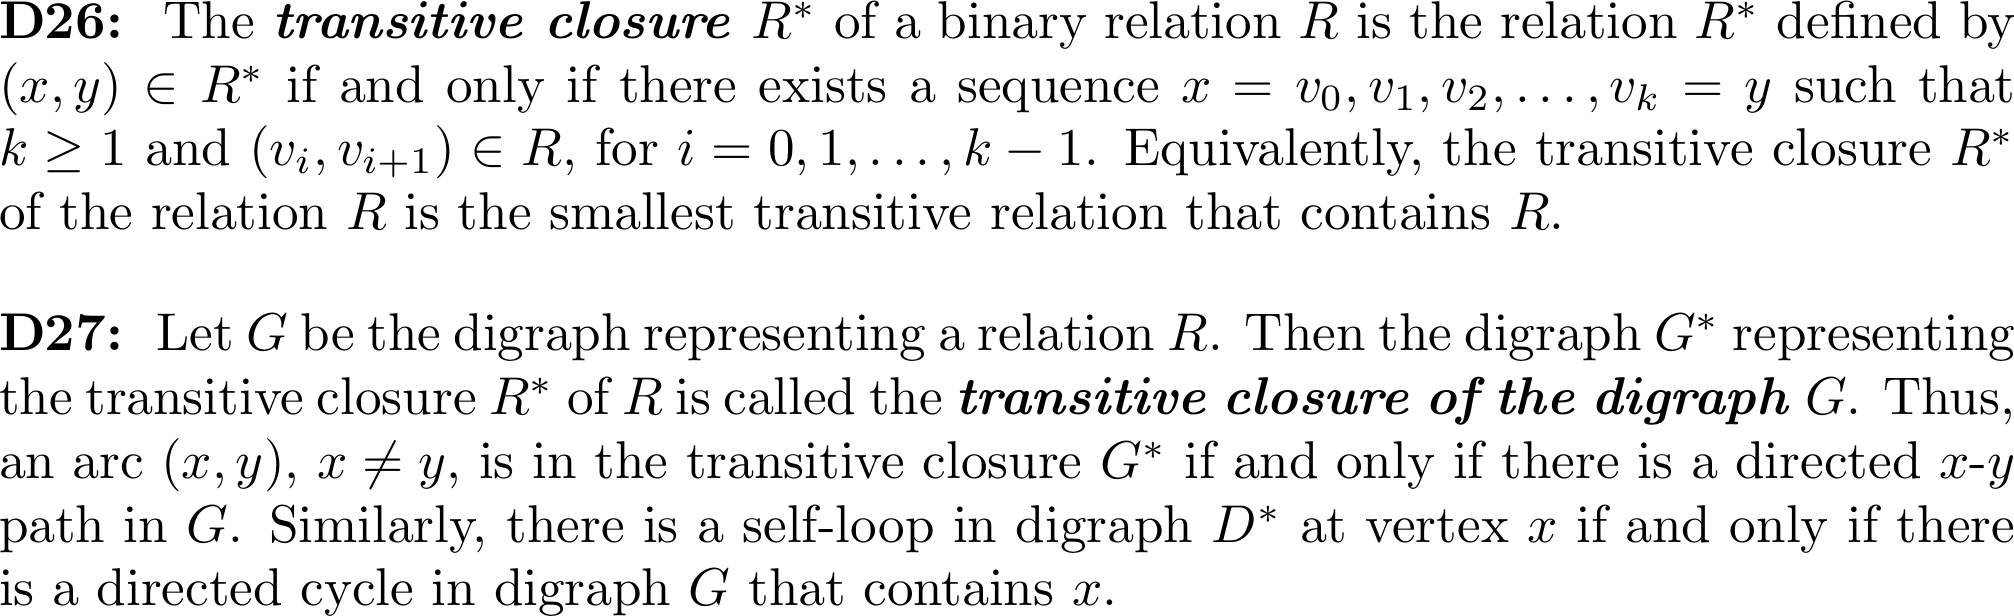
\includegraphics[width=.95\linewidth]{../img/grapht1.png}}
    \normalcolor%\caption{aus \cite[Seite 172]{gross2013handbook}}
\end{figure}

Oder kurz zusammengefasst: die transitive Hülle eines gerichteten Graphens $G$ ist wiederum ein gerichteter Graph $G^*$, der von jedem Knoten einen Bogen zu allen von diesem Knoten aus in $G$ erreichbaren Nachbarn besitzt. 

\newpage

In \cite[Seite 172]{gross2013handbook} ist hierzu folgendes Beispiel dargestellt:

\begin{figure}[H]
    \centering
    \setlength{\fboxsep}{10pt}\color{black!20}\fbox{
    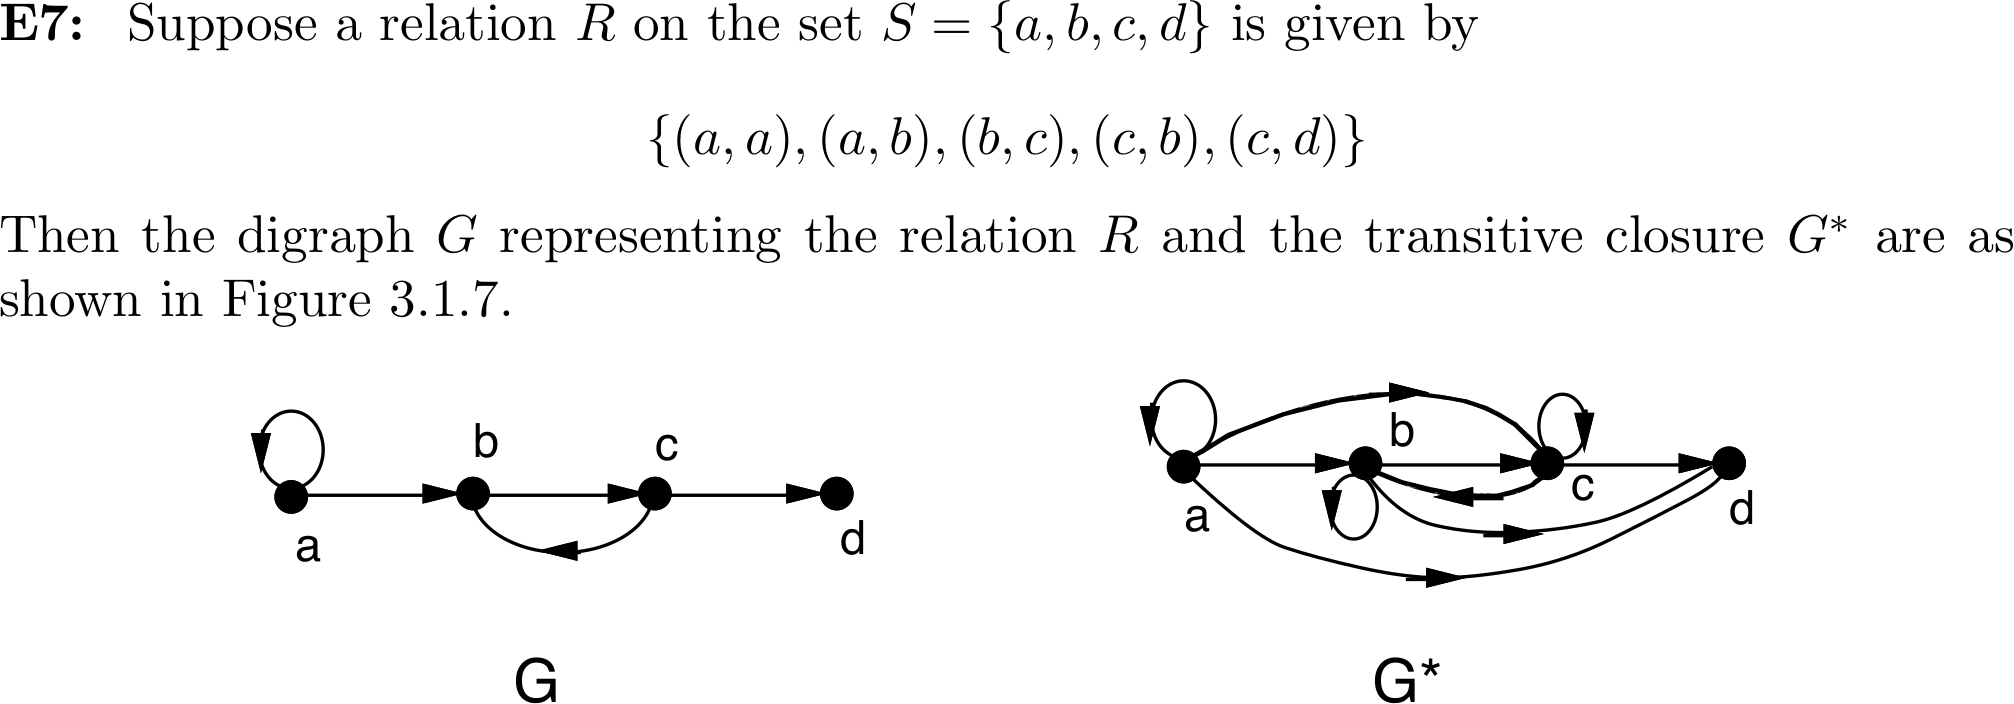
\includegraphics[width=.95\linewidth]{../img/grapht2.png}}
    \normalcolor%\caption{aus \cite[Seite 172]{gross2013handbook}}
\end{figure}

Es gibt mehrere Verfahren, um die transitive Hülle zu bestimmen. Es werden nun zwei Algorithmen vorgestellt, die anhand ihrer primären Suchrichtung benannt sind.

Wie in den Graphen dargestellt, läuft die \emph{horizontale} Suche primär über die Versionen -- mit jeweils einzelnen Kodes. Die \emph{vertikale} Suche läuft primär über die Kodes -- das heißt es werden zuerst alle Kodes einer Version gelesen.

\subsection{Horizontale Suche}

Ein intuitives Verfahren die transitive Hülle zu bestimmen wird in \cite[Seite 200]{jakobsson1991mixed} so beschrieben:

\begin{figure}[H]
    \centering
    \setlength{\fboxsep}{10pt}\color{black!20}\fbox{
    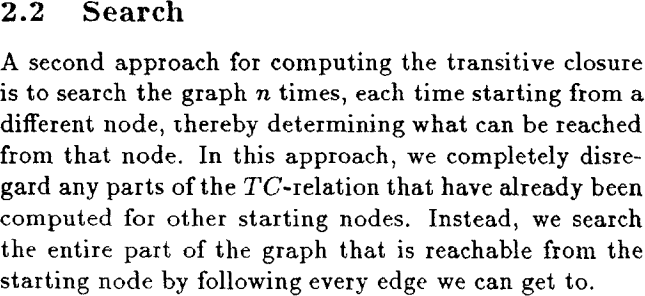
\includegraphics[width=.6\linewidth]{../img/search.png}}
    \normalcolor%\caption{aus \cite[Seite 200]{jakobsson1991mixed}}
    \vspace{-1em}
\end{figure}

Ähnlich wie im vorherigen Abschnitt für den Kode M21.6 dargestellt, werden also einfach ausgehend von einem Knoten so viele Suchen gestartet bis keine benachbarten Knoten mehr gefunden werden -- oder im Anwendungsfall der Umsteiger bis alle Versionen verarbeitet wurden.

Vorher erzielte Ergebnisse für andere Knoten, beziehungsweise Kodes, werden ignoriert. Das hieße im Beispiel oben, dass eine rückwärts chronologische Suche nach Umsteigern von M21.60 und M21.61 der ICD-10-GM Version ab dem Vorgänger M21.6 der Version 2014 zweimal exakt gleich ablaufen würde. 

Der Pseudocode für diese Vorgehensweise:

\begin{comment}
\begin{centernss}
\begin{struktogramm}(95,50)[test]
\assign{%
\begin{declaration}[Parameter:]
\description{\pVar{iPar}}{ an \pKey{int} parameter with the meaning described here}
\end{declaration}
\begin{declaration}[local Variables:]
\description{\pVar{iVar}}{an \pKey{int} variable with the meaning
described here}
\description{\pVar{dVar}}{a \pKey{double} variable with the
meaning described here}
\end{declaration}
}
\end{struktogramm}
\end{centernss}

\newpage
\end{comment}

%\subsection{SearchHorizontal}

\newpara{searchHorizontal}

Funktionsparameter:

\begin{comment}
\begin{itemize}
\item \texttt{system} \newline Das Kodiersystem, also zum Beispiel \texttt{icd10gm} oder \texttt{ops}. 
\item \texttt{version} \newline Version, beziehungsweise Jahrgang. 
\item \texttt{code} \newline Kode, nach dem gesucht wird. 
\end{itemize}
\end{comment}

\begin{itemize}
\item \texttt{\$system}, \texttt{\$version}, \texttt{\$code} \newline 
Wie Funktion readData, siehe Unterabschnitt \ref{function-read-data}.
\end{itemize}

Lokale Variable:

\begin{itemize}
\item \texttt{\$data} \hspace{2em} Rückgabewert, initial: leer.
\newline Eine assoziative Datenstruktur mit Key \texttt{fwd} $\Rightarrow$ Umsteiger, die chronologisch vorwärts von dem Suchkode erreichbar sind und \texttt{rev} $\Rightarrow$ chronologisch rückwärts. \\
\end{itemize}

\begin{comment}
\begingroup
\renewcommand{\arraystretch}{1.2}
\setlength{\tabcolsep}{12pt}
\begin{tabular}{|c|c|c|c|c|c|c|c|}
\hline
 & 2024 & 2023 & \dots & 2004 & 2.0 & 1.3 & \\
\hline
\end{tabular}
\endgroup
\end{comment}

\struktogrammAO{24}
{
\assign[\heightNS]{\$data[ 'fwd' ] = searchHorizontalRecursion (\$system, \$version, \$code, true)}
\assign[\heightNS]{\$data[ 'rev' ] = searchHorizontalRecursion (\$system, \$version, \$code, false)}
\return[\heightNS]{RETURN \$data}
}

\struktkommentar{Ausgehend von einem gegebenen Kodiersystem, Version, Kode wird chronologisch vorwärts und rückwärts eine rekursive Suche über alle Versionen gestartet.}

%\subsection{SearchHorizontalRecursion}

\newpara{searchHorizontalRecursion}

Funktionsparameter:

\begin{itemize}
\item \texttt{\$system}, \texttt{\$version}, \texttt{\$code} \newline Wie searchHorizontal. 
\item \texttt{\$chronological}
\newline Bestimmt die Suchrichtung. TRUE: chronologisch vorwärts und FALSE: rückwärts. 
\end{itemize}

Lokale Variablen:

\begin{itemize}
\item \texttt{\$data} \hspace{2em} Rückgabewert, initial: leer.
\newline Eine mehrdimensionale, assoziative Datenstruktur, die die Ergebnisse der rekursiven Suche enthält. Gefundene Umsteiger werden als Liste mit dem Key \texttt{umsteiger} gespeichert; zusätzlich zu den Listen wird auch die Versionen vorher und nachher notiert. Jeder einzelne Umsteiger-Eintrag enthält wiederum die Informationen zur automatischen Überleitbarkeit, sowie die Titel der Kodes vorher und nachher. Falls ein Umsteiger weitere Umsteiger hat, werden diese unter einem Key \texttt{recursion} abgelegt und die Suche fortgesetzt. Das heißt unter \texttt{recursion} ist das gleiche Datenkonstrukt nochmal enthalten. Ein Beispielergebnis für M21.6 befindet sich im Anhang \ref{search-horizontal-example}.
\item \texttt{\$otherVersion} \newline Die Version, zu der die Umsteiger ermittelt werden; \texttt{\$version} $\rightarrow$ \texttt{\$otherVersion}. 
\item \texttt{\$otherCode} \newline Die Spalte im Umsteiger-Eintrag, zu der der aktuelle Kode übergeleitet wird.
\item \texttt{\$readType} \newline Auf welche Art die Daten gelesen werden; siehe \texttt{readData}.
\item \texttt{\$umsteiger}, \texttt{\$entry} \newline Liste der Umsteiger, Schleifenvariable: Umsteiger-Eintrag.
\item \texttt{\$recursion} \newline Ergebnis des rekursiven Funktionsaufrufs bei gefundenen Umsteigern. \\
\end{itemize}

\struktogrammAO{35}{
    \ifthenelse[10]{1}{1}{IF \$chronological}{Y}{N}
        \assign[\heightNS]{\$otherVersion = \newline nextNewerVersion(\$system, \$version)}
        \assign[\heightNS]{\$readType = 'umsteiger\_join\_alt'}
        \assign[\heightNS]{\$otherCode = 'new'}
    \change
        \assign[\heightNS]{\$otherVersion = \newline nextOlderVersion(\$system, \$version)}
        \assign[\heightNS]{\$readType = 'umsteiger\_join'}
        \assign[\heightNS]{\$otherCode = 'old'}
    \ifend
}

\struktkommentar{Lokale Variablen werden anhand der Suchrichtung unterschiedlich belegt.}

\struktogrammAO{16}{
    \ifthenelse[10]{5}{1}{IF empty(\$version) OR empty(\$otherVersion)}{Y}{}
        \return[\heightNS]{RETURN \$data}
    \change
    \ifend
}

\struktkommentar{Falls es in der Suchrichtung keine weitere Version mehr gibt, endet die Rekursion.}

\struktogrammAO{27}{
    \assign[\heightNS]{\$umsteiger = readData(\$system, \$version, \$code, \$readType)}
    \ifthenelse[10]{5}{1}{IF empty(\$umsteiger)}{Y}{}
        \return[\heightNS]{RETURN \newline searchHorizontalRecursion(\$type, \$otherVersion, \$code, \$chronological)}
    \change
    \ifend
}

\struktkommentar{Die Umsteiger zwischen den Versionen im aktuellen Rekursionsschritt werden ermittelt. Falls es keine gibt --also keine, die eine Veränderung ausdrücken -- dann wird die Rekursion mit der nächsten Version fortgesetzt.}

%\texttt{readData ('icd10gm', '2014', 'M21.4', 'kodes')} 

\struktogrammAO{54}{
    \while[\heightNS]{FOREACH \$entry IN \$umsteiger}
        \ifthenelse[10]{5}{1}{IF \$entry[ \$otherCode ] IS NOT 'UNDEF'}{Y}{}
            \assign[\heightNS]{\$recursion = searchHorizontalRecursion \newline (\$system, \$version, \$entry[ \$otherCode ], \$chronological)}
            \ifthenelse[10]{4}{1}{IF NOT empty(\$recursion)}{Y}{}
                \assign[\heightNS]{\$entry[ 'recursion' ] = \$recursion}
            \change
            \ifend
        \change
        \ifend
        \assign[\heightNS]{\$data[ 'umsteiger' ][ ] = \$entry}
    \whileend
}

\struktkommentar{Für jeden Umsteiger wird die Rekursion mit dem veränderten Kode fortgesetzt. Allerdings nur falls dieser nicht UNDEF ist, weil es sich dann um einen entfernten oder neu hinzugefügten Kode handelt. Also wenn wie im Beispiel der M21.6 der ICD-10-GM Version 2013 die Umsteiger [ M21.60, M21.67, M21.87 ] in der Version 2012 hat, dann wird die Suche in die rückwärts chronologische Richtung mit diesen drei Kodes fortgesetzt statt mit M21.6. Die Ergebnisse dieser Verzweigung, sofern vorhanden, werden abgespeichert mit dem Key \texttt{recursion} zusätzlich zu jedem Umsteiger-Eintrag. Die Liste aller Umsteiger-Einträge, inklusive der UNDEF-Umsteiger, wird in das Ergebnis mit dem Key \texttt{umsteiger} aufgenommen.}

\struktogrammAO{23}{
    \assign[\heightNS]{\$data[ 'version' ] = \$version}
    \assign[\heightNS]{\$data[ 'other' ] = \$otherVersion}
    \return[\heightNS]{RETURN \$data}
}

\struktkommentar{Falls es Umsteiger für einen Kode gibt, werden zusätzlich die Versionen vorher und nachher gespeichert. Dann endet auch hier die Rekursion.}

Anhang \ref{search-horizontal-example} enthält das Ergebnis im JSON-Format für den Beispielaufruf der horizontale Suche für M21.6, Version 2014
%\texttt{searchHorizontal('icd10gm', '2014', 'M21.6')}
entsprechend der Abbildung \ref{img-m21-6}.

\begin{comment}
\struktogrammA{200}{searchUmsteigerHorizontal\_recursion
}{
    \assign[\heightNS]{ret = [ ]}
    \ifthenelse[10]{3}{1}{IF version === ' '}{TRUE}{FALSE}
        \return[\heightNS]{RETURN ret}
    \change
    \ifend
    \ifthenelse[10]{1}{1}{IF chronological}{TRUE}{FALSE}
        \assign[\heightNS]{other = nextNewerVersion(type, version)}
        \assign[\heightNS]{table = 'umsteiger\_join\_rev'}
        \assign[\heightNS]{which = 'new'}
    \change
        \assign[\heightNS]{other = nextOlderVersion(type, version)}
        \assign[\heightNS]{table = 'umsteiger\_join'}
        \assign[\heightNS]{which = 'old'}
    \ifend
    \ifthenelse[10]{3}{1}{IF other === ' '}{TRUE}{FALSE}
        \return[\heightNS]{RETURN ret}
    \change
    \ifend
    \assign[\heightNS]{umsteiger = readData(type, table, version, year, other, code)}
    \ifthenelse[10]{3}{1}{IF empty(umsteiger)}{TRUE}{FALSE}
        \return[\heightNS]{RETURN searchHorizontalRec(type, other, code, chronological)}
    \change
    \ifend
    \assign[\heightNS]{data = [ ]}
    \while[\heightNS]{FOREACH item IN umsteiger}
        \assign[\heightNS]{code = item[which]}
        \ifthenelse[10]{5}{1}{IF code !== 'UNDEF'}{TRUE}{FALSE}
            \assign[\heightNS]{recursion = searchHorizontalRec(type, other, search, chronological)}
            \ifthenelse[10]{4}{1}{IF NOT empty(recursion)}{TRUE}{FALSE}
                \assign[\heightNS]{item['recursion'] = recursion}
            \change
            \ifend
        \change
        \ifend
        \assign[\heightNS]{data[ ] = item}
    \whileend
    \assign[\heightNS]{ret['umsteiger'] = data}
    \assign[\heightNS]{ret['version'] = version}
    \assign[\heightNS]{ret['other'] = other}
    \return[\heightNS]{RETURN ret}
}
\end{comment}

\begin{comment}
{\small
\begin{struktogramm}(170,200)[searchUmsteigerHorizontal\_recursion]
    \assign[\heightNS]{ret = [ ]}
    \ifthenelse[10]{3}{1}{IF version === ' '}{TRUE}{FALSE}
        \return[\heightNS]{RETURN ret}
    \change
    \ifend
    \ifthenelse[10]{1}{1}{IF chronological}{TRUE}{FALSE}
        \assign[\heightNS]{other = nextNewerVersion(type, version)}
        \assign[\heightNS]{table = 'umsteiger\_join\_rev'}
        \assign[\heightNS]{which = 'new'}
    \change
        \assign[\heightNS]{other = nextOlderVersion(type, version)}
        \assign[\heightNS]{table = 'umsteiger\_join'}
        \assign[\heightNS]{which = 'old'}
    \ifend
    \ifthenelse[10]{3}{1}{IF other === ' '}{TRUE}{FALSE}
        \return[\heightNS]{RETURN ret}
    \change
    \ifend
    \assign[\heightNS]{umsteiger = readData(type, table, version, year, other, code)}
    \ifthenelse[10]{3}{1}{IF empty(umsteiger)}{TRUE}{FALSE}
        \return[\heightNS]{RETURN searchHorizontalRec(type, other, code, chronological)}
    \change
    \ifend
    \assign[\heightNS]{data = [ ]}
    \while[\heightNS]{FOREACH item IN umsteiger}
        \assign[\heightNS]{code = item[which]}
        \ifthenelse[10]{5}{1}{IF code !== 'UNDEF'}{TRUE}{FALSE}
            \assign[\heightNS]{recursion = searchHorizontalRec(type, other, search, chronological)}
            \ifthenelse[10]{4}{1}{IF NOT empty(recursion)}{TRUE}{FALSE}
                \assign[\heightNS]{item['recursion'] = recursion}
            \change
            \ifend
        \change
        \ifend
        \assign[\heightNS]{data[ ] = item}
    \whileend
    \assign[\heightNS]{ret['umsteiger'] = umsteiger}
    \assign[\heightNS]{ret['version'] = version}
    \assign[\heightNS]{ret['other'] = other}
    \return[\heightNS]{RETURN ret}
\end{struktogramm}
}
\end{comment}

% Bei UNDEF: array_unshift($umsteiger_out, $find);

\subsection{Vertikale Suche}
\label{vert-search}

Wie bereits erwähnt beginnt der Algorithmus der horizontalen Suche für jeden Kode ohne Vorkenntnisse über schon getätigte Aufrufe. Wenn die Umsteiger für alle Kodes einer Version --beziehungsweise eines ganzen Kodiersystems-- gefunden werden sollen, ist diese Vorgehensweise nicht effizient. 

Besonders für gerichtete Graphen ist allerdings Purdoms Algorithmus gut geeignet, um die transitive Hülle zu bestimmen, wie in \cite[Seite 77]{dar1993augmenting} beschrieben. Folgende kurze Zusammenfassung des Algorithmus basiert auf dieser Beschreibung, sowie auf \cite{purdom1970transitive} selbst: 

\begin{enumerate}
\item Ausgehend von einem Graphen $G$: Bestimme die stark zusammenhängenden Komponenten ($SCC$) in $G$ und vereinige diese in jeweils einen einzelnen Knoten. Das Ergebnis ist ein zyklenfreier, verdichteter Graph $G_c$.  %Let the original graph be G. Compute the strongly connected components in G, and collapse each one into a single node. Let the resulting acyclic condensation graph be Gc.
\item Sortiere $G_c$ topologisch. % Obtain a topological sort on Gc.
\item Ermittele die transitive Hülle von $G_c$ über dessen Adjazenzlisten in rückwärts topologischer Reihenfolge. % (Bestimme die erreichbaren Knoten über Adjazenzlisten) % Compute the transitive closure of Gc by expanding successor lists in reverse topological order.
\item Bestimme die transitive Hülle des ursprünglichen Graphens $G$ über die Nachbarschaftslisten der stark zusammenhängenen Komponenten in $G_c$: ein Knoten $y$ ist ein erreichbarer Nachbar von Knoten $x$, falls $SCC(y) = SCC(x)$ oder falls $SCC(y)$ ein erreichbarer Nachbar von $SCC(x)$ ist. % Compute the successor lists of the nodes in the original graph G from the successor lists of their respective SCCs: a node y is a successor of node x in G if SCC(y) = SCC(x) or SSC(y) is a succcessor of SCC(x) in Gc. 
\end{enumerate}

Die Vereinigung der stark zusammenhängenden Komponenten aus Schritt eins wird in \cite{purdom1970transitive} wie folgt dargestellt: 

%\begin{figure}[H]
%    \centering
%    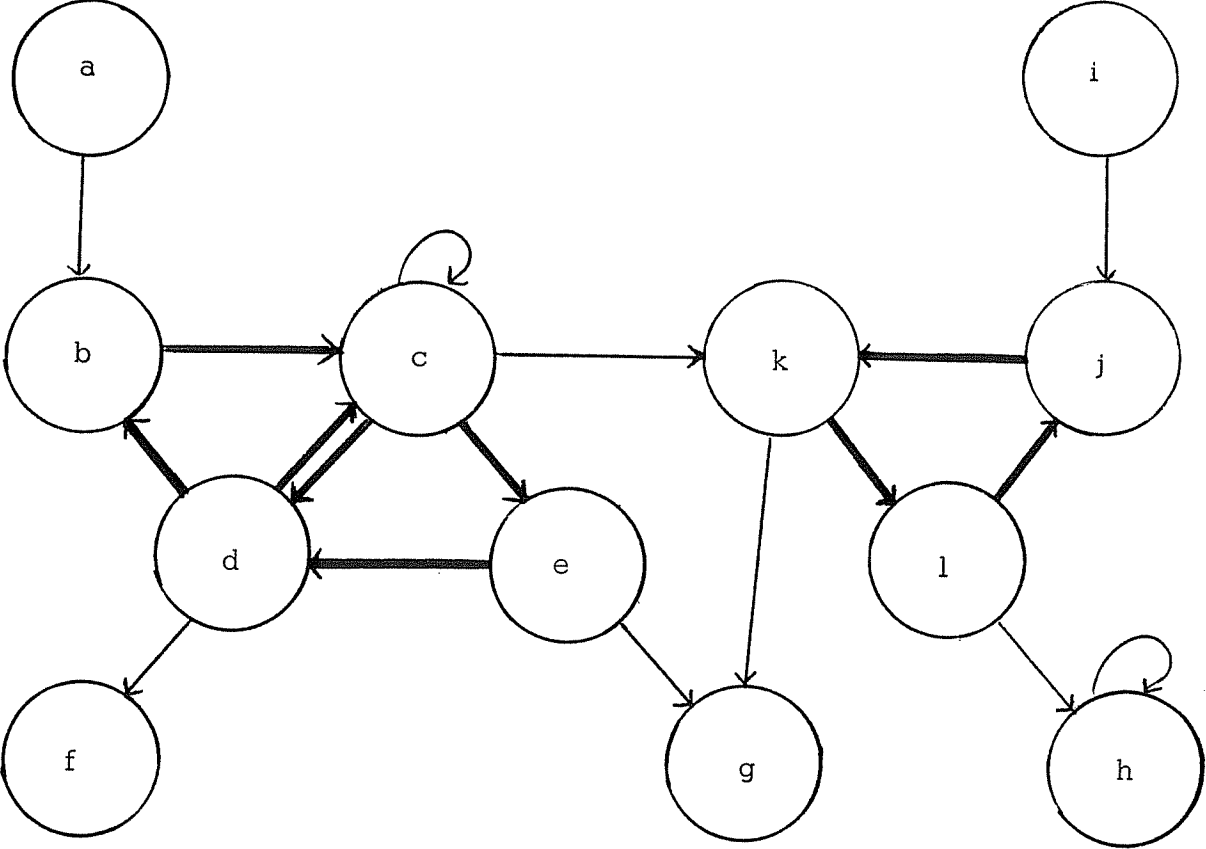
\includegraphics[width=.6\linewidth]{../img/purdom_g1.png}
%    \caption{Beispiel Graph $G$ von \cite[Seite 78]{purdom1970transitive}}
%\end{figure}

\begin{figure}[H]
    \centering
    \setlength{\fboxsep}{10pt}\color{black!20}\fbox{
    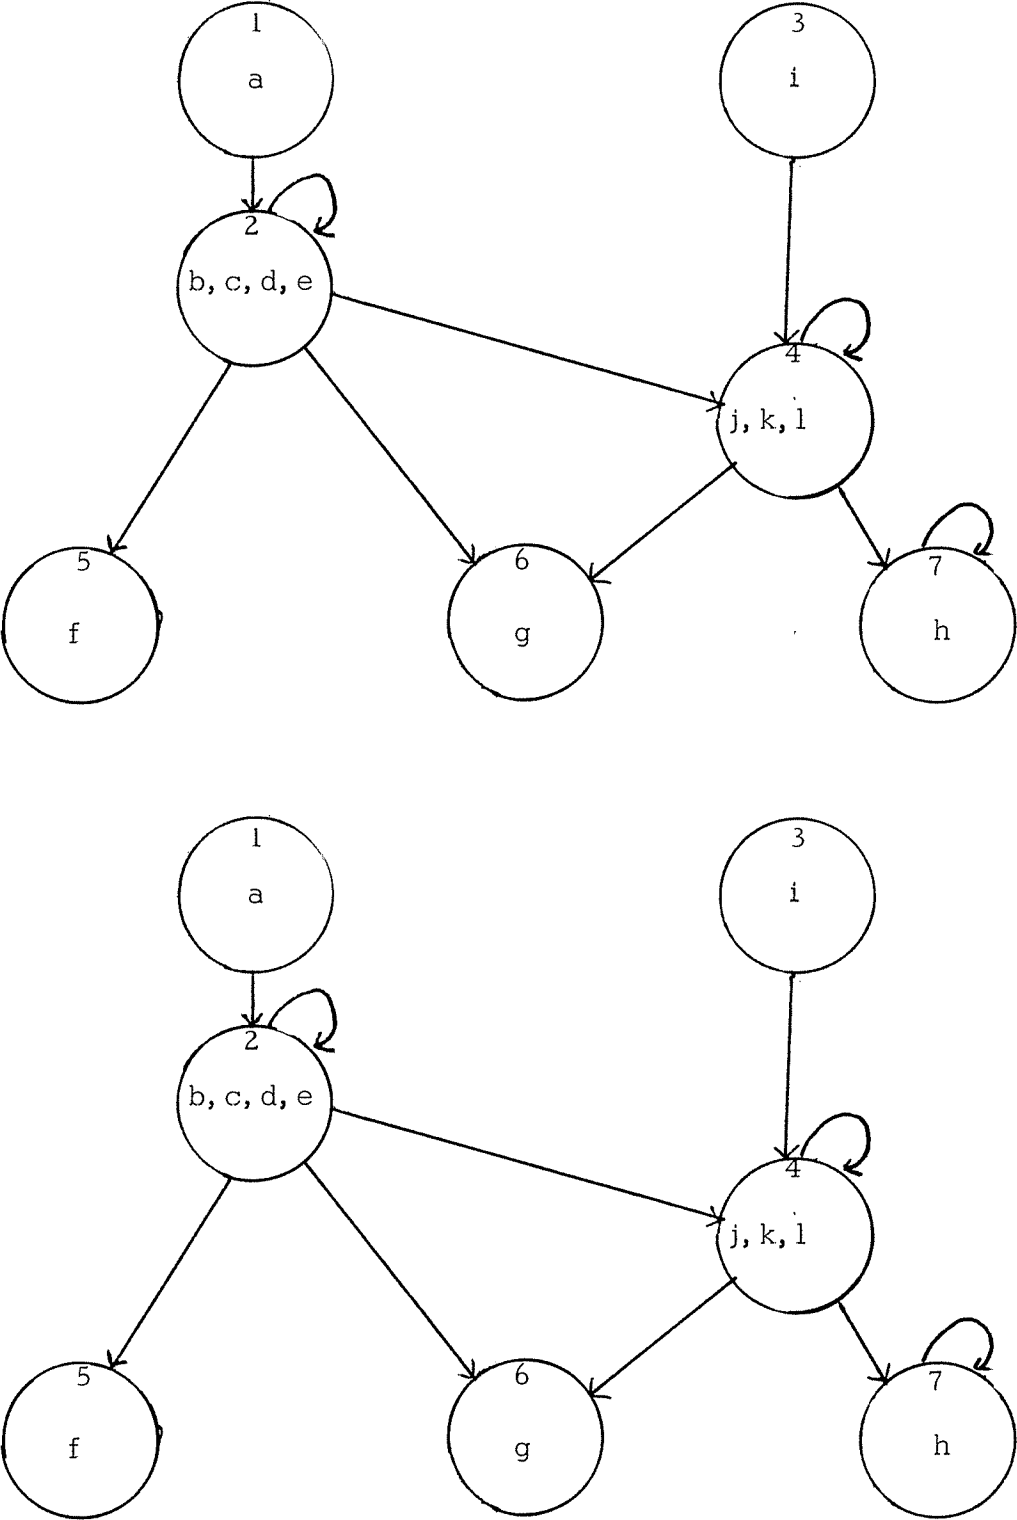
\includegraphics[width=.59\linewidth]{../img/purdom_g.png}}
    \normalcolor\caption{Beispielgraph $G$ und Vereinigung der stark zusammenhängenden Komponenten aus \cite[Seite 78]{purdom1970transitive}.}\vspace{-1.9em}
\end{figure}

Die hier vorgestellte vertikale Suche nach Umsteigern entspricht nicht ganz Purdoms Algorithmus. Sie weicht in mehreren Punkten ab:

\begin{itemize}
\item Die topologische Sortierung aus Schritt zwei in der Anwendung der Suche nach Umsteigern ist nicht notwendig, weil die Versionen immer in einer bestimmte Richtung verglichen werden und die Kodes sich nur zwischen zwei Versionen ändern können. Die Daten sind also schon implizit topologisch sortiert.
\item Ebenfalls ist nicht notwendig, die komplette transitiven Hülle zu ermitteln, sondern nur wie Kodes der Startversion in die Zielversion übergeleitet werden. Die Zwischenergebnisse werden trotzdem gespeichert. 
\item Auch bei der Suche nach Umsteigern nur mit Veränderungen ist es möglich, anders als bei den Knoten in einem Graphen, dass Kodes mehrmals vorkommen. Zum Beispiel gibt es G83.3 in ICD-10-GM nicht zwischen Version 2017 und 2005, aber schon davor und danach.  
\end{itemize} 

Trotzdem basiert die vertikale Suche wesentlich auf zwei Besonderheiten von Purdoms Algorithmus, die in \cite[Seite 76f]{dar1993augmenting} hervorgehoben werden:

\begin{figure}[H]
    \centering
    \setlength{\fboxsep}{10pt}\color{black!20}\fbox{
    
\includegraphics[width=.99\linewidth]{../img/purdom_r.png}}
    \normalcolor%\caption{aus \cite[Seite 76f]{dar1993augmenting}}
\end{figure}

Konkret bedeuten diese Besonderheiten für die Umsteiger-Suche:

\begin{enumerate}
\item Topologisch rückwärts gerichtete Vorgehensweise:\newline So ist zum Beispiel bei der Suche nach den Umsteigern eines ICD-GM-10 Kodes der Version 1.3 die Reihenfolge, in der die anderen Versionen abgearbeitet werden: 2024, 2023, 2022 und so weiter. Oder anders ausgedrückt: Wenn die Überleitungen in chronologischer Reihenfolge bestimmt werden sollen, dann läuft die vertikale Suche umgekehrt, also chronologisch rückwärts. 
\item Vereinigung der stark zusammenhängenden Komponenten:\newline Nach jedem Schritt über eine Version, wird geprüft, ob ein neu gefundener Umsteiger eine Überleitung in einen Kode enthält, der bereits in den davor abgearbeiteten Versionen als Umsteiger vorkommt. Falls ja, dann werden diese Umsteiger vereinigt, das heißt die Zwischenschritte werden zu einem Schritt zusammengefügt. 
\end{enumerate}

\ \\

Abbildung \ref{merge-illustrated} auf der nächsten Seite zeigt ein einfaches Beispiel für die Vereinigung: 

Angenommen ein abstraktes System hat Umsteiger von der Version 1.0 auf 2.0: $A$$\rightarrow$$B$ und $M$$\rightarrow$$N$, sowie von Version 2.0 auf 3.0: $B$$\rightarrow$$C$. Wenn nun in chronologischer Reihenfolge 1.0$\rightarrow$2.0$\rightarrow$3.0 Umsteiger ermittelt werden sollen, erfolgt die Suche sowie Vereinigung gefundener Umsteiger in umgekehrter Reihenfolge. Das heißt wenn im Schritt 3.0$\leftarrow$2.0 der Umsteiger $C$$\leftarrow$$B$ gefunden wird, dann wird danach bei der Vereinigung mit Version 1.0 der Umsteiger $B$$\leftarrow$$A$ in $C$$\leftarrow$$A$ umgewandelt. $A$ in Version 1.0 entspricht $C$ in Version 3.0. 

Falls es Verzweigungen gibt, also es mehrere Umsteiger für einen Kode gibt, dann werden entsprechend Listen vereinigt. Ein reales Beispiel dazu folgt später. 

\begin{figure}[H]
    \centering\Huge%\sffamily
    \resizebox{.75\linewidth}{!}{% Graphic for TeX using PGF
% Title: /home/simon/jacuke_ma/tex/dia/merge.dia
% Creator: Dia v0.97+git
% CreationDate: Mon Oct 28 09:00:01 2024
% For: simon
% \usepackage{tikz}
% The following commands are not supported in PSTricks at present
% We define them conditionally, so when they are implemented,
% this pgf file will use them.
\ifx\du\undefined
  \newlength{\du}
\fi
\setlength{\du}{15\unitlength}
\begin{tikzpicture}[even odd rule]
\pgftransformxscale{1.000000}
\pgftransformyscale{-1.000000}
\definecolor{dialinecolor}{rgb}{0.000000, 0.000000, 0.000000}
\pgfsetstrokecolor{dialinecolor}
\pgfsetstrokeopacity{1.000000}
\definecolor{diafillcolor}{rgb}{1.000000, 1.000000, 1.000000}
\pgfsetfillcolor{diafillcolor}
\pgfsetfillopacity{1.000000}
\pgfsetlinewidth{0.100000\du}
\pgfsetdash{}{0pt}
\pgfsetmiterjoin
\pgfsetbuttcap
{\pgfsetcornersarced{\pgfpoint{0.000000\du}{0.000000\du}}\definecolor{diafillcolor}{rgb}{1.000000, 1.000000, 1.000000}
\pgfsetfillcolor{diafillcolor}
\pgfsetfillopacity{0.117647}
\fill (-26.000000\du,-33.000000\du)--(-26.000000\du,-6.000000\du)--(29.000000\du,-6.000000\du)--(29.000000\du,-33.000000\du)--cycle;
}{\pgfsetcornersarced{\pgfpoint{0.000000\du}{0.000000\du}}\definecolor{dialinecolor}{rgb}{1.000000, 1.000000, 1.000000}
\pgfsetstrokecolor{dialinecolor}
\pgfsetstrokeopacity{1.000000}
\draw (-26.000000\du,-33.000000\du)--(-26.000000\du,-6.000000\du)--(29.000000\du,-6.000000\du)--(29.000000\du,-33.000000\du)--cycle;
}\pgfsetlinewidth{0.100000\du}
\pgfsetdash{}{0pt}
\pgfsetroundjoin
\pgfsetbuttcap
{\pgfsetcornersarced{\pgfpoint{2.000000\du}{2.000000\du}}\definecolor{diafillcolor}{rgb}{1.000000, 1.000000, 1.000000}
\pgfsetfillcolor{diafillcolor}
\pgfsetfillopacity{1.000000}
\fill (-9.000000\du,-27.000000\du)--(-9.000000\du,-7.000000\du)--(5.000000\du,-7.000000\du)--(5.000000\du,-27.000000\du)--cycle;
}{\pgfsetcornersarced{\pgfpoint{2.000000\du}{2.000000\du}}\definecolor{dialinecolor}{rgb}{0.411765, 0.411765, 0.411765}
\pgfsetstrokecolor{dialinecolor}
\pgfsetstrokeopacity{1.000000}
\draw (-9.000000\du,-27.000000\du)--(-9.000000\du,-7.000000\du)--(5.000000\du,-7.000000\du)--(5.000000\du,-27.000000\du)--cycle;
}\pgfsetlinewidth{0.100000\du}
\pgfsetdash{}{0pt}
\pgfsetroundjoin
\pgfsetbuttcap
{\pgfsetcornersarced{\pgfpoint{2.000000\du}{2.000000\du}}\definecolor{diafillcolor}{rgb}{1.000000, 1.000000, 1.000000}
\pgfsetfillcolor{diafillcolor}
\pgfsetfillopacity{1.000000}
\fill (-25.000000\du,-27.000000\du)--(-25.000000\du,-7.000000\du)--(-11.000000\du,-7.000000\du)--(-11.000000\du,-27.000000\du)--cycle;
}{\pgfsetcornersarced{\pgfpoint{2.000000\du}{2.000000\du}}\definecolor{dialinecolor}{rgb}{0.411765, 0.411765, 0.411765}
\pgfsetstrokecolor{dialinecolor}
\pgfsetstrokeopacity{1.000000}
\draw (-25.000000\du,-27.000000\du)--(-25.000000\du,-7.000000\du)--(-11.000000\du,-7.000000\du)--(-11.000000\du,-27.000000\du)--cycle;
}\pgfsetlinewidth{0.100000\du}
\pgfsetdash{}{0pt}
\definecolor{diafillcolor}{rgb}{1.000000, 1.000000, 1.000000}
\pgfsetfillcolor{diafillcolor}
\pgfsetfillopacity{1.000000}
\pgfpathellipse{\pgfpoint{-15.000000\du}{-23.000000\du}}{\pgfpoint{2.000000\du}{0\du}}{\pgfpoint{0\du}{2.000000\du}}
\pgfusepath{fill}
\definecolor{dialinecolor}{rgb}{0.000000, 0.000000, 0.000000}
\pgfsetstrokecolor{dialinecolor}
\pgfsetstrokeopacity{1.000000}
\pgfpathellipse{\pgfpoint{-15.000000\du}{-23.000000\du}}{\pgfpoint{2.000000\du}{0\du}}{\pgfpoint{0\du}{2.000000\du}}
\pgfusepath{stroke}
% setfont left to latex
\definecolor{dialinecolor}{rgb}{0.000000, 0.000000, 0.000000}
\pgfsetstrokecolor{dialinecolor}
\pgfsetstrokeopacity{1.000000}
\definecolor{diafillcolor}{rgb}{0.000000, 0.000000, 0.000000}
\pgfsetfillcolor{diafillcolor}
\pgfsetfillopacity{1.000000}
\node[anchor=base,inner sep=0pt, outer sep=0pt,color=dialinecolor] at (-15.000000\du,-22.354276\du){B};
\pgfsetlinewidth{0.200000\du}
\pgfsetdash{}{0pt}
\pgfsetbuttcap
{
\definecolor{diafillcolor}{rgb}{0.000000, 0.000000, 0.000000}
\pgfsetfillcolor{diafillcolor}
\pgfsetfillopacity{1.000000}
% was here!!!
\pgfsetarrowsend{stealth}
\definecolor{dialinecolor}{rgb}{0.000000, 0.000000, 0.000000}
\pgfsetstrokecolor{dialinecolor}
\pgfsetstrokeopacity{1.000000}
\draw (-17.044922\du,-23.000000\du)--(-18.955078\du,-23.000000\du);
}
\pgfsetlinewidth{0.100000\du}
\pgfsetdash{}{0pt}
\definecolor{diafillcolor}{rgb}{1.000000, 1.000000, 1.000000}
\pgfsetfillcolor{diafillcolor}
\pgfsetfillopacity{1.000000}
\pgfpathellipse{\pgfpoint{-21.000000\du}{-23.000000\du}}{\pgfpoint{2.000000\du}{0\du}}{\pgfpoint{0\du}{2.000000\du}}
\pgfusepath{fill}
\definecolor{dialinecolor}{rgb}{0.000000, 0.000000, 0.000000}
\pgfsetstrokecolor{dialinecolor}
\pgfsetstrokeopacity{1.000000}
\pgfpathellipse{\pgfpoint{-21.000000\du}{-23.000000\du}}{\pgfpoint{2.000000\du}{0\du}}{\pgfpoint{0\du}{2.000000\du}}
\pgfusepath{stroke}
% setfont left to latex
\definecolor{dialinecolor}{rgb}{0.000000, 0.000000, 0.000000}
\pgfsetstrokecolor{dialinecolor}
\pgfsetstrokeopacity{1.000000}
\definecolor{diafillcolor}{rgb}{0.000000, 0.000000, 0.000000}
\pgfsetfillcolor{diafillcolor}
\pgfsetfillopacity{1.000000}
\node[anchor=base,inner sep=0pt, outer sep=0pt,color=dialinecolor] at (-21.000000\du,-22.354276\du){C};
\pgfsetlinewidth{0.100000\du}
\pgfsetdash{}{0pt}
\definecolor{diafillcolor}{rgb}{1.000000, 1.000000, 1.000000}
\pgfsetfillcolor{diafillcolor}
\pgfsetfillopacity{1.000000}
\pgfpathellipse{\pgfpoint{1.000000\du}{-17.000000\du}}{\pgfpoint{2.000000\du}{0\du}}{\pgfpoint{0\du}{2.000000\du}}
\pgfusepath{fill}
\definecolor{dialinecolor}{rgb}{0.000000, 0.000000, 0.000000}
\pgfsetstrokecolor{dialinecolor}
\pgfsetstrokeopacity{1.000000}
\pgfpathellipse{\pgfpoint{1.000000\du}{-17.000000\du}}{\pgfpoint{2.000000\du}{0\du}}{\pgfpoint{0\du}{2.000000\du}}
\pgfusepath{stroke}
% setfont left to latex
\definecolor{dialinecolor}{rgb}{0.000000, 0.000000, 0.000000}
\pgfsetstrokecolor{dialinecolor}
\pgfsetstrokeopacity{1.000000}
\definecolor{diafillcolor}{rgb}{0.000000, 0.000000, 0.000000}
\pgfsetfillcolor{diafillcolor}
\pgfsetfillopacity{1.000000}
\node[anchor=base,inner sep=0pt, outer sep=0pt,color=dialinecolor] at (1.000000\du,-16.354276\du){A};
\pgfsetlinewidth{0.200000\du}
\pgfsetdash{}{0pt}
\pgfsetbuttcap
{
\definecolor{diafillcolor}{rgb}{0.000000, 0.000000, 0.000000}
\pgfsetfillcolor{diafillcolor}
\pgfsetfillopacity{1.000000}
% was here!!!
\pgfsetarrowsend{stealth}
\definecolor{dialinecolor}{rgb}{0.000000, 0.000000, 0.000000}
\pgfsetstrokecolor{dialinecolor}
\pgfsetstrokeopacity{1.000000}
\draw (-1.044922\du,-17.000000\du)--(-2.955078\du,-17.000000\du);
}
\pgfsetlinewidth{0.100000\du}
\pgfsetdash{}{0pt}
\definecolor{diafillcolor}{rgb}{1.000000, 1.000000, 1.000000}
\pgfsetfillcolor{diafillcolor}
\pgfsetfillopacity{1.000000}
\pgfpathellipse{\pgfpoint{-5.000000\du}{-17.000000\du}}{\pgfpoint{2.000000\du}{0\du}}{\pgfpoint{0\du}{2.000000\du}}
\pgfusepath{fill}
\definecolor{dialinecolor}{rgb}{0.000000, 0.000000, 0.000000}
\pgfsetstrokecolor{dialinecolor}
\pgfsetstrokeopacity{1.000000}
\pgfpathellipse{\pgfpoint{-5.000000\du}{-17.000000\du}}{\pgfpoint{2.000000\du}{0\du}}{\pgfpoint{0\du}{2.000000\du}}
\pgfusepath{stroke}
% setfont left to latex
\definecolor{dialinecolor}{rgb}{0.000000, 0.000000, 0.000000}
\pgfsetstrokecolor{dialinecolor}
\pgfsetstrokeopacity{1.000000}
\definecolor{diafillcolor}{rgb}{0.000000, 0.000000, 0.000000}
\pgfsetfillcolor{diafillcolor}
\pgfsetfillopacity{1.000000}
\node[anchor=base,inner sep=0pt, outer sep=0pt,color=dialinecolor] at (-5.000000\du,-16.354276\du){B};
\pgfsetlinewidth{0.100000\du}
\pgfsetdash{}{0pt}
\definecolor{diafillcolor}{rgb}{1.000000, 1.000000, 1.000000}
\pgfsetfillcolor{diafillcolor}
\pgfsetfillopacity{1.000000}
\pgfpathellipse{\pgfpoint{1.000000\du}{-11.000000\du}}{\pgfpoint{2.000000\du}{0\du}}{\pgfpoint{0\du}{2.000000\du}}
\pgfusepath{fill}
\definecolor{dialinecolor}{rgb}{0.000000, 0.000000, 0.000000}
\pgfsetstrokecolor{dialinecolor}
\pgfsetstrokeopacity{1.000000}
\pgfpathellipse{\pgfpoint{1.000000\du}{-11.000000\du}}{\pgfpoint{2.000000\du}{0\du}}{\pgfpoint{0\du}{2.000000\du}}
\pgfusepath{stroke}
% setfont left to latex
\definecolor{dialinecolor}{rgb}{0.000000, 0.000000, 0.000000}
\pgfsetstrokecolor{dialinecolor}
\pgfsetstrokeopacity{1.000000}
\definecolor{diafillcolor}{rgb}{0.000000, 0.000000, 0.000000}
\pgfsetfillcolor{diafillcolor}
\pgfsetfillopacity{1.000000}
\node[anchor=base,inner sep=0pt, outer sep=0pt,color=dialinecolor] at (1.000000\du,-10.354276\du){M};
\pgfsetlinewidth{0.200000\du}
\pgfsetdash{}{0pt}
\pgfsetbuttcap
{
\definecolor{diafillcolor}{rgb}{0.000000, 0.000000, 0.000000}
\pgfsetfillcolor{diafillcolor}
\pgfsetfillopacity{1.000000}
% was here!!!
\pgfsetarrowsend{stealth}
\definecolor{dialinecolor}{rgb}{0.000000, 0.000000, 0.000000}
\pgfsetstrokecolor{dialinecolor}
\pgfsetstrokeopacity{1.000000}
\draw (-1.044922\du,-11.000000\du)--(-2.955078\du,-11.000000\du);
}
\pgfsetlinewidth{0.100000\du}
\pgfsetdash{}{0pt}
\definecolor{diafillcolor}{rgb}{1.000000, 1.000000, 1.000000}
\pgfsetfillcolor{diafillcolor}
\pgfsetfillopacity{1.000000}
\pgfpathellipse{\pgfpoint{-5.000000\du}{-11.000000\du}}{\pgfpoint{2.000000\du}{0\du}}{\pgfpoint{0\du}{2.000000\du}}
\pgfusepath{fill}
\definecolor{dialinecolor}{rgb}{0.000000, 0.000000, 0.000000}
\pgfsetstrokecolor{dialinecolor}
\pgfsetstrokeopacity{1.000000}
\pgfpathellipse{\pgfpoint{-5.000000\du}{-11.000000\du}}{\pgfpoint{2.000000\du}{0\du}}{\pgfpoint{0\du}{2.000000\du}}
\pgfusepath{stroke}
% setfont left to latex
\definecolor{dialinecolor}{rgb}{0.000000, 0.000000, 0.000000}
\pgfsetstrokecolor{dialinecolor}
\pgfsetstrokeopacity{1.000000}
\definecolor{diafillcolor}{rgb}{0.000000, 0.000000, 0.000000}
\pgfsetfillcolor{diafillcolor}
\pgfsetfillopacity{1.000000}
\node[anchor=base,inner sep=0pt, outer sep=0pt,color=dialinecolor] at (-5.000000\du,-10.354276\du){N};
\pgfsetlinewidth{0.100000\du}
\pgfsetdash{}{0pt}
\pgfsetroundjoin
\pgfsetbuttcap
{\pgfsetcornersarced{\pgfpoint{2.000000\du}{2.000000\du}}\definecolor{diafillcolor}{rgb}{1.000000, 1.000000, 1.000000}
\pgfsetfillcolor{diafillcolor}
\pgfsetfillopacity{1.000000}
\fill (-22.000000\du,-32.000000\du)--(-22.000000\du,-28.000000\du)--(-14.000000\du,-28.000000\du)--(-14.000000\du,-32.000000\du)--cycle;
}{\pgfsetcornersarced{\pgfpoint{2.000000\du}{2.000000\du}}\definecolor{dialinecolor}{rgb}{0.411765, 0.411765, 0.411765}
\pgfsetstrokecolor{dialinecolor}
\pgfsetstrokeopacity{1.000000}
\draw (-22.000000\du,-32.000000\du)--(-22.000000\du,-28.000000\du)--(-14.000000\du,-28.000000\du)--(-14.000000\du,-32.000000\du)--cycle;
}% setfont left to latex
\definecolor{dialinecolor}{rgb}{0.000000, 0.000000, 0.000000}
\pgfsetstrokecolor{dialinecolor}
\pgfsetstrokeopacity{1.000000}
\definecolor{diafillcolor}{rgb}{0.000000, 0.000000, 0.000000}
\pgfsetfillcolor{diafillcolor}
\pgfsetfillopacity{1.000000}
\node[anchor=base,inner sep=0pt, outer sep=0pt,color=dialinecolor] at (-18.000000\du,-29.381708\du){3.0 – 2.0};
\pgfsetlinewidth{0.100000\du}
\pgfsetdash{}{0pt}
\pgfsetroundjoin
\pgfsetbuttcap
{\pgfsetcornersarced{\pgfpoint{2.000000\du}{2.000000\du}}\definecolor{diafillcolor}{rgb}{1.000000, 1.000000, 1.000000}
\pgfsetfillcolor{diafillcolor}
\pgfsetfillopacity{1.000000}
\fill (-6.000000\du,-32.000000\du)--(-6.000000\du,-28.000000\du)--(2.000000\du,-28.000000\du)--(2.000000\du,-32.000000\du)--cycle;
}{\pgfsetcornersarced{\pgfpoint{2.000000\du}{2.000000\du}}\definecolor{dialinecolor}{rgb}{0.411765, 0.411765, 0.411765}
\pgfsetstrokecolor{dialinecolor}
\pgfsetstrokeopacity{1.000000}
\draw (-6.000000\du,-32.000000\du)--(-6.000000\du,-28.000000\du)--(2.000000\du,-28.000000\du)--(2.000000\du,-32.000000\du)--cycle;
}% setfont left to latex
\definecolor{dialinecolor}{rgb}{0.000000, 0.000000, 0.000000}
\pgfsetstrokecolor{dialinecolor}
\pgfsetstrokeopacity{1.000000}
\definecolor{diafillcolor}{rgb}{0.000000, 0.000000, 0.000000}
\pgfsetfillcolor{diafillcolor}
\pgfsetfillopacity{1.000000}
\node[anchor=base,inner sep=0pt, outer sep=0pt,color=dialinecolor] at (-2.000000\du,-29.381708\du){2.0 – 1.0};
\pgfsetlinewidth{0.100000\du}
\pgfsetdash{}{0pt}
\pgfsetroundjoin
\pgfsetbuttcap
{\pgfsetcornersarced{\pgfpoint{2.000000\du}{2.000000\du}}\definecolor{diafillcolor}{rgb}{1.000000, 1.000000, 1.000000}
\pgfsetfillcolor{diafillcolor}
\pgfsetfillopacity{1.000000}
\fill (14.000000\du,-27.000000\du)--(14.000000\du,-7.000000\du)--(28.000000\du,-7.000000\du)--(28.000000\du,-27.000000\du)--cycle;
}{\pgfsetcornersarced{\pgfpoint{2.000000\du}{2.000000\du}}\definecolor{dialinecolor}{rgb}{0.411765, 0.411765, 0.411765}
\pgfsetstrokecolor{dialinecolor}
\pgfsetstrokeopacity{1.000000}
\draw (14.000000\du,-27.000000\du)--(14.000000\du,-7.000000\du)--(28.000000\du,-7.000000\du)--(28.000000\du,-27.000000\du)--cycle;
}\pgfsetlinewidth{0.100000\du}
\pgfsetdash{}{0pt}
\definecolor{diafillcolor}{rgb}{1.000000, 1.000000, 1.000000}
\pgfsetfillcolor{diafillcolor}
\pgfsetfillopacity{1.000000}
\pgfpathellipse{\pgfpoint{24.000000\du}{-17.000000\du}}{\pgfpoint{2.000000\du}{0\du}}{\pgfpoint{0\du}{2.000000\du}}
\pgfusepath{fill}
\definecolor{dialinecolor}{rgb}{0.000000, 0.000000, 0.000000}
\pgfsetstrokecolor{dialinecolor}
\pgfsetstrokeopacity{1.000000}
\pgfpathellipse{\pgfpoint{24.000000\du}{-17.000000\du}}{\pgfpoint{2.000000\du}{0\du}}{\pgfpoint{0\du}{2.000000\du}}
\pgfusepath{stroke}
% setfont left to latex
\definecolor{dialinecolor}{rgb}{0.000000, 0.000000, 0.000000}
\pgfsetstrokecolor{dialinecolor}
\pgfsetstrokeopacity{1.000000}
\definecolor{diafillcolor}{rgb}{0.000000, 0.000000, 0.000000}
\pgfsetfillcolor{diafillcolor}
\pgfsetfillopacity{1.000000}
\node[anchor=base,inner sep=0pt, outer sep=0pt,color=dialinecolor] at (24.000000\du,-16.354276\du){A};
\pgfsetlinewidth{0.200000\du}
\pgfsetdash{}{0pt}
\pgfsetbuttcap
{
\definecolor{diafillcolor}{rgb}{0.000000, 0.000000, 0.000000}
\pgfsetfillcolor{diafillcolor}
\pgfsetfillopacity{1.000000}
% was here!!!
\pgfsetarrowsend{stealth}
\definecolor{dialinecolor}{rgb}{0.000000, 0.000000, 0.000000}
\pgfsetstrokecolor{dialinecolor}
\pgfsetstrokeopacity{1.000000}
\draw (21.955078\du,-17.000000\du)--(20.044922\du,-17.000000\du);
}
\pgfsetlinewidth{0.100000\du}
\pgfsetdash{}{0pt}
\definecolor{diafillcolor}{rgb}{1.000000, 1.000000, 1.000000}
\pgfsetfillcolor{diafillcolor}
\pgfsetfillopacity{1.000000}
\pgfpathellipse{\pgfpoint{18.000000\du}{-17.000000\du}}{\pgfpoint{2.000000\du}{0\du}}{\pgfpoint{0\du}{2.000000\du}}
\pgfusepath{fill}
\definecolor{dialinecolor}{rgb}{0.000000, 0.000000, 0.000000}
\pgfsetstrokecolor{dialinecolor}
\pgfsetstrokeopacity{1.000000}
\pgfpathellipse{\pgfpoint{18.000000\du}{-17.000000\du}}{\pgfpoint{2.000000\du}{0\du}}{\pgfpoint{0\du}{2.000000\du}}
\pgfusepath{stroke}
% setfont left to latex
\definecolor{dialinecolor}{rgb}{0.000000, 0.000000, 0.000000}
\pgfsetstrokecolor{dialinecolor}
\pgfsetstrokeopacity{1.000000}
\definecolor{diafillcolor}{rgb}{0.000000, 0.000000, 0.000000}
\pgfsetfillcolor{diafillcolor}
\pgfsetfillopacity{1.000000}
\node[anchor=base,inner sep=0pt, outer sep=0pt,color=dialinecolor] at (18.000000\du,-16.354276\du){C};
\pgfsetlinewidth{0.100000\du}
\pgfsetdash{}{0pt}
\definecolor{diafillcolor}{rgb}{1.000000, 1.000000, 1.000000}
\pgfsetfillcolor{diafillcolor}
\pgfsetfillopacity{1.000000}
\pgfpathellipse{\pgfpoint{24.000000\du}{-23.000000\du}}{\pgfpoint{2.000000\du}{0\du}}{\pgfpoint{0\du}{2.000000\du}}
\pgfusepath{fill}
\definecolor{dialinecolor}{rgb}{0.000000, 0.000000, 0.000000}
\pgfsetstrokecolor{dialinecolor}
\pgfsetstrokeopacity{1.000000}
\pgfpathellipse{\pgfpoint{24.000000\du}{-23.000000\du}}{\pgfpoint{2.000000\du}{0\du}}{\pgfpoint{0\du}{2.000000\du}}
\pgfusepath{stroke}
% setfont left to latex
\definecolor{dialinecolor}{rgb}{0.000000, 0.000000, 0.000000}
\pgfsetstrokecolor{dialinecolor}
\pgfsetstrokeopacity{1.000000}
\definecolor{diafillcolor}{rgb}{0.000000, 0.000000, 0.000000}
\pgfsetfillcolor{diafillcolor}
\pgfsetfillopacity{1.000000}
\node[anchor=base,inner sep=0pt, outer sep=0pt,color=dialinecolor] at (24.000000\du,-22.354276\du){B};
\pgfsetlinewidth{0.200000\du}
\pgfsetdash{}{0pt}
\pgfsetbuttcap
{
\definecolor{diafillcolor}{rgb}{0.000000, 0.000000, 0.000000}
\pgfsetfillcolor{diafillcolor}
\pgfsetfillopacity{1.000000}
% was here!!!
\pgfsetarrowsend{stealth}
\definecolor{dialinecolor}{rgb}{0.000000, 0.000000, 0.000000}
\pgfsetstrokecolor{dialinecolor}
\pgfsetstrokeopacity{1.000000}
\draw (21.955078\du,-23.000000\du)--(20.044922\du,-23.000000\du);
}
\pgfsetlinewidth{0.100000\du}
\pgfsetdash{}{0pt}
\definecolor{diafillcolor}{rgb}{1.000000, 1.000000, 1.000000}
\pgfsetfillcolor{diafillcolor}
\pgfsetfillopacity{1.000000}
\pgfpathellipse{\pgfpoint{18.000000\du}{-23.000000\du}}{\pgfpoint{2.000000\du}{0\du}}{\pgfpoint{0\du}{2.000000\du}}
\pgfusepath{fill}
\definecolor{dialinecolor}{rgb}{0.000000, 0.000000, 0.000000}
\pgfsetstrokecolor{dialinecolor}
\pgfsetstrokeopacity{1.000000}
\pgfpathellipse{\pgfpoint{18.000000\du}{-23.000000\du}}{\pgfpoint{2.000000\du}{0\du}}{\pgfpoint{0\du}{2.000000\du}}
\pgfusepath{stroke}
% setfont left to latex
\definecolor{dialinecolor}{rgb}{0.000000, 0.000000, 0.000000}
\pgfsetstrokecolor{dialinecolor}
\pgfsetstrokeopacity{1.000000}
\definecolor{diafillcolor}{rgb}{0.000000, 0.000000, 0.000000}
\pgfsetfillcolor{diafillcolor}
\pgfsetfillopacity{1.000000}
\node[anchor=base,inner sep=0pt, outer sep=0pt,color=dialinecolor] at (18.000000\du,-22.354276\du){C};
\pgfsetlinewidth{0.100000\du}
\pgfsetdash{}{0pt}
\pgfsetroundjoin
\pgfsetbuttcap
{\pgfsetcornersarced{\pgfpoint{2.000000\du}{2.000000\du}}\definecolor{diafillcolor}{rgb}{1.000000, 1.000000, 1.000000}
\pgfsetfillcolor{diafillcolor}
\pgfsetfillopacity{1.000000}
\fill (17.000000\du,-32.000000\du)--(17.000000\du,-28.000000\du)--(25.000000\du,-28.000000\du)--(25.000000\du,-32.000000\du)--cycle;
}{\pgfsetcornersarced{\pgfpoint{2.000000\du}{2.000000\du}}\definecolor{dialinecolor}{rgb}{0.411765, 0.411765, 0.411765}
\pgfsetstrokecolor{dialinecolor}
\pgfsetstrokeopacity{1.000000}
\draw (17.000000\du,-32.000000\du)--(17.000000\du,-28.000000\du)--(25.000000\du,-28.000000\du)--(25.000000\du,-32.000000\du)--cycle;
}% setfont left to latex
\definecolor{dialinecolor}{rgb}{0.000000, 0.000000, 0.000000}
\pgfsetstrokecolor{dialinecolor}
\pgfsetstrokeopacity{1.000000}
\definecolor{diafillcolor}{rgb}{0.000000, 0.000000, 0.000000}
\pgfsetfillcolor{diafillcolor}
\pgfsetfillopacity{1.000000}
\node[anchor=base,inner sep=0pt, outer sep=0pt,color=dialinecolor] at (21.000000\du,-29.354276\du){Merge};
\pgfsetlinewidth{0.200000\du}
\pgfsetdash{}{0pt}
\pgfsetroundcap
{
\definecolor{diafillcolor}{rgb}{0.000000, 0.000000, 0.000000}
\pgfsetfillcolor{diafillcolor}
\pgfsetfillopacity{1.000000}
% was here!!!
\definecolor{dialinecolor}{rgb}{0.000000, 0.000000, 0.000000}
\pgfsetstrokecolor{dialinecolor}
\pgfsetstrokeopacity{1.000000}
\draw (10.000000\du,-19.000000\du)--(12.000000\du,-17.000000\du);
}
\pgfsetlinewidth{0.200000\du}
\pgfsetdash{}{0pt}
\pgfsetroundcap
{
\definecolor{diafillcolor}{rgb}{0.000000, 0.000000, 0.000000}
\pgfsetfillcolor{diafillcolor}
\pgfsetfillopacity{1.000000}
% was here!!!
\definecolor{dialinecolor}{rgb}{0.000000, 0.000000, 0.000000}
\pgfsetstrokecolor{dialinecolor}
\pgfsetstrokeopacity{1.000000}
\draw (10.000000\du,-15.000000\du)--(12.000000\du,-17.000000\du);
}
\pgfsetlinewidth{0.200000\du}
\pgfsetdash{}{0pt}
\pgfsetroundcap
{
\definecolor{diafillcolor}{rgb}{0.000000, 0.000000, 0.000000}
\pgfsetfillcolor{diafillcolor}
\pgfsetfillopacity{1.000000}
% was here!!!
\definecolor{dialinecolor}{rgb}{0.000000, 0.000000, 0.000000}
\pgfsetstrokecolor{dialinecolor}
\pgfsetstrokeopacity{1.000000}
\draw (7.000000\du,-18.000000\du)--(11.000000\du,-18.000000\du);
}
\pgfsetlinewidth{0.200000\du}
\pgfsetdash{}{0pt}
\pgfsetroundcap
{
\definecolor{diafillcolor}{rgb}{0.000000, 0.000000, 0.000000}
\pgfsetfillcolor{diafillcolor}
\pgfsetfillopacity{1.000000}
% was here!!!
\definecolor{dialinecolor}{rgb}{0.000000, 0.000000, 0.000000}
\pgfsetstrokecolor{dialinecolor}
\pgfsetstrokeopacity{1.000000}
\draw (7.000000\du,-16.000000\du)--(11.000000\du,-16.000000\du);
}
\pgfsetlinewidth{0.100000\du}
\pgfsetdash{}{0pt}
\definecolor{diafillcolor}{rgb}{1.000000, 1.000000, 1.000000}
\pgfsetfillcolor{diafillcolor}
\pgfsetfillopacity{1.000000}
\pgfpathellipse{\pgfpoint{24.000000\du}{-11.000000\du}}{\pgfpoint{2.000000\du}{0\du}}{\pgfpoint{0\du}{2.000000\du}}
\pgfusepath{fill}
\definecolor{dialinecolor}{rgb}{0.000000, 0.000000, 0.000000}
\pgfsetstrokecolor{dialinecolor}
\pgfsetstrokeopacity{1.000000}
\pgfpathellipse{\pgfpoint{24.000000\du}{-11.000000\du}}{\pgfpoint{2.000000\du}{0\du}}{\pgfpoint{0\du}{2.000000\du}}
\pgfusepath{stroke}
% setfont left to latex
\definecolor{dialinecolor}{rgb}{0.000000, 0.000000, 0.000000}
\pgfsetstrokecolor{dialinecolor}
\pgfsetstrokeopacity{1.000000}
\definecolor{diafillcolor}{rgb}{0.000000, 0.000000, 0.000000}
\pgfsetfillcolor{diafillcolor}
\pgfsetfillopacity{1.000000}
\node[anchor=base,inner sep=0pt, outer sep=0pt,color=dialinecolor] at (24.000000\du,-10.354276\du){M};
\pgfsetlinewidth{0.200000\du}
\pgfsetdash{}{0pt}
\pgfsetbuttcap
{
\definecolor{diafillcolor}{rgb}{0.000000, 0.000000, 0.000000}
\pgfsetfillcolor{diafillcolor}
\pgfsetfillopacity{1.000000}
% was here!!!
\pgfsetarrowsend{stealth}
\definecolor{dialinecolor}{rgb}{0.000000, 0.000000, 0.000000}
\pgfsetstrokecolor{dialinecolor}
\pgfsetstrokeopacity{1.000000}
\draw (21.955078\du,-11.000000\du)--(20.044922\du,-11.000000\du);
}
\pgfsetlinewidth{0.100000\du}
\pgfsetdash{}{0pt}
\definecolor{diafillcolor}{rgb}{1.000000, 1.000000, 1.000000}
\pgfsetfillcolor{diafillcolor}
\pgfsetfillopacity{1.000000}
\pgfpathellipse{\pgfpoint{18.000000\du}{-11.000000\du}}{\pgfpoint{2.000000\du}{0\du}}{\pgfpoint{0\du}{2.000000\du}}
\pgfusepath{fill}
\definecolor{dialinecolor}{rgb}{0.000000, 0.000000, 0.000000}
\pgfsetstrokecolor{dialinecolor}
\pgfsetstrokeopacity{1.000000}
\pgfpathellipse{\pgfpoint{18.000000\du}{-11.000000\du}}{\pgfpoint{2.000000\du}{0\du}}{\pgfpoint{0\du}{2.000000\du}}
\pgfusepath{stroke}
% setfont left to latex
\definecolor{dialinecolor}{rgb}{0.000000, 0.000000, 0.000000}
\pgfsetstrokecolor{dialinecolor}
\pgfsetstrokeopacity{1.000000}
\definecolor{diafillcolor}{rgb}{0.000000, 0.000000, 0.000000}
\pgfsetfillcolor{diafillcolor}
\pgfsetfillopacity{1.000000}
\node[anchor=base,inner sep=0pt, outer sep=0pt,color=dialinecolor] at (18.000000\du,-10.354276\du){N};
\end{tikzpicture}
}
    \normalsize\caption{Graphische Veranschaulichung der zwei Besonderheiten von Purdoms Algorithmus, die in der vertikalen Suche zur Anwendung kommen.}
    \label{merge-illustrated}
\end{figure}

Der gesamte Algorithmus für die vertikale Suche als Pseudocode:

\newpara{searchVertical}

Funktionsparameter:

\begin{itemize}
\item \texttt{\$system} \newline Das Kodiersystem. 
\item \texttt{\$targetVersion} \newline Die Zielversion, auf die von allen anderen Version die Umsteiger über alle Kodes ermittelt werden sollen.
\item \texttt{\$function} \newline Eine optionale, anonyme Funktion.
\end{itemize}

Lokale Variable:

\begin{itemize}
\item \texttt{\$data} \hspace{2em} Rückgabewert, initial: leer.
\newline Eine zweidimensionale, assoziative Datenstruktur -- wird nur befüllt wenn \texttt{\$function} nicht gesetzt ist. Nach Durchlauf des Algorithmus enthält die erste Dimension als Keys alle Versionen außer der Zielversion. Die zweite Dimension hat als Key jeweils einen Kode und als Value die Liste der zugehörigen Umsteiger nach erfolgter Vereinigung. Kodes ohne Umsteiger werden nicht aufgenommen.
\end{itemize}

\struktogrammAO{23}{
    \assign[\heightNS]{\$data += searchVerticalSubroutine(\$system, \$targetVersion, false, \$function)}
    \assign[\heightNS]{\$data += searchVerticalSubroutine(\$system, \$targetVersion, true, \$function)}
    \return[\heightNS]{RETURN \$data}
}

\struktkommentar{Basierend auf der Zielversionen wird in beide Richtungen die vertikale Suche als Unterfunktion gestartet.}

\texttt{\$data+=} bedeutet, dass die assoziativen Datenstrukturen zusammengefasst werden. Wenn ein Key auf beiden Seiten der Addition existiert, wird der von der linken Seite für die Summe übernommen. Das kann allerdings hier bei den Versionen als Keys nicht passieren, weil jede Version nur einmal bearbeitet wird. 

\newpara{searchVerticalSubroutine}

Funktionsparameter:

\begin{itemize}
\item \texttt{\$system}, \texttt{\$targetVersion}, \texttt{\$function}  \newline Wie searchVertical. 
\item \texttt{\$chronological}
\newline Bestimmt die Richtung, in der die Versionen abgearbeitet werden. TRUE: chronologisch vorwärts und FALSE: rückwärts. Die Reihenfolge ist wie erwähnt topologisch umgekehrt, das heißt ausgehend von der Zielversion. 
\end{itemize}

Lokale Variablen:

\begin{itemize}
\item \texttt{\$data \hspace{3em}} Rückgabewert, initial: leer.
\newline Wie searchVertical. %Eine zweidimensionale, assoziative Datenstruktur -- wird nur befüllt wenn \texttt{\$function} nicht gesetzt ist! Die erste Dimension hat als Keys alle Versionen außer der Zielversion. {\color{blue} §TODO: Rest streichen?} Die zweite Dimension hat als Keys die Kodes aller bisher verarbeiteten Umsteiger und als Values die Listen der Kodes, in die übergeleitet wird, inklusive Vereinigungen wie oben beschrieben. Das heißt im Gegensatz zur horizontalen Suche werden die Umsteiger als Key-Value Paare gespeichert: Kode der aktuellen Version $\Rightarrow$ Kode/s in die Vergleichsversion. Kodes ohne Umsteiger werden nicht aufgenommen.
\item \texttt{\$merge} \newline Key-Value-Paare mit Kode $\Rightarrow$[übergeleitete Kode(s)] nach Vereinigung.
\item \texttt{\$version}, \texttt{\$otherVersion} \newline Die aktuell zu verarbeitende Version und die nächste Version. %Die aktuell zu verarbeitende Version und die nächstältere beziehungsweise -neuere Version. 
\end{itemize}

\struktogrammAO{105}{
    \assign[\heightNS]{\$version = \$targetVersion}
    \while[\heightNS]{WHILE TRUE}
        \assign[\heightNS]{\$otherVersion = \$version}
        \ifthenelse[10]{1}{1}{IF \$chronological}{Y}{N}
            \assign[\heightNS]{\$version = nextOlderVersion \newline (\$system, \$otherVersion)}
        \change
            \assign[\heightNS]{\$version = nextNewerVersion \newline (\$system, \$otherVersion)}
        \ifend
        \ifthenelse[10]{1}{1}{IF empty(\$version)}{Y}{}
            \return[\heightNS]{RETURN \$data}
        \change
        \ifend
        \ifthenelse[10]{1}{1}{IF \$chronological}{Y}{N}
            \assign[\heightNS]{\$merge = mergeUmsteiger \newline (\$system, \$otherVersion, \newline \$chronological, \$merge)}
        \change
            \assign[\heightNS]{\$merge = mergeUmsteiger \newline (\$system, \$version, \newline \$chronological, \$merge)}
        \ifend
        \ifthenelse[10]{1}{1}{IF \$function}{Y}{N}
            \assign[\heightNS]{\$function \newline (\$merge, \$version, \$targetVersion)}
        \change
            \assign[10]{\$data[ \$version ] = \$merge}
        \ifend
    \whileend
}

\struktkommentar{Die Schleife wird solange durchlaufen bis es keine weitere Version in der vorgegebenen Suchrichtung gibt. Pro Durchlauf wird die Variable \texttt{\$merge} erweitert wie in Abbildung \ref{merge-illustrated} dargestellt; sie enthält die vereinigten Umsteiger aller bisher verarbeiteten Versionen. Abhängig davon, ob die anonyme Funktion \texttt{\$function} definiert ist, wird diese entweder ausgeführt
%{\color{blue} §TODO: Verweis auf ConceptMap-Schreiben?}
oder die Variable \texttt{\$data} für die Rückgabe befüllt.}

 %Eine zweidimensionale, assoziative Datenstruktur -- wird nur befüllt wenn \texttt{\$function} nicht gesetzt ist! Die erste Dimension hat als Keys alle Versionen außer der Zielversion. {\color{blue} §TODO: Rest streichen?} Die zweite Dimension hat als Keys die Kodes aller bisher verarbeiteten Umsteiger und als Values die Listen der Kodes, in die übergeleitet wird, inklusive Vereinigungen wie oben beschrieben. Das heißt im Gegensatz zur horizontalen Suche werden die Umsteiger als Key-Value Paare gespeichert: Kode der aktuellen Version $\Rightarrow$ Kode/s in die Vergleichsversion. Kodes ohne Umsteiger werden nicht aufgenommen.

\newpara{mergeUmsteiger}

Funktionsparameter:

\begin{itemize}
%\item \texttt{\$system}, \texttt{\$target}, \texttt{\$function}, \texttt{\$chronological} \newline Wie searchVerticalSubroutine.
\item \texttt{\$system}, \texttt{\$version}, \texttt{\$chronological}, \texttt{\$merge} \newline Wie searchVerticalSubroutine. 
%\item \texttt{\$merge} \newline Die vereinigten Umsteiger der bisher durchlaufenen Versionen. 
\end{itemize}

Lokale Variablen:

\begin{itemize}
\item \texttt{\$umsteiger} \newline Liste aller Umsteiger der Version; initial leer.
\item \texttt{\$item} \newline Schleifenvariable der readData-Funktion.
\item \texttt{\$current}, \texttt{\$other}, \texttt{\$currentCode}, \texttt{\$otherCode} \newline Abhängig von der Richtung werden pro Umsteiger-Eintrag entweder der alte oder neue Kode genommen, um die Umsteiger auf die nächste Version zu ermitteln. Im Gegensatz zur horizontalen Suche werden nur die Kodes abgefragt -- also ohne zusätzliche Informationen. Deswegen ist der \texttt{\$readType} der readData-Funktion hier einfach 'umsteiger'. Da alle Umsteiger aller Versionen gesammelt werden, könnte die \texttt{\$merge}-Variable sonst relativ groß werden. 
\end{itemize}

\struktogrammAO{90}{
    \ifthenelse[10]{1}{1}{IF \$chronological}{Y}{N}
        \assign[\heightNS]{\$current = 'old'}
        \assign[\heightNS]{\$other = 'new'}
    \change
        \assign[\heightNS]{\$current = 'new'}
        \assign[\heightNS]{\$other = 'old'}
    \ifend
    \while[\heightNS]{FOREACH \$item IN readData(\$system, \$version, '', 'umsteiger')}
        \assign[\heightNS]{\$currentCode = \$item[ \$current ]}
        \assign[\heightNS]{\$otherCode = \$item[ \$other ]}
        \ifthenelse[18]{1}{1}{IF exists(\$merge[ \$otherCode]) AND NOT (\$currentCode IS 'UNDEF' OR \$otherCode IS 'UNDEF')}{Y}{N}
            \assign[\heightNS]{\$umsteiger[ \$currentCode ] = \newline
            concatenate(\$merge[ \$otherCode ], \newline \$umsteiger[ \$currentCode ])}
        \change
            \assign[15]{\$umsteiger[ \$currentCode ][ ] = \newline \$otherCode}
        \ifend
    \whileend
    \return[\heightNS]{RETURN \$umsteiger + \$merge}
}

\struktkommentar{Es werden Umsteiger der aktuellen Versionen gelesen; wie erwähnt nur Überleitungen mit Veränderungen. Wenn der Zielkode einer Änderung bereits Umsteiger in \texttt{\$merge} enthält, der vereinigten Liste vorher verarbeiteter Versionen, dann werden diese genommen und mit den Umsteigern der aktuellen Version vereinigt. \texttt{concatenate} heißt, dass zwei Listen einfach zusammengefügt werden, ohne dass Indizes überschrieben werden. Ansonsten --oder falls Umsteiger UNDEF enthalten, also entfernt oder neu hinzugefügt werden-- werden die Umsteiger der aktuellen Version übernommen wie sie sind. 

Rückgabewert ist ein assoziatives Array der aktuellen Umsteiger als Key-Value-Paare mit Kode $\Rightarrow$[übergeleitete Kode(s)] + \texttt{\$merge}, wobei + hier bedeutet, dass die Einträge von der linken Seite der Summe genommen werden, falls dieselben Keys auf beiden Seiten vorhanden sind.}

\newpara{Konkretes Beispiel}

Angenommen es soll ermittelt werden, wie der ICD-10-GM Kode G83.8 der Version 1.3. in die neueren Versionen übergeleitet wurde. 

Der folgende Graph zeigt nur die hierfür relevanten Kodes der anderen Versionen. Bei der vertikalen Suche werden immer alle Kodes pro Version abgefragt. 

\begin{figure}[H]
    \centering\Large%\sffamily
    \resizebox{.99\linewidth}{!}{% Graphic for TeX using PGF
% Title: /home/simon/jacuke_ma/tex/dia/nodes3.dia
% Creator: Dia v0.97+git
% CreationDate: Fri Sep 20 16:54:12 2024
% For: simon
% \usepackage{tikz}
% The following commands are not supported in PSTricks at present
% We define them conditionally, so when they are implemented,
% this pgf file will use them.
\ifx\du\undefined
  \newlength{\du}
\fi
\setlength{\du}{15\unitlength}
\begin{tikzpicture}[even odd rule]
\pgftransformxscale{1.000000}
\pgftransformyscale{-1.000000}
\definecolor{dialinecolor}{rgb}{0.000000, 0.000000, 0.000000}
\pgfsetstrokecolor{dialinecolor}
\pgfsetstrokeopacity{1.000000}
\definecolor{diafillcolor}{rgb}{1.000000, 1.000000, 1.000000}
\pgfsetfillcolor{diafillcolor}
\pgfsetfillopacity{1.000000}
\pgfsetlinewidth{0.100000\du}
\pgfsetdash{}{0pt}
\pgfsetmiterjoin
\pgfsetbuttcap
{\pgfsetcornersarced{\pgfpoint{0.000000\du}{0.000000\du}}\definecolor{diafillcolor}{rgb}{1.000000, 1.000000, 1.000000}
\pgfsetfillcolor{diafillcolor}
\pgfsetfillopacity{0.117647}
\fill (-21.000000\du,-13.000000\du)--(-21.000000\du,11.000000\du)--(25.000000\du,11.000000\du)--(25.000000\du,-13.000000\du)--cycle;
}{\pgfsetcornersarced{\pgfpoint{0.000000\du}{0.000000\du}}\definecolor{dialinecolor}{rgb}{1.000000, 1.000000, 1.000000}
\pgfsetstrokecolor{dialinecolor}
\pgfsetstrokeopacity{1.000000}
\draw (-21.000000\du,-13.000000\du)--(-21.000000\du,11.000000\du)--(25.000000\du,11.000000\du)--(25.000000\du,-13.000000\du)--cycle;
}\pgfsetlinewidth{0.100000\du}
\pgfsetdash{{0.500000\du}{0.500000\du}}{0\du}
\pgfsetbuttcap
{
\definecolor{diafillcolor}{rgb}{0.411765, 0.411765, 0.411765}
\pgfsetfillcolor{diafillcolor}
\pgfsetfillopacity{1.000000}
% was here!!!
\definecolor{dialinecolor}{rgb}{0.411765, 0.411765, 0.411765}
\pgfsetstrokecolor{dialinecolor}
\pgfsetstrokeopacity{1.000000}
\draw (19.000000\du,-10.000000\du)--(19.000000\du,11.000000\du);
}
\pgfsetlinewidth{0.100000\du}
\pgfsetdash{{0.500000\du}{0.500000\du}}{0\du}
\pgfsetbuttcap
{
\definecolor{diafillcolor}{rgb}{0.411765, 0.411765, 0.411765}
\pgfsetfillcolor{diafillcolor}
\pgfsetfillopacity{1.000000}
% was here!!!
\definecolor{dialinecolor}{rgb}{0.411765, 0.411765, 0.411765}
\pgfsetstrokecolor{dialinecolor}
\pgfsetstrokeopacity{1.000000}
\draw (13.000000\du,-10.000000\du)--(13.000000\du,11.000000\du);
}
\pgfsetlinewidth{0.100000\du}
\pgfsetdash{}{0pt}
\pgfsetmiterjoin
\pgfsetbuttcap
{\pgfsetcornersarced{\pgfpoint{0.000000\du}{0.000000\du}}\definecolor{diafillcolor}{rgb}{1.000000, 1.000000, 1.000000}
\pgfsetfillcolor{diafillcolor}
\pgfsetfillopacity{1.000000}
\fill (11.000000\du,-12.000000\du)--(11.000000\du,-10.000000\du)--(15.000000\du,-10.000000\du)--(15.000000\du,-12.000000\du)--cycle;
}{\pgfsetcornersarced{\pgfpoint{0.000000\du}{0.000000\du}}\definecolor{dialinecolor}{rgb}{0.411765, 0.411765, 0.411765}
\pgfsetstrokecolor{dialinecolor}
\pgfsetstrokeopacity{1.000000}
\draw (11.000000\du,-12.000000\du)--(11.000000\du,-10.000000\du)--(15.000000\du,-10.000000\du)--(15.000000\du,-12.000000\du)--cycle;
}% setfont left to latex
\definecolor{dialinecolor}{rgb}{0.411765, 0.411765, 0.411765}
\pgfsetstrokecolor{dialinecolor}
\pgfsetstrokeopacity{1.000000}
\definecolor{diafillcolor}{rgb}{0.411765, 0.411765, 0.411765}
\pgfsetfillcolor{diafillcolor}
\pgfsetfillopacity{1.000000}
\node[anchor=base,inner sep=0pt, outer sep=0pt,color=dialinecolor] at (13.000000\du,-10.687351\du){2005};
\pgfsetlinewidth{0.100000\du}
\pgfsetdash{{0.500000\du}{0.500000\du}}{0\du}
\pgfsetbuttcap
{
\definecolor{diafillcolor}{rgb}{0.411765, 0.411765, 0.411765}
\pgfsetfillcolor{diafillcolor}
\pgfsetfillopacity{1.000000}
% was here!!!
\definecolor{dialinecolor}{rgb}{0.411765, 0.411765, 0.411765}
\pgfsetstrokecolor{dialinecolor}
\pgfsetstrokeopacity{1.000000}
\draw (5.000000\du,-10.000000\du)--(5.000000\du,11.000000\du);
}
\pgfsetlinewidth{0.100000\du}
\pgfsetdash{}{0pt}
\pgfsetmiterjoin
\pgfsetbuttcap
{\pgfsetcornersarced{\pgfpoint{0.000000\du}{0.000000\du}}\definecolor{diafillcolor}{rgb}{1.000000, 1.000000, 1.000000}
\pgfsetfillcolor{diafillcolor}
\pgfsetfillopacity{1.000000}
\fill (3.000000\du,-12.000000\du)--(3.000000\du,-10.000000\du)--(7.000000\du,-10.000000\du)--(7.000000\du,-12.000000\du)--cycle;
}{\pgfsetcornersarced{\pgfpoint{0.000000\du}{0.000000\du}}\definecolor{dialinecolor}{rgb}{0.411765, 0.411765, 0.411765}
\pgfsetstrokecolor{dialinecolor}
\pgfsetstrokeopacity{1.000000}
\draw (3.000000\du,-12.000000\du)--(3.000000\du,-10.000000\du)--(7.000000\du,-10.000000\du)--(7.000000\du,-12.000000\du)--cycle;
}% setfont left to latex
\definecolor{dialinecolor}{rgb}{0.411765, 0.411765, 0.411765}
\pgfsetstrokecolor{dialinecolor}
\pgfsetstrokeopacity{1.000000}
\definecolor{diafillcolor}{rgb}{0.411765, 0.411765, 0.411765}
\pgfsetfillcolor{diafillcolor}
\pgfsetfillopacity{1.000000}
\node[anchor=base,inner sep=0pt, outer sep=0pt,color=dialinecolor] at (5.000000\du,-10.687351\du){2015};
\pgfsetlinewidth{0.100000\du}
\pgfsetdash{{0.500000\du}{0.500000\du}}{0\du}
\pgfsetbuttcap
{
\definecolor{diafillcolor}{rgb}{0.411765, 0.411765, 0.411765}
\pgfsetfillcolor{diafillcolor}
\pgfsetfillopacity{1.000000}
% was here!!!
\definecolor{dialinecolor}{rgb}{0.411765, 0.411765, 0.411765}
\pgfsetstrokecolor{dialinecolor}
\pgfsetstrokeopacity{1.000000}
\draw (-1.000000\du,-10.000000\du)--(-1.000000\du,11.000000\du);
}
\pgfsetlinewidth{0.100000\du}
\pgfsetdash{}{0pt}
\pgfsetmiterjoin
\pgfsetbuttcap
{\pgfsetcornersarced{\pgfpoint{0.000000\du}{0.000000\du}}\definecolor{diafillcolor}{rgb}{1.000000, 1.000000, 1.000000}
\pgfsetfillcolor{diafillcolor}
\pgfsetfillopacity{1.000000}
\fill (-3.000000\du,-12.000000\du)--(-3.000000\du,-10.000000\du)--(1.000000\du,-10.000000\du)--(1.000000\du,-12.000000\du)--cycle;
}{\pgfsetcornersarced{\pgfpoint{0.000000\du}{0.000000\du}}\definecolor{dialinecolor}{rgb}{0.411765, 0.411765, 0.411765}
\pgfsetstrokecolor{dialinecolor}
\pgfsetstrokeopacity{1.000000}
\draw (-3.000000\du,-12.000000\du)--(-3.000000\du,-10.000000\du)--(1.000000\du,-10.000000\du)--(1.000000\du,-12.000000\du)--cycle;
}% setfont left to latex
\definecolor{dialinecolor}{rgb}{0.411765, 0.411765, 0.411765}
\pgfsetstrokecolor{dialinecolor}
\pgfsetstrokeopacity{1.000000}
\definecolor{diafillcolor}{rgb}{0.411765, 0.411765, 0.411765}
\pgfsetfillcolor{diafillcolor}
\pgfsetfillopacity{1.000000}
\node[anchor=base,inner sep=0pt, outer sep=0pt,color=dialinecolor] at (-1.000000\du,-10.687351\du){2016};
\pgfsetlinewidth{0.100000\du}
\pgfsetdash{{0.500000\du}{0.500000\du}}{0\du}
\pgfsetbuttcap
{
\definecolor{diafillcolor}{rgb}{0.411765, 0.411765, 0.411765}
\pgfsetfillcolor{diafillcolor}
\pgfsetfillopacity{1.000000}
% was here!!!
\definecolor{dialinecolor}{rgb}{0.411765, 0.411765, 0.411765}
\pgfsetstrokecolor{dialinecolor}
\pgfsetstrokeopacity{1.000000}
\draw (-9.000000\du,-10.000000\du)--(-9.000000\du,11.000000\du);
}
\pgfsetlinewidth{0.100000\du}
\pgfsetdash{}{0pt}
\pgfsetmiterjoin
\pgfsetbuttcap
{\pgfsetcornersarced{\pgfpoint{0.000000\du}{0.000000\du}}\definecolor{diafillcolor}{rgb}{1.000000, 1.000000, 1.000000}
\pgfsetfillcolor{diafillcolor}
\pgfsetfillopacity{1.000000}
\fill (-11.000000\du,-12.000000\du)--(-11.000000\du,-10.000000\du)--(-7.000000\du,-10.000000\du)--(-7.000000\du,-12.000000\du)--cycle;
}{\pgfsetcornersarced{\pgfpoint{0.000000\du}{0.000000\du}}\definecolor{dialinecolor}{rgb}{0.411765, 0.411765, 0.411765}
\pgfsetstrokecolor{dialinecolor}
\pgfsetstrokeopacity{1.000000}
\draw (-11.000000\du,-12.000000\du)--(-11.000000\du,-10.000000\du)--(-7.000000\du,-10.000000\du)--(-7.000000\du,-12.000000\du)--cycle;
}% setfont left to latex
\definecolor{dialinecolor}{rgb}{0.411765, 0.411765, 0.411765}
\pgfsetstrokecolor{dialinecolor}
\pgfsetstrokeopacity{1.000000}
\definecolor{diafillcolor}{rgb}{0.411765, 0.411765, 0.411765}
\pgfsetfillcolor{diafillcolor}
\pgfsetfillopacity{1.000000}
\node[anchor=base,inner sep=0pt, outer sep=0pt,color=dialinecolor] at (-9.000000\du,-10.687351\du){2018};
\pgfsetlinewidth{0.100000\du}
\pgfsetdash{{0.500000\du}{0.500000\du}}{0\du}
\pgfsetbuttcap
{
\definecolor{diafillcolor}{rgb}{0.411765, 0.411765, 0.411765}
\pgfsetfillcolor{diafillcolor}
\pgfsetfillopacity{1.000000}
% was here!!!
\definecolor{dialinecolor}{rgb}{0.411765, 0.411765, 0.411765}
\pgfsetstrokecolor{dialinecolor}
\pgfsetstrokeopacity{1.000000}
\draw (-15.000000\du,-10.000000\du)--(-15.000000\du,11.000000\du);
}
\pgfsetlinewidth{0.100000\du}
\pgfsetdash{}{0pt}
\pgfsetmiterjoin
\pgfsetbuttcap
{\pgfsetcornersarced{\pgfpoint{0.000000\du}{0.000000\du}}\definecolor{diafillcolor}{rgb}{1.000000, 1.000000, 1.000000}
\pgfsetfillcolor{diafillcolor}
\pgfsetfillopacity{1.000000}
\fill (-17.000000\du,-12.000000\du)--(-17.000000\du,-10.000000\du)--(-13.000000\du,-10.000000\du)--(-13.000000\du,-12.000000\du)--cycle;
}{\pgfsetcornersarced{\pgfpoint{0.000000\du}{0.000000\du}}\definecolor{dialinecolor}{rgb}{0.411765, 0.411765, 0.411765}
\pgfsetstrokecolor{dialinecolor}
\pgfsetstrokeopacity{1.000000}
\draw (-17.000000\du,-12.000000\du)--(-17.000000\du,-10.000000\du)--(-13.000000\du,-10.000000\du)--(-13.000000\du,-12.000000\du)--cycle;
}% setfont left to latex
\definecolor{dialinecolor}{rgb}{0.411765, 0.411765, 0.411765}
\pgfsetstrokecolor{dialinecolor}
\pgfsetstrokeopacity{1.000000}
\definecolor{diafillcolor}{rgb}{0.411765, 0.411765, 0.411765}
\pgfsetfillcolor{diafillcolor}
\pgfsetfillopacity{1.000000}
\node[anchor=base,inner sep=0pt, outer sep=0pt,color=dialinecolor] at (-15.000000\du,-10.687351\du){2019};
\pgfsetlinewidth{0.200000\du}
\pgfsetdash{}{0pt}
\pgfsetbuttcap
{
\definecolor{diafillcolor}{rgb}{0.000000, 0.000000, 0.000000}
\pgfsetfillcolor{diafillcolor}
\pgfsetfillopacity{1.000000}
% was here!!!
\pgfsetarrowsend{stealth}
\definecolor{dialinecolor}{rgb}{0.000000, 0.000000, 0.000000}
\pgfsetstrokecolor{dialinecolor}
\pgfsetstrokeopacity{1.000000}
\draw (17.424927\du,-2.312561\du)--(14.575073\du,-4.687439\du);
}
\pgfsetlinewidth{0.100000\du}
\pgfsetdash{}{0pt}
\definecolor{diafillcolor}{rgb}{1.000000, 1.000000, 1.000000}
\pgfsetfillcolor{diafillcolor}
\pgfsetfillopacity{1.000000}
\pgfpathellipse{\pgfpoint{-15.000000\du}{7.000000\du}}{\pgfpoint{2.000000\du}{0\du}}{\pgfpoint{0\du}{2.000000\du}}
\pgfusepath{fill}
\definecolor{dialinecolor}{rgb}{0.000000, 0.000000, 0.000000}
\pgfsetstrokecolor{dialinecolor}
\pgfsetstrokeopacity{1.000000}
\pgfpathellipse{\pgfpoint{-15.000000\du}{7.000000\du}}{\pgfpoint{2.000000\du}{0\du}}{\pgfpoint{0\du}{2.000000\du}}
\pgfusepath{stroke}
\pgfsetlinewidth{0.100000\du}
\pgfsetdash{}{0pt}
\definecolor{diafillcolor}{rgb}{1.000000, 1.000000, 1.000000}
\pgfsetfillcolor{diafillcolor}
\pgfsetfillopacity{1.000000}
\pgfpathellipse{\pgfpoint{-15.000000\du}{1.000000\du}}{\pgfpoint{2.000000\du}{0\du}}{\pgfpoint{0\du}{2.000000\du}}
\pgfusepath{fill}
\definecolor{dialinecolor}{rgb}{0.000000, 0.000000, 0.000000}
\pgfsetstrokecolor{dialinecolor}
\pgfsetstrokeopacity{1.000000}
\pgfpathellipse{\pgfpoint{-15.000000\du}{1.000000\du}}{\pgfpoint{2.000000\du}{0\du}}{\pgfpoint{0\du}{2.000000\du}}
\pgfusepath{stroke}
% setfont left to latex
\definecolor{dialinecolor}{rgb}{0.000000, 0.000000, 0.000000}
\pgfsetstrokecolor{dialinecolor}
\pgfsetstrokeopacity{1.000000}
\definecolor{diafillcolor}{rgb}{0.000000, 0.000000, 0.000000}
\pgfsetfillcolor{diafillcolor}
\pgfsetfillopacity{1.000000}
\node[anchor=base,inner sep=0pt, outer sep=0pt,color=dialinecolor] at (-15.000000\du,1.312649\du){G83.6};
\pgfsetlinewidth{0.200000\du}
\pgfsetdash{}{0pt}
\pgfsetbuttcap
{
\definecolor{diafillcolor}{rgb}{0.000000, 0.000000, 0.000000}
\pgfsetfillcolor{diafillcolor}
\pgfsetfillopacity{1.000000}
% was here!!!
\pgfsetarrowsend{stealth}
\definecolor{dialinecolor}{rgb}{0.000000, 0.000000, 0.000000}
\pgfsetstrokecolor{dialinecolor}
\pgfsetstrokeopacity{1.000000}
\draw (-3.000000\du,4.000000\du)--(-7.000000\du,4.000000\du);
}
\pgfsetlinewidth{0.000000\du}
\pgfsetdash{}{0pt}
\definecolor{diafillcolor}{rgb}{1.000000, 1.000000, 1.000000}
\pgfsetfillcolor{diafillcolor}
\pgfsetfillopacity{1.000000}
\pgfpathellipse{\pgfpoint{-5.000000\du}{4.000000\du}}{\pgfpoint{1.000000\du}{0\du}}{\pgfpoint{0\du}{1.000000\du}}
\pgfusepath{fill}
\definecolor{dialinecolor}{rgb}{1.000000, 1.000000, 1.000000}
\pgfsetstrokecolor{dialinecolor}
\pgfsetstrokeopacity{1.000000}
\pgfpathellipse{\pgfpoint{-5.000000\du}{4.000000\du}}{\pgfpoint{1.000000\du}{0\du}}{\pgfpoint{0\du}{1.000000\du}}
\pgfusepath{stroke}
% setfont left to latex
\definecolor{dialinecolor}{rgb}{0.000000, 0.000000, 0.000000}
\pgfsetstrokecolor{dialinecolor}
\pgfsetstrokeopacity{1.000000}
\definecolor{diafillcolor}{rgb}{0.000000, 0.000000, 0.000000}
\pgfsetfillcolor{diafillcolor}
\pgfsetfillopacity{1.000000}
\node[anchor=base,inner sep=0pt, outer sep=0pt,color=dialinecolor] at (-5.000000\du,4.312649\du){...};
\pgfsetlinewidth{0.200000\du}
\pgfsetdash{}{0pt}
\pgfsetbuttcap
{
\definecolor{diafillcolor}{rgb}{0.000000, 0.000000, 0.000000}
\pgfsetfillcolor{diafillcolor}
\pgfsetfillopacity{1.000000}
% was here!!!
\pgfsetarrowsend{stealth}
\definecolor{dialinecolor}{rgb}{0.000000, 0.000000, 0.000000}
\pgfsetstrokecolor{dialinecolor}
\pgfsetstrokeopacity{1.000000}
\draw (11.000000\du,-6.000000\du)--(7.000000\du,-6.000000\du);
}
\pgfsetlinewidth{0.000000\du}
\pgfsetdash{}{0pt}
\definecolor{diafillcolor}{rgb}{1.000000, 1.000000, 1.000000}
\pgfsetfillcolor{diafillcolor}
\pgfsetfillopacity{1.000000}
\pgfpathellipse{\pgfpoint{9.000000\du}{-6.000000\du}}{\pgfpoint{1.000000\du}{0\du}}{\pgfpoint{0\du}{1.000000\du}}
\pgfusepath{fill}
\definecolor{dialinecolor}{rgb}{1.000000, 1.000000, 1.000000}
\pgfsetstrokecolor{dialinecolor}
\pgfsetstrokeopacity{1.000000}
\pgfpathellipse{\pgfpoint{9.000000\du}{-6.000000\du}}{\pgfpoint{1.000000\du}{0\du}}{\pgfpoint{0\du}{1.000000\du}}
\pgfusepath{stroke}
% setfont left to latex
\definecolor{dialinecolor}{rgb}{0.000000, 0.000000, 0.000000}
\pgfsetstrokecolor{dialinecolor}
\pgfsetstrokeopacity{1.000000}
\definecolor{diafillcolor}{rgb}{0.000000, 0.000000, 0.000000}
\pgfsetfillcolor{diafillcolor}
\pgfsetfillopacity{1.000000}
\node[anchor=base,inner sep=0pt, outer sep=0pt,color=dialinecolor] at (9.000000\du,-5.687351\du){...};
\pgfsetlinewidth{0.100000\du}
\pgfsetdash{}{0pt}
\pgfsetmiterjoin
\pgfsetbuttcap
{\pgfsetcornersarced{\pgfpoint{0.000000\du}{0.000000\du}}\definecolor{diafillcolor}{rgb}{1.000000, 1.000000, 1.000000}
\pgfsetfillcolor{diafillcolor}
\pgfsetfillopacity{1.000000}
\fill (17.000000\du,-12.000000\du)--(17.000000\du,-10.000000\du)--(21.000000\du,-10.000000\du)--(21.000000\du,-12.000000\du)--cycle;
}{\pgfsetcornersarced{\pgfpoint{0.000000\du}{0.000000\du}}\definecolor{dialinecolor}{rgb}{0.411765, 0.411765, 0.411765}
\pgfsetstrokecolor{dialinecolor}
\pgfsetstrokeopacity{1.000000}
\draw (17.000000\du,-12.000000\du)--(17.000000\du,-10.000000\du)--(21.000000\du,-10.000000\du)--(21.000000\du,-12.000000\du)--cycle;
}% setfont left to latex
\definecolor{dialinecolor}{rgb}{0.411765, 0.411765, 0.411765}
\pgfsetstrokecolor{dialinecolor}
\pgfsetstrokeopacity{1.000000}
\definecolor{diafillcolor}{rgb}{0.411765, 0.411765, 0.411765}
\pgfsetfillcolor{diafillcolor}
\pgfsetfillopacity{1.000000}
\node[anchor=base,inner sep=0pt, outer sep=0pt,color=dialinecolor] at (19.000000\du,-10.687351\du){2004};
\pgfsetlinewidth{0.000000\du}
\pgfsetdash{}{0pt}
\definecolor{diafillcolor}{rgb}{1.000000, 1.000000, 1.000000}
\pgfsetfillcolor{diafillcolor}
\pgfsetfillopacity{1.000000}
\pgfpathellipse{\pgfpoint{-5.000000\du}{-11.000000\du}}{\pgfpoint{1.000000\du}{0\du}}{\pgfpoint{0\du}{1.000000\du}}
\pgfusepath{fill}
\definecolor{dialinecolor}{rgb}{1.000000, 1.000000, 1.000000}
\pgfsetstrokecolor{dialinecolor}
\pgfsetstrokeopacity{1.000000}
\pgfpathellipse{\pgfpoint{-5.000000\du}{-11.000000\du}}{\pgfpoint{1.000000\du}{0\du}}{\pgfpoint{0\du}{1.000000\du}}
\pgfusepath{stroke}
% setfont left to latex
\definecolor{dialinecolor}{rgb}{0.411765, 0.411765, 0.411765}
\pgfsetstrokecolor{dialinecolor}
\pgfsetstrokeopacity{1.000000}
\definecolor{diafillcolor}{rgb}{0.411765, 0.411765, 0.411765}
\pgfsetfillcolor{diafillcolor}
\pgfsetfillopacity{1.000000}
\node[anchor=base,inner sep=0pt, outer sep=0pt,color=dialinecolor] at (-5.000000\du,-10.687351\du){...};
\pgfsetlinewidth{0.000000\du}
\pgfsetdash{}{0pt}
\definecolor{diafillcolor}{rgb}{1.000000, 1.000000, 1.000000}
\pgfsetfillcolor{diafillcolor}
\pgfsetfillopacity{1.000000}
\pgfpathellipse{\pgfpoint{9.000000\du}{-11.000000\du}}{\pgfpoint{1.000000\du}{0\du}}{\pgfpoint{0\du}{1.000000\du}}
\pgfusepath{fill}
\definecolor{dialinecolor}{rgb}{1.000000, 1.000000, 1.000000}
\pgfsetstrokecolor{dialinecolor}
\pgfsetstrokeopacity{1.000000}
\pgfpathellipse{\pgfpoint{9.000000\du}{-11.000000\du}}{\pgfpoint{1.000000\du}{0\du}}{\pgfpoint{0\du}{1.000000\du}}
\pgfusepath{stroke}
% setfont left to latex
\definecolor{dialinecolor}{rgb}{0.411765, 0.411765, 0.411765}
\pgfsetstrokecolor{dialinecolor}
\pgfsetstrokeopacity{1.000000}
\definecolor{diafillcolor}{rgb}{0.411765, 0.411765, 0.411765}
\pgfsetfillcolor{diafillcolor}
\pgfsetfillopacity{1.000000}
\node[anchor=base,inner sep=0pt, outer sep=0pt,color=dialinecolor] at (9.000000\du,-10.687351\du){...};
\pgfsetlinewidth{0.100000\du}
\pgfsetdash{}{0pt}
\definecolor{diafillcolor}{rgb}{1.000000, 1.000000, 1.000000}
\pgfsetfillcolor{diafillcolor}
\pgfsetfillopacity{1.000000}
\pgfpathellipse{\pgfpoint{19.000000\du}{-1.000000\du}}{\pgfpoint{2.000000\du}{0\du}}{\pgfpoint{0\du}{2.000000\du}}
\pgfusepath{fill}
\definecolor{dialinecolor}{rgb}{0.000000, 0.000000, 0.000000}
\pgfsetstrokecolor{dialinecolor}
\pgfsetstrokeopacity{1.000000}
\pgfpathellipse{\pgfpoint{19.000000\du}{-1.000000\du}}{\pgfpoint{2.000000\du}{0\du}}{\pgfpoint{0\du}{2.000000\du}}
\pgfusepath{stroke}
% setfont left to latex
\definecolor{dialinecolor}{rgb}{0.000000, 0.000000, 0.000000}
\pgfsetstrokecolor{dialinecolor}
\pgfsetstrokeopacity{1.000000}
\definecolor{diafillcolor}{rgb}{0.000000, 0.000000, 0.000000}
\pgfsetfillcolor{diafillcolor}
\pgfsetfillopacity{1.000000}
\node[anchor=base,inner sep=0pt, outer sep=0pt,color=dialinecolor] at (19.000000\du,-0.687351\du){G83.8};
\pgfsetlinewidth{0.100000\du}
\pgfsetdash{}{0pt}
\definecolor{diafillcolor}{rgb}{1.000000, 1.000000, 1.000000}
\pgfsetfillcolor{diafillcolor}
\pgfsetfillopacity{1.000000}
\pgfpathellipse{\pgfpoint{13.000000\du}{-6.000000\du}}{\pgfpoint{2.000000\du}{0\du}}{\pgfpoint{0\du}{2.000000\du}}
\pgfusepath{fill}
\definecolor{dialinecolor}{rgb}{0.000000, 0.000000, 0.000000}
\pgfsetstrokecolor{dialinecolor}
\pgfsetstrokeopacity{1.000000}
\pgfpathellipse{\pgfpoint{13.000000\du}{-6.000000\du}}{\pgfpoint{2.000000\du}{0\du}}{\pgfpoint{0\du}{2.000000\du}}
\pgfusepath{stroke}
% setfont left to latex
\definecolor{dialinecolor}{rgb}{0.000000, 0.000000, 0.000000}
\pgfsetstrokecolor{dialinecolor}
\pgfsetstrokeopacity{1.000000}
\definecolor{diafillcolor}{rgb}{0.000000, 0.000000, 0.000000}
\pgfsetfillcolor{diafillcolor}
\pgfsetfillopacity{1.000000}
\node[anchor=base,inner sep=0pt, outer sep=0pt,color=dialinecolor] at (13.000000\du,-5.687351\du){G83.80};
\pgfsetlinewidth{0.100000\du}
\pgfsetdash{}{0pt}
\definecolor{diafillcolor}{rgb}{1.000000, 1.000000, 1.000000}
\pgfsetfillcolor{diafillcolor}
\pgfsetfillopacity{1.000000}
\pgfpathellipse{\pgfpoint{-1.000000\du}{-6.000000\du}}{\pgfpoint{2.000000\du}{0\du}}{\pgfpoint{0\du}{2.000000\du}}
\pgfusepath{fill}
\definecolor{dialinecolor}{rgb}{0.000000, 0.000000, 0.000000}
\pgfsetstrokecolor{dialinecolor}
\pgfsetstrokeopacity{1.000000}
\pgfpathellipse{\pgfpoint{-1.000000\du}{-6.000000\du}}{\pgfpoint{2.000000\du}{0\du}}{\pgfpoint{0\du}{2.000000\du}}
\pgfusepath{stroke}
% setfont left to latex
\definecolor{dialinecolor}{rgb}{0.000000, 0.000000, 0.000000}
\pgfsetstrokecolor{dialinecolor}
\pgfsetstrokeopacity{1.000000}
\definecolor{diafillcolor}{rgb}{0.000000, 0.000000, 0.000000}
\pgfsetfillcolor{diafillcolor}
\pgfsetfillopacity{1.000000}
\node[anchor=base,inner sep=0pt, outer sep=0pt,color=dialinecolor] at (-1.000000\du,-5.687351\du){G83.5};
\pgfsetlinewidth{0.100000\du}
\pgfsetdash{}{0pt}
\definecolor{diafillcolor}{rgb}{1.000000, 1.000000, 1.000000}
\pgfsetfillcolor{diafillcolor}
\pgfsetfillopacity{1.000000}
\pgfpathellipse{\pgfpoint{5.000000\du}{-6.000000\du}}{\pgfpoint{2.000000\du}{0\du}}{\pgfpoint{0\du}{2.000000\du}}
\pgfusepath{fill}
\definecolor{dialinecolor}{rgb}{0.000000, 0.000000, 0.000000}
\pgfsetstrokecolor{dialinecolor}
\pgfsetstrokeopacity{1.000000}
\pgfpathellipse{\pgfpoint{5.000000\du}{-6.000000\du}}{\pgfpoint{2.000000\du}{0\du}}{\pgfpoint{0\du}{2.000000\du}}
\pgfusepath{stroke}
% setfont left to latex
\definecolor{dialinecolor}{rgb}{0.000000, 0.000000, 0.000000}
\pgfsetstrokecolor{dialinecolor}
\pgfsetstrokeopacity{1.000000}
\definecolor{diafillcolor}{rgb}{0.000000, 0.000000, 0.000000}
\pgfsetfillcolor{diafillcolor}
\pgfsetfillopacity{1.000000}
\node[anchor=base,inner sep=0pt, outer sep=0pt,color=dialinecolor] at (5.000000\du,-5.687351\du){G83.80};
\pgfsetlinewidth{0.100000\du}
\pgfsetdash{}{0pt}
\definecolor{diafillcolor}{rgb}{1.000000, 1.000000, 1.000000}
\pgfsetfillcolor{diafillcolor}
\pgfsetfillopacity{1.000000}
\pgfpathellipse{\pgfpoint{13.000000\du}{4.000000\du}}{\pgfpoint{2.000000\du}{0\du}}{\pgfpoint{0\du}{2.000000\du}}
\pgfusepath{fill}
\definecolor{dialinecolor}{rgb}{0.000000, 0.000000, 0.000000}
\pgfsetstrokecolor{dialinecolor}
\pgfsetstrokeopacity{1.000000}
\pgfpathellipse{\pgfpoint{13.000000\du}{4.000000\du}}{\pgfpoint{2.000000\du}{0\du}}{\pgfpoint{0\du}{2.000000\du}}
\pgfusepath{stroke}
% setfont left to latex
\definecolor{dialinecolor}{rgb}{0.000000, 0.000000, 0.000000}
\pgfsetstrokecolor{dialinecolor}
\pgfsetstrokeopacity{1.000000}
\definecolor{diafillcolor}{rgb}{0.000000, 0.000000, 0.000000}
\pgfsetfillcolor{diafillcolor}
\pgfsetfillopacity{1.000000}
\node[anchor=base,inner sep=0pt, outer sep=0pt,color=dialinecolor] at (13.000000\du,4.312649\du){G83.88};
\pgfsetlinewidth{0.200000\du}
\pgfsetdash{}{0pt}
\pgfsetbuttcap
{
\definecolor{diafillcolor}{rgb}{0.000000, 0.000000, 0.000000}
\pgfsetfillcolor{diafillcolor}
\pgfsetfillopacity{1.000000}
% was here!!!
\pgfsetarrowsend{stealth}
\definecolor{dialinecolor}{rgb}{0.000000, 0.000000, 0.000000}
\pgfsetstrokecolor{dialinecolor}
\pgfsetstrokeopacity{1.000000}
\draw (17.424927\du,0.312561\du)--(14.575073\du,2.687439\du);
}
\pgfsetlinewidth{0.100000\du}
\pgfsetdash{}{0pt}
\definecolor{diafillcolor}{rgb}{1.000000, 1.000000, 1.000000}
\pgfsetfillcolor{diafillcolor}
\pgfsetfillopacity{1.000000}
\pgfpathellipse{\pgfpoint{5.000000\du}{4.000000\du}}{\pgfpoint{2.000000\du}{0\du}}{\pgfpoint{0\du}{2.000000\du}}
\pgfusepath{fill}
\definecolor{dialinecolor}{rgb}{0.000000, 0.000000, 0.000000}
\pgfsetstrokecolor{dialinecolor}
\pgfsetstrokeopacity{1.000000}
\pgfpathellipse{\pgfpoint{5.000000\du}{4.000000\du}}{\pgfpoint{2.000000\du}{0\du}}{\pgfpoint{0\du}{2.000000\du}}
\pgfusepath{stroke}
% setfont left to latex
\definecolor{dialinecolor}{rgb}{0.000000, 0.000000, 0.000000}
\pgfsetstrokecolor{dialinecolor}
\pgfsetstrokeopacity{1.000000}
\definecolor{diafillcolor}{rgb}{0.000000, 0.000000, 0.000000}
\pgfsetfillcolor{diafillcolor}
\pgfsetfillopacity{1.000000}
\node[anchor=base,inner sep=0pt, outer sep=0pt,color=dialinecolor] at (5.000000\du,4.312649\du){G83.88};
\pgfsetlinewidth{0.200000\du}
\pgfsetdash{}{0pt}
\pgfsetbuttcap
{
\definecolor{diafillcolor}{rgb}{0.000000, 0.000000, 0.000000}
\pgfsetfillcolor{diafillcolor}
\pgfsetfillopacity{1.000000}
% was here!!!
\pgfsetarrowsend{stealth}
\definecolor{dialinecolor}{rgb}{0.000000, 0.000000, 0.000000}
\pgfsetstrokecolor{dialinecolor}
\pgfsetstrokeopacity{1.000000}
\draw (11.000000\du,4.000000\du)--(7.000000\du,4.000000\du);
}
\pgfsetlinewidth{0.000000\du}
\pgfsetdash{}{0pt}
\definecolor{diafillcolor}{rgb}{1.000000, 1.000000, 1.000000}
\pgfsetfillcolor{diafillcolor}
\pgfsetfillopacity{1.000000}
\pgfpathellipse{\pgfpoint{9.000000\du}{4.000000\du}}{\pgfpoint{1.000000\du}{0\du}}{\pgfpoint{0\du}{1.000000\du}}
\pgfusepath{fill}
\definecolor{dialinecolor}{rgb}{1.000000, 1.000000, 1.000000}
\pgfsetstrokecolor{dialinecolor}
\pgfsetstrokeopacity{1.000000}
\pgfpathellipse{\pgfpoint{9.000000\du}{4.000000\du}}{\pgfpoint{1.000000\du}{0\du}}{\pgfpoint{0\du}{1.000000\du}}
\pgfusepath{stroke}
% setfont left to latex
\definecolor{dialinecolor}{rgb}{0.000000, 0.000000, 0.000000}
\pgfsetstrokecolor{dialinecolor}
\pgfsetstrokeopacity{1.000000}
\definecolor{diafillcolor}{rgb}{0.000000, 0.000000, 0.000000}
\pgfsetfillcolor{diafillcolor}
\pgfsetfillopacity{1.000000}
\node[anchor=base,inner sep=0pt, outer sep=0pt,color=dialinecolor] at (9.000000\du,4.312649\du){...};
\pgfsetlinewidth{0.100000\du}
\pgfsetdash{}{0pt}
\definecolor{diafillcolor}{rgb}{1.000000, 1.000000, 1.000000}
\pgfsetfillcolor{diafillcolor}
\pgfsetfillopacity{1.000000}
\pgfpathellipse{\pgfpoint{-1.000000\du}{4.000000\du}}{\pgfpoint{2.000000\du}{0\du}}{\pgfpoint{0\du}{2.000000\du}}
\pgfusepath{fill}
\definecolor{dialinecolor}{rgb}{0.000000, 0.000000, 0.000000}
\pgfsetstrokecolor{dialinecolor}
\pgfsetstrokeopacity{1.000000}
\pgfpathellipse{\pgfpoint{-1.000000\du}{4.000000\du}}{\pgfpoint{2.000000\du}{0\du}}{\pgfpoint{0\du}{2.000000\du}}
\pgfusepath{stroke}
% setfont left to latex
\definecolor{dialinecolor}{rgb}{0.000000, 0.000000, 0.000000}
\pgfsetstrokecolor{dialinecolor}
\pgfsetstrokeopacity{1.000000}
\definecolor{diafillcolor}{rgb}{0.000000, 0.000000, 0.000000}
\pgfsetfillcolor{diafillcolor}
\pgfsetfillopacity{1.000000}
\node[anchor=base,inner sep=0pt, outer sep=0pt,color=dialinecolor] at (-1.000000\du,4.312649\du){G83.8};
\pgfsetlinewidth{0.200000\du}
\pgfsetdash{}{0pt}
\pgfsetbuttcap
{
\definecolor{diafillcolor}{rgb}{0.000000, 0.000000, 0.000000}
\pgfsetfillcolor{diafillcolor}
\pgfsetfillopacity{1.000000}
% was here!!!
\pgfsetarrowsend{stealth}
\definecolor{dialinecolor}{rgb}{0.000000, 0.000000, 0.000000}
\pgfsetstrokecolor{dialinecolor}
\pgfsetstrokeopacity{1.000000}
\draw (2.955078\du,-6.000000\du)--(1.044922\du,-6.000000\du);
}
\pgfsetlinewidth{0.200000\du}
\pgfsetdash{}{0pt}
\pgfsetbuttcap
{
\definecolor{diafillcolor}{rgb}{0.000000, 0.000000, 0.000000}
\pgfsetfillcolor{diafillcolor}
\pgfsetfillopacity{1.000000}
% was here!!!
\pgfsetarrowsend{stealth}
\definecolor{dialinecolor}{rgb}{0.000000, 0.000000, 0.000000}
\pgfsetstrokecolor{dialinecolor}
\pgfsetstrokeopacity{1.000000}
\draw (2.955078\du,4.000000\du)--(1.044922\du,4.000000\du);
}
\pgfsetlinewidth{0.100000\du}
\pgfsetdash{}{0pt}
\definecolor{diafillcolor}{rgb}{1.000000, 1.000000, 1.000000}
\pgfsetfillcolor{diafillcolor}
\pgfsetfillopacity{1.000000}
\pgfpathellipse{\pgfpoint{-9.000000\du}{4.000000\du}}{\pgfpoint{2.000000\du}{0\du}}{\pgfpoint{0\du}{2.000000\du}}
\pgfusepath{fill}
\definecolor{dialinecolor}{rgb}{0.000000, 0.000000, 0.000000}
\pgfsetstrokecolor{dialinecolor}
\pgfsetstrokeopacity{1.000000}
\pgfpathellipse{\pgfpoint{-9.000000\du}{4.000000\du}}{\pgfpoint{2.000000\du}{0\du}}{\pgfpoint{0\du}{2.000000\du}}
\pgfusepath{stroke}
% setfont left to latex
\definecolor{dialinecolor}{rgb}{0.000000, 0.000000, 0.000000}
\pgfsetstrokecolor{dialinecolor}
\pgfsetstrokeopacity{1.000000}
\definecolor{diafillcolor}{rgb}{0.000000, 0.000000, 0.000000}
\pgfsetfillcolor{diafillcolor}
\pgfsetfillopacity{1.000000}
\node[anchor=base,inner sep=0pt, outer sep=0pt,color=dialinecolor] at (-9.000000\du,4.312649\du){G83.8};
% setfont left to latex
\definecolor{dialinecolor}{rgb}{0.000000, 0.000000, 0.000000}
\pgfsetstrokecolor{dialinecolor}
\pgfsetstrokeopacity{1.000000}
\definecolor{diafillcolor}{rgb}{0.000000, 0.000000, 0.000000}
\pgfsetfillcolor{diafillcolor}
\pgfsetfillopacity{1.000000}
\node[anchor=base,inner sep=0pt, outer sep=0pt,color=dialinecolor] at (-15.000000\du,7.312649\du){G83.8};
\pgfsetlinewidth{0.200000\du}
\pgfsetdash{}{0pt}
\pgfsetbuttcap
{
\definecolor{diafillcolor}{rgb}{0.000000, 0.000000, 0.000000}
\pgfsetfillcolor{diafillcolor}
\pgfsetfillopacity{1.000000}
% was here!!!
\pgfsetarrowsend{stealth}
\definecolor{dialinecolor}{rgb}{0.000000, 0.000000, 0.000000}
\pgfsetstrokecolor{dialinecolor}
\pgfsetstrokeopacity{1.000000}
\draw (-10.831055\du,3.084473\du)--(-13.168945\du,1.915527\du);
}
\pgfsetlinewidth{0.200000\du}
\pgfsetdash{}{0pt}
\pgfsetbuttcap
{
\definecolor{diafillcolor}{rgb}{0.000000, 0.000000, 0.000000}
\pgfsetfillcolor{diafillcolor}
\pgfsetfillopacity{1.000000}
% was here!!!
\pgfsetarrowsend{stealth}
\definecolor{dialinecolor}{rgb}{0.000000, 0.000000, 0.000000}
\pgfsetstrokecolor{dialinecolor}
\pgfsetstrokeopacity{1.000000}
\draw (-10.831055\du,4.915527\du)--(-13.168945\du,6.084473\du);
}
\pgfsetlinewidth{0.200000\du}
\pgfsetdash{}{0pt}
\pgfsetbuttcap
{
\definecolor{diafillcolor}{rgb}{0.000000, 0.000000, 0.000000}
\pgfsetfillcolor{diafillcolor}
\pgfsetfillopacity{1.000000}
% was here!!!
\pgfsetarrowsend{stealth}
\definecolor{dialinecolor}{rgb}{0.000000, 0.000000, 0.000000}
\pgfsetstrokecolor{dialinecolor}
\pgfsetstrokeopacity{1.000000}
\draw (24.000000\du,-1.000000\du)--(21.000000\du,-1.000000\du);
}
\pgfsetlinewidth{0.200000\du}
\pgfsetdash{}{0pt}
\pgfsetbuttcap
{
\definecolor{diafillcolor}{rgb}{0.000000, 0.000000, 0.000000}
\pgfsetfillcolor{diafillcolor}
\pgfsetfillopacity{1.000000}
% was here!!!
\pgfsetarrowsend{stealth}
\definecolor{dialinecolor}{rgb}{0.000000, 0.000000, 0.000000}
\pgfsetstrokecolor{dialinecolor}
\pgfsetstrokeopacity{1.000000}
\draw (-17.000000\du,1.000000\du)--(-20.000000\du,1.000000\du);
}
\pgfsetlinewidth{0.200000\du}
\pgfsetdash{}{0pt}
\pgfsetbuttcap
{
\definecolor{diafillcolor}{rgb}{0.000000, 0.000000, 0.000000}
\pgfsetfillcolor{diafillcolor}
\pgfsetfillopacity{1.000000}
% was here!!!
\pgfsetarrowsend{stealth}
\definecolor{dialinecolor}{rgb}{0.000000, 0.000000, 0.000000}
\pgfsetstrokecolor{dialinecolor}
\pgfsetstrokeopacity{1.000000}
\draw (-17.000000\du,7.000000\du)--(-20.000000\du,7.000000\du);
}
\pgfsetlinewidth{0.200000\du}
\pgfsetdash{}{0pt}
\pgfsetbuttcap
{
\definecolor{diafillcolor}{rgb}{0.000000, 0.000000, 0.000000}
\pgfsetfillcolor{diafillcolor}
\pgfsetfillopacity{1.000000}
% was here!!!
\pgfsetarrowsend{stealth}
\definecolor{dialinecolor}{rgb}{0.000000, 0.000000, 0.000000}
\pgfsetstrokecolor{dialinecolor}
\pgfsetstrokeopacity{1.000000}
\draw (-3.000000\du,-6.000000\du)--(-20.000000\du,-6.000000\du);
}
\pgfsetlinewidth{0.000000\du}
\pgfsetdash{}{0pt}
\definecolor{diafillcolor}{rgb}{1.000000, 1.000000, 1.000000}
\pgfsetfillcolor{diafillcolor}
\pgfsetfillopacity{1.000000}
\pgfpathellipse{\pgfpoint{-19.000000\du}{-11.000000\du}}{\pgfpoint{1.000000\du}{0\du}}{\pgfpoint{0\du}{1.000000\du}}
\pgfusepath{fill}
\definecolor{dialinecolor}{rgb}{1.000000, 1.000000, 1.000000}
\pgfsetstrokecolor{dialinecolor}
\pgfsetstrokeopacity{1.000000}
\pgfpathellipse{\pgfpoint{-19.000000\du}{-11.000000\du}}{\pgfpoint{1.000000\du}{0\du}}{\pgfpoint{0\du}{1.000000\du}}
\pgfusepath{stroke}
% setfont left to latex
\definecolor{dialinecolor}{rgb}{0.411765, 0.411765, 0.411765}
\pgfsetstrokecolor{dialinecolor}
\pgfsetstrokeopacity{1.000000}
\definecolor{diafillcolor}{rgb}{0.411765, 0.411765, 0.411765}
\pgfsetfillcolor{diafillcolor}
\pgfsetfillopacity{1.000000}
\node[anchor=base,inner sep=0pt, outer sep=0pt,color=dialinecolor] at (-19.000000\du,-10.687351\du){...};
\pgfsetlinewidth{0.000000\du}
\pgfsetdash{}{0pt}
\definecolor{diafillcolor}{rgb}{1.000000, 1.000000, 1.000000}
\pgfsetfillcolor{diafillcolor}
\pgfsetfillopacity{1.000000}
\pgfpathellipse{\pgfpoint{23.000000\du}{-11.000000\du}}{\pgfpoint{1.000000\du}{0\du}}{\pgfpoint{0\du}{1.000000\du}}
\pgfusepath{fill}
\definecolor{dialinecolor}{rgb}{1.000000, 1.000000, 1.000000}
\pgfsetstrokecolor{dialinecolor}
\pgfsetstrokeopacity{1.000000}
\pgfpathellipse{\pgfpoint{23.000000\du}{-11.000000\du}}{\pgfpoint{1.000000\du}{0\du}}{\pgfpoint{0\du}{1.000000\du}}
\pgfusepath{stroke}
% setfont left to latex
\definecolor{dialinecolor}{rgb}{0.411765, 0.411765, 0.411765}
\pgfsetstrokecolor{dialinecolor}
\pgfsetstrokeopacity{1.000000}
\definecolor{diafillcolor}{rgb}{0.411765, 0.411765, 0.411765}
\pgfsetfillcolor{diafillcolor}
\pgfsetfillopacity{1.000000}
\node[anchor=base,inner sep=0pt, outer sep=0pt,color=dialinecolor] at (23.000000\du,-10.687351\du){...};
\end{tikzpicture}
}
    \normalsize\caption{Graphisches Beispiel für die vertikale Suche nach Umsteigern ausgehend von ICD-10-GM Kode G83.8, Version 1.3 in chronologischer Richtung.}
    \label{vertical-example}
\end{figure}

\vspace{-0.7em}

Die Suche erfolgt topologisch rückwärts, das heißt wenn die Suchrichtung chronologisch ist wie im aktuellen Beispiel, dann ist die Bearbeitungsreihenfolge chronologisch rückwärts. 

Die Datenstruktur, welche die vereinigten Umsteiger enthält, wird also schrittweise aufgebaut von der neuesten Version ausgehend:

\texttt{'2018' $\Rightarrow$ [ 'G83.8' $\Rightarrow$ [ 'G83.6', 'G83.8' ] ]}

\texttt{'2015' $\Rightarrow$ [ 'G83.8' $\Rightarrow$ [ 'G83.6', 'G83.8' ],} \newline
\texttt{\hphantom{'2015' $\Rightarrow$ [} 'G83.80' $\Rightarrow$ [ 'G83.5' ],} \newline
\texttt{\hphantom{'2015' $\Rightarrow$ [} 'G83.88' $\Rightarrow$ [ 'G83.6', 'G83.8' ] ]}

Der erste Eintrag wird übernommen, der zweite kommt neu hinzu und für den dritten Eintrag wird G83.88 $\Rightarrow$ G83.8 entsprechend umgewandelt, weil es Umsteiger für G83.8 schon gibt.

\texttt{'2004' $\Rightarrow$ [ 'G83.8' $\Rightarrow$ [ 'G83.5', 'G83.6', 'G83.8' ],} \newline
\texttt{\hphantom{'2015' $\Rightarrow$ [} 'G83.80' $\Rightarrow$ [ 'G83.5' ],} \newline
\texttt{\hphantom{'2015' $\Rightarrow$ [} 'G83.88' $\Rightarrow$ [ 'G83.6', 'G83.8' ] ]}

Ähnlich wie oben wird hier G83.8 $\Rightarrow$ [G83.80, G83.88] umgewandelt und dann aber der vorhandene Eintrag für G83.8 ersetzt. Das Übernehmen der unveränderten Einträge wird noch bis zur Version 1.3 fortgesetzt, so dass auf der fertigen Datenstruktur gilt:

\texttt{\$data['1.3']['G83.8'] = [ 'G83.5', 'G83.6', 'G83.8' ]}

\begin{comment}
\begin{figure}[H]
    \centering
    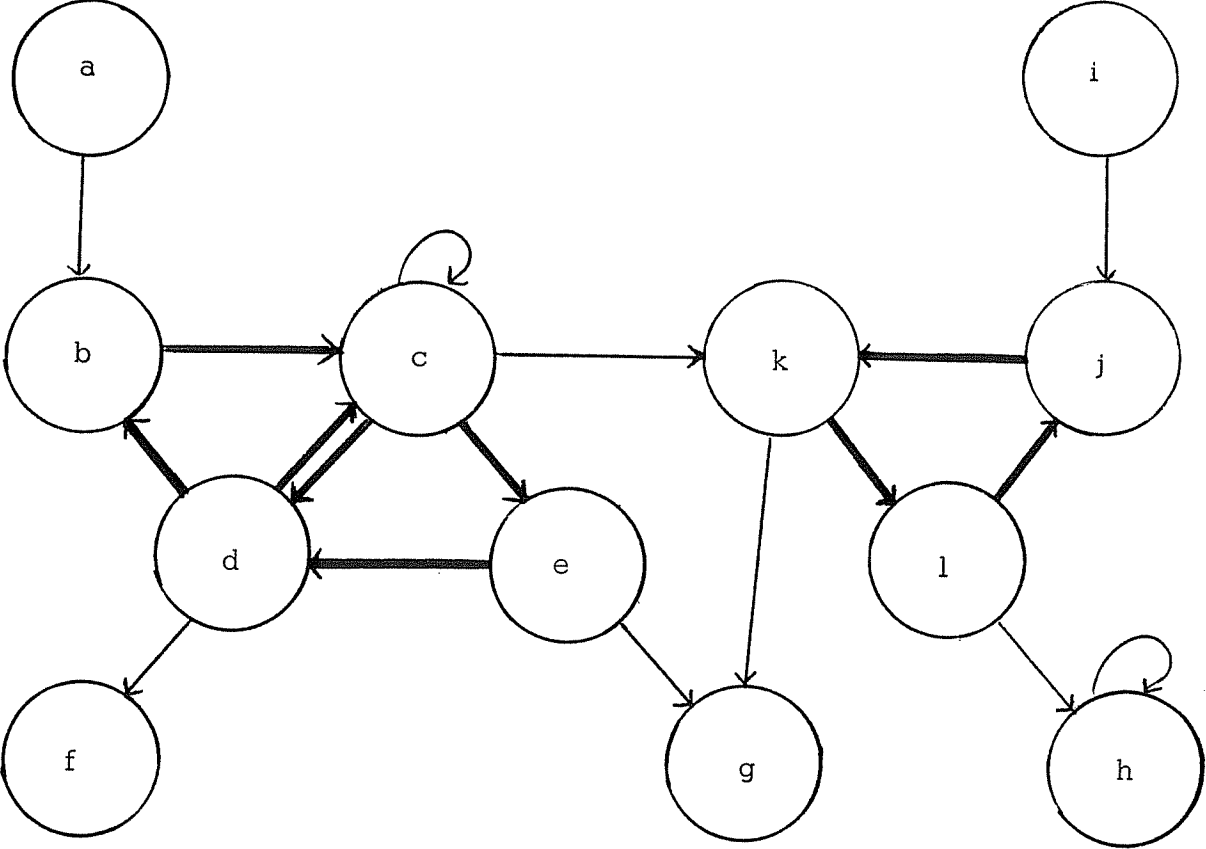
\includegraphics[width=.49\linewidth]{../img/purdom_g1.png}
    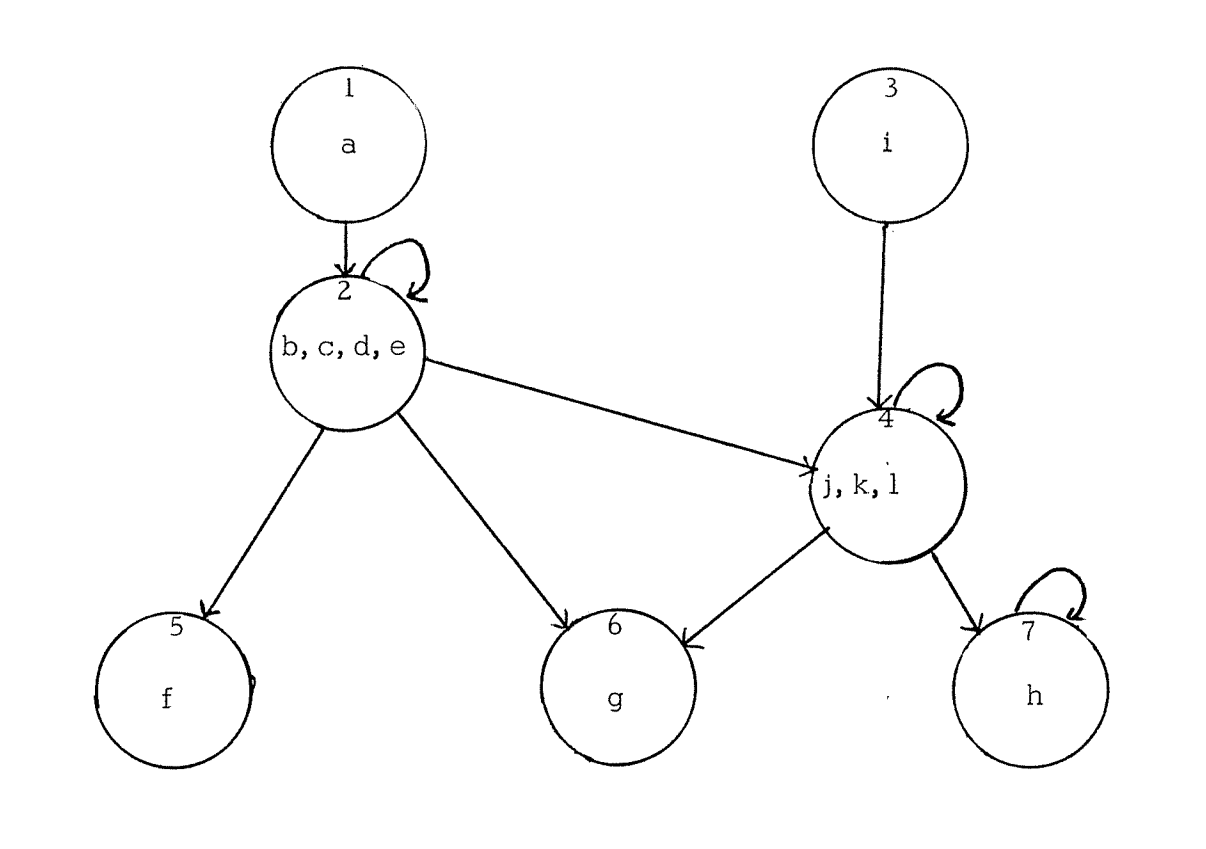
\includegraphics[width=.49\linewidth]{../img/purdom_g2b.png}
    \caption{aus \cite[Seite 78]{purdom1970transitive}}
\end{figure}

\begin{minipage}[t]{.5\textwidth}
test1
\end{minipage}
\begin{minipage}[t]{.5\textwidth}
test2
\end{minipage}

%\end{comment}

%% algo

\section{Vergleich der Suchalgorithmen}

Wie bereits erwähnt erfolgt die horizontale Suche pro Kode über alle Versionen ohne Vorkenntnisse vorheriger Suchergebnisse. Im Gegensatz dazu verarbeitet die vertikale Suche pro Version alle Kodes nur einmal, ist also allein deshalb schon effizienter, wenn Umsteiger für mehr als einen Kode ermittelt werden sollen. 

Wenn die Daten zusätlich aus einer Datenbank gelesen werden, ist die Anzahl an Aufrufen der readData-Funktion wesentlich entscheidender als die Menge an Ergebnissen pro Aufruf. Denn das Verbinden mit der Datenbank und Auslösen eines Suchbefehls dauert eine gewisse Zeit, was sich bei sehr vielen Aufrufen schnell aufaddiert. Dementsprechend ist es wesentlich schneller, alle Umsteiger einer Version auf einmal zu lesen, statt einzeln. 

Andererseits würde wiederum das Abfragen zusätzlicher Informationen, wie beispielsweise der Titel der Kodes eines Umsteigers vorher und nachher, bei der vertikalen Suche schnell die Größe der Daten im Arbeitsspeicher ansteigen lassen, weil pro Aufruf immer alle Umsteiger pro Version zwischengespeichert werden. 

Daher werden die beiden Algorithmen für unterschiedliche Zwecke eingesetzt.

Horizontale Suche:

\begin{itemize}
\item Darstellung der Umsteiger eines einzelnen Kodes mit Zusatzinformationen
\end{itemize}

Vertikale Suche: 

\begin{itemize}
\item Schreiben einer ConceptMap
\item Für alle Kodes einer Version bestimmen, ob diese Umsteiger haben (ja/nein)
\end{itemize}

\section{Schreiben der FHIR ConceptMap}
\label{write-conceptmap}

Dieser Abschnitt bezieht sich auf die in Kapitel \ref{conceptmap-structure} beschriebene ConceptMap-Struktur. 

Die anonyme Funktion, die der vertikalen Suche übergeben werden kann, dient zum Schreiben der ConceptMap. Jeder Aufruf der Funktion innerhalb des Algorithmus verfügt über die Daten, die zum Schreiben einer \emph{group} an Umsteigern mit Start- und Zielversion benötigt werden. Ein Durchlauf der vertikalen Suche kann dann mehrere Gruppen generieren, die ein Mapping auf eine Zielversionen ausgehend von allen anderen Versionen des Kodiersystems ermöglichen. Ebenfalls kann die Kombination mehrerer vertikalen Suche für jede Version als Zielversion aufgerufen werden, um so eine ConceptMap von allen Versionen auf alle Versionen zu schreiben.

Eine alle Versionen umfassende ConceptMap wird jedoch sehr groß. Zum Beispiel für die ICD-10-GM mit allen Kodes aus allen Versionen im XML-Format ist die Datei circa 1 GB groß. Wie in \cite{braaksma2014streaming} beschrieben macht es Sinn solche Dateien zu streamen, denn andernfalls müsste die komplette Datei im Arbeitsspeicher des Servers geschrieben werden. Die Vorgehensweise über die anonymen Funktionen ermöglicht genau das Streaming, weil nach jedem Aufruf der Ausgabepuffer des Servers geleert werden kann. Ein weiterer Vorteil ist, dass selbst wenn ein User sehr große ConceptMaps generieren lässt, der Download-Fortschritt über das Streaming angezeigt wird.  

Konkret enthält jede Iteration der anonymen Funktion die Informationen über Zielversion, aktuelle verarbeitete Version, sowie die vereinigten Umsteiger über alle vorher verarbeiteten Versionen. Zusätzlich muss allerdings noch bekannt sein, welche Kodes insgesamt in der Startversion vorhanden sind; zum einen, um Kodes ohne Umsteiger abzudecken und zum anderen, um keine Umsteiger aus vorher verarbeiteten Version aufzunehmen, deren Ursprungskode in der aktuellen Version nicht existiert. Hierfür ist also ein weiterer readData-Aufruf notwendig. Aus dem Vergleich dieser Kodes mit den Einträgen in der Merge-Datenstruktur können die Relationen für das Mapping bestimmt werden:

{
\renewcommand{\arraystretch}{1.2}
%\setlength{\tabcolsep}{12pt}
\begin{tabular}{ll}
%\uzlemph{Kode} & \uzlemph{Titel} \\
Kode in Merge-Daten enthalten? & Relation (R4) \\
\hline
Nein & \emph{equivalent} \\
Ja, übergeleitet auf UNDEF & \emph{unmatched} \\
Ja, übergeleitet auf einen Kode & \emph{related-to} \\
Ja, überleitetet auf mehrere Kodes & \emph{wider} \\
\end{tabular}
}

%, weil wie in (§Verweis) beschrieben die Liste der vereinigten Umsteiger immer auch Einträge aus vorher verarbeiteten Versionen enthalten durch die rückwärts topologische Vorgehensweise bedingt. Also zum Beispiel Kodes die in neueren Versionen erst hinzukommen. Außerdem wird über die beiden Informationen Umsteiger über die Versionen zwischen Start und Ziel sowie Kodes der Startversion die relationship bestimmt.

%Kode in Startversion;  Kode in Vereinigte Umsteiger; relationship
%vorhanden; Liste an Umsteigern; wider
%vorhanden; ein Umsteiger; related-to
%vorhanden; => UNDEF; unmapped
%vorhanden; nicht vorhanden; equivalent

Ablauf des Schreibens einer ConceptMap mit einer einzelnen Zielversion: 

\begin{enumerate}
\item Anfang der ConceptMap schreiben: \emph{ConceptMap}, \emph{url}, \emph{id}.
\item Vertikale Suche mit anonymer Funktion starten; jeder Aufruf generiert eine \emph{group}. \newline
Für jeden Kode wird ein \emph{element$\rightarrow$code}, \emph{element$\rightarrow$target$\rightarrow$code} Paar geschrieben -- \newline oder bei Relation \emph{wider} entsprechend mehrere \emph{target$\rightarrow$code} Einträge. 
\item Ende der ConceptMap schreiben.
\end{enumerate}

%Außerdem erlaubt die Vorgehensweise mit der anonymen Funktion ein Streaming der Datei. Das heißt muss nicht erst komplett im Arbeitsspeicher erstellt werden. Selbst wenn Umsteiger von allen Versionen als Start auf alle Versionen als Ziel geschrieben werden soll, werden als Daten im Arbeitsspeicher nur maximal die Sammlung der vereinigten Umsteiger von Start zu Ziel (oder andersherum) 

Eine Beispiel-ConceptMap im XML-Format befindet sich im Appendix \ref{conceptmap-example}.



\chapter{Web-Applikation} PHP Verwendung https://w3techs.com/technologies/details/pl-php

Version Control: thomas2019pragmatic (data1)

\section{Symfony}

\subsection{Controller}

Routing

\subsection{Serializer}

XML

CSV

SQL-Insert

\subsection{Console}

\subsection{Template-Engine Twig}

\subsection{Http Foundation}

Request

Response

StreamedResponse

\subsection{HttpClientInterface}

Download

\subsection{File System}

\subsection{UUID}

\section{Backend}

\subsection{Setup-XML}

\subsection{Konsole}

\subsection{Doctrine}

\subsection{Datenbank / MySQL}

\section{Frontend}

\subsection{Webpack / Node.js}

\subsection{Bootstrap}

Layout, Nav-Tabs, Modal, Icons

\subsection{SCSS}

\subsection{Tooltips}

\section{AJAX}

Modal

BfArM/Dimdi Links

\section{}

\newpage 

Model-View-Controller \citep[Seite 176f]{voorhees2020guide}

\begin{figure}[H]
    \centering
    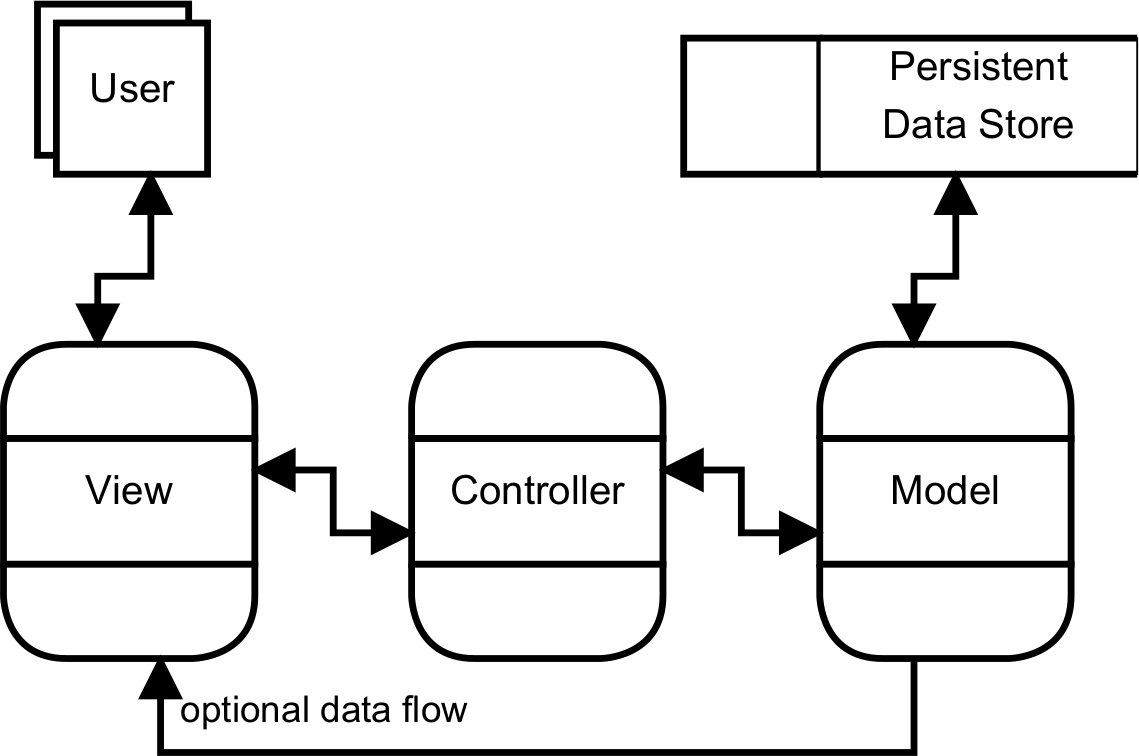
\includegraphics[width=.7\linewidth]{../img/mvc.png}
    \caption{\citep[Seite 177]{voorhees2020guide}}
\end{figure}

Abstraction and Decoupling

Symfony \citep{potencier2022symfony}

Dependency Injection \citep{seemann2019dependency}

When to stream? \citep{braaksma2014streaming}

CSS Flexbox \citep{flexbox-csstricks}

Programming Languages Harmful \citep{janssenscan}

\section{Anonyme Funktionen}

Callback

Zum Schreiben der ConceptMap

Data-Preprocessing

InsertEncoder

https://dev.mysql.com/doc/refman/en/insert-optimization.html


\chapter{Zusammenfassung} \section{Ergebnisse}

\subsection{Gegenseitige Validierung / Intra-DB Validierung}

\cite{intradbvalid}

\subsection{Patienten-DB}

\begin{figure}[H]
    \centering
    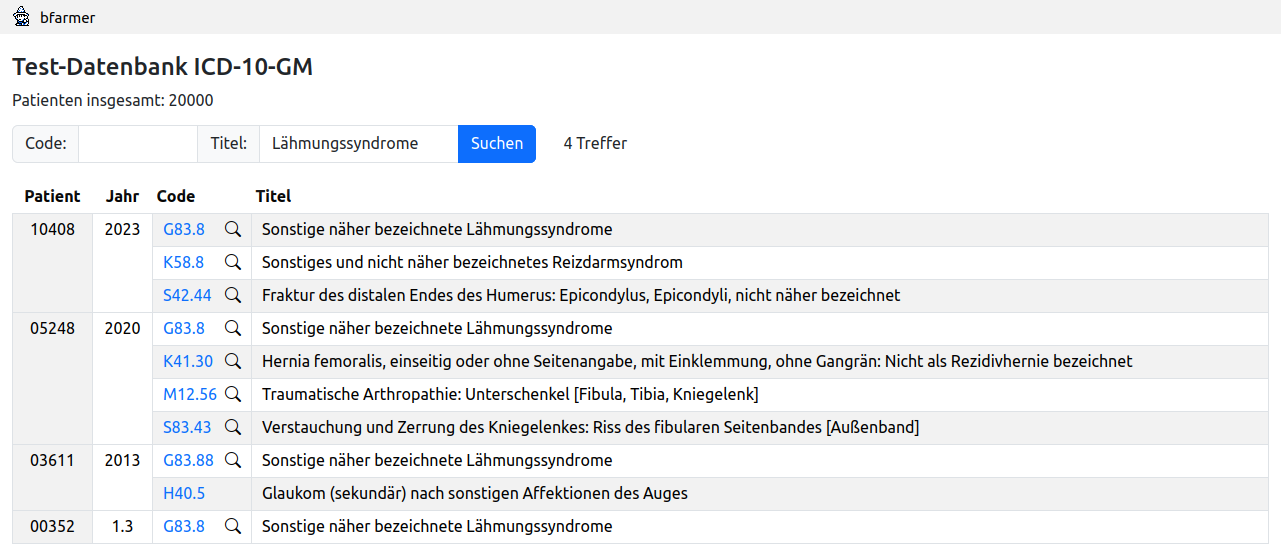
\includegraphics[width=.8\linewidth]{../img/patients_screenshot.png}
    \caption{Patienten}
\end{figure}

\begin{figure}[H]
    \centering
    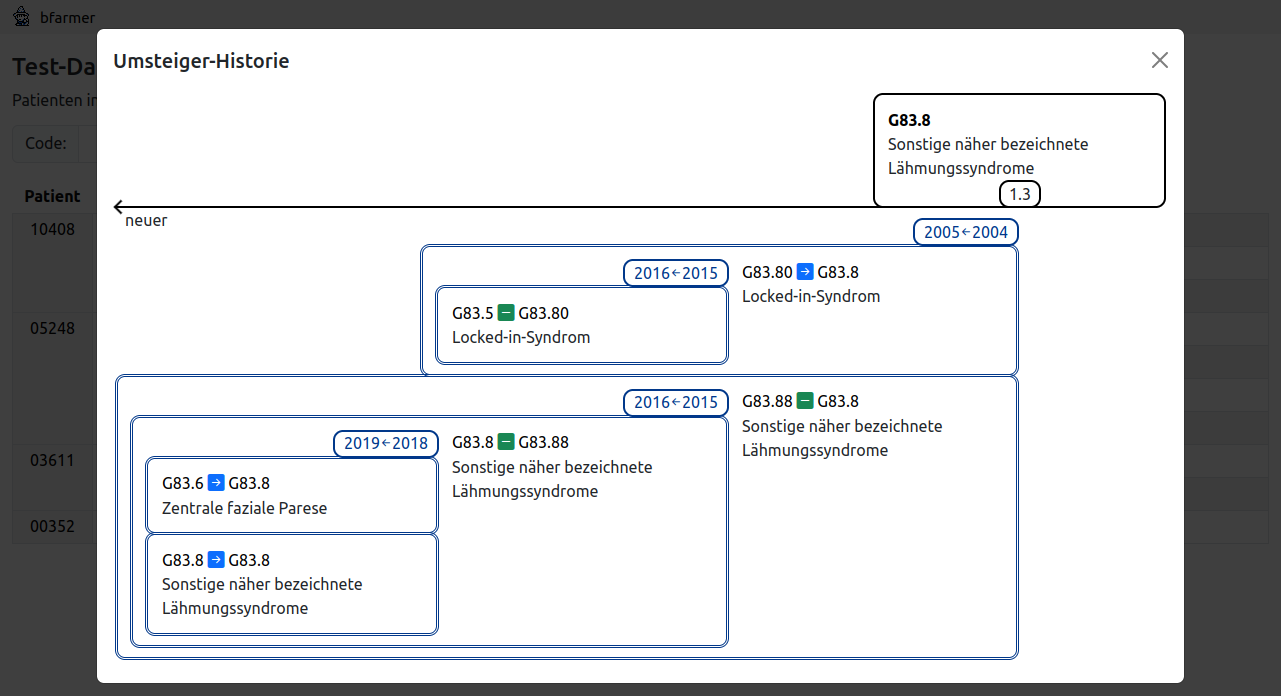
\includegraphics[width=.8\linewidth]{../img/umsteiger_screenshot.png}
    \caption{Umsteiger}
\end{figure}

Integration:

\begin{enumerate}
\item Bootstrap
\item CSS-Datei
\item On-Click Event
\item Ajax-Funktion
\end{enumerate}

\subsection{Mapping Quality}

\section{Zusammenfassung}

\section{Ausblick}

\subsection{RESTful (nach außen und innen / mehr AJAX)}

\subsection{ATC}

ATC \cite[ATC-Klassifikation]{bfarmatc}

PDF \cite{poppler}

\subsection{Sessions}

\subsection{Caching}



\newpage
\begin{Code}
curl -X 'POST' \
  'http://localhost:8080/fhir/ConceptMap' \
  -H 'accept: application/fhir+json' \
  -H 'Content-Type: application/fhir+xml' \
  -d "@/home/simon/Downloads/conceptmap_r4_icd10gm_2024.xml"
\end{Code}

\begin{Code}
curl -X 'GET' \
  'http://localhost:8080/fhir/ConceptMap/$translate?code=G83.8&system=1.3' \
  -H 'accept: application/fhir+json'
\end{Code}

\begin{comment}
\newpage

\begin{Code}
{
  "resourceType": "Parameters",
  "parameter": [ {
    "name": "result",
    "valueBoolean": true
  }, {
    "name": "message",
    "valueString": "Matches found"
  }, {
    "name": "match",
    "part": [ {
      "name": "equivalence",
      "valueCode": "wider"
    }, {
      "name": "concept",
      "valueCoding": {
        "system": "2024",
        "code": "G83.6"
      }
    }, {
      "name": "source",
      "valueUri": "urn:uuid:0192f4d0-20da-7a03-9f2e-a50d9266aeee"
    } ]
  }, {
    "name": "match",
    "part": [ {
      "name": "equivalence",
      "valueCode": "wider"
    }, {
      "name": "concept",
      "valueCoding": {
        "system": "2024",
        "code": "G83.8"
      }
    }, {
      "name": "source",
      "valueUri": "urn:uuid:0192f4d0-20da-7a03-9f2e-a50d9266aeee"
    } ]
  }, {
    "name": "match",
    "part": [ {
      "name": "equivalence",
      "valueCode": "wider"
    }, {
      "name": "concept",
      "valueCoding": {
        "system": "2024",
        "code": "G83.5"
      }
    }, {
      "name": "source",
      "valueUri": "urn:uuid:0192f4d0-20da-7a03-9f2e-a50d9266aeee"
    } ]
  } ]
\end{Code}
\end{comment}


\appendix
\chapter{Appendix}
\section{Abweichungen zwischen ICD-10-GM und OPS Versionen}
\label{abweichungen-versionen}

\subsection{ICD-10-GM}

\begingroup
\renewcommand{\arraystretch}{1.2}
\begin{longtable}{|c|l|l|}
\hline\hline

\umsteigerTabelleKopf\hline\hline

\umsteigerTabelleZeileUCUS{2025}
{version2025-vorab/icd10gm2025syst-ueberl-vorab.zip}
{Klassifikationsdateien/icd10gm2025syst\_vorab.txt}
{Klassifikationsdateien/\umsteigerTabelleCodeBreak
icd10gm2025syst\_umsteiger\_2024\_2025\_vorab.txt\umsteigerTabelleCodeBreakEnd}
{$\cdot$ Vorab-Version}
\hline\hline

\umsteigerTabelleZeileUU{2024}
{version2024/icd10gm2024syst-ueberl.zip}
{Klassifikationsdateien/\umsteigerTabelleCodeBreak icd10gm2024syst\_umsteiger\_2023\_20221206\_2024.txt\umsteigerTabelleCodeBreakEnd}
\hline\hline

\umsteigerTabelleZeileUCU{2023}
{version2023/icd10gm2023syst-ueberl\_20221206.zip}
{Klassifikationsdateien/\umsteigerTabelleCodeBreak icd10gm2023syst\_20221206.txt\umsteigerTabelleCodeBreakEnd}
{Klassifikationsdateien/\umsteigerTabelleCodeBreak icd10gm2023syst\_umsteiger\_2022\_2023\_20221206.txt\umsteigerTabelleCodeBreakEnd}
\hline\hline

\umsteigerTabelleZeileUS{2022}{vorgaenger/icd10gm2022.zip}{$\cdot$ Zip-Unterdatei: \texttt{icd10gm2022syst-ueberl.zip}}\hline\hline

\umsteigerTabelleZeileUV{2021}{vorgaenger/icd10gm2021.zip}{icd10gm2021syst-ueberl-20201111}\hline\hline
\umsteigerTabelleZeileUV{2020}{vorgaenger/icd10gm2020.zip}{icd10gm2020syst-ueberl}\hline\hline
\umsteigerTabelleZeileUV{2019}{vorgaenger/icd10gm2019.zip}{icd10gm2019syst-ueberl}\hline\hline

\umsteigerTabelleZeileUV{2018}{vorgaenger/icd10gm2018.zip}{x1gut2018}\hline\hline
\umsteigerTabelleZeileUV{2017}{vorgaenger/icd10gm2017.zip}{x1gut2017}\hline\hline
\umsteigerTabelleZeileUV{2016}{vorgaenger/icd10gm2016.zip}{x1gut2016}\hline\hline
\umsteigerTabelleZeileUV{2015}{vorgaenger/icd10gm2015.zip}{x1gut2015}\hline\hline

\umsteigerTabelleZeileUV{2014}{vorgaenger/icd10gm2014.zip}{x1gua2014}\hline\hline
\umsteigerTabelleZeileUV{2013}{vorgaenger/icd10gm2013.zip}{x1gua2013}\hline\hline

\umsteigerTabelleZeileUCU{2012}
{vorgaenger/icd10gm2012.zip}
{x1ueb2011\_2012/Klassifikationsdateien/\umsteigerTabelleCodeBreak icd10gmsyst2012.txt\umsteigerTabelleCodeBreakEnd}
{x1ueb2011\_2012/Klassifikationsdateien/\umsteigerTabelleCodeBreak umsteiger\_icd10gmsyst2011\_icd10gmsyst2012.txt\umsteigerTabelleCodeBreakEnd}
\hline\hline

\umsteigerTabelleZeileUCU{2011}
{vorgaenger/icd10gm2011.zip}
{x1ueb2010\_2011/Klassifikationsdateien/\umsteigerTabelleCodeBreak icd10gmsyst2011.txt\umsteigerTabelleCodeBreakEnd}
{x1ueb2010\_2011/Klassifikationsdateien/\umsteigerTabelleCodeBreak umsteiger\_icd10gmsyst2010\_icd10gmsyst2011.txt\umsteigerTabelleCodeBreakEnd}
\hline\hline

\umsteigerTabelleZeileUCU{2010}
{vorgaenger/icd10gm2010.zip}
{x1ueb2009\_2010/Klassifikationsdateien/\umsteigerTabelleCodeBreak icd10gmsyst2010.txt\umsteigerTabelleCodeBreakEnd}
{x1ueb2009\_2010/Klassifikationsdateien/\umsteigerTabelleCodeBreak umsteiger\_icd10gmsyst2009\_icd10gmsyst2010.txt\umsteigerTabelleCodeBreakEnd}
\hline\hline

\umsteigerTabelleZeileUCU{2009}
{vorgaenger/icd10gm2009.zip}
{x1ueb2008\_2009/Klassifikationsdateien/\umsteigerTabelleCodeBreak icd10gmsyst2009.txt\umsteigerTabelleCodeBreakEnd}
{x1ueb2008\_2009/Klassifikationsdateien/\umsteigerTabelleCodeBreak umsteiger\_icd10gmsyst2008\_icd10gmsyst2009.txt\umsteigerTabelleCodeBreakEnd}
\hline\hline

\umsteigerTabelleZeileUCUS{2008}
{vorgaenger/icd10gm2008.zip}
{x1ueb2007\_2008/Klassifikationsdateien/\umsteigerTabelleCodeBreak
icd10v2008.txt\umsteigerTabelleCodeBreakEnd}
{x1ueb2007\_2008/Klassifikationsdateien/\umsteigerTabelleCodeBreak
umsteiger20072008.txt\umsteigerTabelleCodeBreakEnd}
{$\cdot$ ISO-8859-1}
\hline\hline

\umsteigerTabelleZeileUCUS{2007}
{vorgaenger/icd10gm2007.zip}
{x1ueb2006\_2007/Klassifikationsdateien/\umsteigerTabelleCodeBreak
ICD10V2007.txt\umsteigerTabelleCodeBreakEnd}
{x1ueb2006\_2007/Klassifikationsdateien/\umsteigerTabelleCodeBreak
Umsteiger.txt\umsteigerTabelleCodeBreakEnd}
{$\cdot$ ISO-8859-1}
\hline\hline

\umsteigerTabelleZeileUCUS{2006}
{vorgaenger/icd10gm2006.zip}
{x1ueb2005\_2006/ICD10V2006.txt}
{x1ueb2005\_2006/umsteiger.txt}
{$\cdot$ ISO-8859-1}
\hline\hline

\umsteigerTabelleZeileUCUS{2005}
{vorgaenger/icd10gm2005.zip}
{x1ueb2004\_2005/ICD10V2005.txt}
{x1ueb2004\_2005/umsteiger.txt}
{$\cdot$ ISO-8859-1}
\hline\hline

\umsteigerTabelleZeileUCUS{2004}
{vorgaenger/icd10gm2004.zip}
{x1ueb20\_2004/icd10v2004.txt}
{x1ueb20\_2004/Umsteiger.txt}
{$\cdot$ ISO-8859-1\newline$\cdot$ Punkt-Strich-Notation\newline$\cdot$ 6-Spalten-Umsteiger}
\hline\hline

\umsteigerTabelleZeileUCUS{2.0}
{vorgaenger/icd10gm20.zip}
{x1ueb13\_20\_v11/icd10v20.txt}
{x1ueb13\_20\_v11/Umsteiger.txt}
{$\cdot$ ISO-8859-1\newline$\cdot$ Punkt-Strich-Notation\newline$\cdot$ Kreuz-Stern-System\newline$\cdot$ 6-Spalten-Umsteiger\newline$\cdot$ Nicht endständige Umsteiger}
\hline\hline

\umsteigerTabelleZeileLetzte{1.3}
{x1ueb13\_20\_v11/icd10v13.txt}
{$\cdot$ ISO-8859-1\newline$\cdot$ Punkt-Strich-Notation\newline$\cdot$ Kreuz-Stern-System\newline$\cdot$ Keine Überleitung}
\hline\hline

\end{longtable}
\endgroup

\newpage

\subsection{OPS}

\begingroup
\renewcommand{\arraystretch}{1.2}
\begin{longtable}{|c|l|l|}
\hline\hline

\umsteigerTabelleKopf\hline\hline

\umsteigerTabelleZeileUCUS{2025}
{version2025-vorab/ops2025syst-ueberl-vorab.zip}
{Klassifikationsdateien/ops2025syst\_vorab.txt}
{Klassifikationsdateien/\umsteigerTabelleCodeBreak
ops2025syst\_umsteiger\_2024\_2025\_vorab.txt\umsteigerTabelleCodeBreakEnd}
{$\cdot$ Vorab-Version}
\hline\hline

\umsteigerTabelleZeileU{2024}{version2024/ops2024syst-ueberl.zip}\hline\hline

\umsteigerTabelleZeileU{2023}{version2023/ops2023syst-ueberl.zip}\hline\hline

%\umsteigerTabelleAnmerkung{Für Version 2022 waren die Überleitungsdateien enthalten als eigene Zip-Datei zusammen mit allen anderen Dateien in einer großen Zip-Datei.}\hline\hline

\umsteigerTabelleZeileUS{2022}{vorgaenger/ops2022.zip}{$\cdot$ Zip-Unterdatei: \texttt{ops2022syst-ueberl.zip}}\hline\hline

%\umsteigerTabelleAnmerkung{Bis Version 2021 lagen die Überleitungsdateien in einem Unterverzeichnis zusammen in einer Zip-Datei, welche auch allen anderen Dateien für eine Version enthielt.}\hline\hline

\umsteigerTabelleZeileUV{2021}{vorgaenger/ops2021.zip}{ops2021syst-ueberl}\hline\hline
\umsteigerTabelleZeileUV{2020}{vorgaenger/ops2020.zip}{ops2020syst-ueberl}\hline\hline
\umsteigerTabelleZeileUV{2019}{vorgaenger/ops2019.zip}{ops2019syst-ueberl}\hline\hline
\umsteigerTabelleZeileUV{2018}{vorgaenger/ops2018.zip}{p1sut2018}\hline\hline
\umsteigerTabelleZeileUV{2017}{vorgaenger/ops2017.zip}{p1sut2017}\hline\hline
\umsteigerTabelleZeileUV{2016}{vorgaenger/ops2016.zip}{p1sut2016}\hline\hline
\umsteigerTabelleZeileUV{2015}{vorgaenger/ops2015.zip}{p1sut2015}\hline\hline

\umsteigerTabelleZeileUCU{2014}
{vorgaenger/ops2014.zip}
{p1sua2014-20131104/Klassifikationsdateien/\umsteigerTabelleCodeBreak ops2014syst\_20131104.txt\umsteigerTabelleCodeBreakEnd}
{p1sua2014-20131104/Klassifikationsdateien/\umsteigerTabelleCodeBreak ops2014syst\_umsteiger\_2013\_2014\_20131104.txt\umsteigerTabelleCodeBreakEnd}
\hline\hline

\umsteigerTabelleZeileUCU{2013}
{vorgaenger/ops2013.zip}
{p1sua2013/Klassifikationsdateien/\umsteigerTabelleCodeBreak ops2013syst\_20121113.txt\umsteigerTabelleCodeBreakEnd}
{p1sua2013/Klassifikationsdateien/\umsteigerTabelleCodeBreak ops2013syst\_umsteiger\_2012\_2013\_20121109.txt\umsteigerTabelleCodeBreakEnd}
\hline
\pagebreak
\hline

\umsteigerTabelleZeileUCU{2012}
{vorgaenger/ops2012.zip}
{p1ueb2011\_2012/Klassifikationsdateien/\umsteigerTabelleCodeBreak opssyst2012.txt\umsteigerTabelleCodeBreakEnd}
{p1ueb2011\_2012/Klassifikationsdateien/\umsteigerTabelleCodeBreak umsteiger\_opssyst2011\_opssyst2012.txt\umsteigerTabelleCodeBreakEnd}
\hline\hline

\umsteigerTabelleZeileUCU{2011}
{vorgaenger/ops2011.zip}
{p1ueb2010\_2011/Klassifikationsdateien/\umsteigerTabelleCodeBreak opssyst2011.txt\umsteigerTabelleCodeBreakEnd}
{p1ueb2010\_2011/Klassifikationsdateien/\umsteigerTabelleCodeBreak umsteiger\_opssyst2010\_opssyst2011.txt\umsteigerTabelleCodeBreakEnd}
\hline\hline

\umsteigerTabelleZeileUCU{2010}
{vorgaenger/ops2010.zip}
{p1ueb2009\_2010/Klassifikationsdateien/\umsteigerTabelleCodeBreak opssyst2010.txt\umsteigerTabelleCodeBreakEnd}
{p1ueb2009\_2010/Klassifikationsdateien/\umsteigerTabelleCodeBreak umsteiger\_opssyst2009\_opssyst2010.txt\umsteigerTabelleCodeBreakEnd}
\hline\hline

\umsteigerTabelleZeileUCUS{2009}
{vorgaenger/ops2009.zip}
{p1ueb2008\_2009/Klassifikationsdateien/\umsteigerTabelleCodeBreak opsamtl2009.txt\umsteigerTabelleCodeBreakEnd}
{p1ueb2008\_2009/Klassifikationsdateien/\umsteigerTabelleCodeBreak umsteigeramtl20082009.txt\umsteigerTabelleCodeBreakEnd}
{$\cdot$ ISO-8859-1\newline$\cdot$ None statt UNDEF\newline$\cdot$ 6-Spalten-Umsteiger (altes Format)}
\hline\hline

\umsteigerTabelleZeileUCUS{2008}
{vorgaenger/ops2008.zip}
{ops2008amtl/p1ueb2007\_2008/\umsteigerTabelleCodeBreak
Klassifikationsdateien/opsamtl2008.txt\umsteigerTabelleCodeBreakEnd}
{ops2008amtl/p1ueb2007\_2008/\umsteigerTabelleCodeBreak
Klassifikationsdateien/umsteigeramtl20072008.txt\umsteigerTabelleCodeBreakEnd}
{$\cdot$ ISO-8859-1\newline$\cdot$  None statt UNDEF\newline$\cdot$ 6-Spalten-Umsteiger (altes Format)}
\hline\hline

\umsteigerTabelleZeileUCUS{2007}
{vorgaenger/ops2007.zip}
{ops2007amtl/p1ueb2006\_2007/\umsteigerTabelleCodeBreak
Klassifikationsdateien/opsamtl2007.txt\umsteigerTabelleCodeBreakEnd}
{ops2007amtl/p1ueb2006\_2007/\umsteigerTabelleCodeBreak
Klassifikationsdateien/UmsteigerAmtlich.txt\umsteigerTabelleCodeBreakEnd}
{$\cdot$ ISO-8859-1\newline$\cdot$ None statt UNDEF\newline$\cdot$ 6-Spalten-Umsteiger (altes Format)}
\hline
\pagebreak
\hline

\umsteigerTabelleZeileUCUS{2006}
{vorgaenger/ops2006.zip}
{ops2006amtl/p1ueb2005\_2006/opsv2006.txt}
{ops2006amtl/p1ueb2005\_2006/umsteiger.txt}
{$\cdot$ ISO-8859-1\newline$\cdot$ None statt UNDEF\newline$\cdot$ 6-Spalten-Umsteiger (altes Format)}
\hline\hline

\umsteigerTabelleZeileUCUS{2005}
{vorgaenger/ops2005.zip}
{ops2005amtl/p1ueb2004\_2005\_v10/OPS2005.txt}
{ops2005amtl/p1ueb2004\_2005\_v10/umsteiger.txt}
{$\cdot$ ISO-8859-1\newline$\cdot$ None statt UNDEF\newline$\cdot$ 5-Spalten-Umsteiger}
\hline\hline

\umsteigerTabelleZeileUCUS{2004}
{vorgaenger/ops2004.zip}
{ops2004amtl/p1ueb21\_2004\_v10/opsv2004.txt}
{ops2004amtl/p1ueb21\_2004\_v10/Umsteiger.txt}
{$\cdot$ ISO-8859-1\newline$\cdot$ 4-Spalten-Umsteiger}
\hline\hline

\umsteigerTabelleZeileUCUS{2.1}
{vorgaenger/ops21.zip}
{ops21amtl/p1ueb20\_21\_v10/opsv21.txt}
{ops21amtl/p1ueb20\_21\_v10/Umsteiger.txt}
{$\cdot$ ISO-8859-1\newline$\cdot$ KOMBI-Kode\newline$\cdot$ 6-Spalten-Umsteiger (ursprüngliches Format)}
\hline\hline

\umsteigerTabelleZeileUCUS{2.0}
{vorgaenger/ops20.zip}
{p1ueb11\_20\_v11/Opsv20.txt}
{p1ueb11\_20\_v11/Umsteiger.txt}
{$\cdot$ ISO-8859-1\newline$\cdot$ KOMBI-Kode\newline$\cdot$ 3-Spalten-Umsteiger}
\hline\hline

\umsteigerTabelleZeileLetzte{1.1}
{p1ueb11\_20\_v11/Opsv11.txt}
{$\cdot$ ISO-8859-1\newline$\cdot$ Keine Überleitung}
\hline\hline

%\umsteigerTabelleAnmerkung{Für Version 1.1 werden nur die Kodes aus Version 2.0 genommen.}\hline\hline

\end{longtable}
\endgroup

%\newpage
%\section{Beispielergebnis der Horizontalen Suche}
\label{search-horizontal-example}

Ergebnis für den Aufruf \texttt{searchHorizontal('icd10gm', '2014', 'M21.6')} im JSON-Format. Um Platz zu sparen enthält nur der erste Umsteiger die zusätzlichen Informationen, die pro Eintrag ermittelt werden, also die automatische Überleitbarkeit sowie die Titel der Kodes. Außerdem sind für die Lesbarkeit die Sonderzeichen nicht kodiert. 

\begin{minipage}[t]{.5\linewidth}\vspace{0pt}
\begin{tcolorbox}[center,width=\linewidth,colback=white,colframe=white]
\footnotesize
\begin{verbatim}
{
  "fwd": {
    "year": "2014",
    "other": "2015",
    "umsteiger": [
      {
        "old": "M21.6",
        "new": "M21.60",
        "auto": "",
        "auto_r": "A",
        "old_name": "Sonstige erworbene
Deformitäten des Knöchels und des Fußes",
        "new_name": "Erworbener Hohlfuß
[Pes cavus]"
      },
      {
        "old": "M21.6",
        "new": "M21.61",
      },
      {
        "old": "M21.6",
        "new": "M21.62",
      },
      {
        "old": "M21.6",
        "new": "M21.63",
      },
      {
        "old": "M21.6",
        "new": "M21.68",
      }
    ]
  },
\end{verbatim}
\end{tcolorbox}
\end{minipage}
\begin{minipage}[t]{.5\linewidth}\vspace{0pt}
\begin{tcolorbox}[center,width=\linewidth,colback=white,colframe=white]
\footnotesize
\begin{verbatim}
  "rev": {
    "year": "2013",
    "other": "2012",
    "umsteiger": [
      {
        "old": "M21.60",
        "new": "M21.6",
        "recursion": {
          "year": "2.0",
          "other": "1.3",
          "umsteiger": [
            {
              "old": "M21.6",
              "new": "M21.60",
            }
          ]
        }
      },
      {
        "old": "M21.67",
        "new": "M21.6",
        "recursion": {
          "year": "2.0",
          "other": "1.3",
          "umsteiger": [
            {
              "old": "M21.6",
              "new": "M21.67",
            }
          ]
        }
      },
      {
        "old": "M21.87",
        "new": "M21.6",
        "recursion": {
          "year": "2.0",
          "other": "1.3",
          "umsteiger": [
            {
              "old": "M21.8",
              "new": "M21.87",
            }
          ]
        }
      }
    ]
  }
}
\end{verbatim}
\end{tcolorbox}
\end{minipage}

\newpage
\section{Beispielergebnis der Horizontalen Suche}
\label{search-horizontal-example}

Ergebnis im JSON-Format für den Aufruf: \newline \texttt{searchHorizontal('icd10gm', '2014', 'M21.6')}

Um Platz zu sparen enthält nur der erste Umsteiger die zusätzlichen Informationen, die pro Eintrag ermittelt werden, also die automatische Überleitbarkeit sowie die Titel der Kodes. Außerdem sind für die Lesbarkeit die Sonderzeichen nicht kodiert.

Die Seite zeigt die Richtung 2024$\leftarrow$2014 und die nächste Seite 2014$\rightarrow$2004, 2.0, 1.3. \\

\begin{Code}
{
  "fwd": {
    "year": "2014",
    "other": "2015",
    "umsteiger": [
      {
        "old": "M21.6",
        "new": "M21.60",
        "auto": "",
        "auto_r": "A",
        "old_name": "Sonstige erworbene Deformitäten des Knöchels und des Fußes",
        "new_name": "Erworbener Hohlfuß [Pes cavus]"
      },
      {
        "old": "M21.6",
        "new": "M21.61",
      },
      {
        "old": "M21.6",
        "new": "M21.62",
      },
      {
        "old": "M21.6",
        "new": "M21.63",
      },
      {
        "old": "M21.6",
        "new": "M21.68",
      }
    ]
  },







  "rev": {
    "year": "2013",
    "other": "2012",
    "umsteiger": [
      {
        "old": "M21.60",
        "new": "M21.6",
        "recursion": {
          "year": "2.0",
          "other": "1.3",
          "umsteiger": [
            {
              "old": "M21.6",
              "new": "M21.60",
            }
          ]
        }
      },
      {
        "old": "M21.67",
        "new": "M21.6",
        "recursion": {
          "year": "2.0",
          "other": "1.3",
          "umsteiger": [
            {
              "old": "M21.6",
              "new": "M21.67",
            }
          ]
        }
      },
      {
        "old": "M21.87",
        "new": "M21.6",
        "recursion": {
          "year": "2.0",
          "other": "1.3",
          "umsteiger": [
            {
              "old": "M21.8",
              "new": "M21.87",
            }
          ]
        }
      }
    ]
  }
}
\end{Code}


\newpage
\section{Beispiel ConceptMap}
\label{conceptmap-example}

FHIR ConceptMap im XML-Format für das Beispiel in Abbildung \ref{vertical-example}. Die komplette ConceptMap enthält noch viel mehr Gruppen und Kodes, aber abgedruckt sind nur die relevanten Teile wie beschrieben in Unterabschnitt \ref{vert-search} -- "`Konkretes Beispiel"'. \\

\begin{Code}
<?xml version="1.0"?>
<ConceptMap xmlns="http://hl7.org/fhir">
  <id value="icd10gm_from:2024_to:1.3_target:2024"/>
  <url value="urn:uuid:0192e098-0871-79d5-a4e6-039398aa7803"/>

<group>
  <source value="2018"/>
  <target value="2024"/>
  <element>
    <code value="G83.8"/>
    <target>
      <code value="G83.6"/>
      <equivalence value="wider"/>
    </target>
    <target>
      <code value="G83.8"/>
      <equivalence value="wider"/>
    </target>
  </element>
</group>

<group>
  <source value="2015"/>
  <target value="2024"/>
  <element>
    <code value="G83.80"/>
    <target>
      <code value="G83.5"/>
      <equivalence value="relatedto"/>
    </target>
  </element>
  <element>
    <code value="G83.88"/>
    <target>
      <code value="G83.6"/>
      <equivalence value="wider"/>
    </target>
    <target>
      <code value="G83.8"/>
      <equivalence value="wider"/>
    </target>
  </element>
</group>

<group>
  <source value="2004"/>
  <target value="2024"/>
  <element>
    <code value="G83.8"/>
    <target>
      <code value="G83.6"/>
      <equivalence value="wider"/>
    </target>
    <target>
      <code value="G83.8"/>
      <equivalence value="wider"/>
    </target>
    <target>
      <code value="G83.5"/>
      <equivalence value="wider"/>
    </target>
  </element>
</group>

<group>
  <source value="1.3"/>
  <target value="2024"/>
  <element>
    <code value="G83.8"/>
    <target>
      <code value="G83.6"/>
      <equivalence value="wider"/>
    </target>
    <target>
      <code value="G83.8"/>
      <equivalence value="wider"/>
    </target>
    <target>
      <code value="G83.5"/>
      <equivalence value="wider"/>
    </target>
  </element>
</group>
</ConceptMap>
\end{Code}


\end{document}
